\documentclass[11pt]{report} % Define la clase de documento como 'report' con tamaño de fuente 11pt
\usepackage{geometry} % Paquete para personalizar los márgenes del documento
\usepackage[utf8]{inputenc} % Permite la introducción de caracteres UTF-8
\usepackage[greek, spanish, es-tabla]{babel} % Establece idiomas para el documento
\usepackage[bottom]{footmisc} % Coloca las notas al pie en la parte inferior de la página
\usepackage[tt]{titlepic} % Permite incluir una imagen en la página de título con una fuente mono-spaced
\usepackage{url} % Permite la inserción de URL en el documento
\usepackage{xurl} % Mejora el manejo de URL en el documento
\usepackage{graphicx} % Permite la inclusión de gráficos en el documento
\usepackage{makeidx} % Facilita la creación de índices
\usepackage{enumerate} % Permite la personalización de listas enumeradas
\usepackage{lastpage} % Proporciona una referencia a la última página del documento
\usepackage{fancyhdr, ragged2e} % Personaliza los encabezados y pies de página
\usepackage{eurosym} % Permite la inserción del símbolo de euro
\usepackage{float} % Mejora el posicionamiento de los elementos flotantes en el documento
\usepackage{titlesec} % Facilita la personalización de títulos de secciones
\usepackage{hyperref} % Permite la creación de enlaces hipertexto
\usepackage{nameref} % Permite hacer referencia al nombre de secciones
\usepackage{enumitem} % Permite personalizar listas
\usepackage{booktabs} % Mejora la apariencia de las tablas
\usepackage[table]{xcolor} % Permite el uso de colores en tablas
\usepackage{multirow} % Permite combinar celdas en tablas
\usepackage{amsmath} % Proporciona funciones matemáticas avanzadas
\usepackage{tikz} % Permite la creación de gráficos vectoriales
\usetikzlibrary{shadings} % Carga la librería para degradados en los gráficos de TikZ
\usepackage[nameinlink]{cleveref} % Facilita las referencias cruzadas con nombres
\usepackage{listings} % Permite la inclusión de código fuente en el documento
\usepackage{microtype} % Para mejor formato de texto
\usepackage[normalem]{ulem} % Para subrayado con color
\usepackage{palatino} %La fuente Libertine también se ve bien
\usepackage[T1]{fontenc}


% Ajustes de los márgenes de la página
\addtolength{\oddsidemargin}{-.8in}
\addtolength{\evensidemargin}{-.8in}
\addtolength{\textwidth}{1.45in}
\addtolength{\topmargin}{-.1in}
\addtolength{\textheight}{1.25in}


\graphicspath{{figures/}} % Directorio donde se encuentran los archivos de imágenes
\pagestyle{fancy} % Estilo de página personalizado
\renewcommand{\chaptermark}[1]{\markboth{\scriptsize\MakeUppercase{#1}}{}} % Configuración del marcado de capítulos
\renewcommand{\sectionmark}[1]{\markright{\tiny\MakeUppercase{#1}}{}} % Configuración del marcado de secciones


% Configuración del pie de página
\fancypagestyle{plain}{
    \renewcommand{\headrulewidth}{0pt} 
    \fancyfoot[L]{\raisebox{-0.6cm}{
\includegraphics[height=1cm]{figures/EscudoUniovi.jpg}}}
    \fancyfoot[C]{\scriptsize BidMon Universe. Plataforma de coleccionismo de cartas digitales. \\ Trabajo Fin de Grado Ingeniería Informática del Software \textbar{} Versión 0.1 \\ Paula Suárez Prieto}
    \fancyfoot[R]{\thepage\ de \pageref{LastPage}}
    \renewcommand{\footrulewidth}{0.4pt}
}




%Evita warnings de cabecera
\setlength{\headheight}{15pt}
\setcounter{secnumdepth}{4}

%Esto es para poder ponerle un formato bien hecho a los \paragraph{}
\titleformat{\paragraph}
{\normalfont\normalsize\bfseries}{\theparagraph}{1em}{}
\titlespacing*{\paragraph}
{0pt}{3.25ex plus 1ex minus .2ex}{1.5ex plus .2ex}

%Y esto para para ponerselo a los \subparagraph{}
\titleformat{\subparagraph}
{\normalfont\normalsize\bfseries}{\theparagraph}{1em}{}
\titlespacing*{\subparagraph}
{0pt}{1ex plus 1ex minus .2ex}{1.5ex plus .2ex}

% Configuración para permitir la numeración hasta el quinto nivel
\setcounter{secnumdepth}{5}

% Crear un nuevo contador para subsubsubsection que se reinicia con cada subsubsection
\newcounter{subsubsubsection}[subsubsection]

% Formatear el contador para que se muestre como subsubsection.subsubsubsection
\renewcommand{\thesubsubsubsection}{\thesubsubsection.\arabic{subsubsubsection}}

\newcommand{\subsubsubsection}[1]{%
  \refstepcounter{subsubsubsection}
  \paragraph{#1}\vspace{3mm}
}


% Formato para el título de subsubsubsection
\titleformat{\paragraph}
  {\normalfont\normalsize\bfseries\itshape}{\thesubsubsubsection}{1em}{}
\titlespacing*{\paragraph}
  {0pt}{3.25ex plus 1ex minus .2ex}{-1ex plus .2ex}


% Colores usados en las tablas
\definecolor{headercolor}{rgb}{.871,  .918,  .965}
\definecolor{rowcolor}{rgb}{.949,  .949,  .949}
\definecolor{darkgreen}{rgb}{0.525, 0.655, 0.537}
\definecolor{lightgreen}{rgb}{0.824, 0.890, 0.784}
\definecolor{linkColor}{HTML}{086554}


% Configuración de los estilos del capítulo
\titleformat{\chapter}[display]
  {\normalfont\huge\bfseries\raggedright}
  {\color{darkgreen}\chaptertitlename\ \thechapter}{20pt}{\Huge\color{black}\raggedright}

% Estilos de los enlaces 
\hypersetup{
    colorlinks = true, % Colores en los enlaces 
    linkcolor = linkColor, % Color de los enlaces internos
    filecolor = linkColor, % Color de los enlaces a archivos
    urlcolor = linkColor, % Color de los enlaces externos
    citecolor = linkColor
}

% Comando para subrayar enlaces
\newcommand{\coloredUnderline}[1]{\bgroup\markoverwith{\textcolor{linkColor}{\rule[-0.5ex]{2pt}{0.4pt}}}\ULon{#1}}


\phantomsection
\makeindex

\begin{document}
\selectlanguage{spanish} 


\hypersetup{pageanchor=false}

% ----- Portada -----
\begin{titlepage}
	\centering
	
\includegraphics[width=0.2\textwidth]{EscudoUniovi}
	\hspace{3 cm}
	
\includegraphics[width=0.3\textwidth]{EscudoEscuela}
	\par\vspace{1cm}
	
	\vspace{1.5cm}
	{\huge\bfseries BidMon Universe \\ Plataforma de coleccionismo de cartas digitales\par}
	\vspace{2cm}
	{\large \textbf{GRADO EN INGENIERÍA INFORMÁTICA DEL SOFTWARE} \par}
	\vspace{1cm}
	{\scshape\Large Trabajo Fin de Grado\par}
   	
  \vspace{2cm}
	\textbf{AUTOR}\par
	Paula Suárez Prieto \\
	\vspace{1.5cm}
	\textbf{TUTOR}\par
	Hugo Lebredo Buján
	\vfill
	
	{\large Julio 2024 \par}
\end{titlepage}
% ----- Fin Portada -----

% ----- Página de copyright -----
\newpage
\pagestyle{plain}
Copyright (C) 2020 \textbf{ELENA ALLEGUE GONZÁLEZ, JOSÉ MANUEL REDONDO LÓPEZ} \\
Teaching Innovation Project: PINN-19-A-029 (University of Oviedo)\\
This work has been published in \cite{RedondoPlantillasRG19} \cite{RedondoUCO20}\\
\\
Esta versión de la plantilla para Trabajos de Fin de Grado ha sido posible gracias a la donación de la ex-alumna Elena Allegue González de su documentación de Trabajo de Fin de Grado, que ha servido como base para elaborar esta versión. Aquí podréis encontrar todos los títulos y subtítulos de las secciones, pero las explicaciones se mantendrán en la versión \textit{Word} de la plantilla (se proporciona una versión PDF de la misma para facilitar el acceso a las mismas). No obstante, del trabajo de Elena se han conservado ejemplos de como hacer elementos clave como imágenes, tablas, etc.

Desarrollar una versión \textit{Latex} de la plantilla desde cero es una trabajo bastante largo, pero gracias al trabajo de Elena se ha podido equiparar esta versión con las de \textit{Word} mucho más rápidamente.
% ----- Fin Página de copyright -----

%\newpage
\pagestyle{fancy}
\chapter*{Agradecimientos}

\pagestyle{fancy}

% Redefine el comando \chaptermark para personalizar el encabezado de los capítulos
\renewcommand{\chaptermark}[1]{ 
    % Marca ambos encabezados izquierdo y derecho con el título del capítulo
    \markboth{\scriptsize\MakeUppercase{#1}}{} 
}

% Redefine el comando \sectionmark para personalizar el encabezado de las secciones
\renewcommand{\sectionmark}[1]{ 
    % Marca el encabezado derecho con el título de la sección
    \markright{\tiny\MakeUppercase{#1}}{} 
}


%\Configuración del pie de página

\fancyfoot{}
\fancyfoot[L]{\raisebox{-0.6cm}{
\includegraphics[height=1cm]{figures/EscudoUniovi.jpg}}}

\fancyfoot[R] {\thepage\ de \pageref{LastPage}}
\fancyfoot[C]{\scriptsize BidMon Universe. Plataforma de coleccionismo de cartas digitales. \\ Trabajo Fin de Grado Ingeniería Informática del Software \textbar{} Versión 0.1 \\ Paula Suárez Prieto   }
\setlength{\footskip}{32.93277pt}
\renewcommand{\footrulewidth}{0.4pt}
\pagenumbering{arabic}


\pagestyle{plain}


\setcounter{tocdepth}{2}
\setcounter{secnumdepth}{4}

% ----- Página de Lista de contenidos -----
\pagestyle{plain}
{
  \hypersetup{hidelinks}
  \renewcommand{\thispagestyle}[1]{}
  \tableofcontents
}
\clearpage

% ----- Página de Lista de figuras -----
\newpage
{
  \hypersetup{hidelinks}
  \renewcommand{\thispagestyle}[1]{}
  \listoffigures
}
\clearpage

% ----- Página de Lista de tablas -----
\newpage
{
  \hypersetup{hidelinks}
  \renewcommand{\thispagestyle}[1]{}
  \listoftables
}
\clearpage

\newpage
\hypersetup{pageanchor=true}

\newpage


\newpage
\thispagestyle{empty}
\chapter{Introducción}
\noindent\begin{tikzpicture}
% Definir el degradado
\shade[left color=darkgreen, right color=lightgreen] (0,0) rectangle (\textwidth-1pt,0.2);

\end{tikzpicture}
\section{RESUMEN}
Las plataformas digitales han popularizado un modo de juego basado en la colección de cartas, permitiendo a los usuarios acceder a un mercado de intercambio de estas. 
Este modelo de juego genera miles de millones de euros al año, convirtiéndose en una de las formas de entretenimiento más destacadas en la actualidad.

Este trabajo presenta el desarrollo de una plataforma online de coleccionismo e intercambio de activos digitales, concretamente de cartas de Pokémon.
Esta plataforma permitirá a los usuarios adquirir sobres de cartas con distinta rareza, lo que añade un componente de exclusividad y emoción a la colección. 
Además, las cartas podrán ser subastadas en tiempo real, permitiendo a los usuarios adquirir las cartas más deseadas mediante pujas, mejorando así la experiencia de coleccionismo digital.

\section{PALABRAS CLAVE}
Coleccionismo, subastas, cartas, Pokémon

\section{\textit{ABSTRACT}}
Digital platforms have popularized a game mode based on card collecting, allowing users to access a marketplace for exchanging these cards. 
This gaming model generates billions of euros annually, becoming one of the most prominent forms of entertainment today.

This project presents the development of an online platform for the collection and exchange of digital assets, 
specifically Pokemon cards.
This platform will allow users to acquire packs of cards with varying rarities, 
adding a component of exclusivity and excitement to the collection. Additionally, the cards can be auctioned in real-time, 
allowing users to acquire the most desired cards through bids, thus enhancing the digital collecting experience.

\section{\textit{KEYWORDS}}
Collecting, auctions, cards, Pokemon


\newpage
\pagestyle{fancy}

%\newpage
\chapter{PLANIFICACIÓN DEL SISTEMA DE INFORMACIÓN}

\noindent\begin{tikzpicture}
% Definir el degradado
\shade[left color=darkgreen, right color=lightgreen] (0,0) rectangle (\textwidth-1pt,0.2);

\end{tikzpicture}
\newpage

\section{INICIO DEL PLAN DE SISTEMAS DE INFORMACIÓN}
\subsection{Análisis de la Necesidad del Plan de Sistemas de Información}
Con la tecnología, la forma en la que nos relacionamos con nuestros pasatiempos ha cambiado. La popularidad de plataformas como EA Sports FC y su modo Ultimate Team\cite{artsEASPORTSFC2023}, deja en evidencia que el mercado de coleccionismo digital está en pleno crecimiento \cite{sanmartin000MillonesDolares2021}. Sin embargo, aún existe un nicho de mercado específico por explorar: una plataforma dedicada exclusivamente al coleccionismo de cartas digitales.

BidMon Universe trata de dar respuesta a esta necesidad, ofreciendo a los coleccionistas digitales una forma segura e innovadora de comprar y vender activos digitales mediante un sistema de pujas ciego.

El Plan de Sistemas de Información para este proyecto se aborda desde una perspectiva que considera tanto la arquitectura técnica como la experiencia del usuario final. De esta manera se establece un marco de trabajo que garantiza que, además de cumplir con las expectativas del mercado actual, el proyecto proporciona características y experiencias novedosas que enriquecen la dinámica del coleccionismo digital.

\subsection{Identificación del Alcance del Plan de Sistemas de Información} \hypertarget{sec:2_identificacion_alcance_PSI}{}
La aplicación web a desarrollar deberá de proporcionar al usuario final las siguientes funcionalidades de alto nivel:
\begin{itemize}
    \item Todo usuario final puede acceder a la aplicación web y consultar la información sobre esta.
    \item Cualquier usuario, mayor de 18 años, tiene la posibilidad de crear una cuenta de usuario dentro de la aplicación.
    \item Cualquier usuario con una cuenta asociada en la aplicación puede iniciar sesión en esta.
    \item Los usuarios autenticados pueden recargar el saldo de su cuenta para posteriormente realizar compras en la aplicación.
    \item Los usuarios autenticados tendrán acceso a un catálogo de sobres de cartas que podrán adquirir si cuentan con saldo suficiente.
    \item Los usuarios autenticados podrán visualizar la colección de cartas adquiridas.
    \item Los usuarios autenticados tendrán la posibilidad de poner a la venta sus cartas.
    \item Los usuarios autenticados tendrán la posibilidad de comprar una carta directamente a otro jugador a través de subastas ciegas.
    \item Un usuario podrá retirar una puja antes de que el periodo de la subasta finalice.
    \item Los usuarios autenticados podrán consultar el mercado de subastas en cualquier momento.
    \item Los usuarios autenticados podrán consultar el histórico de transacciones realizadas.
    \item Los usuarios autenticados podrán consultar el estado de las subastas en las que ha participado, así como las que ha iniciado. 
    \item Los usuarios autenticados recibirán notificaciones informativas sobre las pujas realizadas y las subastas iniciadas.
    \item Los usuarios autenticados podrán modificar su perfil.
    \item Los usuarios autenticados podrán consultar el perfil de las personas que están subastando cartas. Se mostrará la siguiente información:
    \begin{itemize}
        \item Cartas destacadas del usuario. Por ejemplo, si este posee una carta rara podrá seleccionarla como destacada para mostrarla en su perfil.
        \item Número de pujas en las que ha participado.
        \item Número de subastas que ha realizado.
        \item Subastas activas.
        \item Tendrán la opción de añadir este usuario como favorito. ``Seguir'' al usuario para estar al día de sus subastas.
    \end{itemize}
    \item Un usuario con rol de administrador podrá acceder al histórico de subastas y cancelar las que considere fraudulentas, el sistema notificará al usuario que la ha iniciado.
\end{itemize}

En base a estas funcionalidades se extraen los siguientes \textbf{objetivos estratégicos} a lograr para alcanzar el éxito del proyecto:

\begin{itemize}
    \item Implementar un sistema de autenticación de usuarios.
    \item Implementar un sistema de venta de cartas.
    \item Implementar un sistema de subastas ciegas que permita a los usuarios comprar y vender cartas.
    \item Implememntar un sistema de gestión de subastas por parte de un usuario autenticado.
    \item Implememntar un sistema de gestión de subastas por parte de un usuario administrador.
    \item Implementar un sistema de notificaciones que informe a los usuarios sobre el estado de las subastas en las que participan.
    \item Interfaz intuitiva que permita al usuario realizar consultas sobre el estado de las pujas y subastas, además de visualizar la colección de cartas adquirida.
\end{itemize}

\subsection{Determinación de Responsables}
A continuación, se detallan las personas que participan en el proyecto junto con sus funciones.
\begin{itemize}
    \item El tutor del trabajo se encargará de la supervisión del proyecto.
    \item El alumno se encargará del desarrollo del proyecto y documentación de este. 
\end{itemize}

\newpage
\section{DEFINICIÓN Y ORGANIZACIÓN DEL PLAN DE SISTEMAS DE INFORMACIÓN}
 

\subsection{Especificación del Ámbito y Alcance} 


\subsection{Organización del Plan de Sistemas de Información }



\newpage
\section{ESTUDIO DE LA INFORMACIÓN RELEVANTE}
 
\subsection{Selección y Análisis de Antecedentes} 




%\newpage
\chapter{DEFINICIÓN DE LA ARQUITECTURA TECNOLÓGICA}
\noindent\begin{tikzpicture}
% Definir el degradado
\shade[left color=darkgreen, right color=lightgreen] (0,0) rectangle (\textwidth-1pt,0.2);

\end{tikzpicture}
\newpage
\section{Identificación de las Necesidades de Infraestructura Tecnológica} 

\newpage
\section{Selección de la Arquitectura Tecnológica} 

\newpage
\chapter{ESTUDIO DE VIABILIDAD DEL SISTEMA}
\noindent\begin{tikzpicture}
% Definir el degradado
\shade[left color=darkgreen, right color=lightgreen] (0,0) rectangle (\textwidth-1pt,0.2);

\end{tikzpicture}
\newpage


\section{ESTUDIO Y VALORACIÓN DE ALTERNATIVAS DE SOLUCIÓN. SELECCIÓN DE ALTERNATIVA FINAL}

\section{Análisis de sistemas similares}

En este apartado, se aborda un análisis detallado de las plataformas y sistemas que actualmente exhiben un comportamiento similar al del sistema que se pretende desarrollar para 'BidMon Universe'. 

La realización de este análisis es muy importante, ya que proporciona una base sólida para la toma de decisiones estratégicas. Al examinar detenidamente tanto las ventajas como las desventajas de los sistemas existentes, se identifican estrategias exitosas y se reconocen posibles fallos 
o áreas susceptibles de mejora. Este enfoque no solo informa las decisiones de diseño y tecnología, sino que también las fundamenta en un conocimiento práctico y bien contextualizado. Así, se garantiza que el desarrollo de 'BidMon Universe' esté 
armonizado con las tendencias actuales y adopte las soluciones más efectivas y adecuadas para su propósito.

El objetivo del proyecto es permitir a los usuarios coleccionar cartas e intercambiarlas mediante subastas, específicamente cartas de Pokémon. Por esta razón, se ha llevado a cabo un análisis de sistemas similares enfocados en los siguientes puntos:
\begin{itemize}
    \item Sistemas de intercambio de cartas digitales: Se analizarán diversos sistemas de intercambio de cartas digitales, destacando su relevancia en el mercado y las funcionalidades que ofrecen.
    \item Sistemas de subastas en línea: Se evaluarán plataformas de subastas en línea, analizando sus ventajas y desventajas, con el objetivo de identificar las mejores prácticas aplicables a nuestro proyecto.
    \item El mercado de coleccionistas de Pokémon: Se estudiará la extensa base de seguidores y coleccionistas de cartas Pokémon, comprendiendo su comportamiento, preferencias y el impacto que tienen en el mercado de subastas.
\end{itemize}

\subsection{Análisis de sistemas de intercambio de cartas digitales}
En esta sección se analizarán los sistemas de intercambio de cartas digitales, como EA Sports FC, NBA 2K y LaLiga Fantasy, que permiten a los usuarios adquirir y vender cartas de jugadores. 
Aunque el sistema de coleccionismo de cartas puede variar según la plataforma del juego, todos comparten una serie de características comunes. Estas incluyen la posibilidad de pujar 
por un jugador o comprarlo directamente, la existencia de distintas rarezas de cartas y la inclusión de eventos especiales.

\subsubsection{EA Sports FC}
\coloredUnderline{\href{https://www.ea.com/es-es/games/ea-sports-fc}{EA Sports FC}} es una destacada franquicia de videojuegos de fútbol disponible en diversas plataformas. 
Este análisis se centrará en el modo de juego \coloredUnderline{\href{https://www.ea.com/es-es/games/fifa/fifa-23/ultimate-team/item-guide}{FIFA Ultimate Team}}, 
que busca transformar la interacción de los jugadores, permitiéndoles construir y gestionar su propio equipo de fútbol. Los usuarios pueden buscar jugadores en el mercado de transferibles, 
pujar por ellos o comprarlos directamente. Además, pueden incrementar el valor de sus jugadores completando desafíos y cambiar la apariencia de las cartas. 
Este modo incluye tarjetas de jugadores con distintas rarezas, haciendo que algunas sean más valiosas que otras.

Se estima que EA Sports FC ha generado más de 6.000 millones de dólares en ingresos netos entre 2020 y 2025\cite{sanmartin000MillonesDolares2021}. En 2020, 
los ingresos casi se triplicaron en comparación con 2015, demostrando un crecimiento exponencial. El informe anual de Electronic Arts para el año fiscal 2023\cite{ea2023} 
especifica que se generaron 7.426 millones de dólares en ingresos netos y revela que el modo Ultimate Team de FIFA 23 es el más popular de la franquicia, con más de 10 millones 
de jugadores activos mensuales, siendo una de las mayores fuentes de ingresos de la empresa. El informe también destaca la intención de continuar desarrollando este mercado 
mediante la incorporación de nuevas características para el modo Ultimate Team.

La popularidad de este modo de juego ha llevado a Electronic Arts a lanzar una aplicación móvil llamada \coloredUnderline{\href{https://apps.apple.com/es/app/ea-sports-fc-24-companion/id1127108818}{EA SPORTS FC™ 24 Companion}}, 
que permite a los usuarios gestionar su club de FIFA Ultimate Team desde dispositivos móviles. Los usuarios necesitan tener el juego FIFA 24 para utilizar la aplicación, 
la cual se conecta a la cuenta del usuario en el juego. 

Desde la aplicación, los usuarios pueden comprar sobres de cartas, gestionar su plantilla, comprar jugadores en el mercado de transferibles y pujar por jugadores en subastas para utilizarlos posteriormente en el juego. 
Esta aplicación permite a los usuarios estar al tanto de las últimas novedades y ofertas del mercado, así como recibir notificaciones en tiempo real sobre el estado de sus pujas.

En las siguientes figuras, se muestra la interfaz de usuario de EA SPORTS FC™ 24 Companion.

\begin{figure}[H]
    \centering
    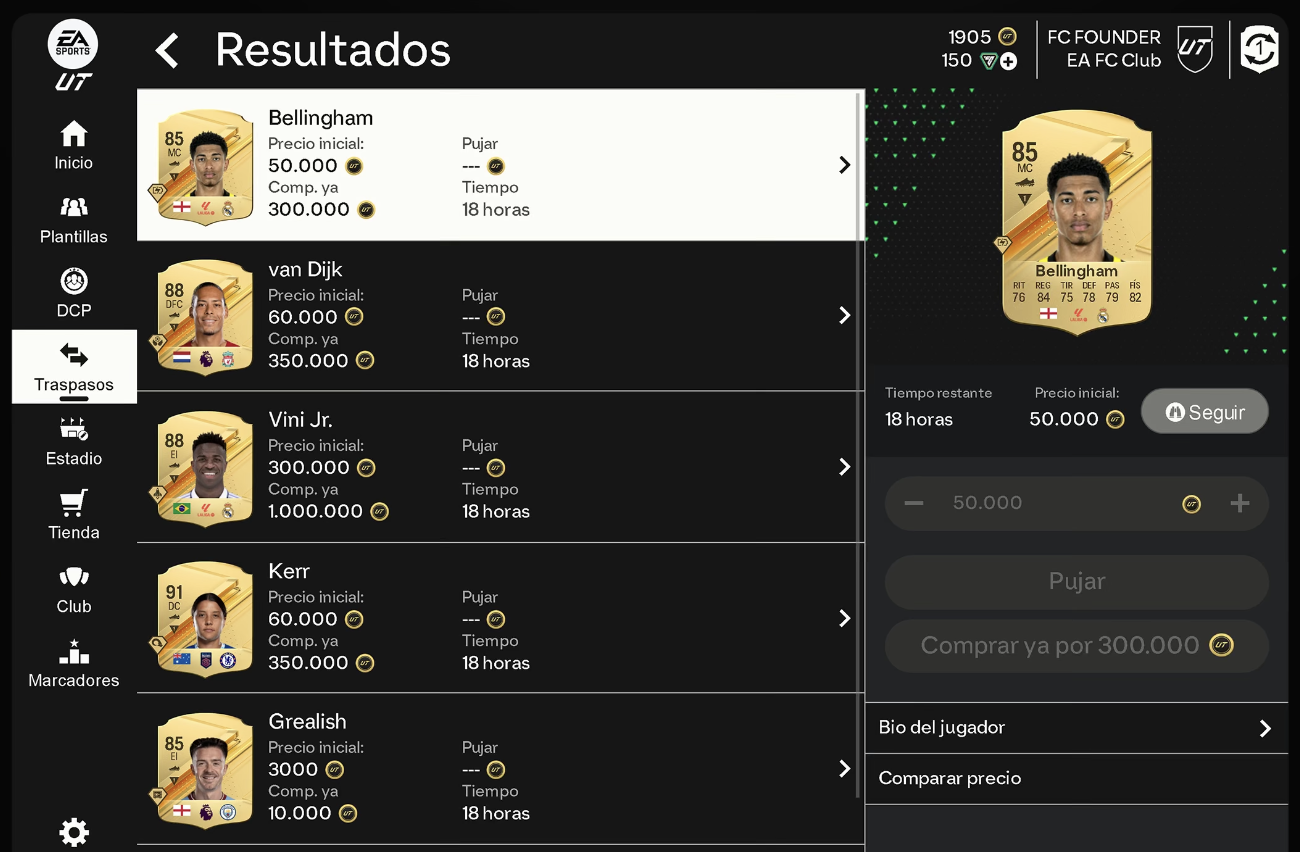
\includegraphics[width=0.7\textwidth]{figures/4-Estudio-viabilidad/4_FC_Companion.png}
    \caption{Página de traspasos de jugadores de EA SPORTS FC™ 24 Companion}
    \label{fig:ea_sports_fc_1}
    \hypertarget{fig:ea_sports_fc_1}{}
\end{figure}

\begin{figure}[H]
    \centering
    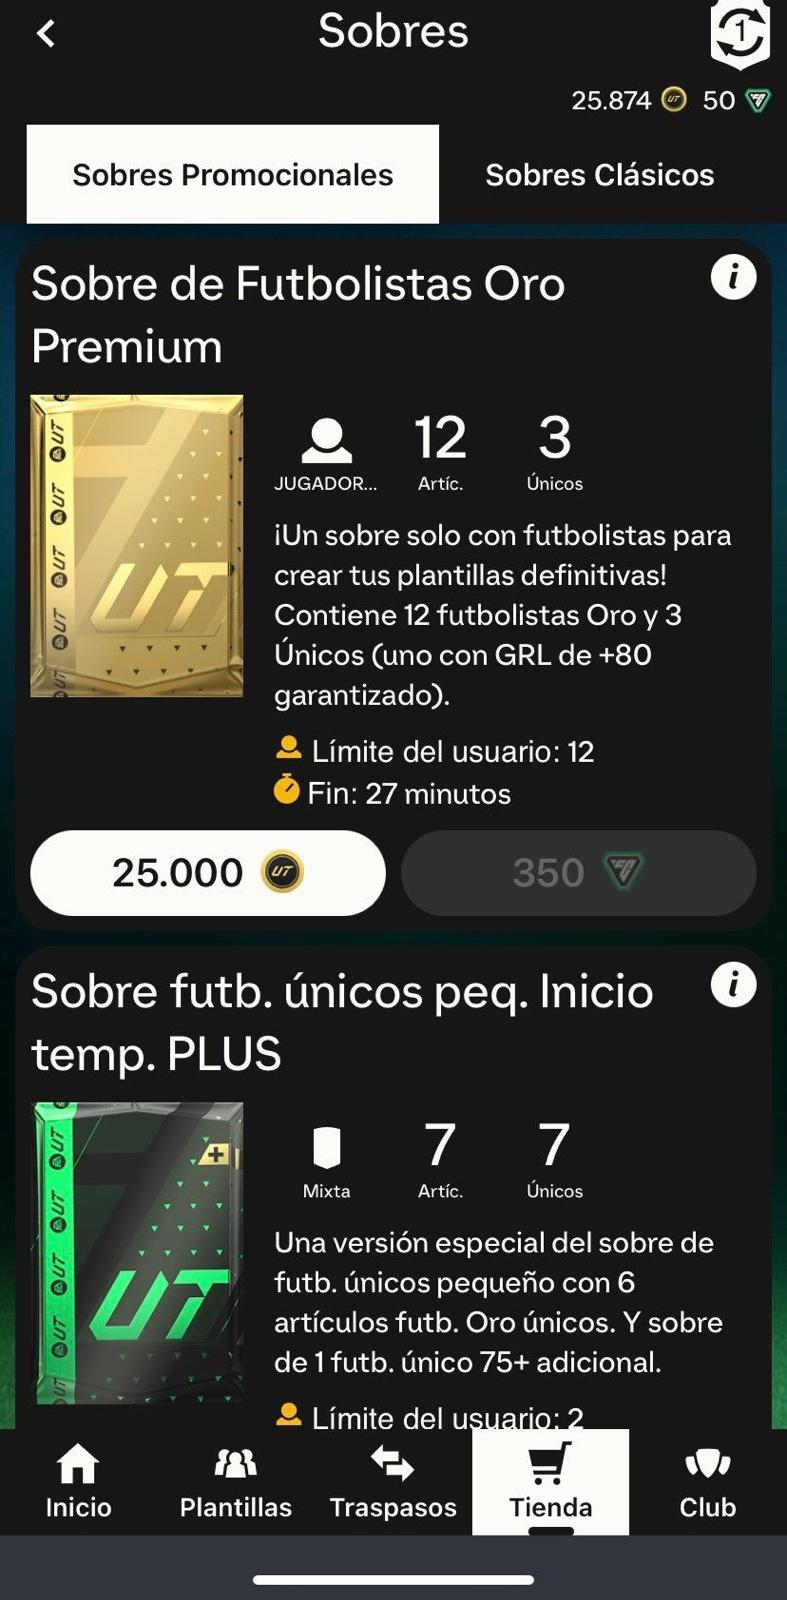
\includegraphics[width=0.3\textwidth]{figures/4-Estudio-viabilidad/4_FC_Companion2.jpeg}
    \caption{Página de compra de sobres de EA SPORTS FC™ 24 Companion}
    \label{fig:ea_sports_fc_2}
    \hypertarget{fig:ea_sports_fc_2}{}
\end{figure}

\subsubsubsection{Ventajas de EA Sports FC}
En el contexto de EA Sports FC, destacan las siguientes ventajas:
\begin{itemize}
    \item Los usuarios pueden marcar una carta para efectuar un seguimiento y recibir notificaciones en caso de una disminución en su precio.
    \item Se proporcionan estadísticas detalladas de cada carta, incluyendo su evolución de precio en las últimas semanas, así como los valores más bajos y más altos a los que se está vendiendo actualmente.
    \item Existe la opción de vender una carta directamente, evitando la necesidad de utilizar el sistema de subastas. 
    \item Cuenta con un buscador de ofertas que incorpora varios filtros.
    \item Los usuarios tienen la posibilidad de editar o cancelar sus pujas en curso.
    \item El sistema de subastas implementado opera bajo un mecanismo de puja ciega.
\end{itemize}

\subsubsubsection{Desventajas de EA Sports FC}
Sin embargo, es importante mencionar algunas desventajas de EA Sports FC, que incluyen:
\begin{itemize}
    \item Un número limitado de órdenes de canje simultáneas como, por ejemplo, el máximo de 25 permitido en EA Sports FC Mobile.
    \item Las pujas solo se pueden realizar por un valor igual o superior al establecido por el juego. 
\end{itemize}

\subsubsubsection{Ventajas del nuevo sistema respecto EA Sports FC}
El sistema en desarrollo presenta varias características que mejoran la experiencia del usuario en comparación con EA Sports FC.

\begin{itemize}
    \item El acceso a la aplicación es completamente gratuito.
    \item Ofrece una mayor personalización en el proceso de puja, brindando a los usuarios una experiencia más flexible y adaptada a sus preferencias.
    \item El usuario tiene la posibilidad de acceder a un histórico exhaustivo en el que se detallan todas las transacciones realizadas.
\end{itemize}

\subsubsection{NBA 2K}
\coloredUnderline{\href{https://nba.2k.com/}{NBA 2K}} es una destacada franquicia de videojuegos de baloncesto disponible en diversas plataformas. 
Este análisis se centrará en el modo de juego \coloredUnderline{\href{https://nba.2k.com/2k24/es-ES/myteam/}{MyTEAM}}, 
que busca transformar la interacción de los jugadores, permitiéndoles construir y gestionar su propio equipo de baloncesto. Los usuarios pueden buscar jugadores en el mercado de transferibles, 
pujar por ellos o comprarlos directamente. Existen distintos niveles de cartas para añadir un elemento de emoción al juego.
Existen también cartas de recompensa que se pueden obtener completando desafíos y eventos especiales.

Se estima que NBA 2K ha generado ingresos significativos en los últimos años. En el año fiscal 2023, 
los ingresos de Take-Two Interactive alcanzaron niveles récord gracias a sus franquicias principales, incluyendo NBA 2K. El informe anual de Take-Two Interactive para el año fiscal 2023\cite{take_two_2023} 
destaca que NBA 2K es una de las mayores fuentes de ingresos de la empresa, con una base de usuarios activa y comprometida, especialmente en el modo MyTEAM. 
En el informe se menciona la intención de seguir desarrollando este mercado ya que se espera que continúe creciendo en los próximos años.

La popularidad de este modo de juego ha llevado a Take-Two Interactive a lanzar una aplicación móvil llamada \coloredUnderline{\href{https://nba.2k.com/2k24/mynba-2k24/}{MyNBA 2K Companion App}}, 
que permite a los usuarios gestionar su equipo de MyTEAM desde dispositivos móviles. Los usuarios necesitan tener una cuenta de NBA 2K para utilizar la aplicación, 
la cual se conecta a la cuenta del usuario en el juego. 

La aplicaicón permite a los usuarios comprar sobres de cartas, gestionar su plantilla, comprar jugadores en el mercado de transferibles y pujar por jugadores en subastas para utilizarlos posteriormente en el juego.
Tiene otras funciones interesantes como la posibilidad de personalizar su propio jugador por medio de la función de escaneo facial, la cual permite a los usuarios escanear su rostro y añadirlo al juego.

En las siguientes figuras, se muestra la interfaz de usuario de NBA 2K Mobile.


\subsubsection{LaLiga Fantasy}
\coloredUnderline{\href{https://laligafantasy.relevo.com/}{LaLiga Fantasy}} un juego basado en la liga de fútbol española, conocida como LaLiga. En este juego, los usuarios tienen la capacidad de crear equipos que se componen de jugadores cuyo rendimiento se correlaciona con el desempeño real en los partidos de LaLiga. Además, existe la posibilidad de competir por premios reales en determinadas instancias del juego.
El juego dispone de un mercado en el que los usuarios pueden vender o adquirir jugadores a través de un sistema de subastas, por lo que estamos ante un escenario similar al anterior.

A continuación, se muestra la interfaz de usuario de LaLiga Fantasy.
\begin{figure}[H]
    \centering
    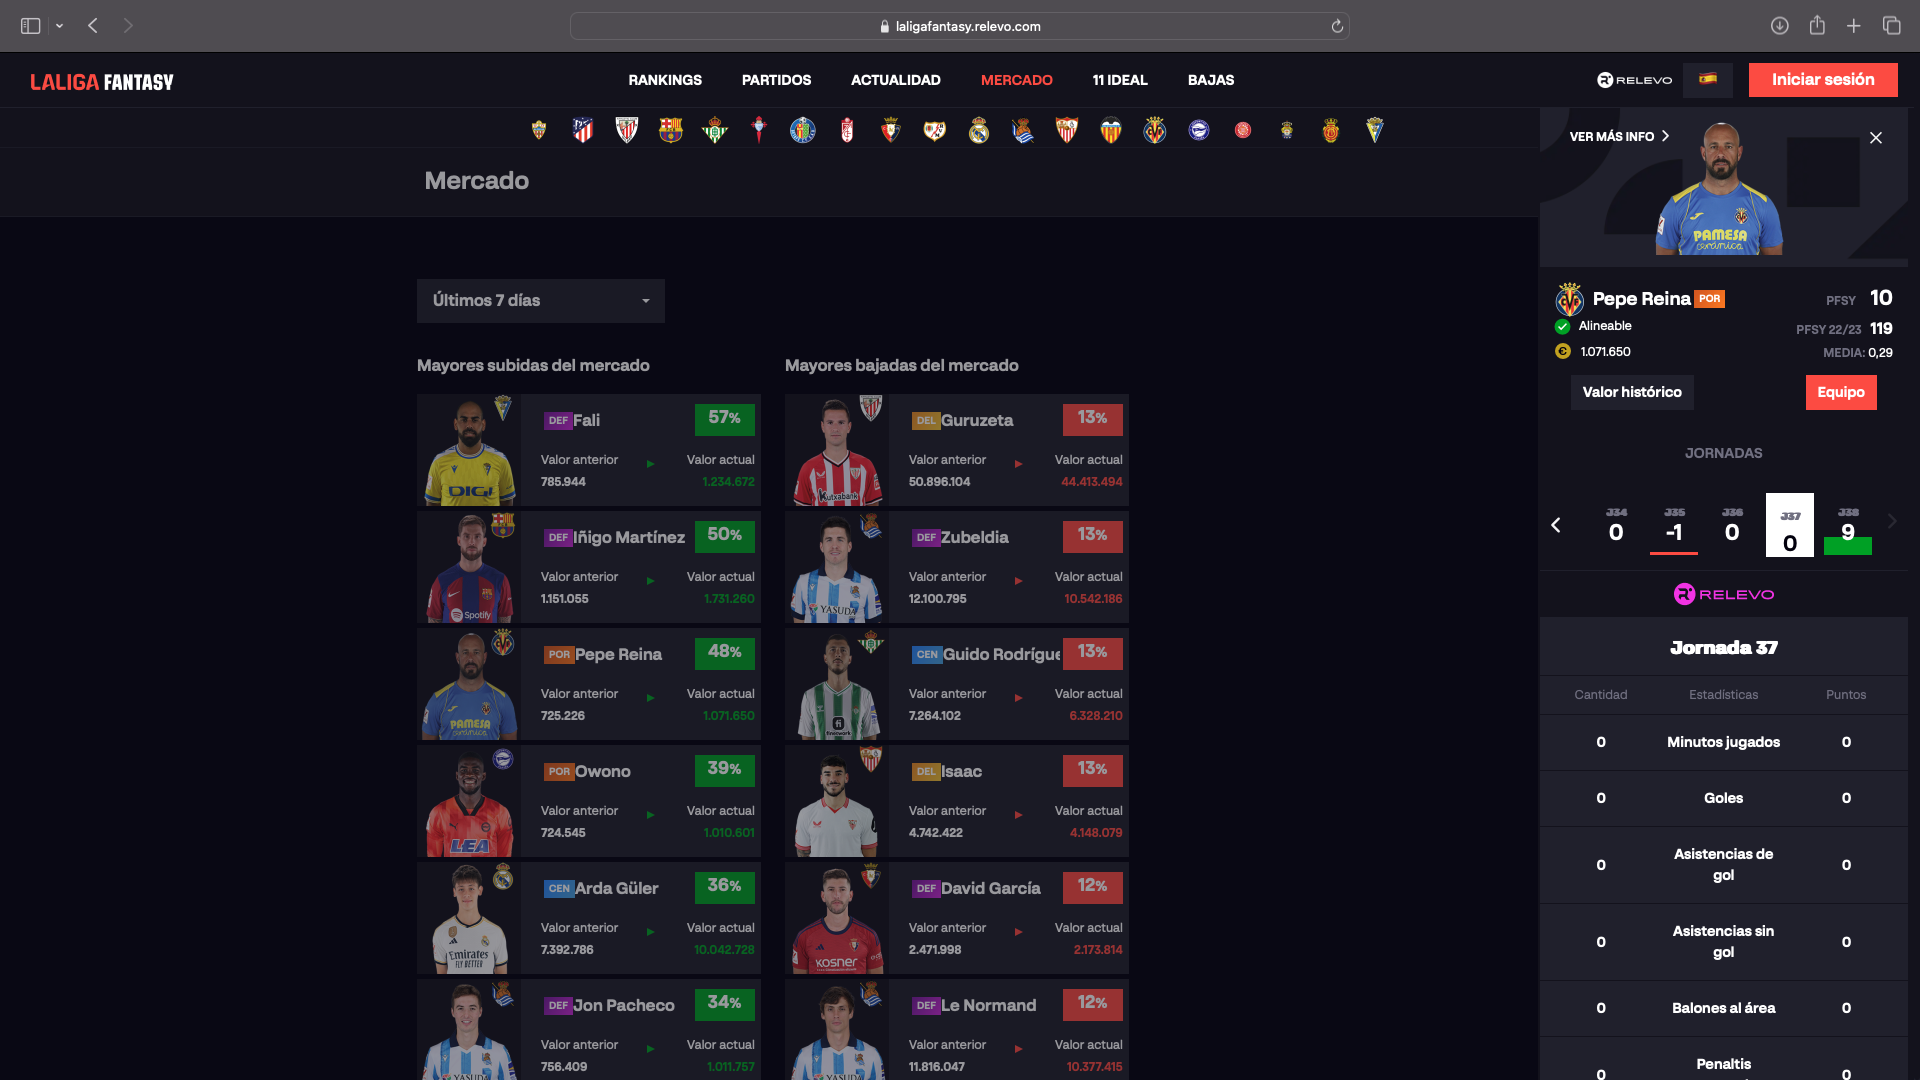
\includegraphics[width=0.7\textwidth]{figures/4-Estudio-viabilidad/4_LaLigaFantasy.png}
    \caption{Página de mercado de jugadores de LaLiga Fantasy}
    \label{fig:la_liga_fantasy}
    \hypertarget{fig:la_liga_fantasy}{}
\end{figure}

\subsubsubsection{Ventajas de LaLiga Fantasy}
Dentro del marco de LaLiga Fantasy, se destacan las siguientes características:
\begin{itemize}
    \item El juego renueva constantemente el mercado de transferibles.
    \item El juego cuenta con la capacidad de generar ofertas automáticas por los futbolistas que se encuentran en venta. Estas ofertas se establecen a partir de un valor aleatorio que oscila entre el valor de mercado del jugador, con un margen del 10\% tanto por encima como por debajo de dicho valor.
    \item Recientemente se ha incorporado el mercado de ``clausulazos'', donde los usuarios pueden adquirir un jugador pagando su cláusula, que será más elevada que el valor de mercado, sin tener que depender del propietario del jugador.
    \item Se pueden realizar ofertas por jugadores a otros usuarios.
\end{itemize}

\subsubsubsection{Desventajas de LaLiga Fantasy}
Se pueden identificar las siguientes desventajas:
\begin{itemize}
    \item La limitación a un máximo de 24 jugadores en la plantilla, lo que puede ocasionar la pérdida de oportunidades en subastas.
    \item La plataforma brinda escasa flexibilidad en lo que respecta a la personalización al momento de poner un jugador en venta.
\end{itemize}

\subsubsubsection{Ventajas del nuevo sistema respecto LaLiga Fantasy}
\begin{itemize}
    \item LaLiga Fantasy ofrece una suscripción de 0,99€/mes para poder jugar sin anuncios mientras que el sistema que se desarrollará carece de anuncios.
    \item Se proporciona un historial de transacciones completo para que los usuarios puedan rastrear las compras y ventas.
    \item Se implementa un sistema de subastas en tiempo real que, además, brinda una mayor personalización al usuario en aspectos como la duración de la subasta y los valores de venta, entre otros.
    \item Además de acceder al mercado, los usuarios tienen la opción de adquirir sobres de cartas, lo que añade un elemento de emoción a la aplicación.
\end{itemize}

\subsubsection{eBay}
\coloredUnderline{\href{https://www.ebay.es/}{eBay}} es una plataforma de comercio online que permite a los usuarios comprar y vender productos a través de subastas o ventas directas. Se puede encontrar una sección específica dedicada al coleccionismo, donde los usuarios pueden pujar por artículos de interés, como cartas.

En la siguiente figura, se muestra la interfaz de usuario de la sección de coleccionismo de cartas de eBay.
\begin{figure}[H]
    \centering
    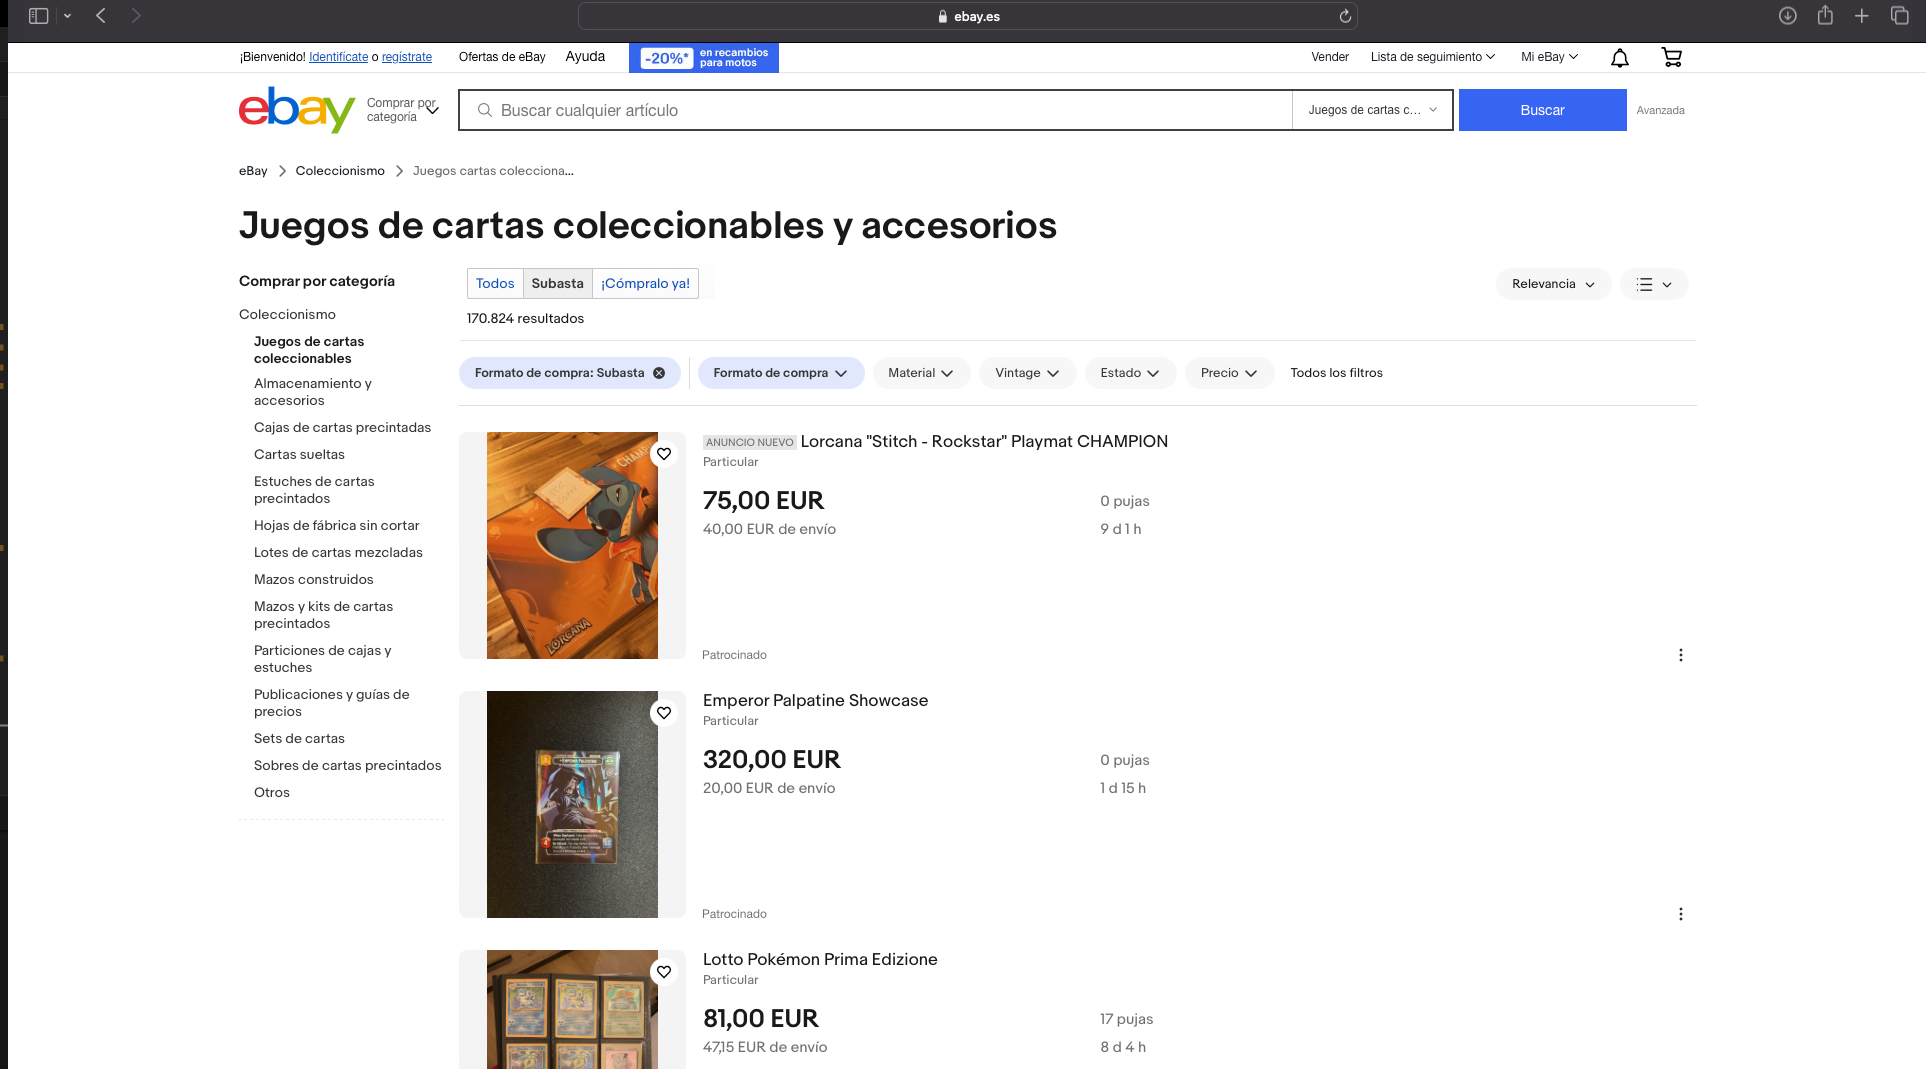
\includegraphics[width=0.9\textwidth]{figures/4-Estudio-viabilidad/4_Ebay.png}
    \caption{Página de subastas de la sección de coleccionismo de cartas de eBay}
    \label{fig:ebay}
    \hypertarget{fig:ebay}{}
\end{figure} 

\subsubsubsection{Ventajas de eBay}
Dentro del marco de LaLiga Fantasy, se destacan las siguientes características:
\begin{itemize}
    \item Para cada producto subastado, la plataforma ofrece la posibilidad de visualizar información detallada que incluye el número de pujas, la cantidad de pujadores, las retractaciones, el tiempo restante en la subasta, y proporciona un historial completo de las pujas realizadas en ese producto. Este historial incluye datos relevantes sobre las pujas, como su valor y la fecha en la que se efectuaron. Además, se brinda acceso a información pertinente sobre los pujadores involucrados.
    \item eBay proporciona a los usuarios la capacidad de configurar pujas automáticas. En este proceso, el comprador define el precio máximo que está dispuesto a pagar por el producto, y la plataforma aumenta automáticamente la oferta en su nombre, siempre que sea necesario, para mantener al comprador como el principal postor hasta alcanzar el límite previamente establecido.
    \item Los usuarios tienen la posibilidad de examinar el perfil del vendedor, explorar otros productos que este tenga en venta y establecer contacto directo con él.
    \item Como vendedor, la plataforma te brinda la capacidad de definir el valor inicial de la puja, decidir si deseas recibir ofertas, establecer la fecha de inicio de la subasta, determinar su duración y habilitar la opción de compra directa a un precio específico de tu elección.
\end{itemize}

\subsubsubsection{Desventajas de eBay}
A continuación, es posible señalar las siguientes desventajas:
\begin{itemize}
    \item La interfaz de usuario muestra una gran cantidad de información, lo que puede resultar confuso para alguien que no está acostumbrado a ella.
    \item Cuando se va a realizar una puja, no aparece una ventana emergente de confirmación de puja o similar por lo que es fácil introducir una puja errónea y, posteriormente, puede resultar complicado retirarla.
    \item Las subastas tienen incrementos de puja predefinidos, lo que significa que no puedes especificar un valor concreto por el que desees pujar.
\end{itemize}

\subsubsubsection{Ventajas del nuevo sistema respecto eBay}
\begin{itemize}
    \item El sistema en desarrollo presentará una interfaz simple e intuitiva, que proporcionará todos los datos esenciales para efectuar una puja con confianza, sin abrumar al usuario con una sobrecarga de información.
    \item El sistema que se desarrollará proporcionará al usuario información sobre las condiciones para retirar una puja antes de su confirmación.
\end{itemize}

% datos de facturación de laliga y juegos fantasy
% https://www.palco23.com/entorno/los-fantasy-se-preparan-para-su-boom-el-negocio-rebasara-416-millones-en-2024
% ebay https://www.ebayinc.com/company/

\section{Valoración de alternativas de solución}

En el presente apartado, se realiza un examen detallado de las diversas alternativas tecnológicas y arquitectónicas disponibles que satisfacen los requisitos previamente establecidos para el proyecto. 

Este análisis implica una evaluación rigurosa de las ventajas y desventajas asociadas a cada opción. La finalidad es identificar la solución más apropiada que no solo cumpla con los requisitos funcionales y no funcionales del proyecto, sino que también se alinee óptimamente con las restricciones y objetivos globales del mismo.

\subsection{Valoración de alternativas para la arquitectura}
A continuación, se presenta una comparación de varias alternativas arquitectónicas para el desarrollo del sistema.
\subsubsection{Arquitectura Monolítica}
La arquitectura monolítica es un enfoque de desarrollo de software en el que una aplicación se construye como una sola unidad. En este caso, todos los componentes del sistema se diseñan y se implementan como un único bloque, que se ejecuta como un único proceso.
Este enfoque en un proyecto pequeño puede ser beneficioso, ya que simplifica el proceso de desarrollo y sobretodo de despliegue. Sin embargo, a medida que el proyecto crece, la arquitectura monolítica se vuelve cada vez más compleja y difícil de mantener. Además, la escalabilidad de la aplicación se ve limitada por la necesidad de escalar el sistema en su conjunto, en lugar de poder escalar componentes individuales de forma independiente.
\begin{figure}[H]
    \centering
    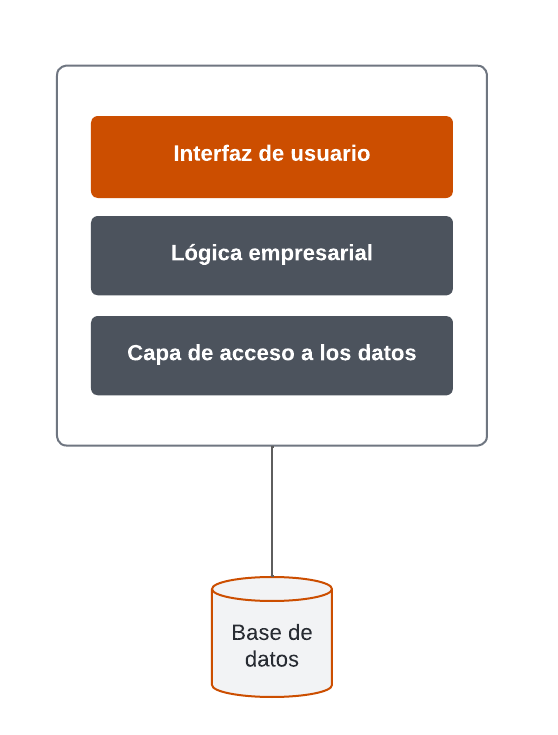
\includegraphics[width=0.4\textwidth]{figures/4-Estudio-viabilidad/4_Monolitica.png}
    \caption{Arquitectura Monolítica}
    \label{fig:arquitectura_monolitica}
    \hypertarget{fig:arquitectura_monolitica}{}
\end{figure}

\subsubsection{Arquitectura de Microservicios}
La arquitectura de microservicios es un enfoque de desarrollo de software en el que una aplicación se construye como un conjunto de servicios pequeños, independientes y altamente escalables. Cada servicio se ejecuta como un proceso separado y se comunica con otros servicios mediante mecanismos ligeros, como una API REST.
Este enfoque permite que los servicios se desarrollen, desplieguen y escalen de forma independiente, lo que facilita la gestión de proyectos complejos. Sin embargo, la arquitectura de microservicios también introduce una mayor complejidad en el desarrollo y la gestión de la aplicación, ya que requiere la implementación de mecanismos de comunicación entre los servicios, así como la gestión de la escalabilidad de cada uno de ellos.
\begin{figure}[H]
    \centering
    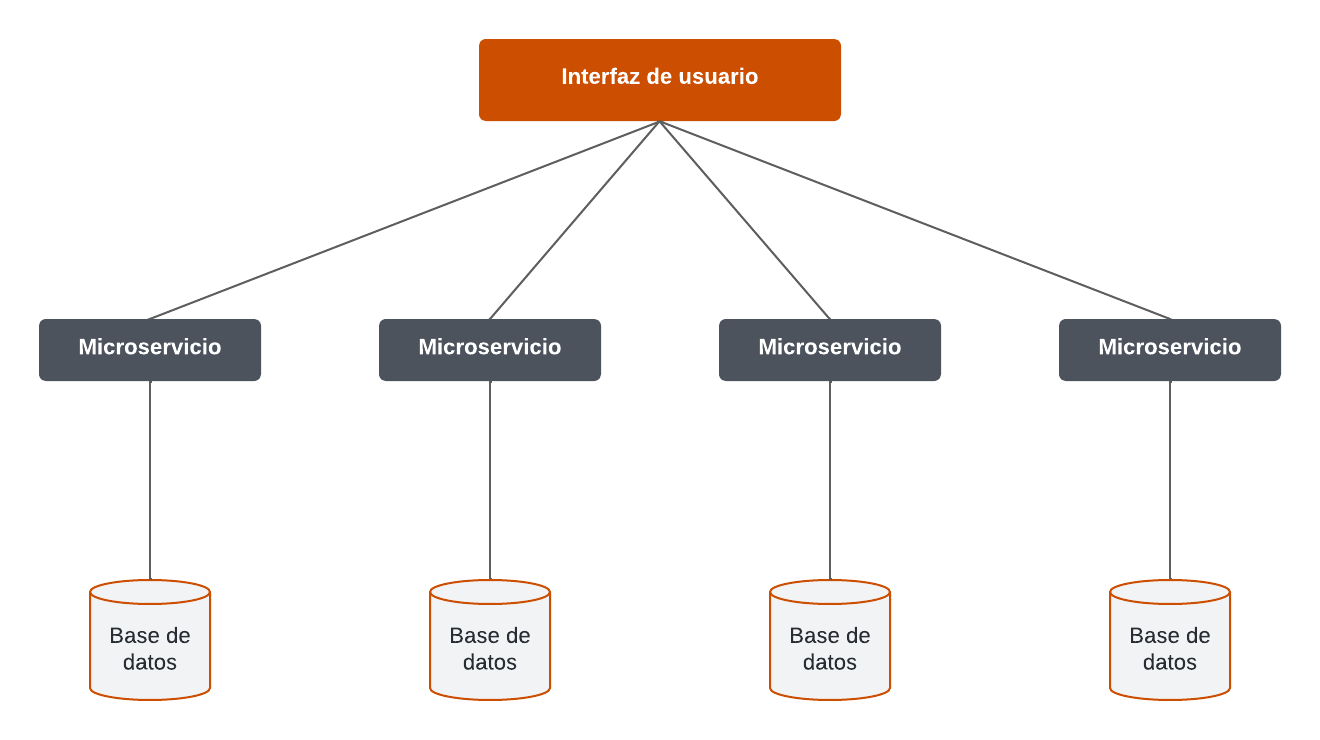
\includegraphics[width=0.7\textwidth]{figures/4-Estudio-viabilidad/4_Microservicios.png}
    \caption{Arquitectura de Microservicios}
    \label{fig:arquitectura_microservicios}
    \hypertarget{fig:arquitectura_microservicios}{}
\end{figure}

\subsubsection{Arquitectura de REST API y WepApp}    
Se caracteriza por una clara división entre cliente y servidor, encapsulados respectivamente en WepApp (frontend) y REST API (backend). Esta separación promueve una organización modular, facilitando el mantenimiento del proyecto al separar de forma clara las distintas responsabilidades. 
Este enfoque es un punto intermedio entre las dos arquitecturas anteriores, ya que permite una mayor flexibilidad en el desarrollo y la gestión de la aplicación, sin introducir una complejidad excesiva. 
\begin{figure}[H]
    \centering
    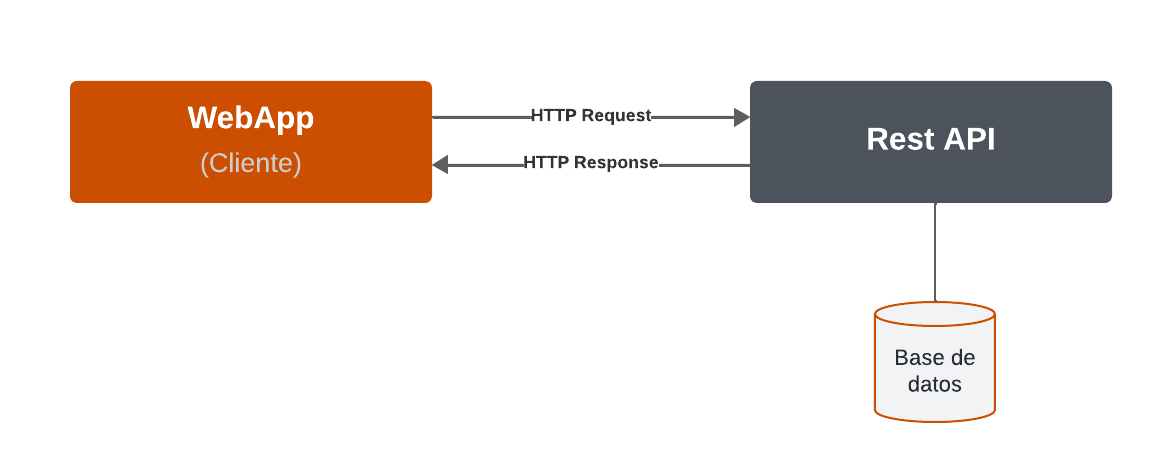
\includegraphics[width=0.7\textwidth]{figures/4-Estudio-viabilidad/4_WebApp_RestApi.png}
    \caption{Arquitectura de REST API y WebApp}
    \label{fig:arquitectura_rest_api_webapp}
    \hypertarget{fig:arquitectura_rest_api_webapp}{}
\end{figure}

\subsubsection{Comparativa de alternativas arquitectónicas}
Mediante la siguiente tabla, se presenta una comparación de las alternativas arquitectónicas previamente mencionadas.

\begin{table}[htb]
    \centering
    \caption{Comparación de Arquitecturas de Software}
    \label{tabla:comparacion_arquitecturas}
    \hypertarget{table:comparacion_arquitecturas}{}
    \begin{tabular}{
       >{\columncolor{rowcolor}\raggedright\arraybackslash}p{4cm}
       >{\raggedright\arraybackslash}p{3cm}
       >{\raggedright\arraybackslash}p{3cm}
       >{\raggedright\arraybackslash}p{3cm} }
    \rowcolor{lightgreen}
    \toprule
    \textbf{Criterio} & \textbf{Arquitectura Monolítica} & \textbf{Arquitectura de Microservicios} & \textbf{API REST y WebApp} \\
    \midrule
    Complejidad Inicial & Baja & Alta & Moderada \\
    \midrule
    Escalabilidad & Limitada & Alta & Moderada \\
    \midrule
    Facilidad de Mantenimiento & Alta en proyectos pequeños & Moderada a baja & Moderada si cada módulo tiene una estructura interna clara \\
    \midrule
    Despliegue & Sencillo & Complejo & Moderado \\
    \midrule
    Gestión de Proyectos & Simple en proyectos pequeños & Requiere coordinación compleja & Balanceada \\
    \midrule
    Independencia de Componentes & No & Sí & Parcial \\
    \midrule
    Adaptabilidad a Cambios & Baja & Alta & Moderada \\
    \midrule
    Recomendado para & Proyectos pequeños y simples & Proyectos grandes y escalables & Proyectos con necesidad de separación clara entre frontend y backend \\
    \bottomrule
    \end{tabular}
\end{table}


\subsubsection{Decisión final de la arquitectura}
Tras un análisis exhaustivo de las alternativas disponibles, se ha optado por implementar una arquitectura de API REST y WebApp.

Esta decisión permite alcanzar un equilibrio entre la simplicidad inherente a la arquitectura monolítica y la escalabilidad ofrecida por la arquitectura de microservicios. Además, esta elección facilita la gestión del proyecto mediante una separación clara entre el frontend y el backend. Tal distinción posibilita el desarrollo y despliegue independiente de cada componente, contribuyendo a la minimización de riesgos asociados a fallos en cadena. 
Además, cada módulo, operando de manera aislada, mejora significativamente la disponibilidad y confiabilidad del sistema.



\subsection{Valoración de alternativas para el Backend}
Es crucial seleccionar una tecnología de backend que no solo soporte eficientemente las operaciones en tiempo real sino que también se integre de manera óptima con el frontend.
A continuación, se presenta un análisis de varias alternativas para el desarrollo del backend teniendo en cuenta estos requisitos.

\subsubsection{Java con Spring Boot}
\coloredUnderline{\href{https://www.java.com/es/}{Java}} es un lenguaje de programación orientado a objetos que destaca por su portabilidad y robustez, siendo ampliamente utilizado en el desarrollo de aplicaciones empresariales. 
La combinación con \coloredUnderline{\href{https://spring.io/projects/spring-boot}{Spring Boot}} permite un desarrollo ágil con una amplia gama de herramientas como Spring Data y Spring Security entre otras. 
Entre sus ventajas, además de las herramientas mencionadas, destacan su escalabilidad, su robustez en el manejo de transacciones y su amplia comunidad. 
Sin embargo, Java con Spring Boot presenta una curva de aprendizaje significativa y, aunque Spring Boot puede manejar aplicaciones en tiempo real mediante Spring WebFlux, su rendimiento en este ámbito puede ser inferior comparado con otras tecnologías. Además, la integración con el frontend, podría no ser la más rápida en términos de desarrollo.

\subsubsubsection{Node.js con Express}
\coloredUnderline{\href{https://nodejs.org/es/}{Node.js}} es un entorno de ejecución para JavaScript en el lado del servidor, conocido por su modelo de I/O no bloqueante y su eficiencia en el manejo de múltiples conexiones simultáneas
La integración de Node.js con \coloredUnderline{\href{https://expressjs.com/es/}{Express}}, un framework ligero y flexible, ofrece una solución óptima para desarrollar aplicaciones web dinámicas.
Esta combinación destaca por su capacidad para gestionar operaciones en tiempo real de manera eficiente y su sinergia natural con tecnologías frontend basadas en JavaScript, facilitando un desarrollo cohesivo y ágil entre el backend y el frontend.
Como desventajas, cabe mencionar que Node.js puede no ser la opción más adecuada para tareas que requieren un alto uso de CPU debido a su naturaleza de ejecución de un solo hilo, ya que su rendimiento en este ámbito puede ser inferior al de otras tecnologías.

\subsubsection{Python con Django}
\coloredUnderline{\href{https://www.python.org/}{Python}}, un lenguaje de programación de alto nivel, se caracteriza por su versatilidad y amplia gama de bibliotecas. Utilizado ampliamente en 
aplicaciones empresariales combinado con \coloredUnderline{\href{https://www.djangoproject.com/}{Django}}, un framework de alto nivel que se enfoca en el desarrollo rápido y eficiente.
Como ventajas, destacan su desarrollo rápido, sus excelentes capacidades de seguridad y su buena documentación.
Aunque Django puede ser configurado para soportar aplicaciones en tiempo real mediante Django Channels, su rendimiento en estos escenarios puede no ser tan óptimo como el de Node.js. Además, aunque Django asegura una buena integración con el frontend, puede no ser la opción más ágil para aplicaciones que requieren una interacción constante.



\subsubsection{Comparativa de alternativas para el Backend}
En la siguiente tabla, se presenta una comparación de las alternativas para el desarrollo del Backend.
\begin{table}[H]
    \centering
    \begin{tabular}{ 
       >{\columncolor{rowcolor}\raggedright\arraybackslash}p{3cm} 
       >{\raggedright\arraybackslash}p{3cm} 
       >{\raggedright\arraybackslash}p{3cm} 
       >{\raggedright\arraybackslash}p{3cm} }
        \rowcolor{lightgreen}
    \toprule
    \textbf{Criterio} & \textbf{Java con Spring Boot} & \textbf{Node.js con Express} & \textbf{Python con Django} \\
    \midrule
    \textbf{Modelo de Programación} & Orientado a objetos, con énfasis en inyección de dependencias. & Basado en eventos y callbacks. & Orientado a componentes/modelos con énfasis en la reutilización de código. \\
    \midrule
    \textbf{Funcionalidad en tiempo real} & Buen manejo de transacciones pero menos óptimo para tiempo real. & Excelente para operaciones en tiempo real gracias a su eficiencia en I/O. & Posible pero requiere más configuración para tiempo real. \\
    \midrule
    \textbf{Integración con Frontend} & Buena, puede requerir esfuerzos adicionales. & Natural y fluida. & Buena, pero puede necesitar configuraciones extra. \\
    \midrule
    \textbf{Escalabilidad} & Alta, pero con escalabilidad vertical. & Alta, con facilidad para escalar horizontalmente. & Moderada, con algunas limitaciones en escalabilidad. \\
    \midrule
    \textbf{Seguridad} & Fuertes capacidades de seguridad. & Requiere implementaciones adicionales para seguridad. & Seguridad integrada y robusta. \\
    \bottomrule
    \end{tabular}
    \caption{Comparación de Tecnologías para el Backend}
    \label{tabla:comparacion_backend}
    \hypertarget{table:comparacion_backend}{}
    \end{table}

    
\subsubsection{Decisión final del Backend}
Considerando las necesidades del sistema a desarrollar, para soportar subastas en tiempo real y una integración fluida con el frontend la opción más adecuada es Node.js con Express.


\subsection{Valoración de alternativas para el Frontend}
A continuación, se presenta un análisis de alternativas para el desarrollo del frontend.

\subsubsection{React}
\coloredUnderline{\href{https://es.react.dev}{React}} es una biblioteca de JavaScript desarrollada y mantenida por Facebook, centrada en la construcción de interfaces de usuario a través de componentes reutilizables. Se caracteriza por su virtual DOM y su enfoque declarativo.

Entre sus ventajas, destacan su amplia comunidad, su rendimiento optimizado con Virtual DOM y su flexibilidad en la elección de estilos y componentes. 
Como desventajas cabe mencionar las actualizaciones frecuentes que implican mantenerse al día con los cambios y que necesita integración con otras herramientas para ser una solución completa.


\subsubsection{Angular}
\coloredUnderline{\href{https://angular.io/}{Angular}} es un framework de desarrollo web mantenido por Google, conocido por su enfoque en aplicaciones de página única (SPA). Utiliza TypeScript como lenguaje principal y proporciona un entorno robusto y completo para el desarrollo.

Entre sus ventajas, destaca su ecosistema completo, promueve un estilo de desarrollo coherente y mantenible y, además, cuenta con una comunidad activa y un amplio soporte de Google, lo que garantiza actualizaciones y soporte continuo.
Sin embargo, Angular puede ser excesivo para proyectos pequeños, ya que su curva de aprendizaje es pronunciada y su configuración inicial puede ser compleja.

\subsubsection{Vue.js}
\coloredUnderline{\href{https://vuejs.org/}{Vue.js}} es un framework progresivo para la construcción de interfaces de usuario, creado por Evan You. Se destaca por su facilidad de adopción, su sistema reactividad y su enfoque en la simplicidad.

Entre sus ventajas, destacan su sintaxis sencilla, su buena documentación y su facilidad de integración en proyectos existentes.
Aunque su uso va en aumento, su comunidad es más pequeña en comparación con React o Angular, lo que se traduce en menos librerías y recursos disponibles.

\subsubsection{Comparativa de alternativas para el Frontend}
A continuación, se presenta una comparación de las alternativas para el desarrollo del Frontend.

\begin{table}[H]
    \centering
    \begin{tabular}{ 
       >{\columncolor{rowcolor}\raggedright\arraybackslash}p{2.5cm} 
       >{\raggedright\arraybackslash}p{3.5cm} 
       >{\raggedright\arraybackslash}p{3.5cm} 
       >{\raggedright\arraybackslash}p{3.5cm} }
        \rowcolor{lightgreen}
    \toprule
    
    \textbf{Criterio} & \textbf{React} & \textbf{Angular} & \textbf{Vue.js} \\
    \midrule
    \textbf{Velocidad y Rendimiento} & Alto con Virtual DOM. Optimizado para cambios dinámicos de UI. & Buen rendimiento, pero puede ser más lento en proyectos grandes debido a su complejidad. & Rendimiento similar a React, con optimizaciones en la actualización de la UI. \\
    \midrule
    \textbf{Mantener el Estado} & Requiere bibliotecas adicionales como Redux para manejo complejo del estado. & Gestión de estado integrada, adecuada para aplicaciones complejas. & Sistema reactividad sencillo, para manejo de estado complejo requiere la biblioteca Vuex. \\
    \midrule
    \textbf{Comunidad} & Muy grande y activa, con un ecosistema extenso. & Amplia y soportada por Google, con muchas empresas adoptándolo. & Creciente y entusiasta, con un enfoque en la facilidad de uso. \\
    \midrule
    \textbf{Curva de Aprendizaje} & Moderada; JSX y el ecosistema pueden requerir tiempo de aprendizaje. & Elevada; TypeScript y su arquitectura completa requieren más tiempo para aprender. & Baja; Vue es considerado fácil de aprender, especialmente para principiantes. \\
    \midrule
    \textbf{Escalabilidad} & Muy escalable con un enfoque modular y reutilizable. & Diseñado para aplicaciones empresariales escalables y complejas. & Escalable, pero más adecuado para proyectos de tamaño mediano. \\
    \midrule
    \textbf{Ecosistemas y Módulos} & Rico ecosistema con una gran cantidad de módulos y herramientas. & Ecosistema completo con soluciones integradas para muchas necesidades. & Ecosistema más pequeño aunque en crecimiento, con módulos y librerías en aumento. \\
    \bottomrule
    \end{tabular}
    \caption{Análisis Comparativo de Frameworks y Bibliotecas de Frontend}
    \label{tabla:comparacion_frontend}
    \hypertarget{table:comparacion_frontend}{}
\end{table}

\subsubsection{Decisión final del Frontend}
Tras una evaluación detallada de las distintas opciones disponibles y en función de los requisitos específicos del sistema a desarrollar, se ha determinado que React es la tecnología más adecuada para el frontend.

Esta decisión se basa, principalmente, en la gran comunidad de React y en la rica colección de recursos disponles.

\subsection{Valoración de alternativas para la Base de Datos}
Por último, se presenta un análisis de alternativas para la base de datos del sistema.

\subsubsection{MySQL}
\coloredUnderline{\href{https://www.mysql.com/}{MySQL}} es un sistema de gestión de bases de datos relacional de código abierto, ampliamente utilizado en aplicaciones web. 

Entre sus ventajas, destacan su amplia adopción lo que conlleva una gran cantidad de recursos y documentación disponibles, su fiabilidad y robustez y su facilidad de uso. 

Por otro lado, MySQL puede no ser la opción más adecuada para aplicaciones que requieren de operaciones avanzadas de análisis y procesamiento de datos, ya que su rendimiento en este ámbito puede ser inferior al de otras bases de datos.

\subsubsection{MongoDB}
\coloredUnderline{\href{https://www.mongodb.com/}{MongoDB}} es una base de datos NoSQL orientada a documentos, diseñada para la escalabilidad y la flexibilidad. Se caracteriza por su capacidad para manejar grandes volúmenes de datos y su esquema flexible.

Entre sus ventajas, destacan su flexibilidad, permite que la base de datos crezca con la aplicación añadiendo nuevos campos a los documentos.
Además, MongoDB es altamente escalable y puede manejar grandes volúmenes de datos de manera eficiente.

Sin embargo, MongoDB puede no ser la opción más adecuada para aplicaciones que requieren transacciones ACID complejas, ya que su modelo de consistencia eventual puede no ser adecuado para todas las aplicaciones.

\subsubsection{PostgreSQL}
\coloredUnderline{\href{https://www.postgresql.org/}{PostgreSQL}} es un sistema de gestión de bases de datos relacional de código abierto y gratuito, conocido por su robustez, escalabilidad y soporte para transacciones ACID.

Entre sus ventajas, destacan su cumplimiento con los estándares SQL, su soporte para transacciones ACID y su capacidad para manejar grandes volúmenes de datos asegurando la integridad y seguridad de los mismos.

Como inconvenientes, cabe mencionar que PostgreSQL puede ser más lento que otras bases de datos en operaciones de lectura y escritura para bases de datos pequeñas ya que está enfocada en manejar un gran volumen de datos,
 y su curva de aprendizaje puede ser pronunciada para usuarios no familiarizados con SQL.

\subsubsection{Comparativa de alternativas para la Base de Datos}
En la siguiente tabla, se presenta una comparación de las alternativas para la base de datos del sistema.
\begin{table}[H]
    \centering
    \begin{tabular}{ 
       >{\columncolor{rowcolor}\raggedright\arraybackslash}p{3cm} 
       >{\raggedright\arraybackslash}p{3cm} 
       >{\raggedright\arraybackslash}p{3cm} 
       >{\raggedright\arraybackslash}p{3cm} }
        \rowcolor{lightgreen}
    \toprule
    \textbf{Criterio} & \textbf{MySQL} & \textbf{MongoDB} & \textbf{PostgreSQL} \\
    \midrule
    \textbf{Tipo de Base de Datos} & Relacional & NoSQL & Relacional \\
    \midrule
    \textbf{Modelo de Datos} & Tablas y Filas & Documentos JSON/BSON & Tablas y Filas \\
    \midrule
    \textbf{Lenguaje de Consulta} & SQL & MongoDB Query Language (MQL) & SQL \\
    \midrule
    \textbf{Escalabilidad} & Escalabilidad vertical y soporte para horizontal & Escalabilidad horizontal mediante sharding & Escalabilidad vertical y horizontal \\
    \midrule
    \textbf{Transacciones} & Soporte completo de ACID & Soporte parcial de ACID en ciertas operaciones & Soporte completo de ACID \\
    \midrule
    \textbf{JSON} & Soporte limitado mediante campos JSON & JSON nativo & Soporte avanzado de JSON y JSONB \\
    \midrule
    \textbf{Flexibilidad de Esquema} & Esquemas rígidos & Esquemas flexibles& Esquemas rígidos \\
    \midrule
    \textbf{Rendimiento} & Alto rendimiento en lecturas & Alto rendimiento en escrituras & Alto rendimiento en lecturas y escrituras \\
    \bottomrule
    \end{tabular}
    \caption{Comparativa entre MySQL, MongoDB y PostgreSQL}
    \label{tabla:comparacion_bases_datos}
    \hypertarget{table:comparacion_bases_datos}{}
\end{table}


\subsubsection{Decisión final de la Base de Datos}
Tras un análisis detallado de las distintas opciones disponibles y en función de los requisitos específicos del sistema a desarrollar, se ha determinado que MongoDB es la tecnología más adecuada para la base de datos. 

Esta elección se basa en un \textit{trade-off}, es decir, se acepta la falta de integridad referencial y la consistencia eventual a cambio de una mayor flexibilidad y escalabilidad en el manejo de datos que es lo que se necesita para el sistema a desarrollar.


\subsection{Selección final de alternativas de solución}

Se han seleccionado las siguientes tecnologías como alternativas de solución: Node.js con Express para el backend, React.js para el frontend, y MongoDB como base 
de datos. 

Estas decisiones conforman una arquitectura \textbf{MERN} (MongoDB, Express, React, Node.js), ejemplificada en la \coloredUnderline{\hyperlink{fig:arquitectura_mern}{Figura \ref*{fig:arquitectura_mern}: \nameref*{fig:arquitectura_mern}}}. 

Esta arquitectura presenta diversas ventajas, tales como la familiaridad de los desarrolladores con las tecnologías involucradas, el amplio soporte y documentación disponibles debido a su uso común en el desarrollo de aplicaciones web actuales,
y la facilidad de integración entre las tecnologías.

Se puede consultar más información sobre la arquitectura MERN en el siguiente enlace: \coloredUnderline{\href{https://www.mongodb.com/resources/languages/mern-stack}{MERN Stack}}.

\begin{figure}[H]
    \centering
    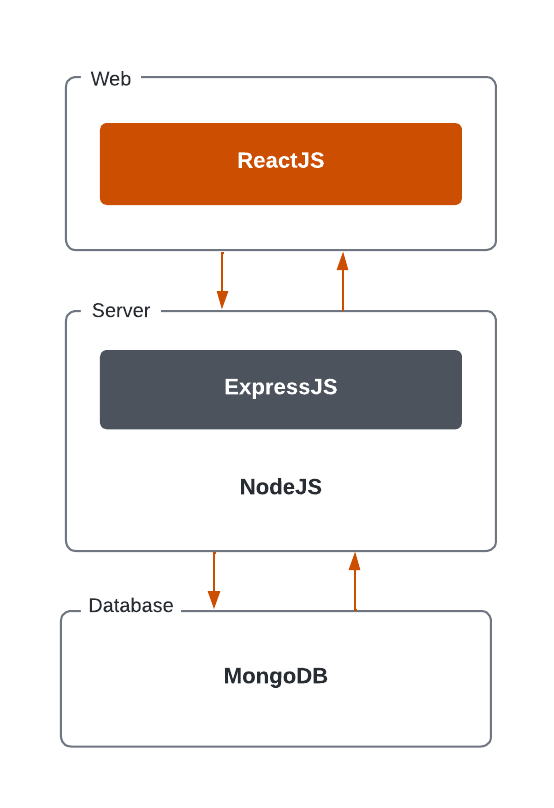
\includegraphics[width=0.4\textwidth]{figures/4-Estudio-viabilidad/4_MERN2.png}
    \caption{MERN Stack: MongoDB, Express, React, Node.js}
    \label{fig:arquitectura_mern}
    \hypertarget{fig:arquitectura_mern}{}
\end{figure}



\newpage
\chapter{PLANIFICACIÓN Y GESTIÓN DEL TFG}
\noindent\begin{tikzpicture}
% Definir el degradado
\shade[left color=darkgreen, right color=lightgreen] (0,0) rectangle (\textwidth-1pt,0.2);

\end{tikzpicture}
\newpage
\section{PLANIFICACIÓN DEL PROYECTO}
En este apartado se abordará la planificación inicial del proyecto, detallando los aspectos más relevantes del mismo. 
Se incluirá la identificación de interesados, las tareas a realizar, la estructura de desglose de trabajo, la planificación temporal, los riesgos identificados y el presupuesto inicial.

\subsection{Identificación de Interesados}
Los interesados en el proyecto son las personas o grupos que pueden afectar o verse afectados por el proyecto. 
En el caso de este proyecto, los interesados son los siguientes:
\begin{itemize}
    \item \textbf{Usuarios:} Compradores de sobres, vendedores en subastas, pujadores y coleccionistas. Su satisfacción y experiencia de usuario son críticas para el éxito de la plataforma.
    \item \textbf{Desarrolladores:} Equipo encargado del desarrollo, mantenimiento y actualización de la plataforma.
    \item \textbf{Propietarios/Creadores:} Fundadores y administradores del proyecto, responsables de la visión, dirección y toma de decisiones estratégicas.
    \item \textbf{Inversores:} Personas o entidades que financian el proyecto, con expectativas de retorno sobre su inversión. Su interés reside en la rentabilidad y sostenibilidad del negocio.
    \item \textbf{Proveedores:} Proveedores de servicios tecnológicos y de infraestructura, como \textit{hosting}, sistemas de pago y seguridad.
    \item \textbf{Comunidades:} Grupos y foros de fans y coleccionistas de Pokémon que pueden influir en la popularidad y adopción de la plataforma. Su participación y \textit{feedback} pueden guiar mejoras y nuevas características.
    \item \textbf{Reguladores:} Entidades gubernamentales y de la industria que aseguran el cumplimiento de leyes y regulaciones aplicables al comercio digital y la protección de datos.
\end{itemize}


\subsection{OBS y PBS}
El OBS, \textit{Organizational Breakdown Structure} es una estructura que representa las responsabilidades sobre la realización de las tareas del proyecto. 
Por otro lado, el PBS  \textit{(Product Breakdown Structure)} es una estructura jerárquica que descompone el proyecto en los productos que se deben entregar para cumplir con los objetivos del proyecto.

\subsubsection{OBS} \label{sec:5-OBS}
\hypertarget{sec:5-OBS}{}
En este proyecto, se simulará una pequeña empresa ficticia para su realización. 
Se han identificado los distintos perfiles que intervienen en el proyecto, así como las tareas que cada uno debe realizar. 
Aunque el proyecto se llevará a cabo de forma individual, se ha considerado necesario estructurar estos roles para poder asignar un presupuesto adecuado a cada función.

Los roles identificados se especifican en \coloredUnderline{\hyperlink{table:obs}{Tabla: \ref*{table:obs} \nameref*{table:obs}}}. 
Cabe destacar que el rol de Jefe de Proyecto (JP) es el encargado de supervisar y coordinar el trabajo de los demás roles y este rol ha sido considerado tanto para el alumno como para el tutor del TFG.


\begin{table}[H]
\centering
\hypertarget{table:obs}{}
\caption{OBS (Organizational Breakdown Structure)}
\label{table:obs}
\begin{tabular}{>{\columncolor{lightgreen!20}}p{7cm} p{10cm}}
\toprule
\rowcolor{darkgreen!50}
\textbf{Abreviatura} & \textbf{Rol} \\
\midrule
JP & Jefe de Proyecto \\
\midrule
AN & Analista junior\\
\midrule
DI & Diseñador junior \\
\midrule
DS & Desarrollador de Software junior\\
\midrule
TE & Tester junior \\
\midrule
DOC & Documentador técnico \\
\bottomrule
\end{tabular}
\end{table}
 
Se ha decidido realizar una matriz de asignación de responsabilidades RACI para relacionar las tareas identifcadas en \coloredUnderline{\hyperlink{sec:5-WBS}{\ref*{sec:5-WBS} \nameref*{sec:5-WBS}}} con cada rol.
En esta matriz, a cada tarea se le asigna un rol con una de las siguientes responsabilidades:
\begin{itemize}
    \item \textbf{R:} Responsable. Persona que realiza la tarea.
    \item \textbf{A:} Aprobador. Persona que aprueba la tarea.
    \item \textbf{C:} Consultado. Persona a la que se consulta sobre la tarea.
    \item \textbf{I:} Informado. Persona a la que se informa sobre el avance y los resultados de la tarea.
\end{itemize}
Un mismo recursos puede tener varias responsabilidades en una misma tarea, en tal caso se anotarán separadas por el caracter \textit{``/''}.

\subsubsubsection{Análisis del proyecto}
En la \coloredUnderline{\hyperlink{table:matriz-analisis}{Tabla: \ref*{table:matriz-analisis} \nameref*{table:matriz-analisis}}} se muestra la matriz de responsabilidades para la fase de análisis.
\begin{table}[H]
    \centering
    \caption{Matriz RACI. Análisis del proyecto}
    \label{table:matriz-analisis}
    \hypertarget{table:matriz-analisis}{}
    \begin{tabular}{
    >{\columncolor{lightgreen!20}}m{7cm} 
    >{\columncolor{white}}m{1cm} 
    >{\columncolor{white}}m{1cm} 
    >{\columncolor{white}}m{1cm} 
    >{\columncolor{white}}m{1cm} 
    >{\columncolor{white}}m{1cm} 
    >{\columncolor{white}}m{1cm}}
    \cmidrule(l){2-7}
    \rowcolor{darkgreen!50}
    \cellcolor{white} & \multicolumn{6}{c}{\textbf{Roles}} \\
    \midrule
    \rowcolor{lightgreen!20}
    \cellcolor{darkgreen!50}\textbf{Tarea} & \textbf{JP} & \textbf{AN} & \textbf{DI} & \textbf{DS} & \textbf{TE} & \textbf{DOC} \\
    \midrule
    Análisis del sistema & A & R &  & C &  &  \\
    \midrule
    Análisis de la arquitectura & A & R &  & C &  &  \\
    \midrule
    Análisis de la infraestructura & A & R &  & C &  &  \\
    \midrule
    Determinación del alcance de desarrollo & A & R & I & C & I & I \\
    \bottomrule
    \end{tabular}
\end{table}

\subsubsubsection{Seguimiento del proyecto}
En la \coloredUnderline{\hyperlink{table:matriz-seguimiento}{Tabla: \ref*{table:matriz-seguimiento} \nameref*{table:matriz-seguimiento}}} se muestra la matriz de responsabilidades para la fase de seguimiento.
\begin{table}[H]
    \centering
    \caption{Matriz RACI. Seguimiento del proyecto}
    \label{table:matriz-seguimiento}
    \hypertarget{table:matriz-seguimiento}{}
    \begin{tabular}{
    >{\columncolor{lightgreen!20}}m{7cm} 
    >{\columncolor{white}}m{1cm} 
    >{\columncolor{white}}m{1cm} 
    >{\columncolor{white}}m{1cm} 
    >{\columncolor{white}}m{1cm} 
    >{\columncolor{white}}m{1cm} 
    >{\columncolor{white}}m{1cm}}
    \cmidrule(l){2-7}
    \rowcolor{darkgreen!50}
    \cellcolor{white} & \multicolumn{6}{c}{\textbf{Roles}} \\
    \midrule
    \rowcolor{lightgreen!20}
    \cellcolor{darkgreen!50}\textbf{Tarea} & \textbf{JP} & \textbf{AN} & \textbf{DI} & \textbf{DS} & \textbf{TE} & \textbf{DOC} \\
    \midrule
    Reunión de arranque & A & I & I & I & I & R \\
    \midrule
    Reuniones periódicas & A & I & I & I & I & R\\
    \midrule
    Reunión de revisión & A & I & I & C & I & R  \\
    \midrule
    Reunión final & A & I & I & C & I & R  \\
    \bottomrule
    \end{tabular}
\end{table}

\subsubsubsection{Diseño del sistema}
En la \coloredUnderline{\hyperlink{table:matriz-diseno}{Tabla: \ref*{table:matriz-diseno} \nameref*{table:matriz-diseno}}} se presenta la matriz de responsabilidades correspondiente a la fase de diseño. 
Las tareas listadas en esta matriz son las tareas "hoja" de dicha fase, es decir, aquellas que no se descomponen en subtareas más pequeñas y, por lo tanto, representan las tareas finales 
de la fase de diseño.
\begin{table}[H]
    \centering
    \caption{Matriz RACI. Diseño del sistema}
    \label{table:matriz-diseno}
    \hypertarget{table:matriz-diseno}{}
    \begin{tabular}{
    >{\columncolor{lightgreen!20}}m{7cm} 
    >{\columncolor{white}}m{1cm} 
    >{\columncolor{white}}m{1cm} 
    >{\columncolor{white}}m{1cm} 
    >{\columncolor{white}}m{1cm} 
    >{\columncolor{white}}m{1cm} 
    >{\columncolor{white}}m{1cm}}
    \cmidrule(l){2-7}
    \rowcolor{darkgreen!50}
    \cellcolor{white} & \multicolumn{6}{c}{\textbf{Roles}} \\
    \midrule
    \rowcolor{lightgreen!20}
    \cellcolor{darkgreen!50}\textbf{Tarea} & \textbf{JP} & \textbf{AN} & \textbf{DI} & \textbf{DS} & \textbf{TE} & \textbf{DOC} \\
    \midrule
    \textit{Backend}. Diseño del módulo de usuarios & A &  & I & R &  &  I \\
    \midrule
    \textit{Backend}. Diseño del módulo de cartas & A &  & I & R &  & I \\
    \midrule
    \textit{Backend}. Diseño del módulo de sobres de cartas & A &  & I & R &  & I \\
    \midrule
    \textit{Backend}. Diseño del módulo de subastas & A &  & I & R &  & I \\
    \midrule
    \textit{Backend}. Diseño del módulo de transacciones & A &  & I & R &  & I \\
    \midrule
    \textit{Frontend}. Diseño de logo de la aplicación & A &  & R & I &  & I \\
    \midrule
    \textit{Frontend}. Diseño de la moneda de la aplicación & A &  & R & I &  & I \\
    \midrule
    \textit{Frontend}. Diseño de la temática & A &  & R & C/I &  & I \\
    \midrule
    \textit{Frontend}. Diseño del árbol de navegación & A &  & R & C/I &  & I \\
    \midrule
    \textit{Frontend}. Diseño de las páginas de información & A &  & R & C/I &  & I \\
    \midrule
    \textit{Frontend}. Diseño de las página \textit{Home} & A &  & R & C/I &  & I \\
    \midrule
    \textit{Frontend}. Diseño de las página de error & A &  & R & C/I &  & I \\
    \bottomrule
    \end{tabular}
\end{table}

\subsubsubsection{Implementación del sistema}
En la \coloredUnderline{\hyperlink{table:matriz-implementacion}{Tabla: \ref*{table:matriz-implementacion} \nameref*{table:matriz-implementacion}}} se muestra la matriz de responsabilidades para la fase de implementación.
\begin{table}[H]
    \centering
    \caption{Matriz RACI. Implementación del proyecto}
    \label{table:matriz-implementacion}
    \hypertarget{table:matriz-implementacion}{}
    \begin{tabular}{
    >{\columncolor{lightgreen!20}}m{7cm} 
    >{\columncolor{white}}m{1cm} 
    >{\columncolor{white}}m{1cm} 
    >{\columncolor{white}}m{1cm} 
    >{\columncolor{white}}m{1cm} 
    >{\columncolor{white}}m{1cm} 
    >{\columncolor{white}}m{1cm}}
    \cmidrule(l){2-7}
    \rowcolor{darkgreen!50}
    \cellcolor{white} & \multicolumn{6}{c}{\textbf{Roles}} \\
    \midrule
    \rowcolor{lightgreen!20}
    \cellcolor{darkgreen!50}\textbf{Tarea} & \textbf{JP} & \textbf{AN} & \textbf{DI} & \textbf{DS} & \textbf{TE} & \textbf{DOC} \\
    \midrule
    Reunión de arranque & A & I & I & I & I & R \\
    \midrule
    Reuniones periódicas & A & I & I & I & I & R\\
    \midrule
    Reunión de revisión & A & I & I & C & I & R  \\
    \midrule
    Reunión final & A & I & I & C & I & R  \\
    \bottomrule
    \end{tabular}
\end{table}

\subsubsection{PBS} \label{sec:5-PBS}
\hypertarget{sec:5-PBS}{}
El PBS, \textit{Product Breakdown Structure}, es una estructura jerárquica que descompone el proyecto en los productos que se deben entregar para cumplir 
con los objetivos del proyecto. 
En las siguientes secciones se detallan los productos que se deben entregar en el proyecto BidMon Universe.

\subsubsection{PBS. Visión general}
En la \coloredUnderline{\hyperlink{fig:5_PBS-Vision-General}{Figura \ref*{fig:5_PBS-Vision-General}: \nameref*{fig:5_PBS-Vision-General}}} se muestran los productos de alto nivel que se deben entregar en el proyecto BidMon Universe. 
En las siguientes secciones, se entrará en detalle en cada uno de los productos.

\begin{figure}[H]
    \hypertarget{fig:5_PBS-Vision-General}{}
    \centering
    \includegraphics[width=0.5\linewidth]{figures/5-PBS/5_PBS-Vision-General.png}
    \caption{PBS. Visión general}
    \label{fig:5_PBS-Vision-General}
\end{figure}


\subsubsection{PBS. Análisis del sistema}
En la \coloredUnderline{\hyperlink{fig:5_PBS-Analisis-Sistema}{Figura \ref*{fig:5_PBS-Analisis-Sistema}: \nameref*{fig:5_PBS-Analisis-Sistema}}}, se detallan los productos que se deben entregar en la fase de análisis del sistema.
\begin{figure}[H]
    \hypertarget{fig:5_PBS-Analisis-Sistema}{}
    \centering
    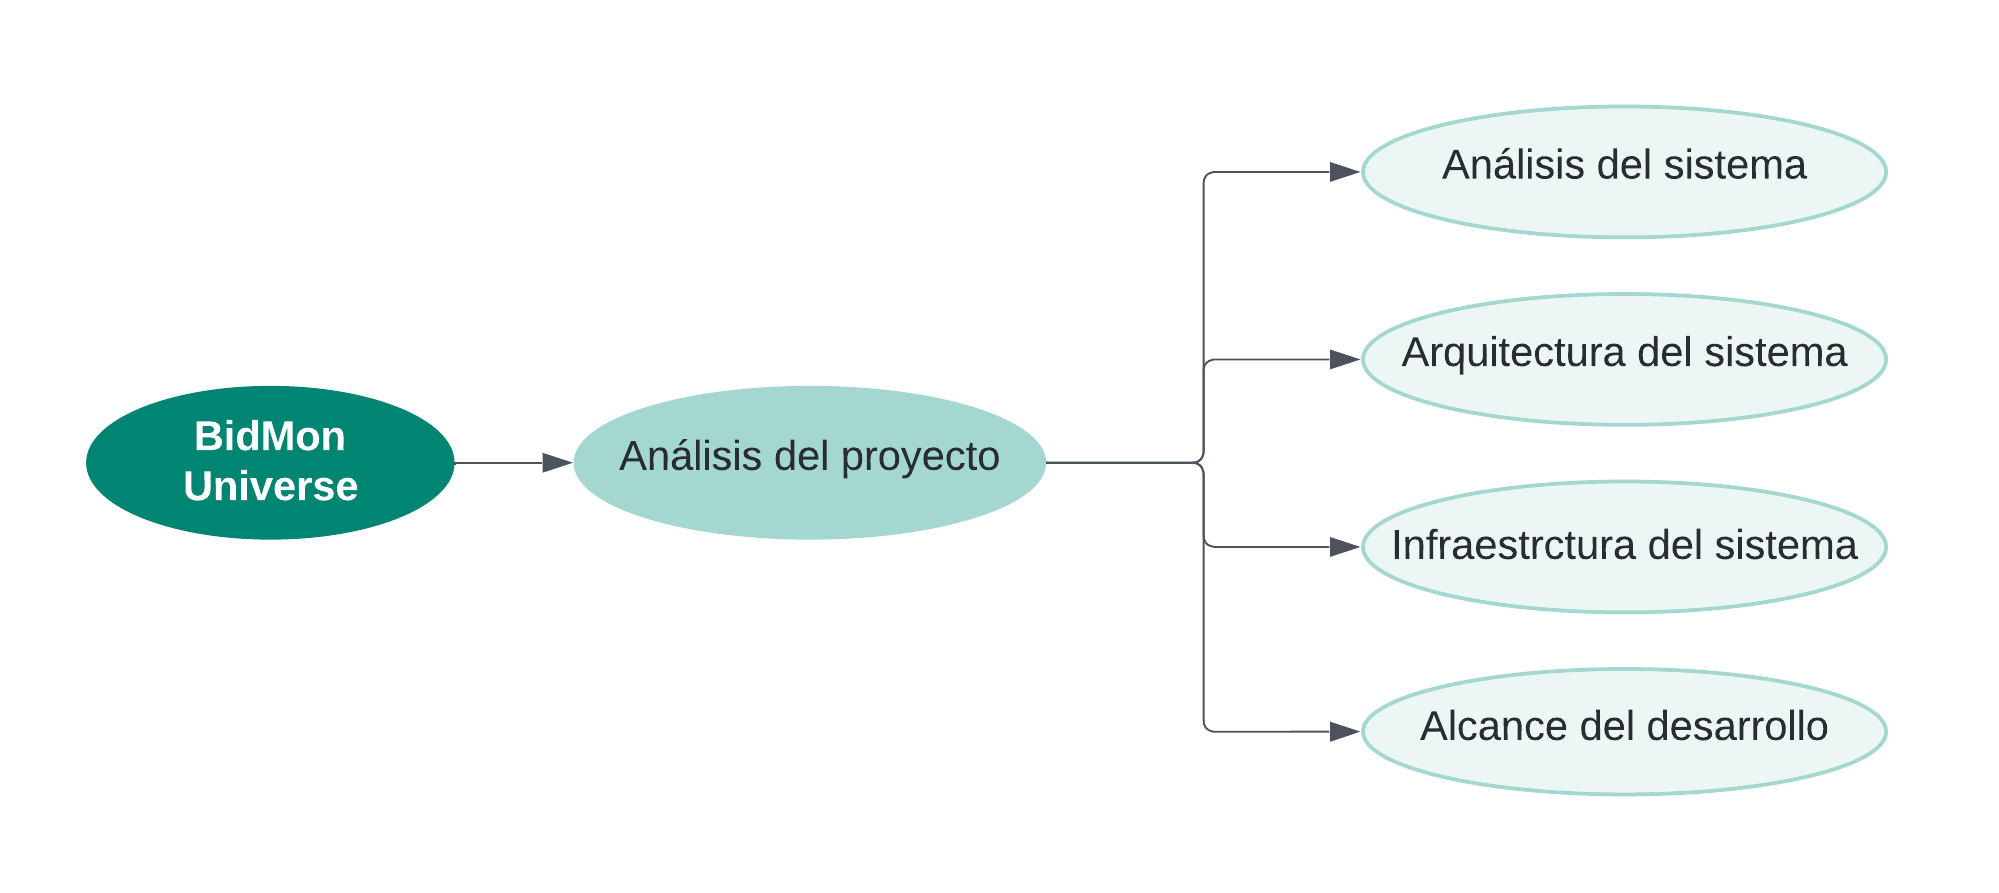
\includegraphics[width=0.7\linewidth]{figures/5-PBS/5_PBS-Analisis.png}
    \caption{PBS. Análisis del sistema}
    \label{fig:5_PBS-Analisis-Sistema}
\end{figure}

\subsubsection{PBS. Seguimiento del sistema}
En esta fase se detallan los productos que se obtienen en la fase de segumiento del proyecto, principalmente documentación e informes como se muestra en la \coloredUnderline{\hyperlink{fig:5_PBS-Seguimiento-Sistema}{Figura \ref*{fig:5_PBS-Seguimiento-Sistema}: \nameref*{fig:5_PBS-Seguimiento-Sistema}}}.
\begin{figure}[H]
    \hypertarget{fig:5_PBS-Seguimiento-Sistema}{}
    \centering
    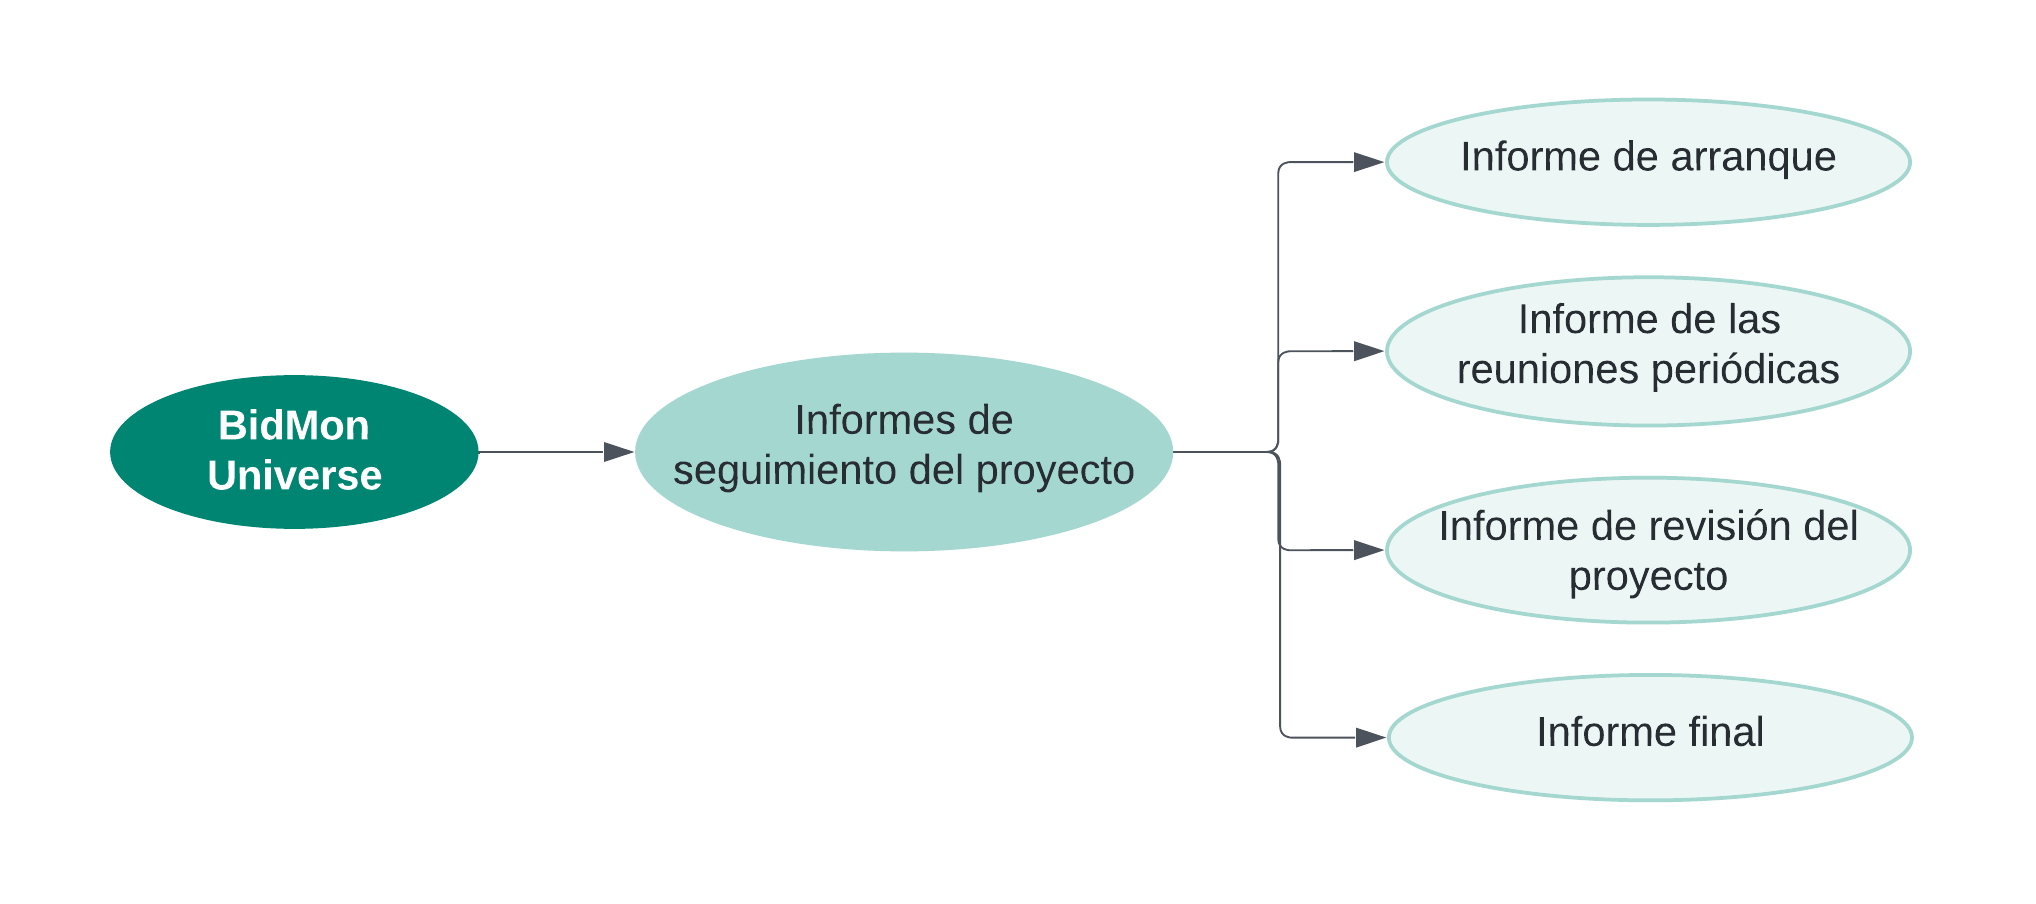
\includegraphics[width=0.7\linewidth]{figures/5-PBS/5_PBS-Seguimiento.png}
    \caption{PBS. Seguimiento del sistema}
    \label{fig:5_PBS-Seguimiento-Sistema}
\end{figure}

\subsubsection{PBS. Diseño del sistema}
En la \coloredUnderline{\hyperlink{fig:5_PBS-Diseño-Sistema}{Figura \ref*{fig:5_PBS-Diseño-Sistema}: \nameref*{fig:5_PBS-Diseño-Sistema}}}, se detallan los productos que se deben entregar en la fase de diseño del sistema.
\begin{figure}[H]
    \hypertarget{fig:5_PBS-Diseño-Sistema}{}
    \centering
    \includegraphics[width=0.9\linewidth]{figures/5-PBS/5_PBS-Diseno.png}
    \caption{PBS. Diseño del sistema}
    \label{fig:5_PBS-Diseño-Sistema}
\end{figure}

\subsubsection{PBS. Implementación del sistema}
En la \coloredUnderline{\hyperlink{fig:5_PBS-Implementación-Sistema}{Figura \ref*{fig:5_PBS-Implementación-Sistema}: \nameref*{fig:5_PBS-Implementación-Sistema}}}, se detallan los productos a realizar en la fase de implementación del sistema.
\begin{figure}[H]
    \hypertarget{fig:5_PBS-Implementación-Sistema}{}
    \centering
    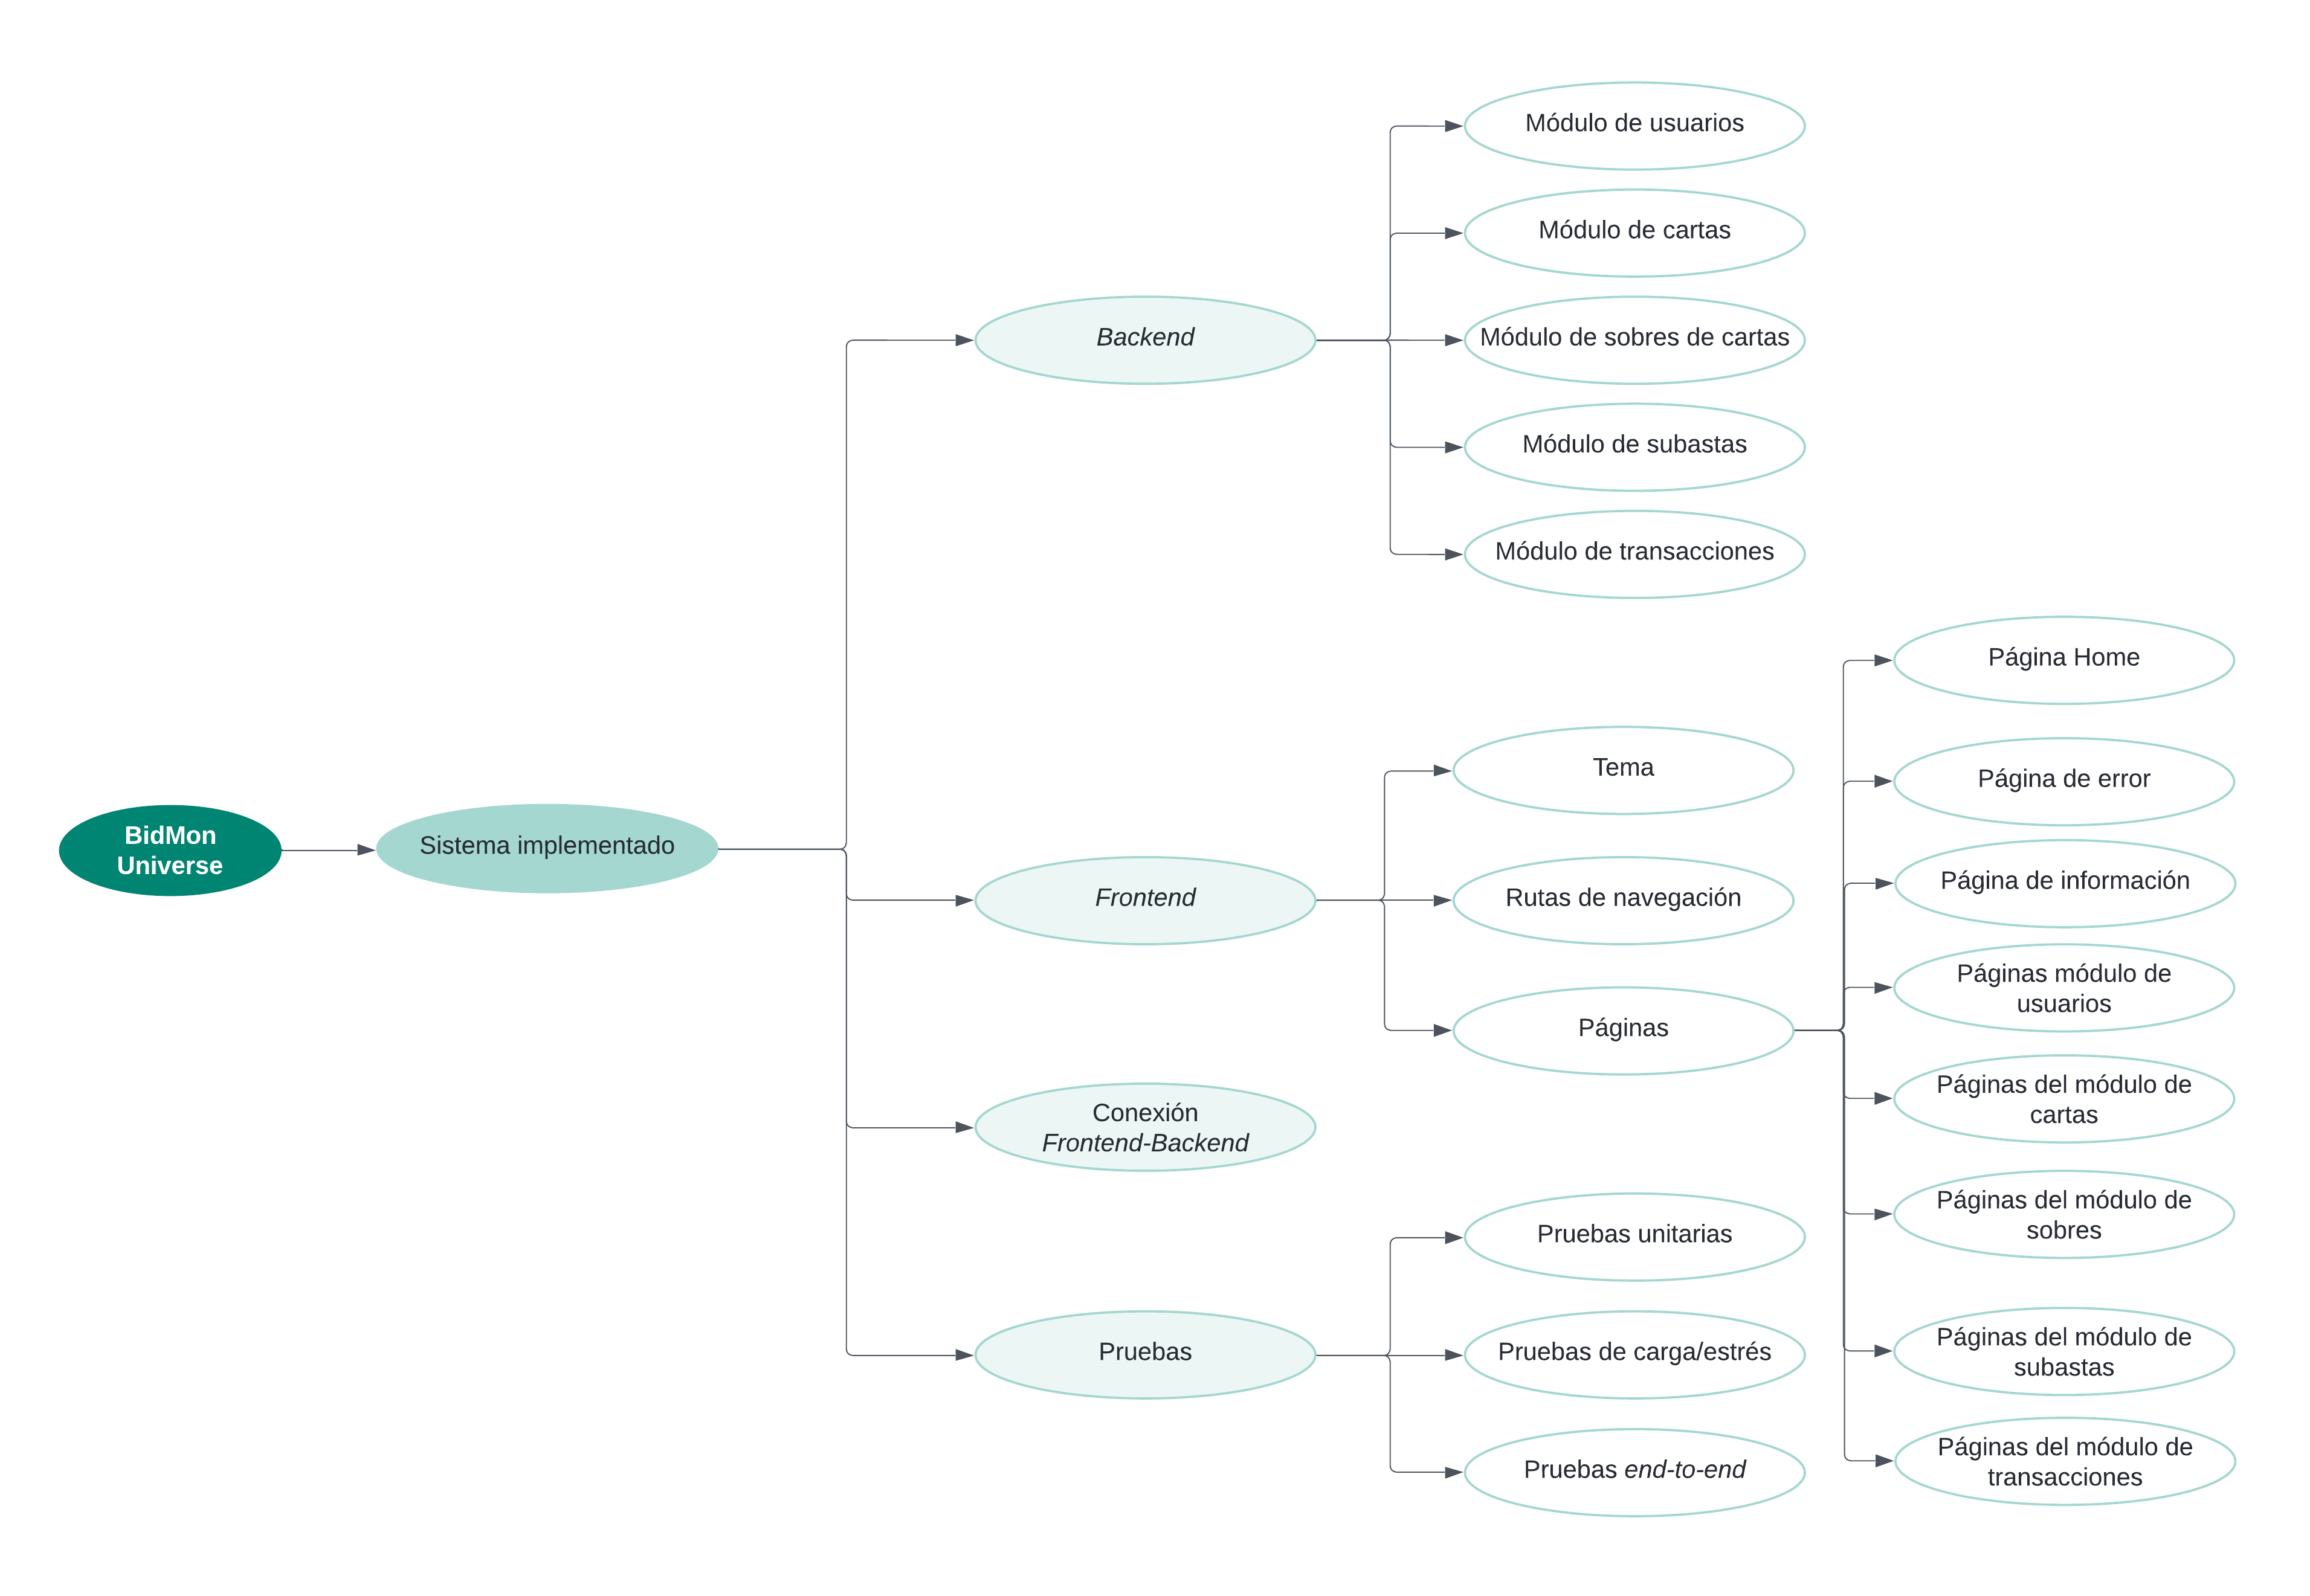
\includegraphics[width=0.9\linewidth]{figures/5-PBS/5_PBS-Implementacion.png}
    \caption{PBS. Implementación del sistema}
    \label{fig:5_PBS-Implementación-Sistema}
\end{figure}

\subsubsection{PBS. Pruebas del sistema}
En la fase de pruebas del sistema se obtienen como productos los resultados de la ejecución de dichas pruebas.
\begin{figure}[H]
    \hypertarget{fig:5_PBS-Pruebas-Sistema}{}
    \centering
    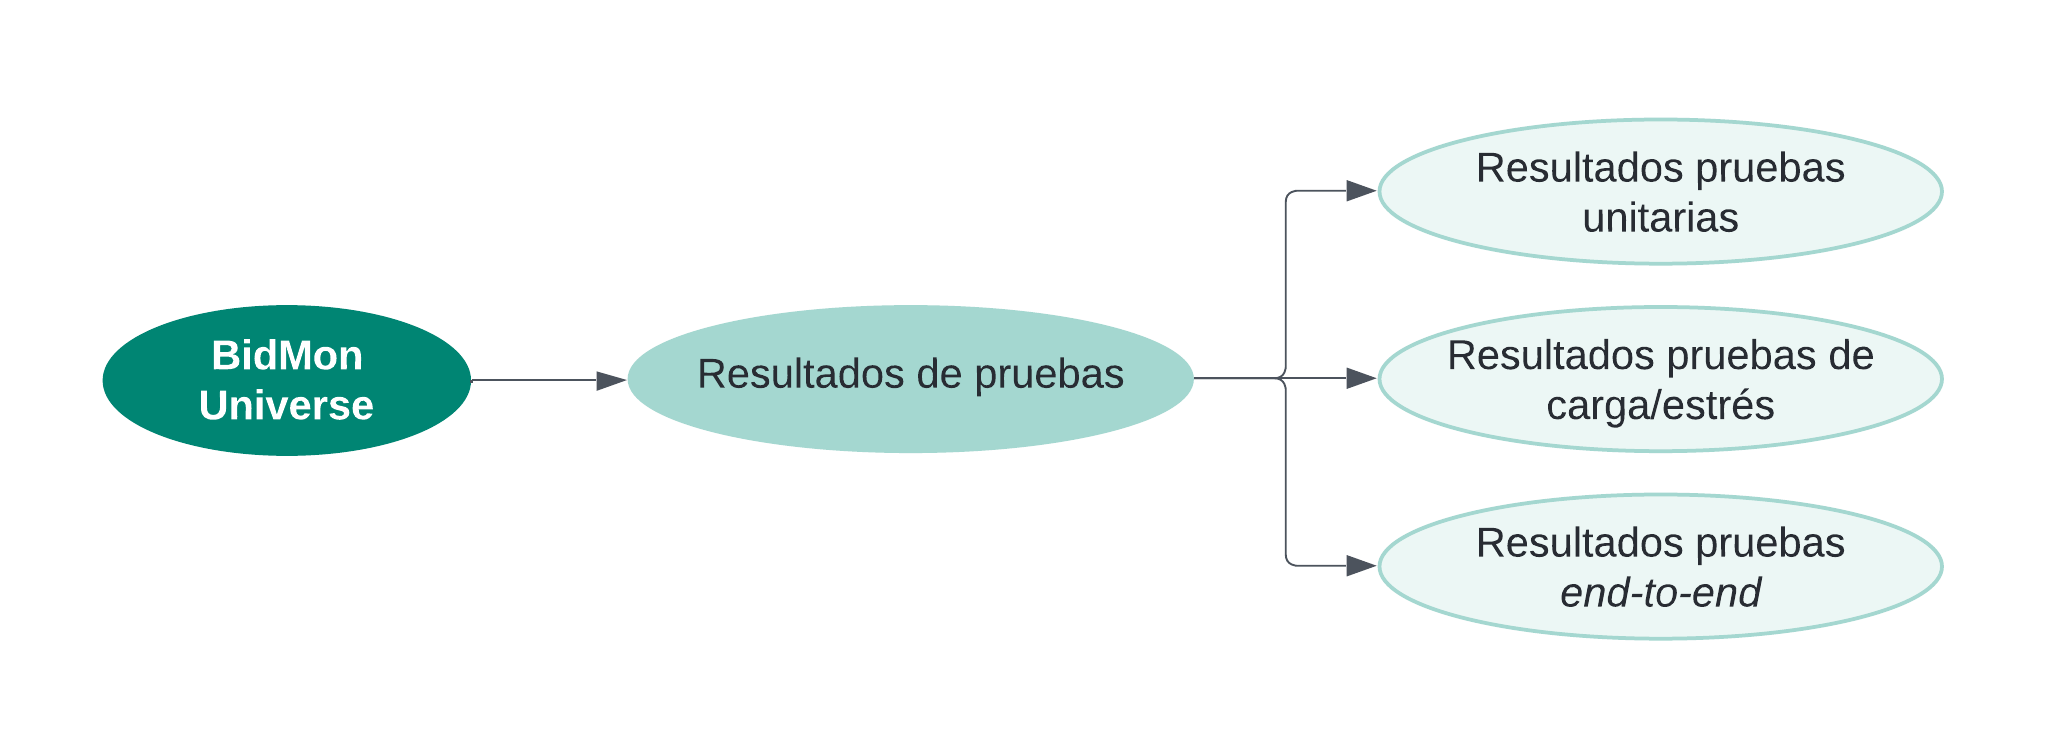
\includegraphics[width=0.7\linewidth]{figures/5-PBS/5_PBS-Pruebas.png}
    \caption{PBS. Pruebas del sistema}
    \label{fig:5_PBS-Pruebas-Sistema}
\end{figure}

\subsubsection{PBS. Despliegue del sistema}
En la fase de despliegue del sistema se obtiene como producto el sistema desplegado y en funcionamiento.
\begin{figure}[H]
    \hypertarget{fig:5_PBS-Despliegue-Sistema}{}
    \centering
    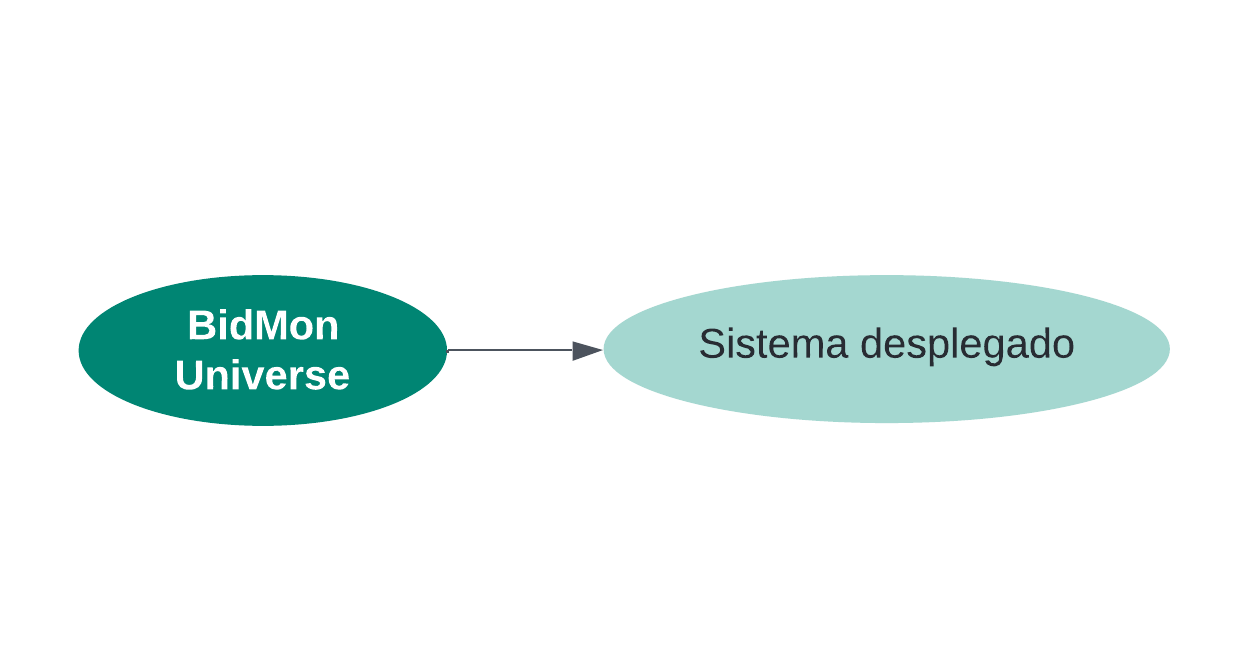
\includegraphics[width=0.7\linewidth]{figures/5-PBS/5_PBS-Despliegue.png}
    \caption{PBS. Despliegue del sistema}
    \label{fig:5_PBS-Despliegue-Sistema}
\end{figure}


\subsubsection{PBS. Documentación del sistema}
En la fase de documentación del sistema se obtienen como productos los documentos técnicos que describen el proyecto junto con los anexos.
\begin{figure}[H]
    \hypertarget{fig:5_PBS-Documentación-Sistema}{}
    \centering
    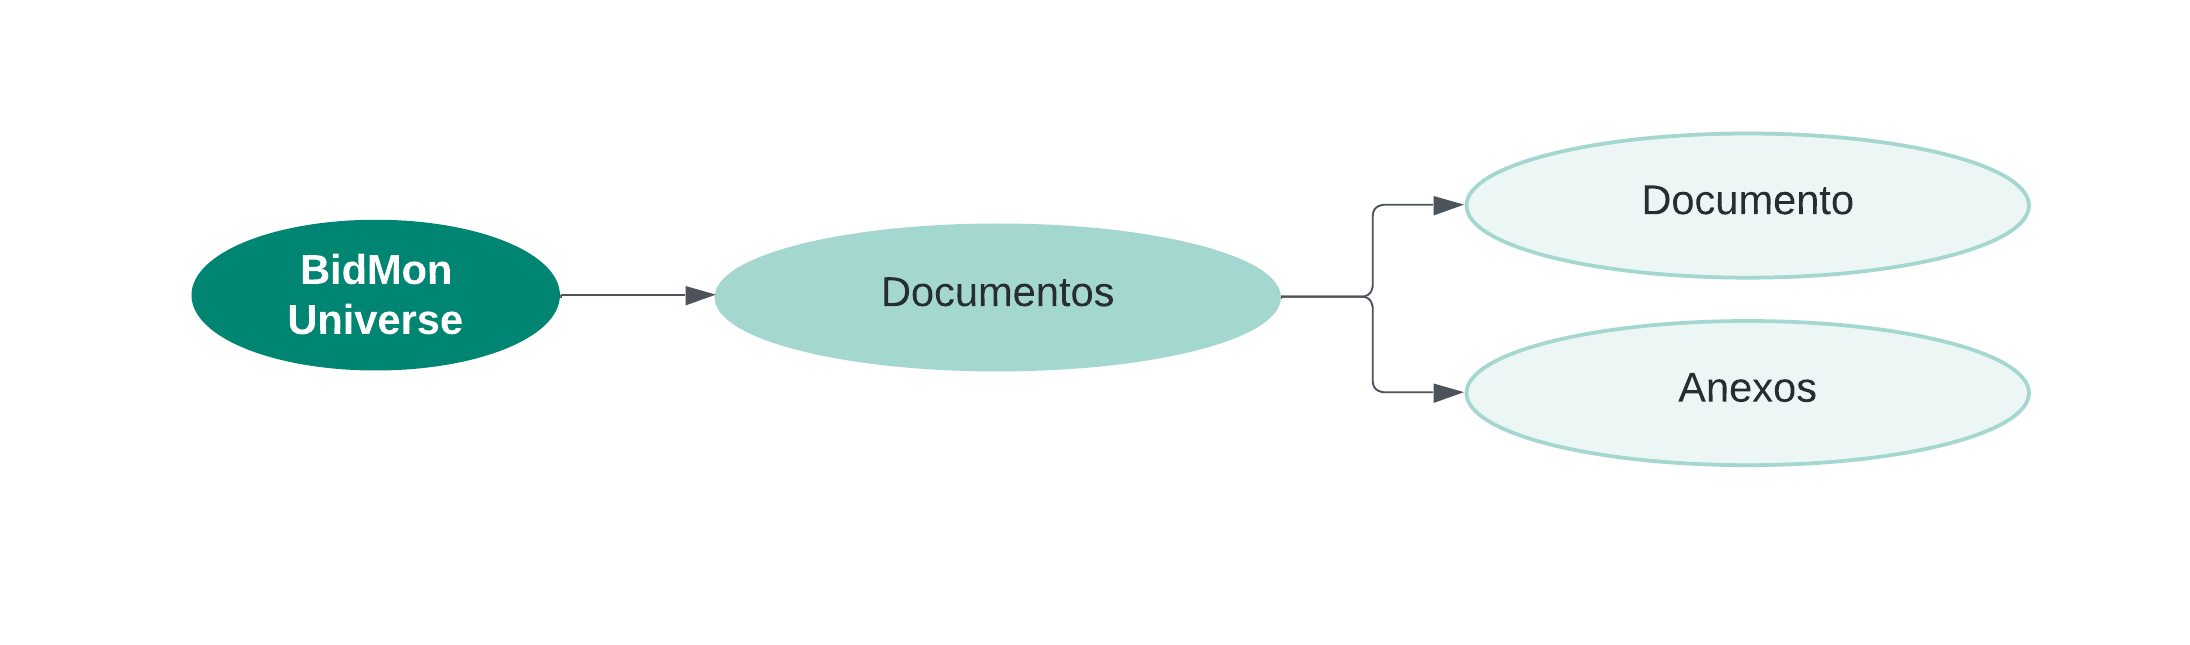
\includegraphics[width=0.7\linewidth]{figures/5-PBS/5_PBS-Documento.png}
    \caption{PBS. Documentación del sistema}
    \label{fig:5_PBS-Documentación-Sistema}
\end{figure}



\subsection{Planificación Inicial. WBS}
\subsubsection{WBS}
En esta sección se detalla la estructura de desglose del trabajo del proyecto también conocida como WBS, \textit{Work Breakdown Structure}. 
En ella se especifican las tareas necesarias para obtener los productos detallados en \coloredUnderline{\hyperlink{sec:5-PBS}{\ref*{sec:5-PBS} \nameref*{sec:5-PBS}}}.

Estas tareas se representan en forma de árbol jerárquico, donde cada rama representa una tarea y sus subramas las tareas que la componen.
El diagrama se ha dividido en las fases en las que se divide el proyecto para mejorar la legibilidad, facilitando la comprensión de las tareas y sub-tareas que se deben realizar en cada una de ellas.

\subsubsubsection{WBS. Visión general}
En la \coloredUnderline{\hyperlink{fig:5_WBS-Vision-General}{Figura \ref*{fig:5_WBS-Vision-General}: \nameref*{fig:5_WBS-Vision-General}}} se muestra la estructura de desglose del trabajo del proyecto de alto nivel, es decir, 
las tareas generales o fases que se deben realizar para cumplir con los objetivos del proyecto.
En las siguientes secciones, se entrará en detalle en cada una de las tareas.
\begin{figure}[H]
    \hypertarget{fig:5_WBS-Vision-General}{}
    \centering
    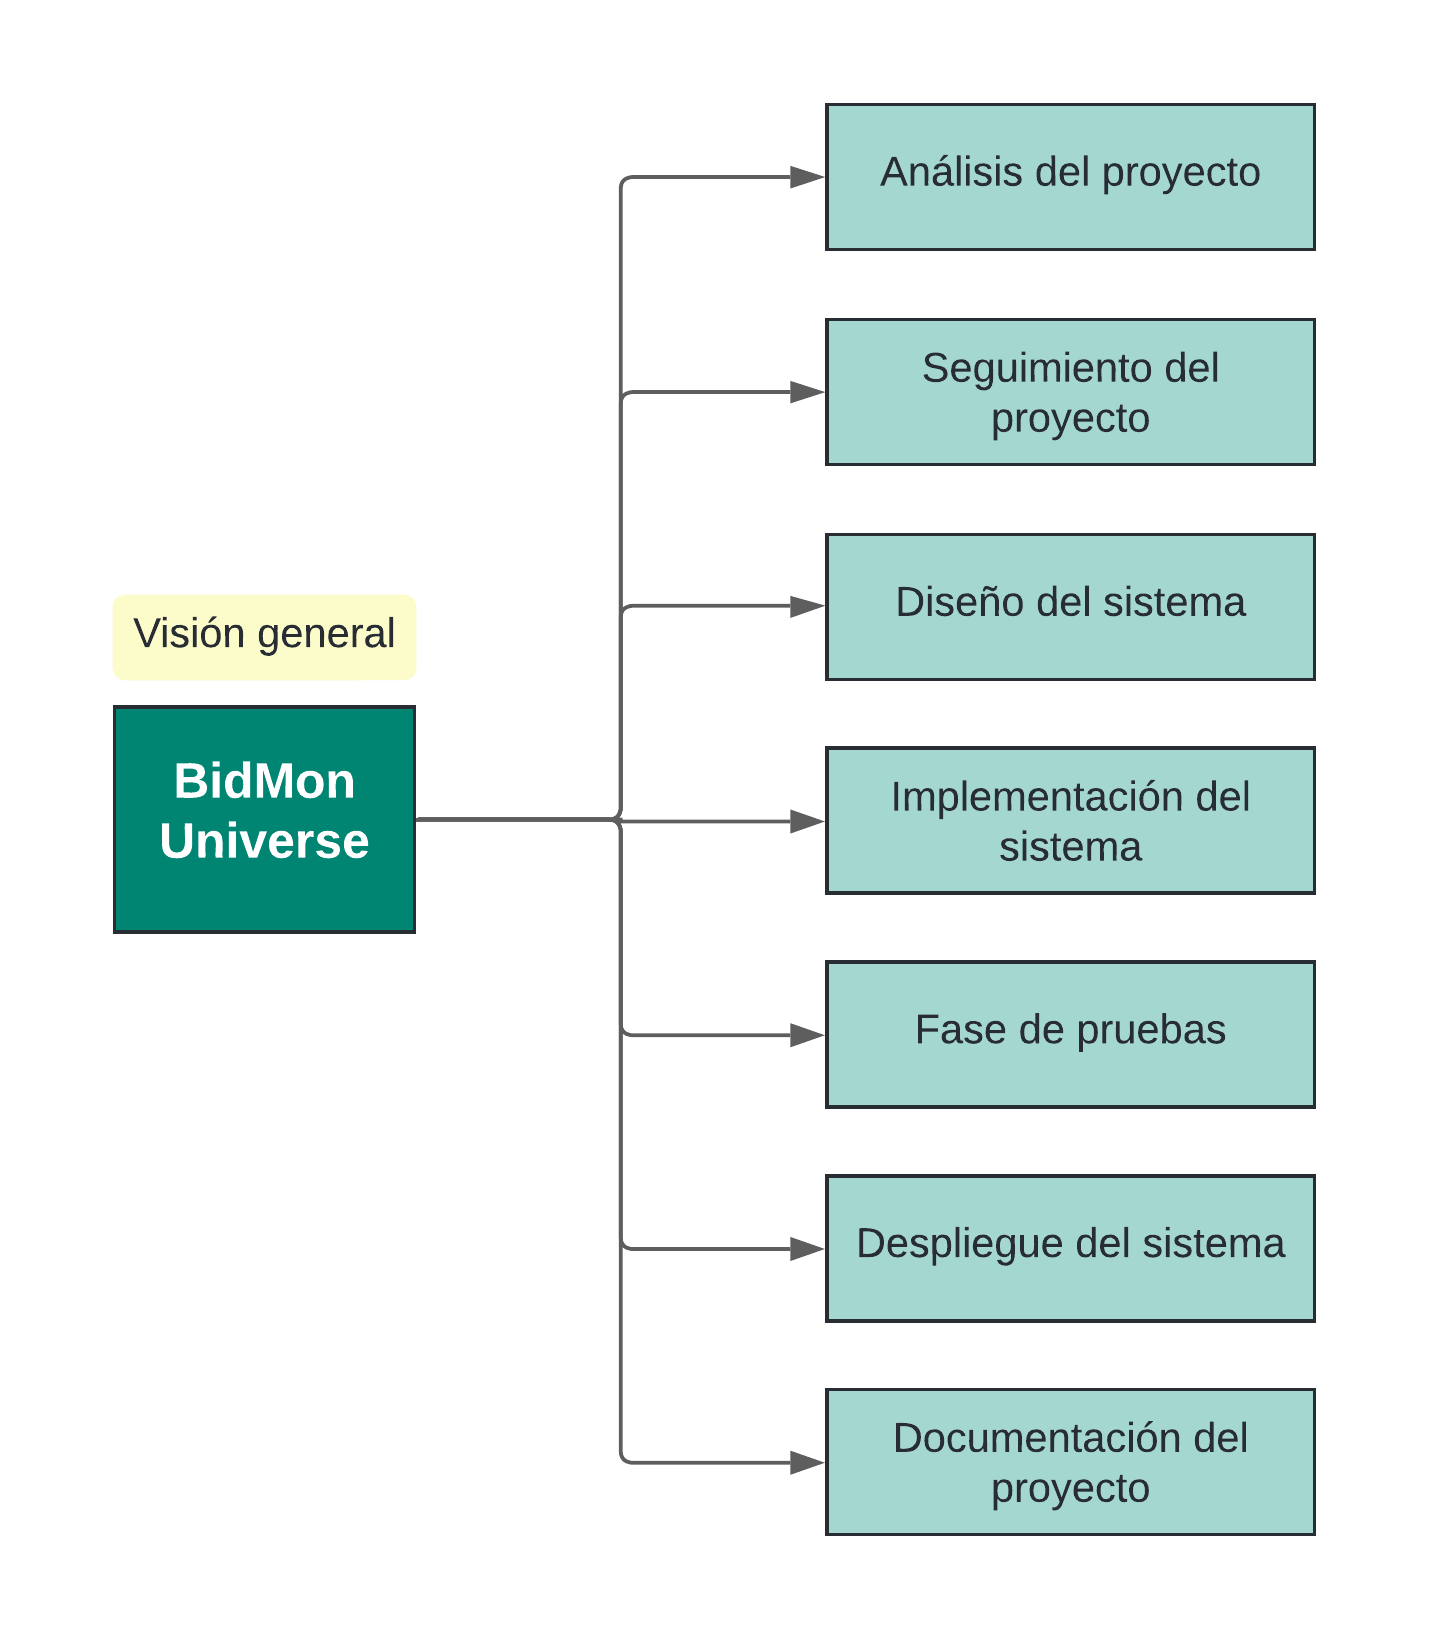
\includegraphics[width=0.5\linewidth]{figures/5-WBS/5_WBS-Vision-General.png}
    \caption{WBS. Visión general}
    \label{fig:5_WBS-Vision-General}
\end{figure}

\subsubsubsection{WBS. Análisis del proyecto}
En la \coloredUnderline{\hyperlink{fig:5_WBS-Analisis}{Figura \ref*{fig:5_WBS-Analisis}: \nameref*{fig:5_WBS-Analisis}}}, se detallan las tareas que se deben realizar en la fase de análisis del sistema para cumplir con los objetivos del proyecto.
\begin{figure}[H]
    \hypertarget{fig:5_WBS-Analisis}{}
    \centering
    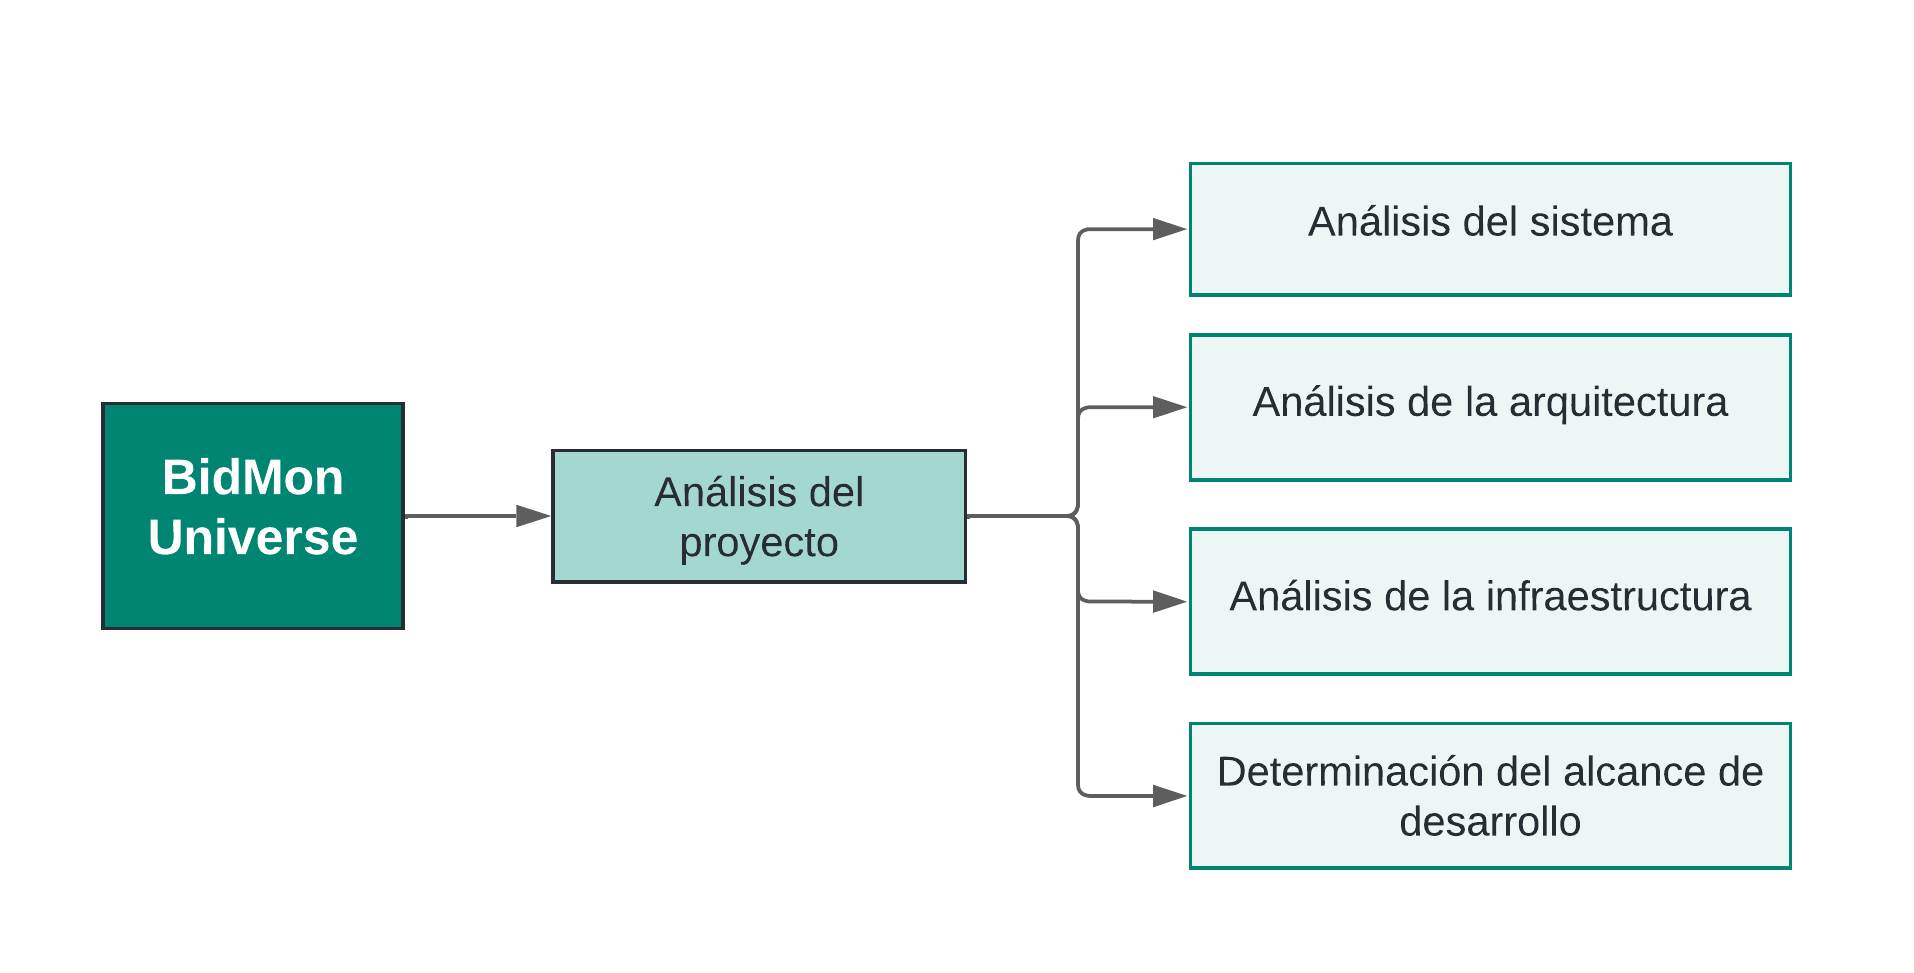
\includegraphics[width=0.7\linewidth]{figures/5-WBS/5_WBS-Analisis.png}
    \caption{WBS. Análisis del proyecto}
    \label{fig:5_WBS-Analisis}
\end{figure}

\subsubsubsection{WBS. Seguimiento del sistema}
En esta fase se realizan las tareas de seguimiento del proyecto, a través de distintas reuniones en las que se recopilará infomarción sobre el avance del proyecto. 
\begin{figure}[H]
    \hypertarget{fig:5_WBS-Seguimiento}{}
    \centering
    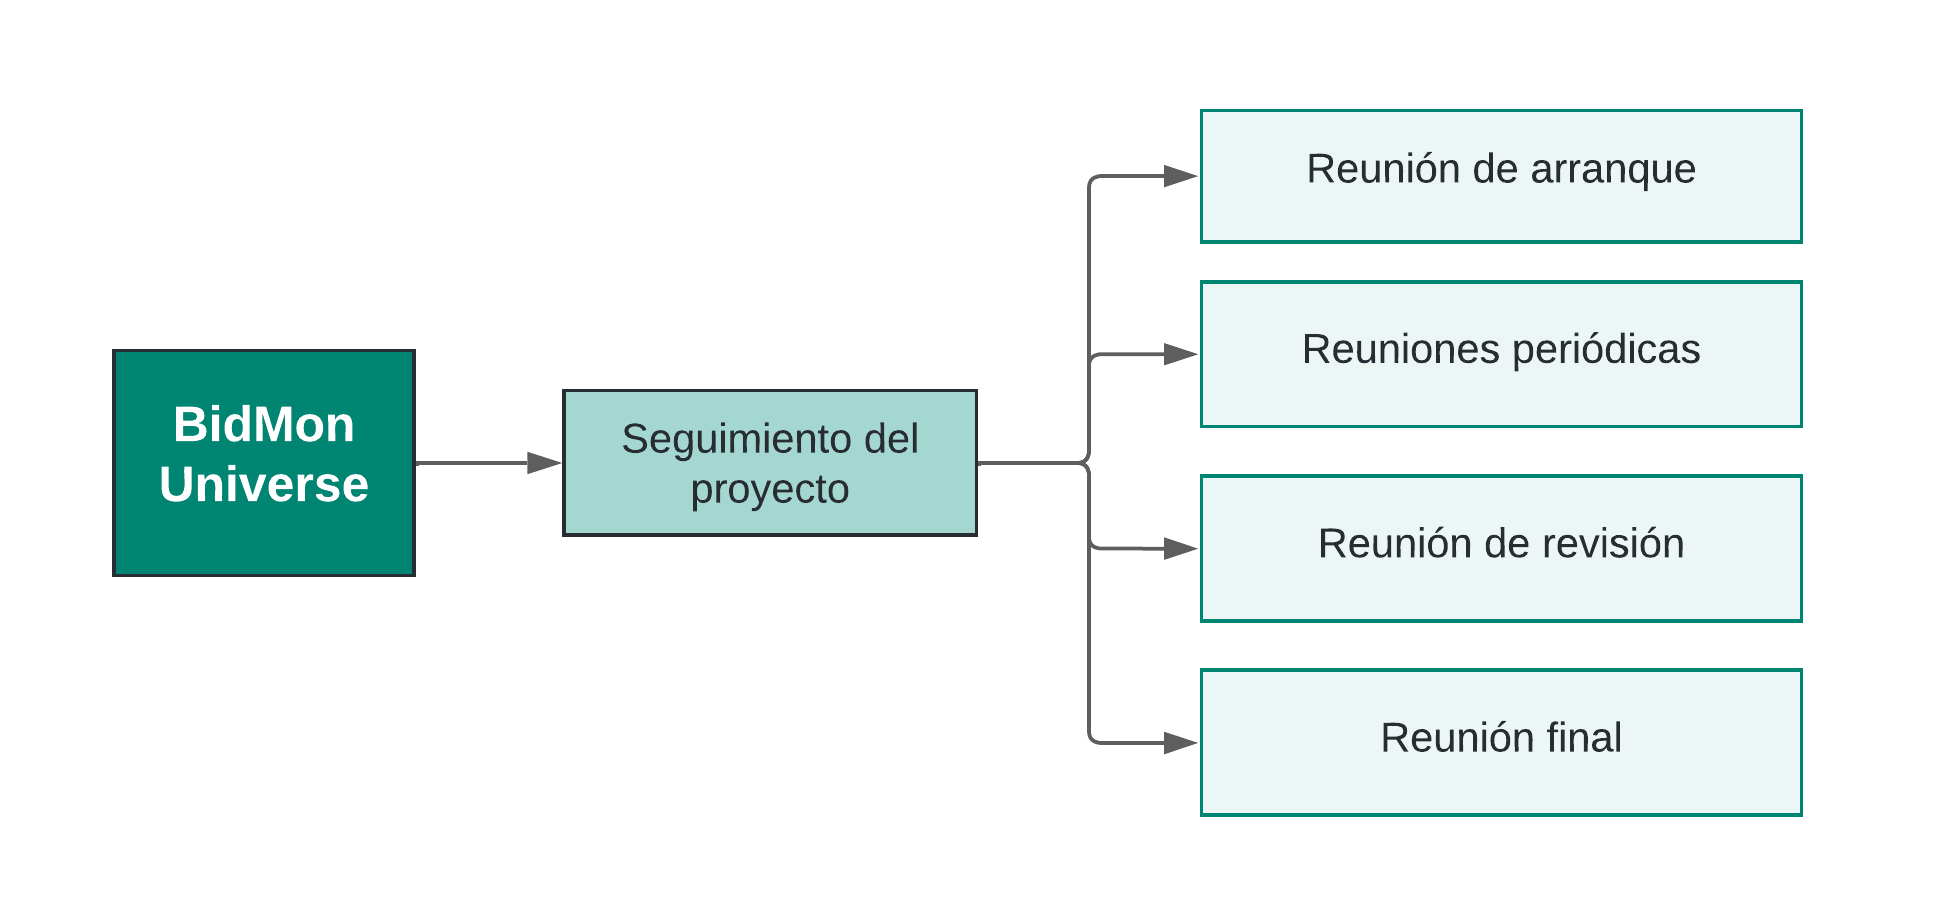
\includegraphics[width=0.7\linewidth]{figures/5-WBS/5_WBS-Seguimiento.png}
    \caption{WBS. Seguimiento del sistema}
    \label{fig:5_WBS-Seguimiento}
\end{figure}

\subsubsubsection{WBS. Diseño del sistema}
En la \coloredUnderline{\hyperlink{fig:5_WBS-Diseno}{Figura \ref*{fig:5_WBS-Diseno}: \nameref*{fig:5_WBS-Diseno}}}, se detallan las tareas que se deben realizar en la fase de diseño del sistema.
\begin{figure}[H]
    \hypertarget{fig:5_WBS-Diseno}{}
    \centering
    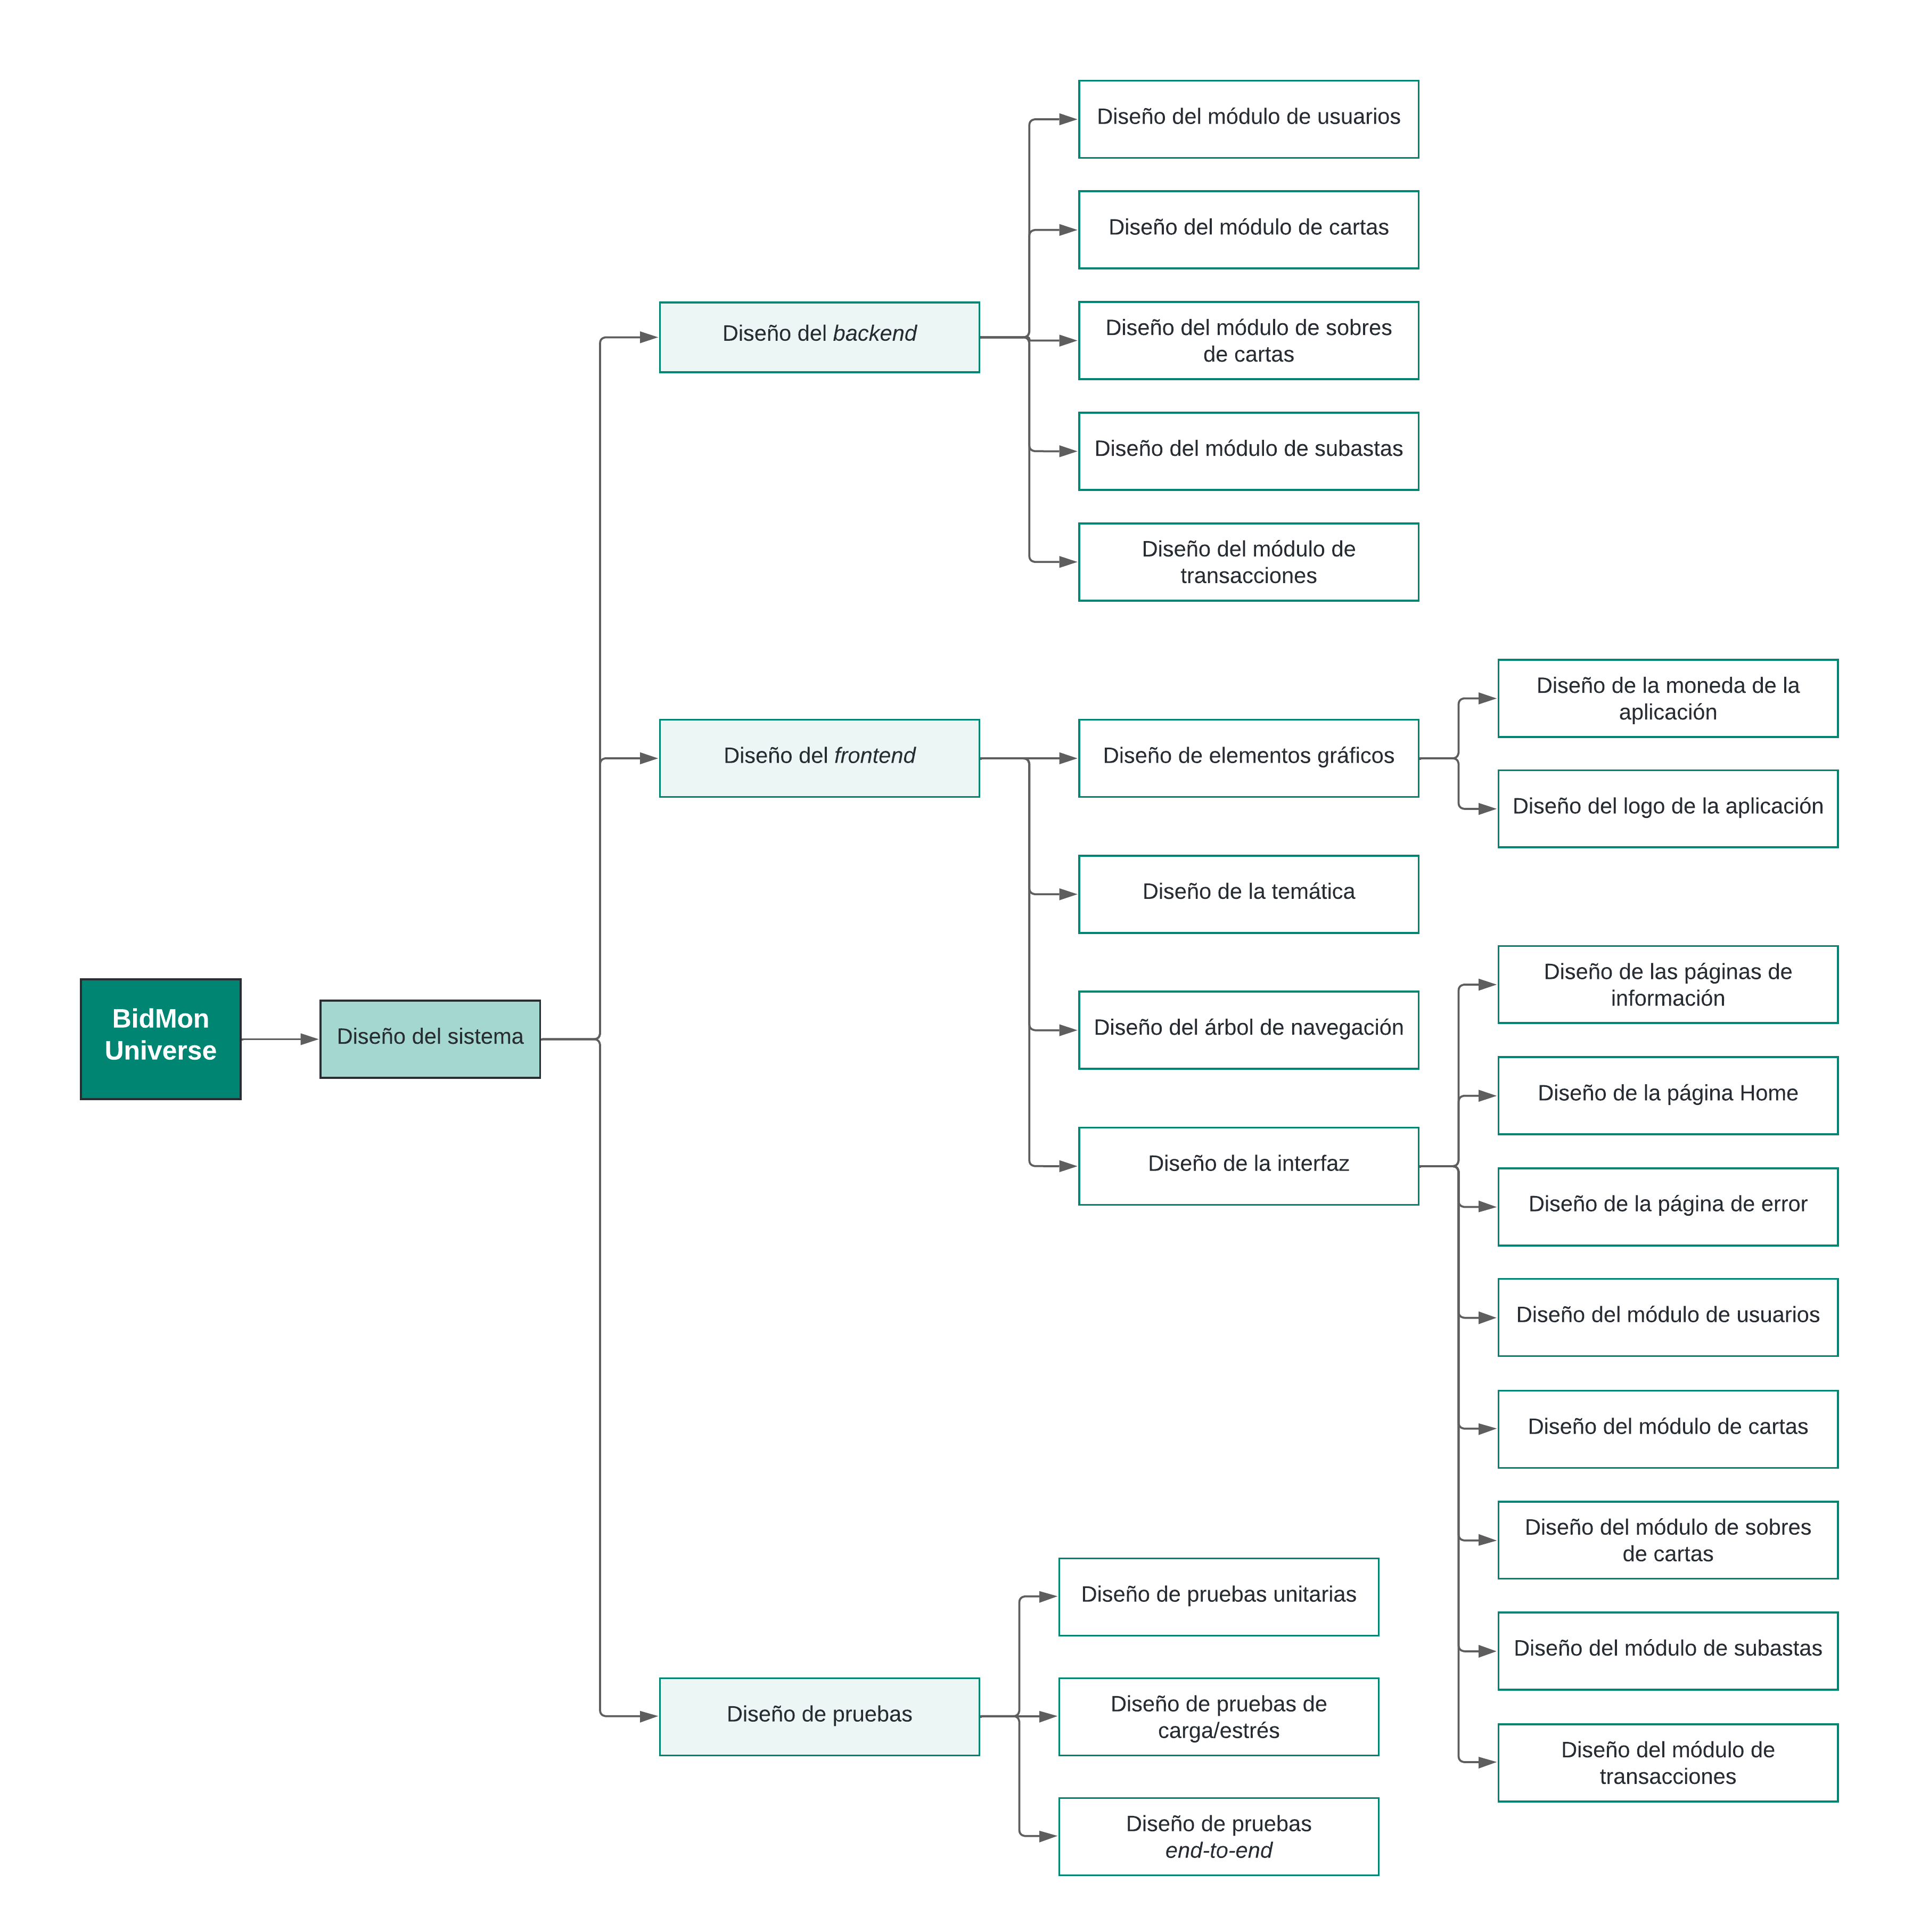
\includegraphics[width=0.9\linewidth]{figures/5-WBS/5_WBS-Diseno.png}
    \caption{WBS. Diseño del sistema}
    \label{fig:5_WBS-Diseno}
\end{figure}

\subsubsubsection{WBS. Implementación del sistema}
En la \coloredUnderline{\hyperlink{fig:5_WBS-Implementacion}{Figura \ref*{fig:5_WBS-Implementacion}: \nameref*{fig:5_WBS-Implementacion}}}, se detallan las tareas que se deben realizar en la fase de implementación del sistema.
\begin{figure}[H]
    \hypertarget{fig:5_WBS-Implementacion}{}
    \centering
    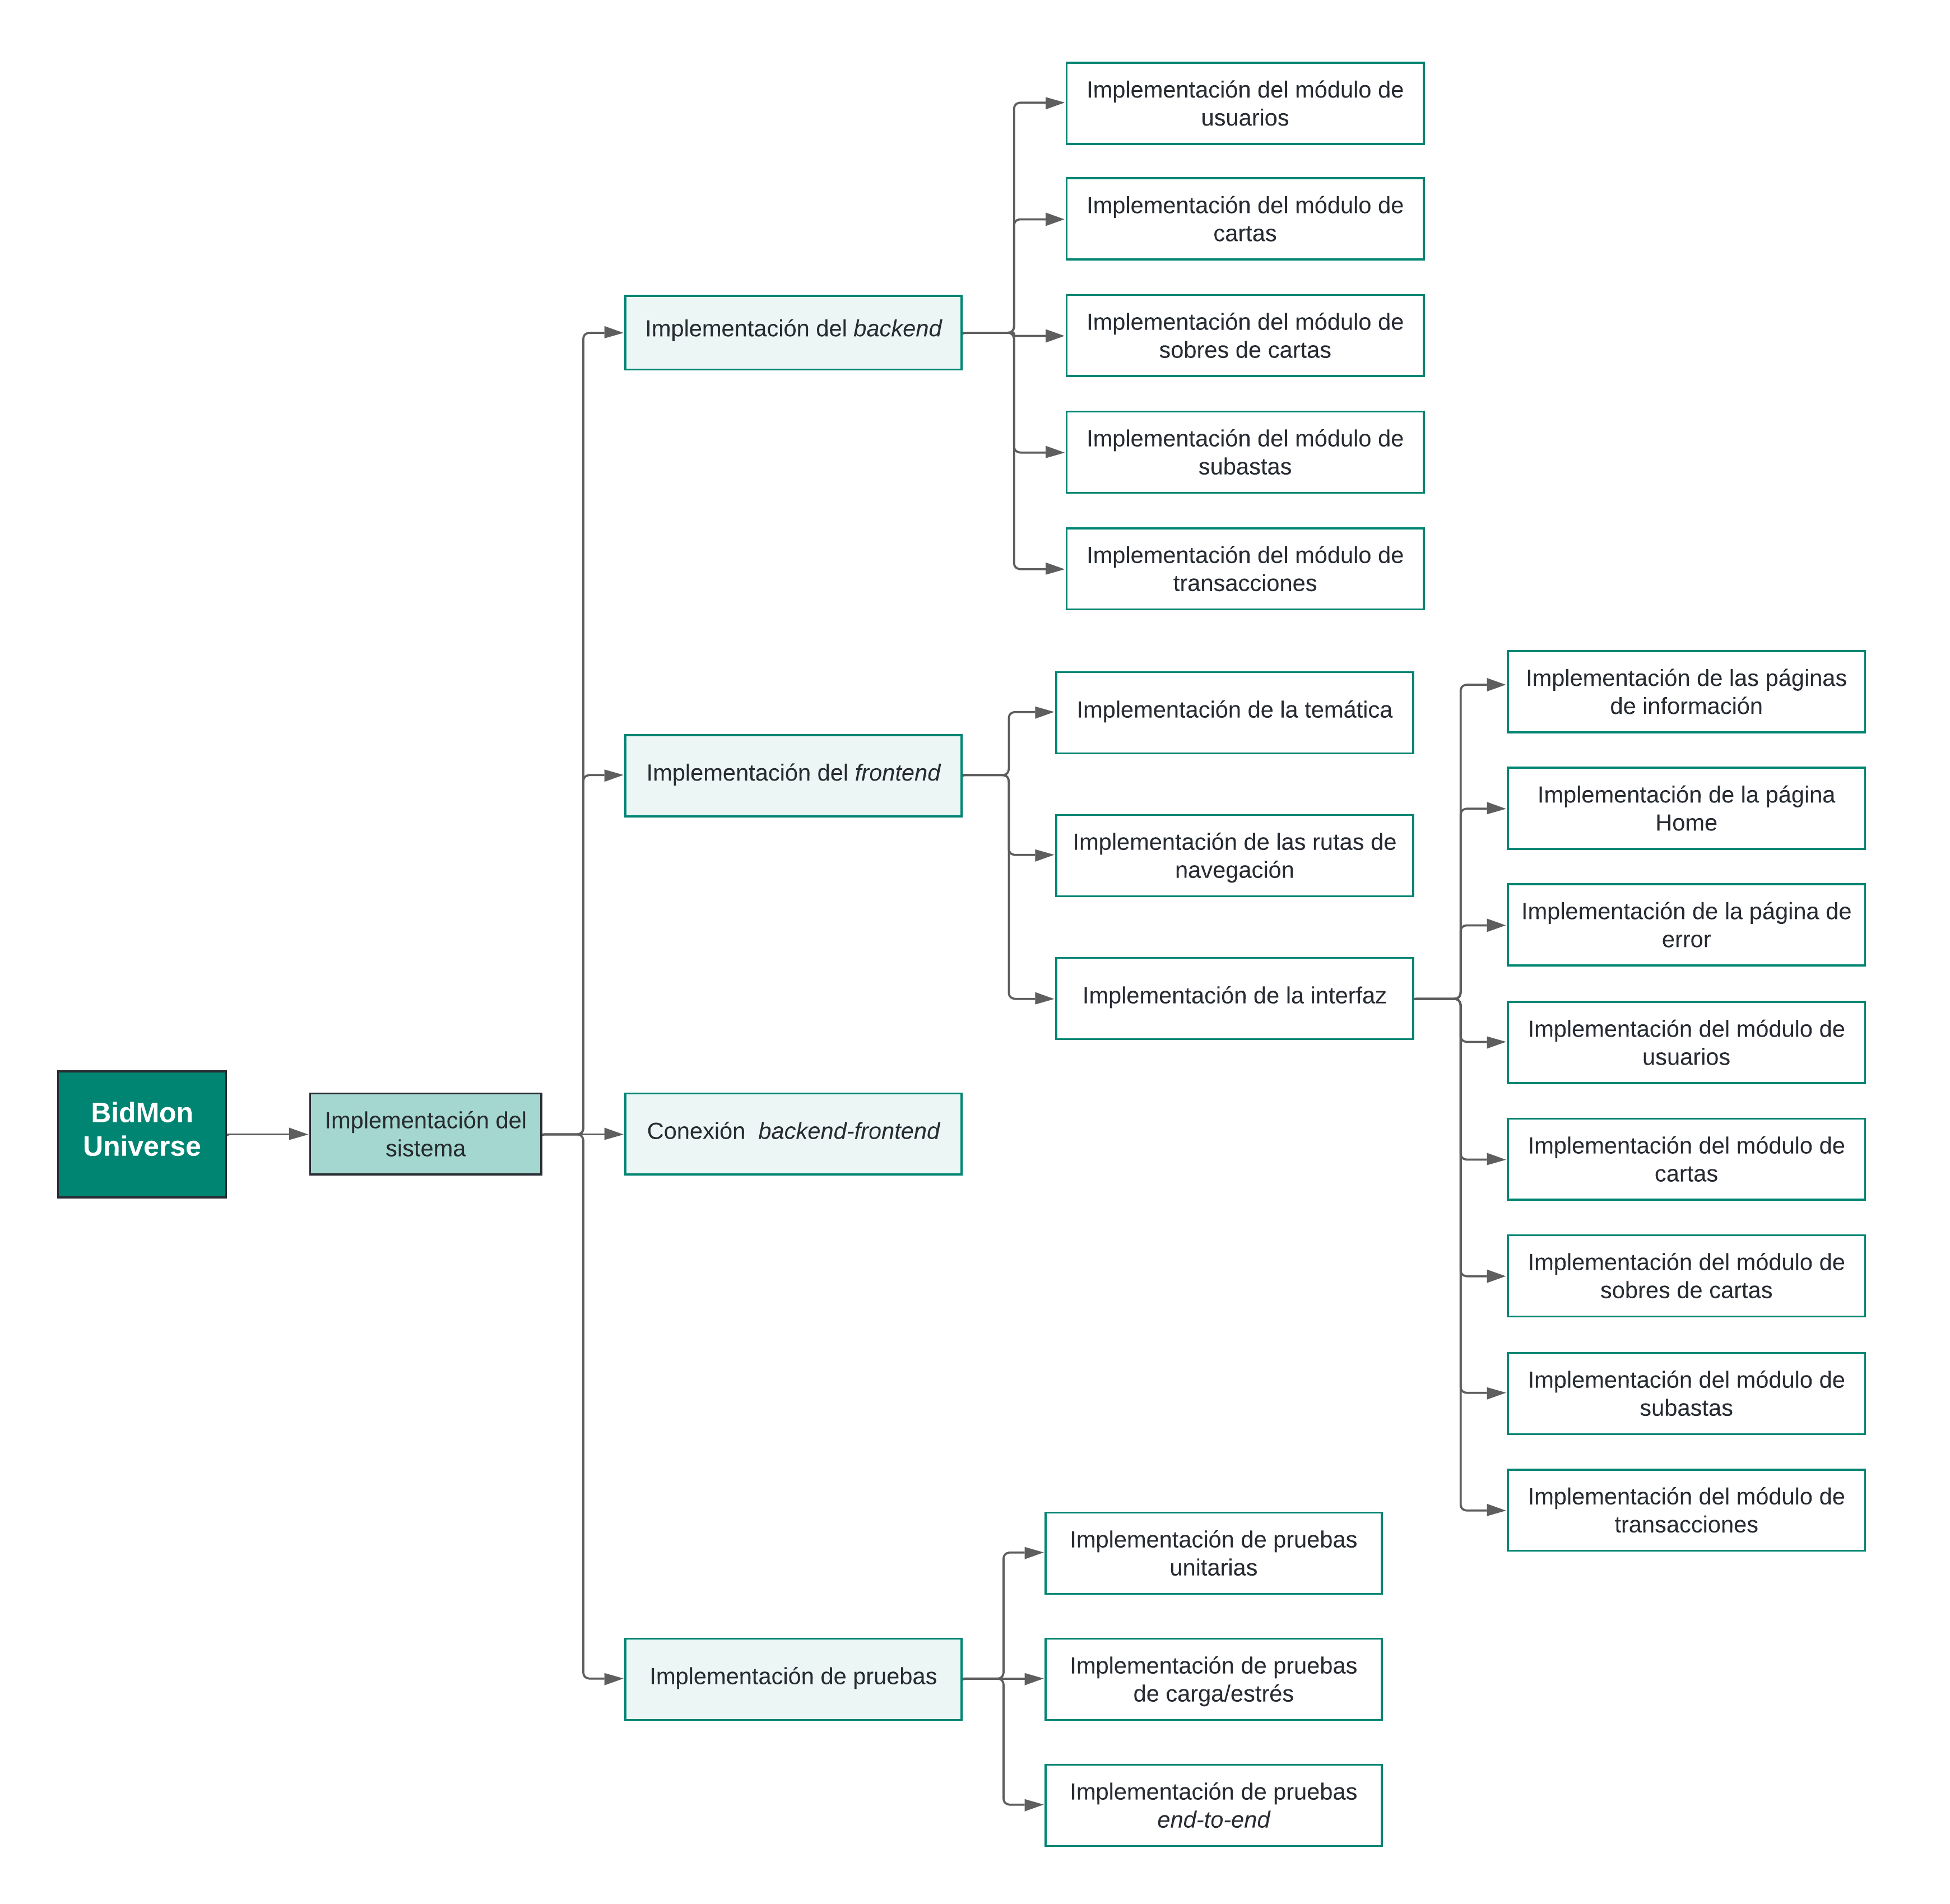
\includegraphics[width=0.9\linewidth]{figures/5-WBS/5_WBS-Implementacion.png}
    \caption{WBS. Implementación del sistema}
    \label{fig:5_WBS-Implementacion}
\end{figure}

\subsubsubsection{WBS. Fase de pruebas}
En la fase de pruebas del sistema se realizan las tareas necesarias para comprobar que el sistema cumple con los requisitos establecidos, recogiendo los informes especificados en \coloredUnderline{\hyperlink{fig:5_PBS-Pruebas}{Figura \ref*{fig:5_PBS-Pruebas}: \nameref*{fig:5_PBS-Pruebas}}}.
\begin{figure}[H]
    \hypertarget{fig:5_WBS-Pruebas}{}
    \centering
    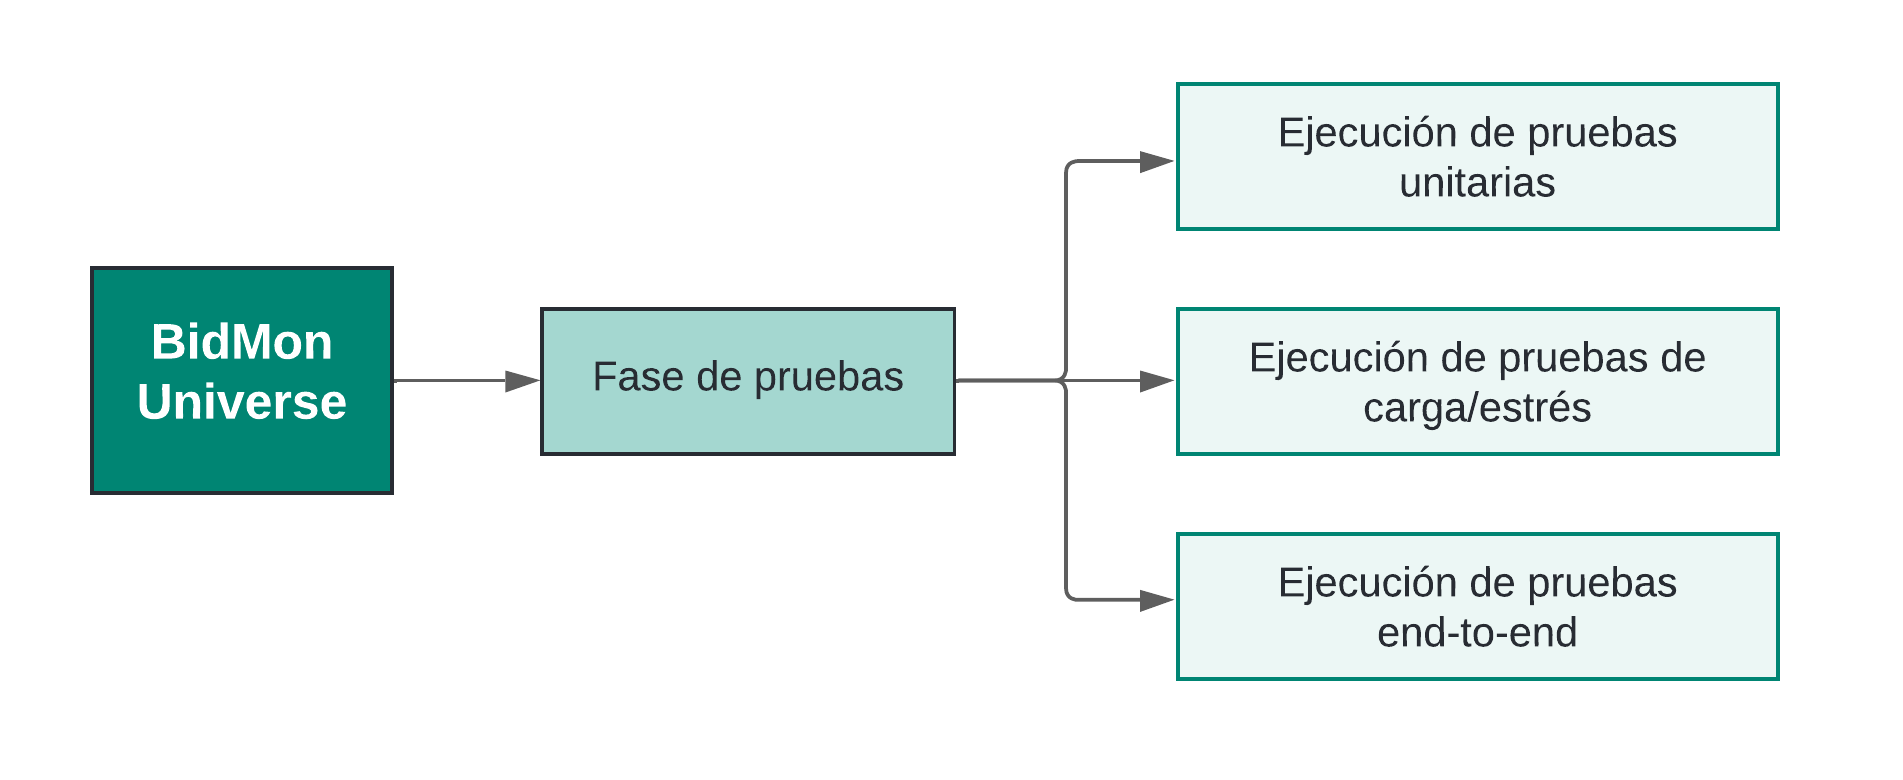
\includegraphics[width=0.9\linewidth]{figures/5-WBS/5_WBS-Pruebas.png}
    \caption{WBS. Fase de pruebas}
    \label{fig:5_WBS-Pruebas}
\end{figure}

\subsubsubsection{WBS. Despliegue del sistema}
En la fase de despliegue del sistema se realizan las tareas necesarias para poner en producción el sistema, como se detalla en la \coloredUnderline{\hyperlink{fig:5_WBS-Despliegue}{Figura \ref*{fig:5_WBS-Despliegue}: \nameref*{fig:5_WBS-Despliegue}}}.
\begin{figure}[H]
    \hypertarget{fig:5_WBS-Despliegue}{}
    \centering
    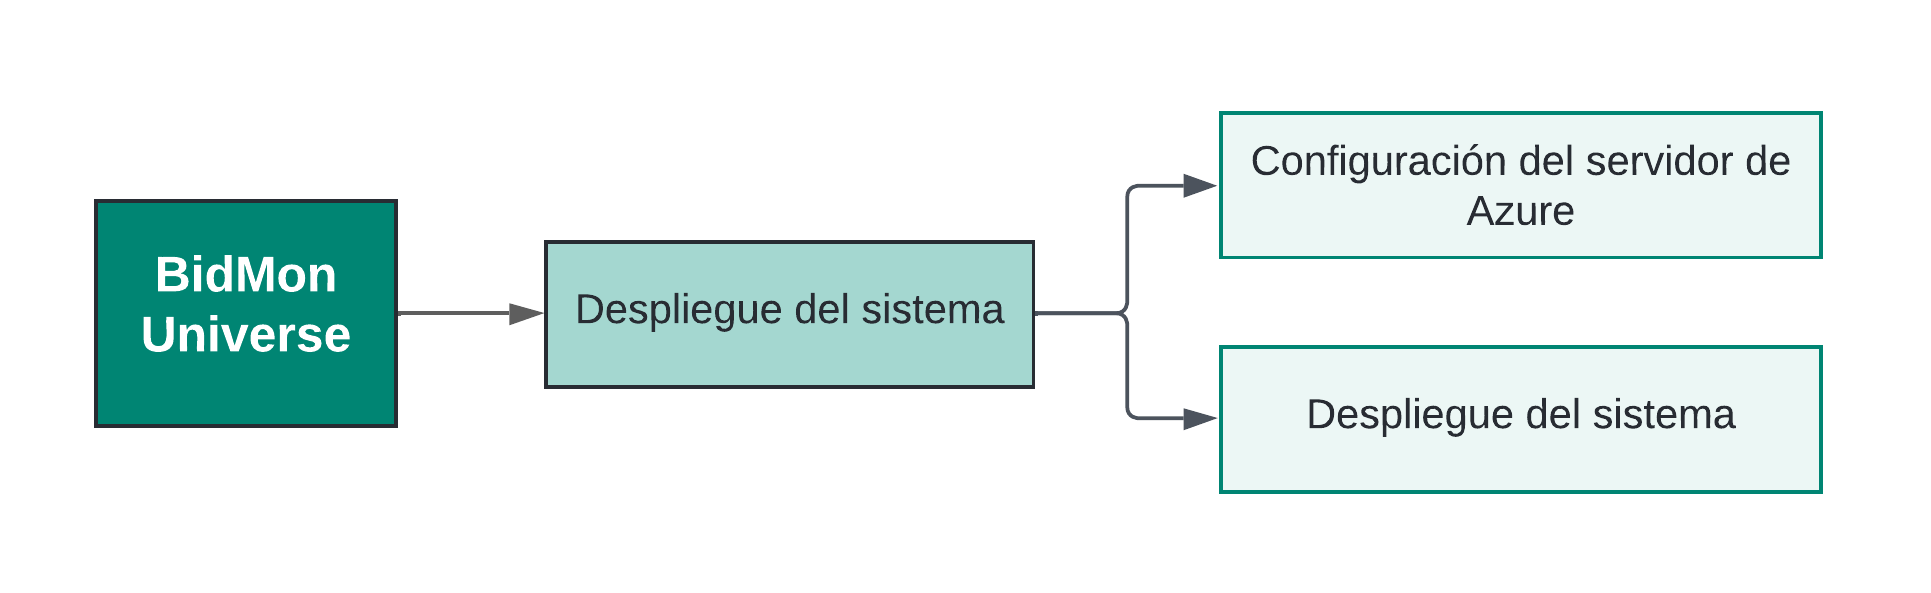
\includegraphics[width=0.9\linewidth]{figures/5-WBS/5_WBS-Despliegue2.png}
    \caption{WBS. Despliegue del sistema}
    \label{fig:5_WBS-Despliegue}
\end{figure}

\subsubsubsection{WBS. Documentación}
En la fase de documentación se realizan las tareas necesarias para la redacción de la memoria del proyecto, así como la preparación de la presentación del mismo.
\begin{figure}[H]
    \hypertarget{fig:5_WBS-Documentacion}{}
    \centering
    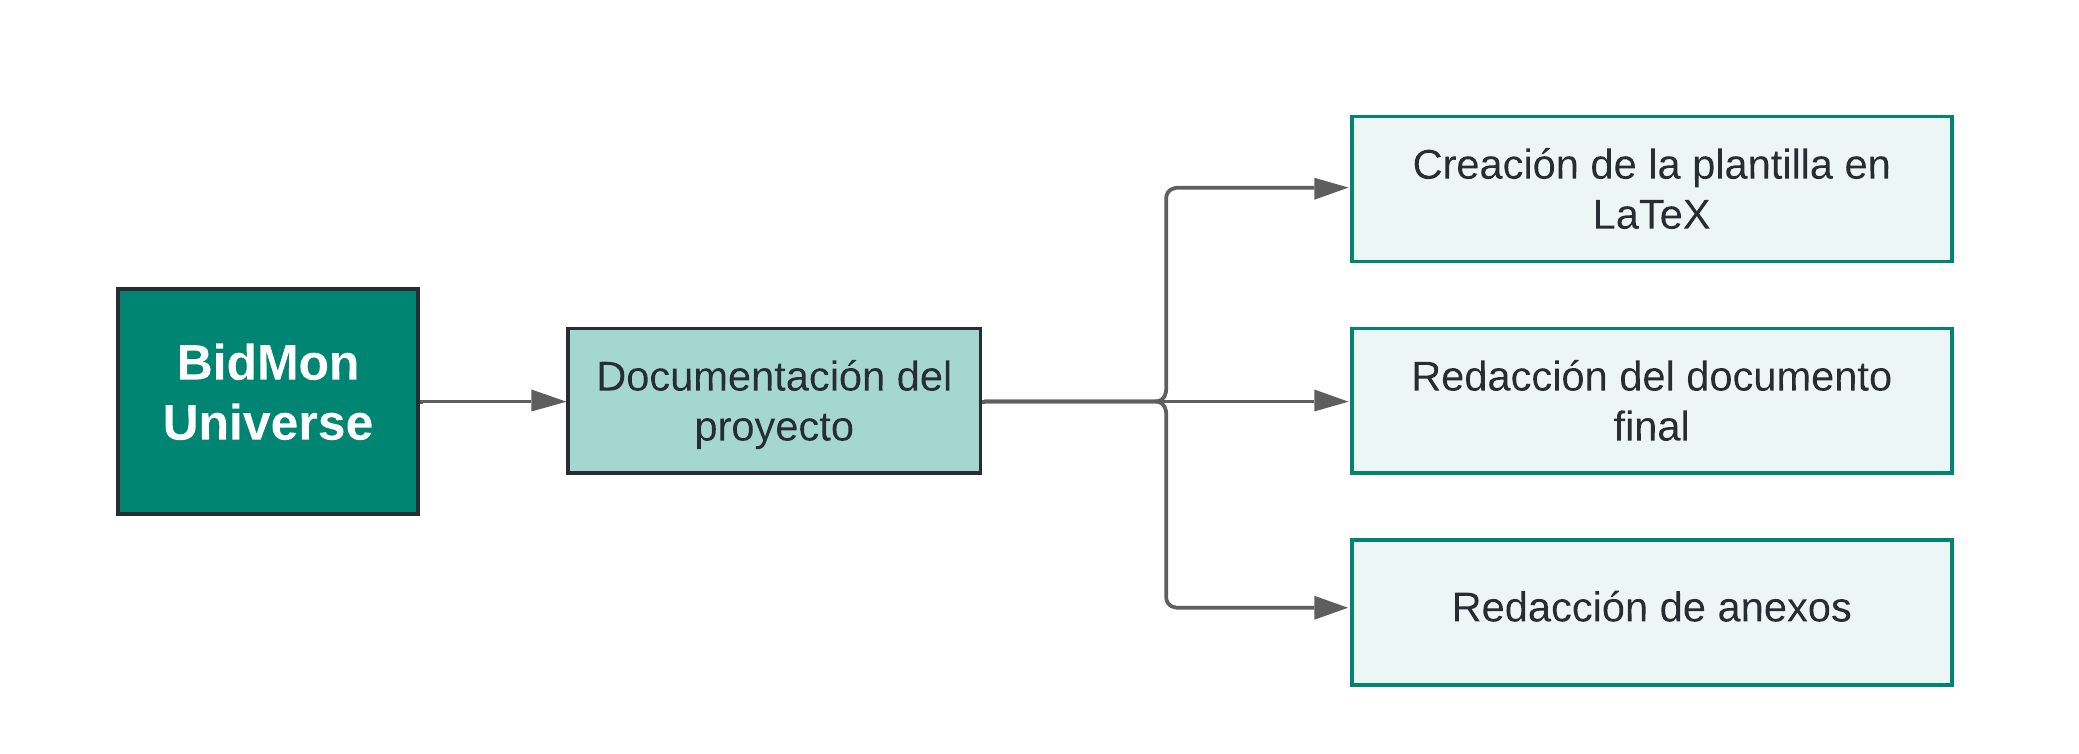
\includegraphics[width=0.9\linewidth]{figures/5-WBS/5_WBS-Documentacion.png}
    \caption{WBS. Documentación}
    \label{fig:5_WBS-Documentacion}
\end{figure}

\input{5-Planificacion-Gestion-TFG/5-Planificacion-inicial}


\subsection{Riesgos}
\subsubsection{Plan de Gestión de Riesgos} 

\subsubsection{Identificación de Riesgos}


\subsubsection{Registro de Riesgos} 

\begin{table}[htb]
    \centering
    \caption{Análisis de riesgo}
    \label{table:risk_analysis}
    \begin{tabular}{>{\columncolor{rowcolor}}l l l}
    \toprule
    \rowcolor{lightgreen}
    \textbf{Identificador} & \multicolumn{2}{l}{1} \\
    \midrule
    \textbf{Nombre} & \multicolumn{2}{l}{Problema de costos} \\
    \midrule
    \textbf{Descripción} & \multicolumn{2}{p{10cm}}{El costo de desarrollar y mantener un sitio web y un sistema de venta y distribución es alto, lo que puede afectar negativamente la rentabilidad de la empresa si no se generan suficientes ingresos para cubrir estos costos.} \\
    \midrule
    \textbf{Categoría} & \multicolumn{2}{l}{Riesgo de gestión} \\
    \midrule
    \textbf{Probabilidad} & \multicolumn{2}{l}{Media} \\
    \midrule
    \textbf{Impacto} & Presupuesto & Crítico \\
    \cmidrule(lr){2-3}
    & Planificación & Medio \\
    \cmidrule(lr){2-3}
    & Alcance & Alto \\
    \cmidrule(lr){2-3}
    & Calidad & Alto \\
    \cmidrule(lr){2-3}
    & Total & 0.45 \\
    \midrule
    \textbf{Respuesta} & \multicolumn{2}{p{10cm}}{Realizar un análisis financiero riguroso para determinar el costo total del proyecto, incluyendo los costos de desarrollo, mantenimiento, actualizaciones y otros gastos asociados. Establecer proyecciones financieras realistas para garantizar que la empresa pueda generar suficientes ingresos para cubrir estos costos y obtener una rentabilidad adecuada.} \\
    \midrule
    \textbf{Estrategia} & \multicolumn{2}{l}{Mitigar el riesgo} \\
    \bottomrule
    \end{tabular}
    \end{table}





\subsection{Presupuesto Inicial}

\subsubsection{Presupuesto de Costes}

\subsubsection{Presupuesto de Cliente} 


\newpage
\section{EJECUCIÓN DEL PROYECTO}

\subsection{Plan Seguimiento de Planificación}

\subsection{Bitácora de Incidencias del Proyecto}

\subsection{Riesgos}


\newpage
\section{CIERRE DEL PROYECTO}

\subsection{Planificación Final}

\subsection{Informe Final de Riesgos}

\subsection{Presupuesto Final de Costes}



\subsection{Informe de Lecciones Aprendidas}



\newpage
\chapter{ANÁLISIS DEL SISTEMA DE INFORMACIÓN}
\noindent\begin{tikzpicture}
% Definir el degradado
\shade[left color=darkgreen, right color=lightgreen] (0,0) rectangle (\textwidth-1pt,0.2);

\end{tikzpicture}
\newpage

\section{DEFINICIÓN DEL SISTEMA}
En este apartado se describirá brevemente el sistema a desarrollar indicando el alcance del mismo.
\subsection{Determinación del Alcance del Sistema}
BidMon Universe tiene como objetivo principal permitir al usuario coleccionar activos digitales, en este caso, cartas. Estas se pueden obtener mediante una compra directa a la aplicación o por medio de subastas. Para obtener más detalles sobre las funcionalidades de alto nivel, se puede consultar el apartado 
\coloredUnderline{\hyperlink{sec:2_identificacion_alcance_PSI}{2.1.2. Identificación del alcance del Plan de Sistemas de Información}}, y para una descripción más exhaustiva, ver el apartado \coloredUnderline{\hyperlink{sec:6_2-Requisitos}{6.2. Requisitos}}.
Es esencial establecer un sistema de trazabilidad robusto que registre cada transacción de compra y venta dentro de la aplicación de manera clara e inequívoca, asegurando la integridad y la transparencia de todas las operaciones.
En esta versión del sistema, la carga inicial de datos se llevará a cabo una única vez. Los administradores del sistema no podrán añadir nuevas cartas a través de la interfaz de usuario, cualquier adición de nuevas cartas se realizará directamente en la base de datos. Además, la plataforma no incluirá una opción que permita a los usuarios exportar la colección de cartas que posean.
La aplicación no incluye un sistema de mensajería interna ni permite la formación de relaciones sociales directas entre los usuarios, tales como "amistades" o conexiones similares. La plataforma se centra exclusivamente en las transacciones y la colección de cartas.



\subsection{Identificación de Actores del Sistema} 
El sistema está diseñado para soportar tres categorías principales de usuarios, cada uno con niveles de acceso y funcionalidades específicas adecuadas a su rol dentro de la plataforma:
\begin{enumerate}
    \item \textbf{Usuarios Invitados}
    \begin{itemize}
        \item Tienen acceso limitado exclusivamente a la página de bienvenida y a otras páginas informativas de acceso público dentro de la plataforma.
        \item El objetivo es proporcionar a los usuarios no registrados información general sobre la plataforma y sus características sin comprometer la seguridad o la privacidad de las transacciones y actividades de los usuarios registrados.
    \end{itemize}
    
    \item \textbf{Usuarios Autenticados}
    \begin{itemize}
        \item Tienen acceso a todas las funcionalidades operativas de la plataforma, incluyendo la colección de cartas, compra y subasta de estas.
    \end{itemize}
    
    \item \textbf{Usuarios Administradores}
    \begin{itemize}
        \item El acceso estaría limitado a la consulta de subastas activas, capacidad de intervenir en una subasta que considere fraudulenta y acceso al histórico de transacciones.
    \end{itemize}
\end{enumerate}


\newpage
\section{ESTABLECIMIENTO DE REQUISITOS}
\subsection{Obtención de los Requisitos del Sistema} \label{sec:6_2-requisitos}

\subsubsection{Requisitos funcionales}

\newlist{RFGestionUsuarios}{enumerate}{5}
\setlist[RFGestionUsuarios,1]{label=\textbf{RGU-\arabic*.}, leftmargin=*, align=left, font=\fontsize{10pt}{11pt}\selectfont}
\setlist[RFGestionUsuarios,2]{label*=\textbf{\arabic*.},font=\fontsize{10pt}{11pt}\selectfont}
\setlist[RFGestionUsuarios,3]{label*=\textbf{\arabic*.},font=\fontsize{9pt}{11pt}\selectfont}
\setlist[RFGestionUsuarios,4]{label*=\textbf{\arabic*.},font=\fontsize{8pt}{11pt}\selectfont}
\setlist[RFGestionUsuarios,5]{label*=\textbf{\arabic*.},font=\fontsize{8pt}{11pt}\selectfont}


\subsubsubsection{Registro e inicio de sesión}
\begin{RFGestionUsuarios}
	\item Un usuario deberá poder registrarse en el sistema.\label{req_registro}
	\begin{RFGestionUsuarios}
		\item El usuario deberá proporcionar el nombre de usuario que desea utilizar.
			\begin{RFGestionUsuarios}
				\item El sistema verificará que el nombre de usuario está disponible.
				\item El sistema verificará que el nombre de usuario cumpla con las restricciones de formato especificadas en \coloredUnderline{\hyperlink{confParam:gu-nombreUsuario}{GU\_NOMBRE\_USUARIO}}.
			\end{RFGestionUsuarios} 
		\item El usuario deberá proporcionar una contraseña.
			\begin{RFGestionUsuarios}
				\item El sistema asegurará que la contraseña cumpla con las políticas de seguridad especificadas en \coloredUnderline{\hyperlink{confParam:gu-contrasena}{GU\_CONTRASEÑA}}.
			\end{RFGestionUsuarios}
		\item El usuario deberá de confirmar la contraseña
			\begin{RFGestionUsuarios}
				\item El sistema verificará que la contraseña y su confirmación coincidan.
			\end{RFGestionUsuarios}
		\item El usuario deberá de especificar la fecha de nacimiento.
			\begin{RFGestionUsuarios}
               	\item El sistema verificará que la fecha de nacimiento está en el formato \coloredUnderline{\hyperlink{confParam:gu-fechaNacimiento}{GU\_FECHA\_NACIMIENTO}}.
				\item El sistema verificará que el usuario cumple con \coloredUnderline{\hyperlink{confParam:gu-minEdad}{GU\_MIN\_EDAD}}.
			\end{RFGestionUsuarios}
		\item Si alguno de los datos introducidos no cumple con las restricciones especificadas, el sistema mostrará un mensaje de error.
		\item Una vez finalizado el registro, el sistema registrará los datos en la base de datos:
			\begin{RFGestionUsuarios}
				\item Nombre de usuario
				\item Nombre de usuario en minúsculas
				\item Contraseña cifrada
				\item Fecha de nacimiento
				\item Fecha de creación
				\item \coloredUnderline{\hyperlink{confParam:gu-rolDefecto}{GU\_ROL\_DEFECTO}}
				\item \coloredUnderline{\hyperlink{confParam:gu-imgPerfilDefecto}{GU\_IMG\_PERFIL\_DEFECTO}}
				\item \coloredUnderline{\hyperlink{confParam:gu-saldoDefecto}{GU\_SALDO\_DEFECTO}}
			\end{RFGestionUsuarios}
		\item El sistema notificará al usuario que el registro ha sido completado con éxito.
		\item El usuario será redirigido a la pantalla de inicio de sesión.
	\end{RFGestionUsuarios}

	\item Un usuario podrá iniciar sesión en el sistema.\label{req_inicio_sesion}
    \begin{RFGestionUsuarios}%RF2.1
      \item Un usuario deberá proporcionar las siguientes credenciales para iniciar sesión:
		\begin{RFGestionUsuarios}
		  \item Nombre de usuario.
		  \item Contraseña.
		\end{RFGestionUsuarios}
	  \item El sistema validará las credenciales introducidas.
		\begin{RFGestionUsuarios}
			\item El sistema comprobará que el nombre de usuario existe en la base de datos.
			\item El sistema comprobará que la contraseña se corresponde con la registrada para dicho nombre de usuario.
		\end{RFGestionUsuarios}

      \item Si las credenciales son correctas:
		\begin{RFGestionUsuarios}
			\item El sistema redirigirá al usuario a la pantalla principal.
			\item Se generará un token de sesión con las restricciones \coloredUnderline{\hyperlink{confParam:gu-tokenSesion}{GU\_TOKEN\_SESION}}.
			\item El sistema establecerá una conexión Socket con el cliente para notificarle de eventos en tiempo real.
		\end{RFGestionUsuarios}
	  \item Si las credenciales son incorrectas:
		\begin{RFGestionUsuarios}
			\item El sistema mostrará un mensaje de error.
			\item El usuario podrá intentar iniciar sesión de nuevo.
		\end{RFGestionUsuarios}
    \end{RFGestionUsuarios}

	\item Un usuario autenticado podrá cerrar sesión en el sistema.\label{req_cerrar_sesion}
	\begin{RFGestionUsuarios}
		\item El sistema invalidará el token de sesión.
		\item El sistema cerrará la conexión Socket con el cliente.
		\item El sistema redirigirá al usuario a la pantalla de inicio.
	\end{RFGestionUsuarios}

\end{RFGestionUsuarios}


\newlist{RFColeccionCartas}{enumerate}{5}
\setlist[RFColeccionCartas,1]{label=\textbf{RCC-\arabic*.}, leftmargin=*, align=left, font=\fontsize{10pt}{11pt}\selectfont}
\setlist[RFColeccionCartas,2]{label*=\textbf{\arabic*.},font=\fontsize{10pt}{11pt}\selectfont}
\setlist[RFColeccionCartas,3]{label*=\textbf{\arabic*.},font=\fontsize{9pt}{11pt}\selectfont}
\setlist[RFColeccionCartas,4]{label*=\textbf{\arabic*.},font=\fontsize{8pt}{11pt}\selectfont}
\setlist[RFColeccionCartas,5]{label*=\textbf{\arabic*.},font=\fontsize{8pt}{11pt}\selectfont}


\subsubsubsection{Colección de cartas}
\begin{RFColeccionCartas}
	\item El sistema tendrá una colección de cartas disponibles para los usuarios.
	\begin{RFColeccionCartas}
		\item Las cartas serán representaciones de pokémon.
		\item Cada carta cuenta con los siguientes campos:
		\begin{RFColeccionCartas}
			\item Un identificador único (UID), generado por la base de datos.
			\item Un identificador de colección (IDC) en formato \coloredUnderline{\hyperlink{confParam:cc-formatoIDCCarta}{CC\_FORMATO\_IDC\_CARTA}}, generado por el sistema.
			\item Nombre del pokémon.
			\item Rareza de la carta.
			\item Fecha de lanzamiento.
			\item Cantidad disponible.
			\item Identificadores de las cartas vendidas.
			\item Tipo del pokémon.
			\item Descripción del pokémon.
			\item Imagen del pokémon.
			\item HP del pokémon.
			\item Ataque del pokémon.
			\item Defensa del pokémon.
			\item Velocidad del pokémon.
			\item Peso del pokémon.
			\item Altura del pokémon.
			\item Valor que indica si el pokémon es legendario.
			\item Valor que indica si el pokémon es mítico.
			\item Gimnasio al que pertenece el pokémon, si es que pertenece a alguno.
			\item Número de áreas en las que se puede encontrar el pokémon.
			\item Número de encuentros.
			\item Media de posibilidad de captura.
		\end{RFColeccionCartas}
		\item La rareza de las cartas se calcula en función de:
		\begin{RFColeccionCartas}
			\item El pokémon que representan.
			\item Rareza del pokémon.
			\item Media de posibilidad de captura.
			\item Valor aleatorio.
		\end{RFColeccionCartas}
	\end{RFColeccionCartas}
	\item Los usuarios autenticados podrán coleccionar cartas.\label{req_coleccion_cartas}
	\begin{RFColeccionCartas}
		\item El usuario podrá visualizar las cartas que posee en su colección.
		\item El usuario podrá consultar la información de cada carta.
		\item El usuario podrá añadir cartas a su colección mediante:
		\begin{RFColeccionCartas}
			\item La compra de sobres (ver \coloredUnderline{\hyperlink{req_sobres}{Gestión de sobres}}).
			\item La compra de cartas individuales mediante subastas (ver \coloredUnderline{\hyperlink{req_subastas_pujas}{Gestión de subastas y pujas}}).
		\end{RFColeccionCartas}
		\item El usuario podrá consultar los movimientos de cartas, es decir, las transacciones de las cartas de su colección.
		\item El usuario podrá subastar cartas de su colección (ver \coloredUnderline{\hyperlink{req_subastas_pujas}{Gestión de subastas y pujas}})
	\end{RFColeccionCartas}
\end{RFColeccionCartas}

\newlist{RFSobres}{enumerate}{5}
\setlist[RFSobres,1]{label=\textbf{RS-\arabic*.}, leftmargin=*, align=left, font=\fontsize{10pt}{11pt}\selectfont}
\setlist[RFSobres,2]{label*=\textbf{\arabic*.},font=\fontsize{10pt}{11pt}\selectfont}
\setlist[RFSobres,3]{label*=\textbf{\arabic*.},font=\fontsize{9pt}{11pt}\selectfont}
\setlist[RFSobres,4]{label*=\textbf{\arabic*.},font=\fontsize{8pt}{11pt}\selectfont}
\setlist[RFSobres,5]{label*=\textbf{\arabic*.},font=\fontsize{8pt}{11pt}\selectfont}


\subsubsubsection{Gestión de sobres}\hypertarget{req_sobres}{}

\begin{RFSobres}
	\item El sistema tendrá una colección de sobres de cartas disponibles para los usuarios.
	\begin{RFSobres}
		\item Cada sobre de cartas tendrá un identificador único (UID).
		\item El valor de cada sobre de cartas será determinado por:
		\begin{RFSobres}
			\item La cantidad de cartas que contiene.
			\item La rareza del sobre.
		\end{RFSobres}
		\item El sistema limitará la cantidad disponible de cada tipo de sobre.
	\end{RFSobres}
	\item Los usuarios autenticados podrán visualizar los sobres disponibles para la compra.
	\item Los usuarios autenticados tendrán la posibilidad de comprar sobres de cartas.\label{req_compra_sobres}
	\begin{RFSobres}
		\item El sistema verificará que el usuario tenga saldo suficiente antes de permitir la compra de un sobre.
		\item Al confirmar la compra, el sistema deducirá el precio del sobre del saldo del usuario.
		\item Se decrementará la cantidad disponible de ese tipo de sobre en el inventario.
		\item El sistema deberá de seleccionar un mazo del que extraer las cartas en base a la rareza del sobre.
		\item El sistema generará N cartas aleatorias.
		\item Las cartas generadas serán añadidas a la colección del usuario, identificadas como \textit{USERCARD}.
		\item Cada \textit{USERCARD} se vinculará al tipo de carta correspondiente.
		\item El sistema registrará en la base de datos una nueva transacción con los siguientes datos:
		\begin{RFSobres}
			\item Identificador único (UID).
			\item Usuario que realiza la compra.
			\item Concepto de compra.
			\item Identificador del sobre.
			\item Fecha de compra.
			\item Precio del sobre.
			\item Cartas obtenidas.
		\end{RFSobres}
		\item Finalmente, el sistema mostrará las cartas \textit{USERCARD} al usuario.
	\end{RFSobres}
\end{RFSobres}

\newlist{RFSubastas}{enumerate}{5}
\setlist[RFSubastas,1]{label=\textbf{RSP-\arabic*.}, leftmargin=*, align=left, font=\fontsize{10pt}{11pt}\selectfont}
\setlist[RFSubastas,2]{label*=\textbf{\arabic*.},font=\fontsize{10pt}{11pt}\selectfont}
\setlist[RFSubastas,3]{label*=\textbf{\arabic*.},font=\fontsize{9pt}{11pt}\selectfont}
\setlist[RFSubastas,4]{label*=\textbf{\arabic*.},font=\fontsize{8pt}{11pt}\selectfont}
\setlist[RFSubastas,5]{label*=\textbf{\arabic*.},font=\fontsize{8pt}{11pt}\selectfont}


\subsubsubsection{Gestión de subastas y pujas}\hypertarget{req_subastas_pujas}{}

\begin{RFSubastas}
	\item El sistema permitirá a los usuarios autenticados subastar cartas de su colección.
	\begin{RFSubastas}
		\item Un usuario deberá poder seleccionar una carta de su colección para subastar.
		\item El sistema verificará que la carta seleccionada no esté en una subasta activa.
		\item Un usuario deberá especificar el precio de salida de la subasta.
		\item Un usuario deberá especificar la duración de la subasta.
		\item El sistema registrará en la base de datos una nueva subasta con los siguientes datos:
		\begin{RFSubastas}
			\item Identificador único (UID).
			\item Usuario que subasta la carta.
			\item Carta subastada.
			\item Estado de la subasta 'activa'.
			\item Precio de salida.
			\item Fecha de inicio.
			\item Fecha de fin.
		\end{RFSubastas}
		\item El sistema actualizará el estado de la carta a 'en subasta'.
		\item El sistema mostrará la subasta activa en la lista de subastas.
	\end{RFSubastas}
	\item El sistema permitirá a los usuarios autenticados finalizar subastas activas.
	\begin{RFSubastas}
		\item Un usuario deberá poder seleccionar una subasta activa para finalizar.
		\item El sistema verificará que la subasta seleccionada pertenezca al usuario.
		\item El sistema actualizará el estado de la subasta a 'cancelada'.
		\item El sistema devolverá la carta subastada a la colección del usuario.
		\item El sistema finalizará las pujas activas:
		\begin{RFSubastas}
			\item El sistema actualizará el estado de las pujas a 'cancelada'.
			\item El sistema notificará a los usuarios que hayan pujado en la subasta de la cancelación.
		\end{RFSubastas}
	\end{RFSubastas}
	\item El sistema permitirá a los usuarios autenticados visualizar las subastas activas.
	\begin{RFSubastas}
		\item Si el usuario es el propietario de la subasta activa se mostrará la opción de finalizar la subasta.
		\item Si el usuario ya ha pujado en la subasta activa:
		\begin{RFSubastas}
			\item Se mostrará el precio de la puja realizada.
			\item Se mostrará la opción de cancelar la puja.
		\end{RFSubastas}
	\end{RFSubastas}
	\item El sistema permitirá a los usuarios autenticados pujar en subastas activas.
	\begin{RFSubastas}
		\item El sistema verificará que no se trata de una subasta propia del usuario.
		\item Un usuario deberá especificar el precio de la puja.
		\item El sistema verificará que el usuario tenga saldo suficiente antes de permitir la puja.
		\item El sistema verificará que el usuario no tenga una puja activa en la subasta.
		\item El sistema registrará en la base de datos una nueva puja con los siguientes datos:
		\begin{RFSubastas}
			\item Identificador único (UID).
			\item Usuario que puja.
			\item Subasta en la que se puja.
			\item Estado de la puja 'activa'.
			\item Precio de la puja.
			\item Fecha de la puja.
		\end{RFSubastas}
	\end{RFSubastas}
	\item Cuando el plazo de una subasta activa finalice:
	\begin{RFSubastas}
		\item El sistema seleccionará la puja más alta.
		\begin{RFSubastas}
			\item El sistema verificará que el usuario tenga saldo suficiente para realizar la compra.
			\item Si el usuario no tiene saldo suficiente se seleccionará la siguiente puja más alta, repitiendo el proceso hasta encontrar un usuario con saldo suficiente.
			\item Si el usuario tiene saldo suficiente se procederá a la compra de la carta.
			\item El sistema registrará en la base de datos la transacción de la venta de la carta con los siguientes datos:
			\begin{RFSubastas}
				\item Identificador único (UID).
				\item Usuario que compra la carta.
				\item Concepto 'subasta'
				\item Referencia a la subasta.
				\item Precio de venta.
				\item Fecha de venta.
			\end{RFSubastas}
			\item El sistema actualizará el saldo del usuario vendedor.
			\item El sistema actualizará el saldo del usuario comprador.
			\item El sistema transferirá la carta al usuario comprador.
			\item El sistema actualizará el estado de la carta a 'colección privada'.
			\item El sistema actualizará el estado de la subasta a 'ganadora'.
			\item El sistema actualizará el estado de la subasta a 'finalizada'.
			\item El sistema notificará a los usuarios implicados en la subasta del resultado.
		\end{RFSubastas}
		\item Si no hay ninguna puja:
		\begin{RFSubastas}
			\item El sistema actualizará el estado de la subasta a 'finalizada'.
			\item El sistema devolverá la carta subastada a la colección del usuario.
			\item El sistema notificará al usuario vendedor.
		\end{RFSubastas}
	
	\end{RFSubastas}
	\item El sistema permitirá a los usuarios autenticados visualizar el historial de subastas.
	\begin{RFSubastas}
		\item El sistema mostrará las subastas en las que el usuario ha participado.
		\item El sistema mostrará las subastas en las que el usuario ha sido el vendedor.
	\end{RFSubastas}
	\item El sistema permitirá al usuario cancelar una puja activa.
	\begin{RFSubastas}
		\item El sistema verificará que la puja seleccionada pertenezca al usuario.
		\item El sistema actualizará el estado de la puja a 'cancelada'.
	\end{RFSubastas}
	
\end{RFSubastas}

\newlist{RFTransacciones}{enumerate}{5}
\setlist[RFTransacciones,1]{label=\textbf{RT-\arabic*.}, leftmargin=*, align=left, font=\fontsize{10pt}{11pt}\selectfont}
\setlist[RFTransacciones,2]{label*=\textbf{\arabic*.},font=\fontsize{10pt}{11pt}\selectfont}
\setlist[RFTransacciones,3]{label*=\textbf{\arabic*.},font=\fontsize{9pt}{11pt}\selectfont}
\setlist[RFTransacciones,4]{label*=\textbf{\arabic*.},font=\fontsize{8pt}{11pt}\selectfont}
\setlist[RFTransacciones,5]{label*=\textbf{\arabic*.},font=\fontsize{8pt}{11pt}\selectfont}


\subsubsubsection{Gestión de transacciones}
\begin{RFTransacciones}
	\item El sistema deberá de registrar todos los movimientos de monedas realizados por los usuarios.
	\item Cada transacción en el sistema deberá de poder identicarse de forma inequívoca. \hypertarget{RT-2}{}
	\begin{RFTransacciones}
		\item Deberá tener un identificador único.
		\item Deberá tener un identificador de usuario.
		\item Deberá tener un concepto explicativo.
		\item Deberá tener una fecha y hora de realización.
		\item Deberá tener un importe.
		\item Deberá de tener una referencia al activo afectado.
	\end{RFTransacciones}
	\item El sistema deberá de permitir a los usuarios autenticados consultar sus transacciones.
	\begin{RFTransacciones}
		\item El sistema mostrará los datos mencionados en el punto \hyperlink{RT-2}{RT-2}.
	\end{RFTransacciones}
	\item Un usuario con rol de administrador deberá de poder consultar las transacciones de todos los usuarios.	
\end{RFTransacciones}

\newlist{RFUsuarioAutenticado}{enumerate}{5}
\setlist[RFUsuarioAutenticado,1]{label=\textbf{RUA-\arabic*.}, leftmargin=*, align=left, font=\fontsize{10pt}{11pt}\selectfont}
\setlist[RFUsuarioAutenticado,2]{label*=\textbf{\arabic*.},font=\fontsize{10pt}{11pt}\selectfont}
\setlist[RFUsuarioAutenticado,3]{label*=\textbf{\arabic*.},font=\fontsize{9pt}{11pt}\selectfont}
\setlist[RFUsuarioAutenticado,4]{label*=\textbf{\arabic*.},font=\fontsize{8pt}{11pt}\selectfont}
\setlist[RFUsuarioAutenticado,5]{label*=\textbf{\arabic*.},font=\fontsize{8pt}{11pt}\selectfont}


\subsubsubsection{Gestión de usuarios autenticados}
\begin{RFUsuarioAutenticado}
	\item El sistema deberá de permitir a los usuarios autenticados modificar su información personal.
    \begin{RFUsuarioAutenticado}
        \item Un usuario deberá de poder modificar su imagen de perfil.
        \item Un usuario deberá de poder modificar su contraseña.
    \end{RFUsuarioAutenticado}
    \item El sistema deberá de permitir a los usuarios autenticados consultar su colección de cartas. (ver \coloredUnderline{\hyperlink{req_coleccion_cartas}{RCC-2}})
    \item El sistema deberá de permitir a los usuarios autenticados consultar sus transacciones. (ver \coloredUnderline{\hyperlink{req_transacciones}{RT-3}})
    \item El sistema deberá de permitir a los usuarios autenticados consultar sus subastas. (ver \coloredUnderline{\hyperlink{req_subastas_pujas}{RSP-6}})
    \item El sistema deberá de permitir a los usuarios autenticados consultar sus pujas. (ver \coloredUnderline{\hyperlink{req_subastas_pujas}{RSP-6}})
    \item El sistema deberá de permitir a los usuarios autenticados consultar su saldo de monedas. 
    \item El sistema deberá de permitir a los usuarios autenticados recargar su saldo.
    \begin{RFUsuarioAutenticado}
        \item Un usuario deberá de poder recargar su saldo mediante \coloredUnderline{\hyperlink{confParam:metodosBancarios}{GU\_MÉTODOS\_BANCARIOS}}.
        \item El sistema deberá de registrar en la base de datos una nueva transacción con los siguientes datos:
        \begin{RFUsuarioAutenticado}
            \item Identificador único (UID).
            \item Usuario que realiza la recarga.
            \item Concepto de recarga.
            \item Fecha de recarga.
            \item Importe de la recarga.
        \end{RFUsuarioAutenticado}
    \end{RFUsuarioAutenticado}
\end{RFUsuarioAutenticado}


\subsubsection{Requisitos no funcionales}
\newlist{myEnumNF}{enumerate}{4}
\setlist[myEnumNF,1]{label=\textbf{RNF-\arabic*.}}
\setlist[myEnumNF,2]{label*=\textbf{\arabic*.}}
\setlist[myEnumNF,3]{label*=\textbf{\arabic*.}}
\setlist[myEnumNF,4]{label*=\textbf{\arabic*.}}

\begin{myEnumNF}
	\item El usuario deberá ser capaz de utilizar todas las funcionalidades desarrolladas en la aplicación sin problema.
	\item La aplicación sera accesible para los usuarios a través de un portal de descarga.
	\begin{myEnumNF}
		\item La aplicación será multiplataforma.
		\begin{myEnumNF}
			\item La aplicación requiere mínimo las versiones:
			\begin{myEnumNF}
				\item 5.0 para Android
				\item 10.0 para iOS
			\end{myEnumNF}
			\item Las versiones están condicionadas por los requisitos de Expo.
		\end{myEnumNF}
	\end{myEnumNF}
	
	\item Los servicios que utiliza la aplicación deberán mantenerla disponible el mayor tiempo posible.
	\begin{myEnumNF}
		\item El sistema estará disponible siguiendo el protocolo de los tres nueves: 99.9\%.
		\begin{myEnumNF}
			\item El sistema no estará disponible 43,8 minutos/mes u 8,76 horas/año.
		\end{myEnumNF}
	\end{myEnumNF}
	\item Los usuarios de la aplicación no deberán tener conocimientos tecnológicos avanzados.
		\begin{myEnumNF}
		\item El nivel básico será requerido, lo que incluye haber tratado con un teléfono móvil alguna vez.
	\end{myEnumNF}
	
	\item El sistema se conectará con la base de datos que albergará todos los datos asociados a los usuarios registrados y sus datos.
	\begin{myEnumNF}
		\item Las base de datos estará alojada en la nube.
		\item Los tiempos de carga de datos no deberán sobrepasar los 10 segundos.
	\end{myEnumNF}

	\item El sistema se comunicará con:
	\begin{myEnumNF}
		\item Google Maps API
		\item Google Firebase Cloud Firestore
		\item Google Firebase Authentication
		\item Whatsapp
	\end{myEnumNF}
\end{myEnumNF}º

\newpage
\section{Especificación de Casos de Uso}
En esta sección se detallan las especificaciones de los casos de uso identificados para el proyecto. 

Los casos de uso son descripciones de las interacciones entre los actores y el sistema y son fundamentales para la definición de los requisitos funcionales del mismo.

La especificación de cada caso de uso se ha basado en las recomendaciones de Cockburn \cite{cockburn2000writing}. Cada caso de uso incluye los siguientes elementos:
\begin{itemize}
    \item \textbf{Nombre del caso de uso}: un nombre corto y descriptivo.
    \item \textbf{Descripción}: una descripción general del caso de uso.
    \item \textbf{Actores principales}: los actores que inician el caso de uso.
    \item \textbf{Actores secundarios}: los actores que participan en el caso de uso, pero no lo inician.
    \item \textbf{Precondiciones}: las condiciones que deben cumplirse antes de que el caso de uso pueda comenzar.
    \item \textbf{Postcondiciones}: las condiciones que deben cumplirse al finalizar el caso de uso.
    \item \textbf{Disparadores}: los eventos que inician el caso de uso.
    \item \textbf{Escenario principal}: la secuencia de pasos que describe la interacción entre los actores y el sistema.
    \item \textbf{Escenarios alternativos}: descripciones de las ramificaciones del escenario principal.
    \item \textbf{Situaciones de error}: descripciones de las situaciones en las que el caso de uso puede fallar.
\end{itemize}
% https://www-public.imtbs-tsp.eu/~gibson/Teaching/Teaching-ReadingMaterial/Cockburn00.pdf


Los casos de uso están organizados en secciones según el actor que los inicie. Los actores han sido previamente identificados y descritos en el apartado denominado
\coloredUnderline{\hyperlink{sec:6_1-Identificacion_actores}{\ref*{sec:6_1-Identificacion_actores} \nameref*{sec:6_1-Identificacion_actores}}}.

En la figura \coloredUnderline{\hyperlink{fig:diagrama_contexto}{Figura \ref*{fig:diagrama_contexto}: \nameref*{fig:diagrama_contexto}}}
se muestra el diagrama de contexto del sistema, que representa las interacciones entre los actores y el sistema. 
Este diagrama introduce los casos de uso que se describen en las siguientes secciones.

\begin{figure}[H]
    \centering
    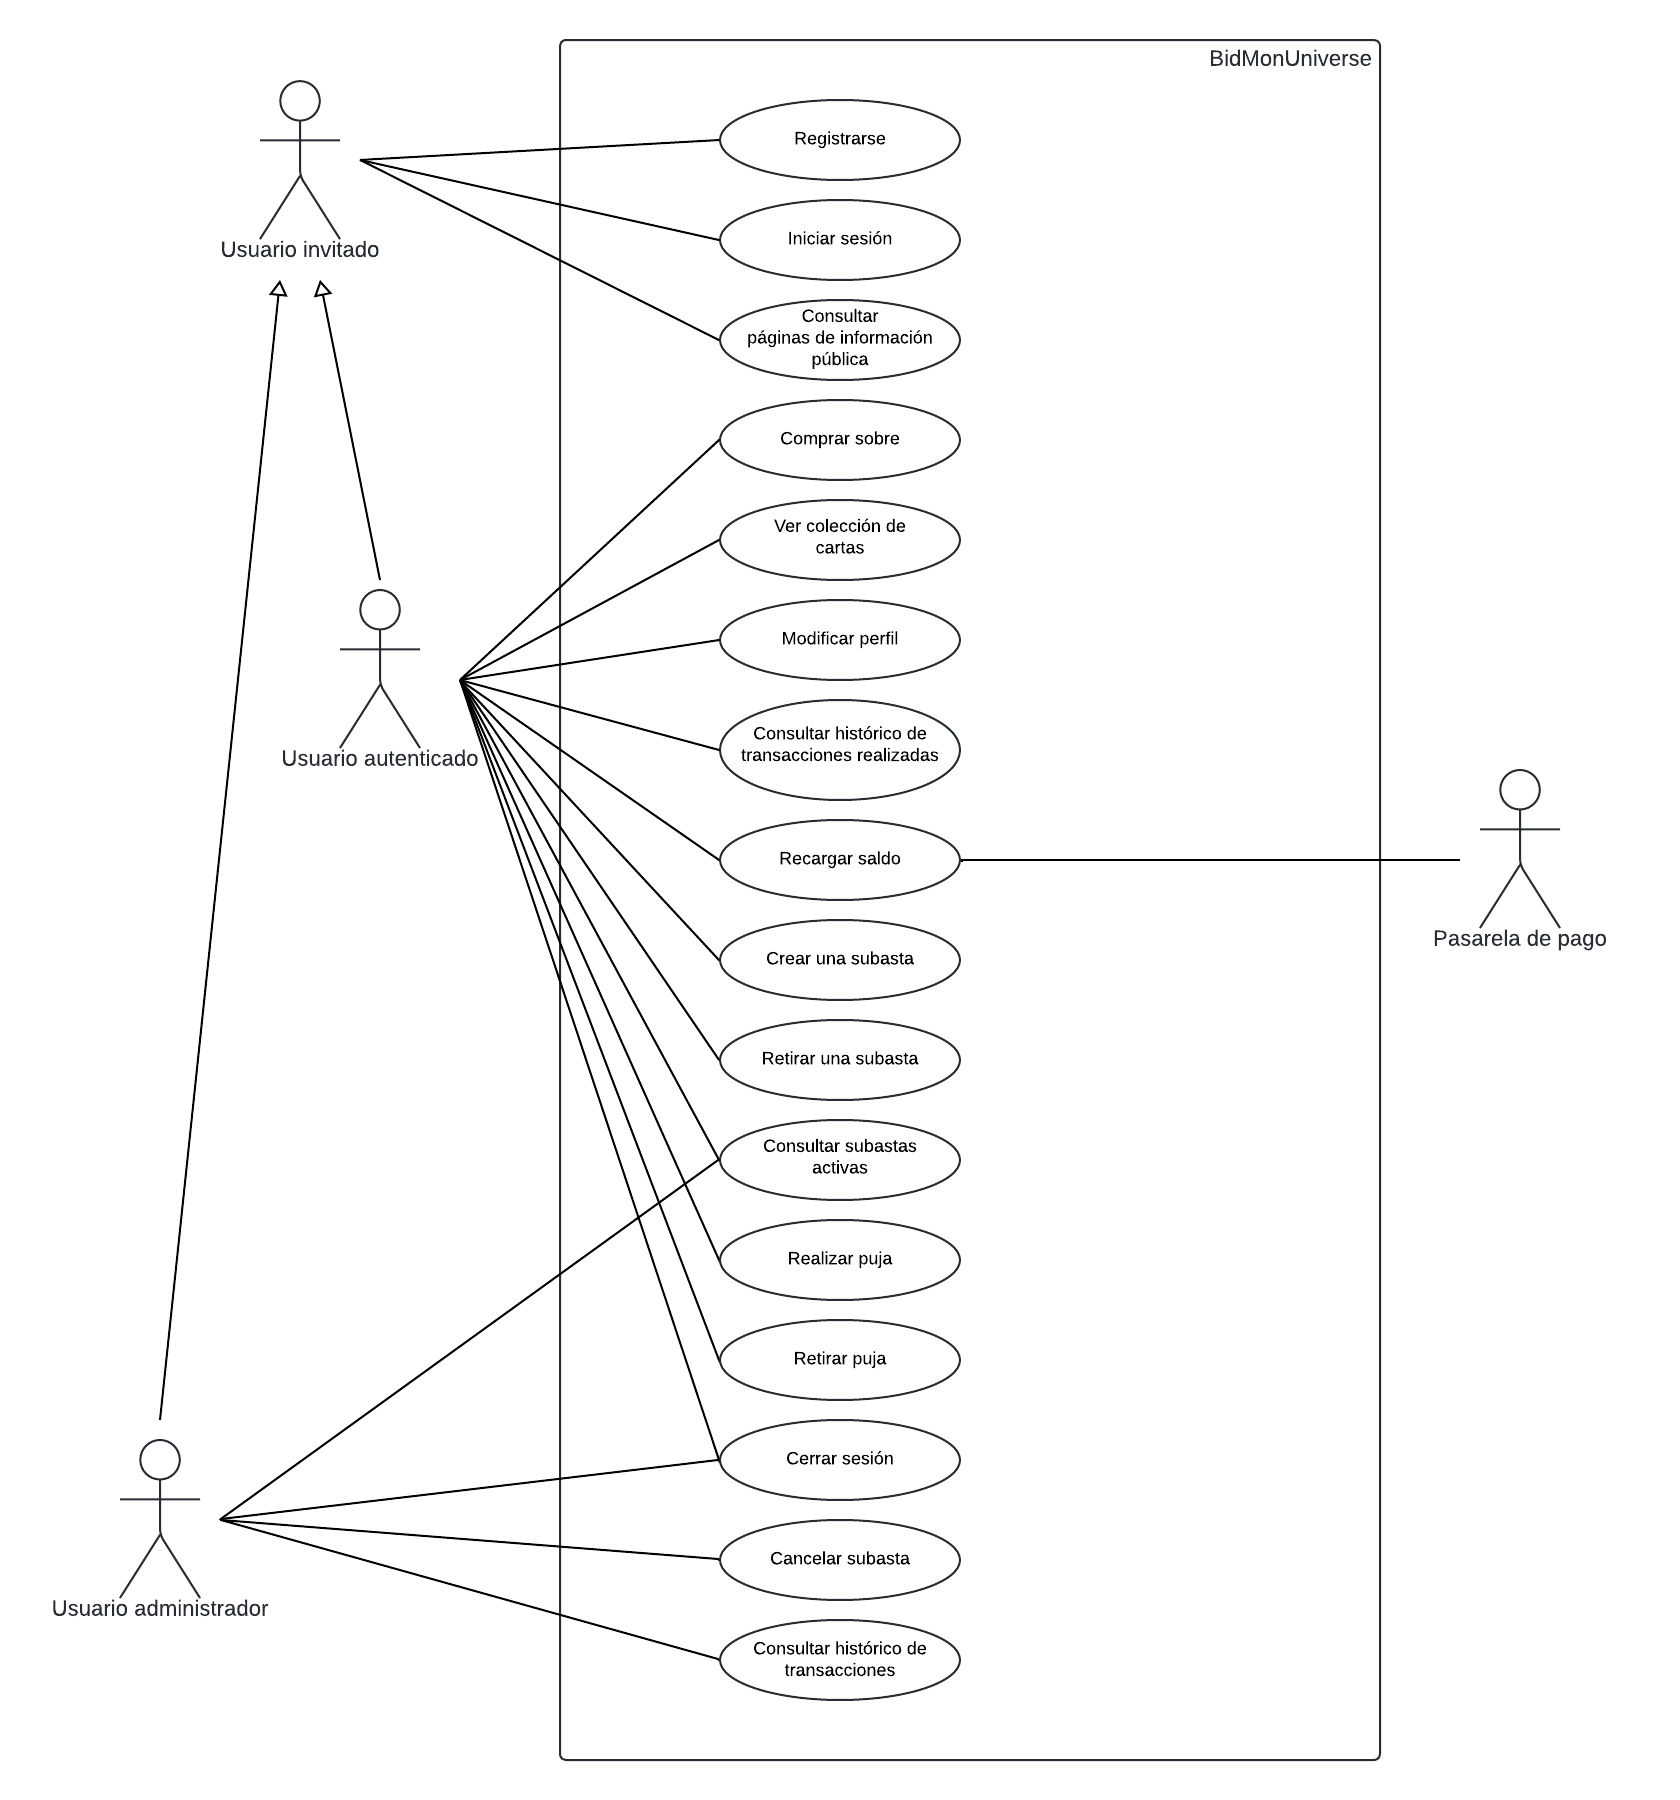
\includegraphics[width=1\textwidth]{figures/6-Analisis/6-Casos-uso/6_Diagrama-contexto.png}
    \caption{Diagrama de contexto del sistema}
    \label{fig:diagrama_contexto}
\end{figure}


\subsection{Casos de uso. Usuario invitado}

\begin{longtable}{
    >{\columncolor{lightgreen!20}}p{4cm}
    p{12cm}
    }
    \caption{Caso de uso. Registro} \label{table:cu_registro} \\
    \toprule
    \rowcolor{darkgreen!50}
    \textbf{Caso de uso} & \multicolumn{1}{>{\columncolor{darkgreen!50}\centering\arraybackslash}p{12cm}}{\textbf{REGISTRO}} \\
    \endfirsthead
    
    \multicolumn{2}{c}%
    {{ \tablename\ \thetable{} Caso de uso. Registro -- continuación de la página anterior}} \\
    \toprule
    \rowcolor{darkgreen!50}
    \textbf{Caso de uso} & \multicolumn{1}{>{\columncolor{darkgreen!50}\centering\arraybackslash}p{12cm}}{\textbf{REGISTRO}} \\
    \midrule
    \endhead
    
    \midrule
    \multicolumn{2}{r}{{Continúa en la siguiente página...}} \\ 
    \endfoot
    
    \bottomrule
    \endlastfoot
    
    \midrule
    Descripción & Un usuario invitado se puede registrar en el sistema para poder acceder a las funcionalidades del mismo. \\
    \midrule
    Actores principales & Usuario invitado \\
    \midrule
    Actores secundarios &  \\
    \midrule
    Precondiciones & El usuario no debe estar registrado en el sistema. \\
    \midrule
    Postcondiciones & \begin{itemize}[nosep,leftmargin=*]
      \item Se crea un nuevo registro en la base de datos con los datos del usuario.
      \item Se notifica al usuario que su registro ha sido exitoso.
      \item Se redirige al usuario a la página de inicio de sesión.
    \end{itemize} \\
    \midrule
    Disparadores & El usuario hace clic en el botón de registro. \\
    \midrule
    Escenario principal & \begin{enumerate}[nosep,leftmargin=*]
      \item El sistema muestra el formulario de registro.
      \item El usuario completa el formulario con sus datos personales.
      \item El usuario hace clic en el botón de registro.
      \item El sistema valida los datos del formulario.
      \item El sistema crea un nuevo registro en la base de datos con los datos del usuario.
      \item El sistema notifica al usuario que su registro ha sido exitoso.
      \item El sistema redirige al usuario a la página de inicio de sesión.
    \end{enumerate} \\
    \midrule
    Escenarios alternativos & 
    \begin{itemize}[nosep,leftmargin=*]
      \item Escenario alternativo 1. El usuario cancela el registro.
      \begin{enumerate}[nosep,leftmargin=*]
          \item El usuario hace clic en otro enlace.
          \item El sistema no crea el registro y redirige al usuario a la página correspondiente.
      \end{enumerate}
      \item Escenario alternativo 2. El usuario ya está registrado en el sistema.
      \begin{enumerate}[nosep,leftmargin=*]
          \item El sistema muestra un mensaje de error.
          \item El sistema no crea el registro y redirige al usuario de nuevo al formulario de registro.
      \end{enumerate}
      \item Escenario alternativo 3. El usuario no completa el formulario correctamente.
      \begin{enumerate}[nosep,leftmargin=*]
          \item El sistema muestra un mensaje de error con los campos que no se han completado correctamente.
          \item El sistema no crea el registro y redirige al usuario de nuevo al formulario de registro.
      \end{enumerate}
    \end{itemize} \\
    \midrule
    Situaciones de error & \begin{itemize}[nosep,leftmargin=*]
      \item Error 1. Error de conexión a la base de datos.
      \begin{enumerate}[nosep,leftmargin=*]
          \item El sistema muestra un mensaje de error.
          \item El sistema redirige al usuario de nuevo al formulario de registro.
      \end{enumerate}
    \end{itemize} \\
    \end{longtable}

\subsection{Casos de uso. Usuario autenticado}

\subsubsection{Caso de uso. Comprar sobre} \label{sec:cu_comprar-sobre}
\begin{longtable}{
    >{\columncolor{lightgreen!20}}p{4cm}
    p{12cm}
    }
    \caption{Caso de uso. Comprar sobre} \label{table:cu_comprar-sobre} \\
    \toprule
    \rowcolor{darkgreen!50}
    \textbf{Caso de uso} & \multicolumn{1}{>{\columncolor{darkgreen!50}\centering\arraybackslash}p{12cm}}{\textbf{COMPRAR SOBRE}} \\
    \endfirsthead
    
    \multicolumn{2}{c}%
    {{ \tablename\ \thetable{} Caso de uso. Comprar sobre -- continuación de la página anterior}} \\
    \toprule
    \rowcolor{darkgreen!50}
    \textbf{Caso de uso} & \multicolumn{1}{>{\columncolor{darkgreen!50}\centering\arraybackslash}p{12cm}}{\textbf{COMPRAR SOBRE}} \\
    \midrule
    \endhead
    
    \midrule
    \multicolumn{2}{r}{{Continúa en la siguiente página...}} \\ 
    \endfoot
    
    \bottomrule
    \endlastfoot
    
    \midrule
    Descripción & Un usuario autenticado puede comprar un sobre de cartas. \\
    \midrule
    Actores principales & Usuario autenticado \\
    \midrule
    Actores secundarios &  \\
    \midrule
    Precondiciones & \begin{itemize}[nosep,leftmargin=*]
        \item El usuario ha iniciado sesión en el sistema.
        \item El usuario dispone de saldo suficiente para comprar el sobre.
    \end{itemize} \\
    \midrule
    Postcondiciones & \begin{itemize}[nosep,leftmargin=*]
        \item Se descuenta el precio del sobre del saldo del usuario.
        \item Se añaden las cartas del sobre a la colección del usuario.
        \item Se decrementa en una unidad la cantidad de sobres disponibles en el inventario.
        \item Se registra la transacción en el historial de compras del usuario.
    \end{itemize} \\
    \midrule
    Disparadores & El usuario hace clic en el botón de comprar sobre. \\
    \midrule
    Escenario principal & \begin{enumerate}[nosep,leftmargin=*]
        \item El sistema muestra el inventario de sobres disponibles.
        \item El usuario selecciona el sobre que desea comprar.
        \item El usuario hace clic en el botón de comprar sobre.
        \item El sistema valida que el usuario dispone de saldo suficiente.
        \item El sistema descuenta el precio del sobre del saldo del usuario.
        \item El sistema genera las cartas del sobre.
        \item El sistema añade las cartas del sobre a la colección del usuario.
    \end{enumerate} \\
    \midrule
    Escenarios alternativos & 
    \begin{itemize}[nosep,leftmargin=*]
        \item \textbf{Escenario alternativo 1. El usuario intenta comprar un sobre sin saldo suficiente.}
        \begin{enumerate}[nosep,leftmargin=*]
            \item El usuario intenta comprar un sobre sin saldo suficiente.
            \item El sistema muestra un mensaje de error.
            \item El sistema le ofrece al usuario la posibilidad de recargar saldo.
        \end{enumerate}
    \end{itemize} \\
    \midrule
    Situaciones de error & 
    \begin{itemize}[nosep,leftmargin=*]
        \item \textbf{Error de conexión a la base de datos.}
        \begin{enumerate}[nosep,leftmargin=*]
            \item El sistema muestra un mensaje de error.
            \item El sistema no descuenta el precio del sobre del saldo del usuario.
            \item El sistema no añade las cartas del sobre a la colección del usuario.
            \item El sistema no decrementa en una unidad la cantidad de sobres disponibles en el inventario.
        \end{enumerate}
    \end{itemize} \\
\end{longtable}



\subsubsection{Caso de uso. Ver colección de cartas} \label{sec:cu_coleccion-cartas}
\begin{longtable}{
    >{\columncolor{lightgreen!20}}p{4cm}
    p{12cm}
    }
    \caption{Caso de uso. Ver colección de cartas} \label{table:cu_coleccion-cartas} \\
    \toprule
    \rowcolor{darkgreen!50}
    \textbf{Caso de uso} & \multicolumn{1}{>{\columncolor{darkgreen!50}\centering\arraybackslash}p{12cm}}{\textbf{VER COLECCIÓN DE CARTAS}} \\
    \endfirsthead
    
    \multicolumn{2}{c}%
    {{ \tablename\ \thetable{} Caso de uso. Ver colección de cartas -- continuación de la página anterior}} \\
    \toprule
    \rowcolor{darkgreen!50}
    \textbf{Caso de uso} & \multicolumn{1}{>{\columncolor{darkgreen!50}\centering\arraybackslash}p{12cm}}{\textbf{VER COLECCIÓN DE CARTAS}} \\
    \midrule
    \endhead
    
    \midrule
    \multicolumn{2}{r}{{Continúa en la siguiente página...}} \\ 
    \endfoot
    
    \bottomrule
    \endlastfoot
    
    \midrule
    Descripción & Un usuario autenticado puede ver la colección de cartas que posee. \\
    \midrule
    Actores principales & Usuario autenticado \\
    \midrule
    Actores secundarios &  \\
    \midrule
    Precondiciones & \begin{itemize}[nosep,leftmargin=*]
        \item El usuario debe haber iniciado sesión en el sistema.
    \end{itemize} \\
    \midrule
    Postcondiciones & \\
    \midrule
    Disparadores & El usuario accede a la sección de colección de cartas. \\
    \midrule
    Escenario principal & \begin{enumerate}[nosep,leftmargin=*]
        \item El sistema muestra la colección de cartas del usuario.
        \item El usuario puede seleccionar una carta para ver su información detallada.
    \end{enumerate} \\
    \midrule
    Escenarios alternativos & 
    \begin{itemize}[nosep,leftmargin=*]
        \item \textbf{Escenario alternativo 1. El usuario no tiene cartas en su colección.}
        \begin{enumerate}[nosep,leftmargin=*]
            \item Se mostrará un mensaje indicando que el usuario no tiene cartas en su colección.
            \item Se mostrará la opción de comprar un sobre de cartas o ir a la sección de subastas.
        \end{enumerate}
    \end{itemize} \\
    \midrule
    Situaciones de error & 
    \begin{itemize}[nosep,leftmargin=*]
        \item \textbf{Error de conexión a la base de datos.}
        \begin{enumerate}[nosep,leftmargin=*]
            \item El sistema mostrará un mensaje de error.
            \item El sistema le dará al usuario la opción de intentar cargar de nuevo la colección o volver a la página principal.
        \end{enumerate}
    \end{itemize} \\
\end{longtable}


\subsubsection{Caso de uso. Marcar carta como destacada} \label{sec:cu_carta-destacada}
\begin{longtable}{
    >{\columncolor{lightgreen!20}}p{4cm}
    p{12cm}
    }
    \caption{Caso de uso. Marcar carta como destacada} \label{table:cu_carta-destacada} \\
    \toprule
    \rowcolor{darkgreen!50}
    \textbf{Caso de uso} & \multicolumn{1}{>{\columncolor{darkgreen!50}\centering\arraybackslash}p{12cm}}{\textbf{MARCAR CARTA COMO DESTACADA}} \\
    \endfirsthead
    
    \multicolumn{2}{c}%
    {{ \tablename\ \thetable{} Caso de uso. Marcar carta como destacada -- continuación de la página anterior}} \\
    \toprule
    \rowcolor{darkgreen!50}
    \textbf{Caso de uso} & \multicolumn{1}{>{\columncolor{darkgreen!50}\centering\arraybackslash}p{12cm}}{\textbf{MARCAR CARTA COMO DESTACADA}} \\
    \midrule
    \endhead
    
    \midrule
    \multicolumn{2}{r}{{Continúa en la siguiente página...}} \\ 
    \endfoot
    
    \bottomrule
    \endlastfoot
    
    \midrule
    Descripción & Un usuario autenticado puede marcar una carta de su colección como destacada. \\
    \midrule
    Actores principales & Usuario autenticado \\
    \midrule
    Actores secundarios &  \\
    \midrule
    Precondiciones & \begin{itemize}[nosep,leftmargin=*]
        \item El usuario debe haber iniciado sesión en el sistema.
        \item El usuario debe tener al menos una carta en su colección.
    \end{itemize} \\
    \midrule
    Postcondiciones & \begin{itemize}[nosep,leftmargin=*]
        \item Se marca la carta como destacada en la base de datos.
    \end{itemize} \\
    \midrule
    Disparadores & El usuario accede a la sección de colección de cartas, selecciona una carta y la marca como destacada. \\
    \midrule
    Escenario principal & \begin{enumerate}[nosep,leftmargin=*]
        \item El sistema muestra la colección de cartas del usuario.
        \item El usuario puede seleccionar una carta para marcarla como destacada.
        \item El usuario hace clic en el botón de marcar como destacada.
        \item El sistema valida que el usuario no tenga ya una carta marcada como destacada.
        \item El sistema marca la carta como destacada en la base de datos.
        \item El sistema muestra un mensaje de éxito.
        \item El sistema redirige al usuario a la página que muestra su colección de cartas.
    \end{enumerate} \\
    \midrule
    Escenarios alternativos & 
    \begin{itemize}[nosep,leftmargin=*]
        \item \textbf{Escenario alternativo 1. El usuario ya tiene una carta marcada como destacada.}
        \begin{enumerate}[nosep,leftmargin=*]
            \item Se mostrará un mensaje indicando que el usuario ya tiene una carta marcada como destacada.
            \item Se mostrará la opción de desmarcar la carta actualmente destacada.
            \item Si el usuario confirma, se desmarcará la carta actualmente destacada y se marcará la nueva carta.
        \end{enumerate}
    \end{itemize} \\
    \midrule
    Situaciones de error & 
    \begin{itemize}[nosep,leftmargin=*]
        \item \textbf{Error de conexión a la base de datos.}
        \begin{enumerate}[nosep,leftmargin=*]
            \item El sistema mostrará un mensaje de error.
            \item El sistema no actualizará la carta como destacada en la base de datos.
            \item El sistema redirigirá al usuario a la página que muestra su colección de cartas.
        \end{enumerate}
    \end{itemize} \\
\end{longtable}




\subsubsection{Caso de uso. Modificar perfil} \label{sec:cu_modificar-perfil}
\begin{longtable}{
    >{\columncolor{lightgreen!20}}p{4cm}
    p{12cm}
    }
    \caption{Caso de uso. Modificar perfil} \label{table:cu_modificar-perfil} \\
    \toprule
    \rowcolor{darkgreen!50}
    \textbf{Caso de uso} & \multicolumn{1}{>{\columncolor{darkgreen!50}\centering\arraybackslash}p{12cm}}{\textbf{MODIFICAR PERFIL}} \\
    \endfirsthead
    
    \multicolumn{2}{c}%
    {{ \tablename\ \thetable{} Caso de uso. Modificar perfil -- continuación de la página anterior}} \\
    \toprule
    \rowcolor{darkgreen!50}
    \textbf{Caso de uso} & \multicolumn{1}{>{\columncolor{darkgreen!50}\centering\arraybackslash}p{12cm}}{\textbf{MODIFICAR PERFIL}} \\
    \midrule
    \endhead
    
    \midrule
    \multicolumn{2}{r}{{Continúa en la siguiente página...}} \\ 
    \endfoot
    
    \bottomrule
    \endlastfoot
    
    \midrule
    Descripción & Un usuario autenticado puede modificar su perfil de usuario. \\
    \midrule
    Actores principales & Usuario autenticado \\
    \midrule
    Actores secundarios &  \\
    \midrule
    Precondiciones & \begin{itemize}[nosep,leftmargin=*]
        \item El usuario debe haber iniciado sesión en el sistema.
    \end{itemize} \\
    \midrule
    Postcondiciones & \begin{itemize}[nosep,leftmargin=*]
        \item Se modifican los datos del perfil del usuario en la base de datos.
    \end{itemize} \\
    \midrule
    Disparadores & El usuario accede a la sección de modificar perfil. \\
    \midrule
    Escenario principal & \begin{enumerate}[nosep,leftmargin=*]
        \item El sistema muestra el formulario de modificación de perfil.
        \item El usuario modifica los campos que desee.
        \item El usuario hace clic en el botón de guardar cambios.
        \item El sistema valida los campos del formulario.
        \item El sistema actualiza los datos del perfil del usuario.
        \item El sistema muestra un mensaje de éxito.
        \item El sistema redirige al usuario a la página que muestra su perfil.
    \end{enumerate} \\
    \midrule
    Escenarios alternativos & 
    \begin{itemize}[nosep,leftmargin=*]
        \item \textbf{Escenario alternativo 1. El usuario cancela la modificación de perfil.}
        \begin{enumerate}[nosep,leftmargin=*]
            \item El usuario hace clic en el botón de cancelar.
            \item El sistema no modifica los datos del perfil del usuario.
            \item El sistema redirige al usuario a la página que muestra su perfil.
        \end{enumerate}
        \item \textbf{Escenario alternativo 2. El usuario introduce datos inválidos.}
        \begin{enumerate}[nosep,leftmargin=*]
            \item El sistema muestra un mensaje de error.
            \item El sistema no modifica los datos del perfil del usuario.
            \item El sistema muestra los campos con errores.
            \item El sistema permite al usuario corregir los errores.
        \end{enumerate}
    \end{itemize} \\
    \midrule
    Situaciones de error & 
    \begin{itemize}[nosep,leftmargin=*]
        \item \textbf{Error de conexión a la base de datos.}
        \begin{enumerate}[nosep,leftmargin=*]
            \item El sistema mostrará un mensaje de error.
            \item El sistema no modificará los datos del perfil del usuario.
            \item El sistema le dará al usuario la opción de intentar guardar de nuevo los cambios o volver a la página que muestra su perfil.
        \end{enumerate}
    \end{itemize} \\
\end{longtable}




\subsubsection{Caso de uso. Histórico de transacciones realizadas} \label{sec:cu_transacciones-realizadas}
\begin{longtable}{
    >{\columncolor{lightgreen!20}}p{4cm}
    >{\columncolor{white}}p{12cm} 
    }
    \caption{Caso de uso. Histórico de transacciones realizadas} \label{table:cu_transacciones-realizadas} \\
    \toprule
    \rowcolor{darkgreen!50}
    \textbf{Caso de uso} & \multicolumn{1}{>{\columncolor{darkgreen!50}\centering\arraybackslash}p{12cm}}{\textbf{HISTÓRICO DE TRANSACCIONES REALIZADAS}} \\
    \endfirsthead
    
    \multicolumn{2}{c}%
    {{ \tablename\ \thetable{} Caso de uso. Histórico de transacciones realizadas -- continuación de la página anterior}} \\
    \toprule
    \rowcolor{darkgreen!50}
    \textbf{Caso de uso} & \multicolumn{1}{>{\columncolor{darkgreen!50}\centering\arraybackslash}p{12cm}}{\textbf{HISTÓRICO DE TRANSACCIONES REALIZADAS}} \\
    \midrule
    \endhead
    
    \midrule
    \multicolumn{2}{r}{{Continúa en la siguiente página...}} \\ 
    \endfoot
    
    \bottomrule
    \endlastfoot
    
    \midrule
    Descripción & Un usuario autenticado puede consultar el histórico de transacciones realizadas en el sistema. \\
    \midrule
    Actores principales & Usuario autenticado \\
    \midrule
    Actores secundarios &  \\
    \midrule
    Precondiciones & \begin{itemize}[nosep,leftmargin=*]
        \item El usuario debe haber iniciado sesión en el sistema.
    \end{itemize} \\
    \midrule
    Postcondiciones & \\
    \midrule
    Disparadores & El usuario accede a la sección de historial de transacciones. \\
    \midrule
    Escenario principal & \begin{enumerate}[nosep,leftmargin=*]
        \item El sistema muestra el historial de transacciones del usuario.
    \end{enumerate} \\
    \midrule
    Escenarios alternativos & 
    \begin{itemize}[nosep,leftmargin=*]
        \item \textbf{Escenario alternativo 1. El usuario no tiene transacciones realizadas.}
        \begin{enumerate}[nosep,leftmargin=*]
            \item El sistema mostrará un mensaje indicando que el usuario no tiene transacciones realizadas.
        \end{enumerate}
    \end{itemize} \\
    \midrule
    Situaciones de error & 
    \begin{itemize}[nosep,leftmargin=*]
        \item \textbf{Error de conexión a la base de datos.}
        \begin{enumerate}[nosep,leftmargin=*]
            \item El sistema mostrará un mensaje de error.
            \item El sistema le dará al usuario la opción de intentar cargar de nuevo el historial de transacciones o volver a la página principal.
        \end{enumerate}
    \end{itemize} \\
\end{longtable}




\subsubsection{Caso de uso. Recargar saldo} \label{sec:cu_recarga-saldo}
\begin{longtable}{
    >{\columncolor{lightgreen!20}}p{4cm}
    p{12cm}
    }
    \caption{Caso de uso. Recargar saldo} \label{table:cu_recarga-saldo} \\
    \toprule
    \rowcolor{darkgreen!50}
    \textbf{Caso de uso} & \multicolumn{1}{>{\columncolor{darkgreen!50}\centering\arraybackslash}p{12cm}}{\textbf{RECRAGAR SALDO}} \\
    \endfirsthead
    
    \multicolumn{2}{c}%
    {{ \tablename\ \thetable{} Caso de uso. Recargar saldo -- continuación de la página anterior}} \\
    \toprule
    \rowcolor{darkgreen!50}
    \textbf{Caso de uso} & \multicolumn{1}{>{\columncolor{darkgreen!50}\centering\arraybackslash}p{12cm}}{\textbf{RECARGAR SALDO}} \\
    \midrule
    \endhead
    
    \midrule
    \multicolumn{2}{r}{{Continúa en la siguiente página...}} \\ 
    \endfoot
    
    \bottomrule
    \endlastfoot
    
    \midrule
    Descripción & Un usuario autenticado puede recargar saldo en su cuenta. \\
    \midrule
    Actores principales & Usuario autenticado \\
    \midrule
    Actores secundarios &  Pasarela de pago \\
    \midrule
    Precondiciones & \begin{itemize}[nosep,leftmargin=*]
        \item El usuario debe haber iniciado sesión en el sistema.
    \end{itemize} \\
    \midrule
    Postcondiciones & \begin{itemize}[nosep,leftmargin=*]
        \item Se incrementa el saldo del usuario en la base de datos.
    \end{itemize} \\
    \midrule
    Disparadores & El usuario accede a la sección de recarga de saldo. \\
    \midrule
    Escenario principal & \begin{enumerate}[nosep,leftmargin=*]
        \item El sistema muestra el formulario de recarga de saldo.
        \item El usuario introduce la cantidad de saldo que desea recargar.
        \item El usuario hace clic en el botón de recargar saldo.
        \item El sistema valida la cantidad de saldo introducida.
        \item El sistema redirige al usuario a la pasarela de pago.
        \item El usuario completa el pago.
        \item El sistema incrementa el saldo del usuario en la base de datos.
        \item El sistema muestra un mensaje de éxito.
    \end{enumerate} \\
    \midrule
    Escenarios alternativos & 
    \begin{itemize}[nosep,leftmargin=*]
        \item \textbf{Escenario alternativo 1. El usuario cancela la recarga de saldo en la pasarela de pago.}
        \begin{enumerate}[nosep,leftmargin=*]
            \item El usuario cancela el pago.
            \item El sistema no incrementa el saldo del usuario en la base de datos.
            \item El sistema redirige al usuario a la página que muestra su saldo actual.
            \item El sistema muestra un mensaje de cancelación.
        \end{enumerate}
        \item \textbf{Escenario alternativo 2. El usuario introduce una cantidad de saldo inválida.}
        \begin{enumerate}[nosep,leftmargin=*]
            \item El sistema muestra un mensaje de error.
            \item El sistema muestra los campos con errores.
            \item El sistema permite al usuario corregir los errores.
        \end{enumerate}
    \end{itemize} \\
    \midrule
    Situaciones de error & 
    \begin{itemize}[nosep,leftmargin=*]
        \item \textbf{Error de conexión a la base de datos.}
        \begin{enumerate}[nosep,leftmargin=*]
            \item El sistema mostrará un mensaje de error.
            \item El sistema no incrementará el saldo del usuario en la base de datos.
            \item El sistema le dará al usuario la opción de intentar recargar de nuevo el saldo o volver a la página de inicio.
        \end{enumerate}
        \item \textbf{Error en la pasarela de pago.}
        \begin{enumerate}[nosep,leftmargin=*]
            \item El sistema mostrará un mensaje de error.
            \item El sistema no incrementará el saldo del usuario en la base de datos.
            \item El sistema redirigirá al usuario a la página de recarga de saldo.
        \end{enumerate}
    \end{itemize} \\
\end{longtable}



\subsubsection{Caso de uso. Crear una subasta} \label{sec:cu_crear-subasta}
\begin{longtable}{
    >{\columncolor{lightgreen!20}}p{4cm}
    p{12cm}
    }
    \caption{Caso de uso. Crear una subasta} \label{table:cu_crear-subasta} \\
    \toprule
    \rowcolor{darkgreen!50}
    \textbf{Caso de uso} & \multicolumn{1}{>{\columncolor{darkgreen!50}\centering\arraybackslash}p{12cm}}{\textbf{CREAR UNA SUBASTA}} \\
    \endfirsthead
    
    \multicolumn{2}{c}%
    {{ \tablename\ \thetable{} Caso de uso. Crear una subasta -- continuación de la página anterior}} \\
    \toprule
    \rowcolor{darkgreen!50}
    \textbf{Caso de uso} & \multicolumn{1}{>{\columncolor{darkgreen!50}\centering\arraybackslash}p{12cm}}{\textbf{CREAR UNA SUBASTA}} \\
    \midrule
    \endhead
    
    \midrule
    \multicolumn{2}{r}{{Continúa en la siguiente página...}} \\ 
    \endfoot
    
    \bottomrule
    \endlastfoot
    
    \midrule
    Descripción & Un usuario autenticado puede crear una subasta de una carta de su colección. \\
    \midrule
    Actores principales & Usuario autenticado \\
    \midrule
    Actores secundarios &  \\
    \midrule
    Precondiciones & \begin{itemize}[nosep,leftmargin=*]
        \item El usuario debe haber iniciado sesión en el sistema.
        \item El usuario debe tener al menos una carta en su colección.
        \item El usuario no debe tener ya una subasta activa para la carta que desea subastar.
    \end{itemize} \\
    \midrule
    Postcondiciones & \begin{itemize}[nosep,leftmargin=*]
        \item Se crea una nueva subasta en la base de datos.
        \item Se marca la carta como 'en subasta' en la base de datos.
    \end{itemize} \\
    \midrule
    Disparadores & El usuario accede a la sección de subastas y hace clic en el botón de crear subasta. \\
    \midrule
    Escenario principal & \begin{enumerate}[nosep,leftmargin=*]
        \item El sistema muestra el formulario de creación de subasta.
        \item El usuario selecciona la carta que desea subastar.
        \item El usuario introduce el precio de salida y la duración de la subasta.
        \item El usuario hace clic en el botón de crear subasta.
        \item El sistema valida los campos del formulario.
        \item El sistema crea una nueva subasta en la base de datos.
        \item El sistema marca la carta como 'en subasta' en la base de datos.
        \item El sistema muestra un mensaje de éxito.
        \item El sistema redirige al usuario a la página de subastas.
        \item El sistema muestra la subasta creada en la lista de subastas.
    \end{enumerate} \\
    \midrule
    Escenarios alternativos & 
    \begin{itemize}[nosep,leftmargin=*]
        \item \textbf{Escenario alternativo 1. El usuario ya tiene una subasta activa para la carta que desea subastar.}
        \begin{enumerate}[nosep,leftmargin=*]
            \item El usuario intenta crear una subasta para una carta que ya está en subasta.
            \item El sistema muestra un mensaje de error.
            \item El sistema redirige al usuario a la página de subastas.
        \end{enumerate}
        \item \textbf{Escenario alternativo 2. El usuario introduce datos inválidos.}
        \begin{enumerate}[nosep,leftmargin=*]
            \item El sistema muestra un mensaje de error.
            \item El sistema no crea la subasta en la base de datos.
            \item El sistema no marcará la carta como 'en subasta' en la base de datos.
            \item El sistema le mostrará al usuario los campos con errores.
            \item El sistema permitirá al usuario corregir los errores.
        \end{enumerate}
    \end{itemize} \\
    \midrule
    Situaciones de error & 
    \begin{itemize}[nosep,leftmargin=*]
        \item \textbf{Error de conexión a la base de datos.}
        \begin{enumerate}[nosep,leftmargin=*]
            \item El sistema mostrará un mensaje de error.
            \item El sistema no creará la subasta en la base de datos.
            \item El sistema no marcará la carta como 'en subasta' en la base de datos.
            \item El sistema redirigirá al usuario a la página de subastas.
        \end{enumerate}
    \end{itemize} \\
\end{longtable}




\subsubsection{Caso de uso. Retirar una subasta} \label{sec:cu_retirar-subasta}
\begin{longtable}{
    >{\columncolor{lightgreen!20}}p{4cm}
    p{12cm}
    }
    \caption{Caso de uso. Retirar una subasta} \label{table:cu_retirar-subasta} \\
    \toprule
    \rowcolor{darkgreen!50}
    \textbf{Caso de uso} & \multicolumn{1}{>{\columncolor{darkgreen!50}\centering\arraybackslash}p{12cm}}{\textbf{RETIRAR UNA SUBASTA}} \\
    \endfirsthead
    
    \multicolumn{2}{c}%
    {{ \tablename\ \thetable{} Caso de uso. Retirar una subasta -- continuación de la página anterior}} \\
    \toprule
    \rowcolor{darkgreen!50}
    \textbf{Caso de uso} & \multicolumn{1}{>{\columncolor{darkgreen!50}\centering\arraybackslash}p{12cm}}{\textbf{RETIRAR UNA SUBASTA}} \\
    \midrule
    \endhead
    
    \midrule
    \multicolumn{2}{r}{{Continúa en la siguiente página...}} \\ 
    \endfoot
    
    \bottomrule
    \endlastfoot
    
    \midrule
    Descripción & Un usuario  \\
    \midrule
    Actores principales & Usuario autenticado \\
    \midrule
    Actores secundarios &  \\
    \midrule
    Precondiciones & \begin{itemize}[nosep,leftmargin=*]
        \item El usuario debe haber iniciado sesión en el sistema.
        \item El usuario debe tener al menos una subasta activa.
    \end{itemize} \\
    \midrule
    Postcondiciones & \begin{itemize}[nosep,leftmargin=*]
        \item Se marca la subasta como 'cancelada' en la base de datos.
        \item La carta subastada vuelve a estar disponible en la colección del usuario.
        \item Se actualizan las pujas de la subasta en la base de datos, marcando las pujas como 'canceladas'.
        \item Se informa a los usuarios que hayan pujado en la subasta de que ha sido cancelada.
    \end{itemize} \\
    \midrule
    Disparadores & El usuario accede a la sección de subastas y hace clic en el botón de retirar subasta. \\
    \midrule
    Escenario principal & \begin{enumerate}[nosep,leftmargin=*]
        \item El sistema muestra la lista de subastas activas del usuario.
        \item El usuario selecciona la subasta que desea retirar.
        \item El usuario hace clic en el botón de retirar subasta.
        \item El sistema muestra un mensaje de confirmación.
        \item El usuario confirma la retirada de la subasta.
        \item El sistema marca la subasta como 'cancelada' en la base de datos.
        \item La carta subastada vuelve a estar disponible en la colección del usuario.
        \item El sistema muestra un mensaje de éxito.
        \item El sistema redirige al usuario a la página de subastas.
    \end{enumerate} \\
    \midrule
    Escenarios alternativos & 
    \begin{itemize}[nosep,leftmargin=*]
        \item \textbf{Escenario alternativo 1. El usuario cancela la retirada de la subasta.}
        \begin{enumerate}[nosep,leftmargin=*]
            \item El usuario hace clic en el botón de cancelar en el mensaje de confirmación.
            \item El sistema no marcará la subasta como 'cancelada' en la base de datos.
            \item El sistema redirigirá al usuario a la página de subastas.
        \end{enumerate}
    \end{itemize} \\
    \midrule
    Situaciones de error & 
    \begin{itemize}[nosep,leftmargin=*]
        \item \textbf{Error de conexión a la base de datos.}
        \begin{enumerate}[nosep,leftmargin=*]
            \item El sistema mostrará un mensaje de error.
            \item El sistema no marcará la subasta como 'cancelada' en la base de datos.
            \item El sistema no devolverá la carta subastada a la colección del usuario.
            \item El sistema redirigirá al usuario a la página de subastas.
        \end{enumerate}
    \end{itemize} \\
\end{longtable}




\subsubsection{Caso de uso. Consultar subastas activas} \label{sec:cu_consultar-subastas}
\begin{longtable}{
    >{\columncolor{lightgreen!20}}p{4cm}
    p{12cm}
    }
    \caption{Caso de uso. Consultar subastas activas} \label{table:cu_consultar-subastas} \\
    \toprule
    \rowcolor{darkgreen!50}
    \textbf{Caso de uso} & \multicolumn{1}{>{\columncolor{darkgreen!50}\centering\arraybackslash}p{12cm}}{\textbf{CONSULTAR SUBASTAS ACTIVAS}} \\
    \endfirsthead
    
    \multicolumn{2}{c}%
    {{ \tablename\ \thetable{} Caso de uso. Consultar subastas activas -- continuación de la página anterior}} \\
    \toprule
    \rowcolor{darkgreen!50}
    \textbf{Caso de uso} & \multicolumn{1}{>{\columncolor{darkgreen!50}\centering\arraybackslash}p{12cm}}{\textbf{CONSULTAR SUBASTAS ACTIVAS}} \\
    \midrule
    \endhead
    
    \midrule
    \multicolumn{2}{r}{{Continúa en la siguiente página...}} \\ 
    \endfoot
    
    \bottomrule
    \endlastfoot
    
    \midrule
    Descripción & Un usuario  \\
    \midrule
    Actores principales & Usuario autenticado o usuario administrador \\
    \midrule
    Actores secundarios &  \\
    \midrule
    Precondiciones & \begin{itemize}[nosep,leftmargin=*]
        \item El usuario debe haber iniciado sesión en el sistema.
    \end{itemize} \\
    \midrule
    Postcondiciones &  \\
    \midrule
    Disparadores & El usuario accede a la sección de subastas. \\
    \midrule
    Escenario principal & \begin{enumerate}[nosep,leftmargin=*]
        \item El sistema muestra la lista de subastas activas.
        \item El usuario puede seleccionar una subasta para ver su información detallada.
    \end{enumerate} \\
    \midrule
    Escenarios alternativos & 
    \begin{itemize}[nosep,leftmargin=*]
        \item \textbf{Escenario alternativo 1. No hay subastas activas.}
        \begin{enumerate}[nosep,leftmargin=*]
            \item El sistema mostrará un mensaje indicando que no hay subastas activas.
        \end{enumerate}
        \item \textbf{Escenario alternativo 2. El usuario consulta sus propias subastas.} 
        \begin{enumerate}[nosep,leftmargin=*]
            \item El usuario accede a la sección de subastas.
            \item El sistema muestra la opción de ver las subastas activas del usuario.
            \item El usuario selecciona la opción de ver sus propias subastas.
            \item El sistema muestra la lista de subastas activas del usuario.
        \end{enumerate}
        \item \textbf{Escenario alternativo 3. Un usuario administrador consulta las subastas activas.}
        \begin{enumerate}[nosep,leftmargin=*]
            \item El usuario administrador accede a la sección de subastas.
            \item El sistema muestra la lista de subastas activas de todos los usuarios.
            \item El usuario administrador puede seleccionar una subasta para ver su información detallada.
            \item El usuario administrador puede seleccionar una subasta para cancelarla.
        \end{enumerate}
    \end{itemize} \\
    \midrule
    Situaciones de error & 
    \begin{itemize}[nosep,leftmargin=*]
        \item \textbf{Error de conexión a la base de datos.}
        \begin{enumerate}[nosep,leftmargin=*]
            \item El sistema mostrará un mensaje de error.
        \end{enumerate}
    \end{itemize} \\
\end{longtable}



\subsubsection{Caso de uso. Realizar puja} \label{sec:cu_realizar-puja}
\begin{longtable}{
    >{\columncolor{lightgreen!20}}p{4cm}
    p{12cm}
    }
    \caption{Caso de uso. Realizar puja} \label{table:cu_realizar-puja} \\
    \toprule
    \rowcolor{darkgreen!50}
    \textbf{Caso de uso} & \multicolumn{1}{>{\columncolor{darkgreen!50}\centering\arraybackslash}p{12cm}}{\textbf{REALIZAR PUJA}} \\
    \endfirsthead
    
    \multicolumn{2}{c}%
    {{ \tablename\ \thetable{} Caso de uso. Realizar puja -- continuación de la página anterior}} \\
    \toprule
    \rowcolor{darkgreen!50}
    \textbf{Caso de uso} & \multicolumn{1}{>{\columncolor{darkgreen!50}\centering\arraybackslash}p{12cm}}{\textbf{REALIZAR PUJA}} \\
    \midrule
    \endhead
    
    \midrule
    \multicolumn{2}{r}{{Continúa en la siguiente página...}} \\ 
    \endfoot
    
    \bottomrule
    \endlastfoot
    
    \midrule
    Descripción & Un usuario autenticado puede realizar una puja en una subasta activa. \\
    \midrule
    Actores principales & Usuario autenticado \\
    \midrule
    Actores secundarios &  \\
    \midrule
    Precondiciones & \begin{itemize}[nosep,leftmargin=*]
        \item El usuario debe haber iniciado sesión en el sistema.
        \item El usuario debe tener saldo suficiente para realizar la puja.
    \end{itemize} \\
    \midrule
    Postcondiciones & \begin{itemize}[nosep,leftmargin=*]
        \item Se registra la puja en la base de datos.
    \end{itemize} \\
    \midrule
    Disparadores & El usuario selecciona una subasta activa y hace clic en el botón de realizar puja. \\
    \midrule
    Escenario principal & \begin{enumerate}[nosep,leftmargin=*]
        \item El sistema muestra la información detallada de la subasta.
        \item El usuario introduce la cantidad de la puja.
        \item El usuario hace clic en el botón de realizar puja.
        \item El sistema valida la cantidad de la puja.
        \item El sistema registra la puja en la base de datos.
        \item El sistema muestra un mensaje de éxito.
        \item El sistema muestra un mensaje informativo, indicando que si en el momento de finalización del tiempo de la subasta no cuenta con el saldo suficiente, la puja no será válida.
        \item El sistema redirige al usuario a la página de subastas.
    \end{enumerate} \\
    \midrule
    Escenarios alternativos & 
    \begin{itemize}[nosep,leftmargin=*]
        \item \textbf{Escenario alternativo 1. El usuario no tiene saldo suficiente para realizar la puja.}
        \begin{enumerate}[nosep,leftmargin=*]
            \item El usuario intenta realizar una puja sin tener saldo suficiente.
            \item El sistema mostrará un mensaje de error.
            \item El sistema no registrará la puja en la base de datos.
            \item El sistema redirigirá al usuario a la página de subastas.
        \end{enumerate}
        \item \textbf{Escenario alternativo 2. El usuario introduce una cantidad de puja inválida.}
        \begin{enumerate}[nosep,leftmargin=*]
            \item El sistema mostrará un mensaje de error.
            \item El sistema no registrará la puja en la base de datos.
            \item El sistema le mostrará al usuario los campos con errores.
            \item El sistema permitirá al usuario corregir los errores.
        \end{enumerate}
    \end{itemize} \\
    \midrule
    Situaciones de error & 
    \begin{itemize}[nosep,leftmargin=*]
        \item \textbf{Error de conexión a la base de datos.}
        \begin{enumerate}[nosep,leftmargin=*]
            \item El sistema mostrará un mensaje de error.
            \item El sistema no registrará la puja en la base de datos.
            \item El sistema redirigirá al usuario a la página de subastas.
        \end{enumerate}
    \end{itemize} \\
\end{longtable}



\subsubsection{Caso de uso. Retirar puja} \label{sec:cu_retirar-puja}
\begin{longtable}{
    >{\columncolor{lightgreen!20}}p{4cm}
    p{12cm}
    }
    \caption{Caso de uso. Retirar puja} \label{table:cu_retirar-puja} \\
    \toprule
    \rowcolor{darkgreen!50}
    \textbf{Caso de uso} & \multicolumn{1}{>{\columncolor{darkgreen!50}\centering\arraybackslash}p{12cm}}{\textbf{RETIRAR PUJA}} \\
    \endfirsthead
    
    \multicolumn{2}{c}%
    {{ \tablename\ \thetable{} Caso de uso. Retirar puja -- continuación de la página anterior}} \\
    \toprule
    \rowcolor{darkgreen!50}
    \textbf{Caso de uso} & \multicolumn{1}{>{\columncolor{darkgreen!50}\centering\arraybackslash}p{12cm}}{\textbf{RETIRAR PUJA}} \\
    \midrule
    \endhead
    
    \midrule
    \multicolumn{2}{r}{{Continúa en la siguiente página...}} \\ 
    \endfoot
    
    \bottomrule
    \endlastfoot
    
    \midrule
    Descripción & Un usuario podrá retirar una puja realizada en una subasta activa. \\
    \midrule
    Actores principales & Usuario autenticado \\
    \midrule
    Actores secundarios &  \\
    \midrule
    Precondiciones & \begin{itemize}[nosep,leftmargin=*]
        \item El usuario debe haber iniciado sesión en el sistema.
        \item El usuario debe haber realizado una puja en una subasta activa.
        \item La subasta no debe haber finalizado.
    \end{itemize} \\
    \midrule
    Postcondiciones & \begin{itemize}[nosep,leftmargin=*]
        \item Se actualiza la puja en la base de datos, marcándola como 'retirada'.
        \item La puja no se muestra en la lista de pujas activas del usuario.
        \item La puja no se tendr´a en cuenta en el cálculo de la puja más alta.
    \end{itemize} \\
    \midrule
    Disparadores & El usuario accede a la sección de pujas activas, selecciona una puja y hace clic en el botón de retirar puja. \\
    \midrule
    Escenario principal & \begin{enumerate}[nosep,leftmargin=*]
        \item El sistema muestra la lista de pujas activas del usuario.
        \item El usuario selecciona la puja que desea retirar.
        \item El usuario hace clic en el botón de retirar puja.
        \item El sistema muestra un mensaje de confirmación.
        \item El usuario confirma la retirada de la puja.
        \item El sistema actualiza la puja en la base de datos, marcándola como 'retirada'.
        \item El sistema muestra un mensaje de éxito.
        \item El sistema redirige al usuario a la página de subastas.
    \end{enumerate} \\
    \midrule
    Escenarios alternativos & 
    \begin{itemize}[nosep,leftmargin=*]
        \item \textbf{Escenario alternativo 1. El usuario cancela la retirada de la puja.}
        \begin{enumerate}[nosep,leftmargin=*]
            \item El usuario hace clic en el botón de cancelar en el mensaje de confirmación.
            \item El sistema no marcará la puja como 'retirada' en la base de datos.
            \item El sistema redirigirá al usuario a la página de subastas.
        \end{enumerate}
    \end{itemize} \\
    \midrule
    Situaciones de error & 
    \begin{itemize}[nosep,leftmargin=*]
        \item \textbf{Error de conexión a la base de datos.}
        \begin{enumerate}[nosep,leftmargin=*]
            \item El sistema mostrará un mensaje de error.
            \item El sistema redirigirá al usuario a la página de subastas.
        \end{enumerate}
    \end{itemize} \\
\end{longtable}



\subsubsection{Caso de uso. Consultar pujas activas} \label{sec:cu_consultar-pujas}
\begin{longtable}{
    >{\columncolor{lightgreen!20}}p{4cm}
    p{12cm}
    }
    \caption{Caso de uso. Consultar pujas activas} \label{table:cu_consultar-puja} \\
    \toprule
    \rowcolor{darkgreen!50}
    \textbf{Caso de uso} & \multicolumn{1}{>{\columncolor{darkgreen!50}\centering\arraybackslash}p{12cm}}{\textbf{CONSULTAR PUJAS ACTIVAS}} \\
    \endfirsthead
    
    \multicolumn{2}{c}%
    {{ \tablename\ \thetable{} Caso de uso. Consultar pujas activas -- continuación de la página anterior}} \\
    \toprule
    \rowcolor{darkgreen!50}
    \textbf{Caso de uso} & \multicolumn{1}{>{\columncolor{darkgreen!50}\centering\arraybackslash}p{12cm}}{\textbf{CONSULTAR PUJAS ACTIVAS}} \\
    \midrule
    \endhead
    
    \midrule
    \multicolumn{2}{r}{{Continúa en la siguiente página...}} \\ 
    \endfoot
    
    \bottomrule
    \endlastfoot
    
    \midrule
    Descripción & Un usuario  \\
    \midrule
    Actores principales & Usuario autenticado \\
    \midrule
    Actores secundarios &  \\
    \midrule
    Precondiciones & \begin{itemize}[nosep,leftmargin=*]
        \item El usuario debe haber iniciado sesión en el sistema.
    \end{itemize} \\
    \midrule
    Postcondiciones & \\
    \midrule
    Disparadores & El usuario accede a la sección de subastas y hace clic en el botón de ver pujas activas. \\
    \midrule
    Escenario principal & \begin{enumerate}[nosep,leftmargin=*]
        \item El sistema muestra la lista de pujas activas del usuario.
    \end{enumerate} \\
    \midrule
    Escenarios alternativos & 
    \begin{itemize}[nosep,leftmargin=*]
        \item \textbf{Escenario alternativo 1. No hay pujas activas.}
        \begin{enumerate}[nosep,leftmargin=*]
            \item El sistema mostrará un mensaje indicando que no hay pujas activas.
        \end{enumerate}
    \end{itemize} \\
    \midrule
    Situaciones de error & 
    \begin{itemize}[nosep,leftmargin=*]
        \item \textbf{Error de conexión a la base de datos.}
        \begin{enumerate}[nosep,leftmargin=*]
            \item El sistema mostrará un mensaje de error.
        \end{enumerate}
    \end{itemize} \\
\end{longtable}



\subsubsection{Caso de uso. Cerrar sesión} \label{sec:cu_cerrar-sesion}
\begin{longtable}{
    >{\columncolor{lightgreen!20}}p{4cm}
    p{12cm}
    }
    \caption{Caso de uso. Cerrar sesión} \label{table:cu_cerrar-sesion} \\
    \toprule
    \rowcolor{darkgreen!50}
    \textbf{Caso de uso} & \multicolumn{1}{>{\columncolor{darkgreen!50}\centering\arraybackslash}p{12cm}}{\textbf{CERRAR SESIÓN}} \\
    \endfirsthead
    
    \multicolumn{2}{c}%
    {{ \tablename\ \thetable{} Caso de uso. Cerrar sesión -- continuación de la página anterior}} \\
    \toprule
    \rowcolor{darkgreen!50}
    \textbf{Caso de uso} & \multicolumn{1}{>{\columncolor{darkgreen!50}\centering\arraybackslash}p{12cm}}{\textbf{CERRAR SESIÓN}} \\
    \midrule
    \endhead
    
    \midrule
    \multicolumn{2}{r}{{Continúa en la siguiente página...}} \\ 
    \endfoot
    
    \bottomrule
    \endlastfoot
    
    \midrule
    Descripción & Un usuario puede cerrar sesión en el sistema si previamente ha iniciado sesión. \\
    \midrule
    Actores principales & Usuario autenticado o usuario administrador \\
    \midrule
    Actores secundarios &  \\
    \midrule
    Precondiciones & \begin{itemize}[nosep,leftmargin=*]
        \item El usuario debe haber iniciado sesión en el sistema.
    \end{itemize} \\
    \midrule
    Postcondiciones & \begin{itemize}[nosep,leftmargin=*]
        \item Se elimina la sesión del usuario.
    \end{itemize} \\
    \midrule
    Disparadores & El usuario hace clic en el botón de cerrar sesión. \\
    \midrule
    Escenario principal & \begin{enumerate}[nosep,leftmargin=*]
        \item El usuario hace clic en el botón de cerrar sesión.
        \item El sistema elimina la sesión del usuario.
        \item El sistema redirige al usuario a la página de inicio.
    \end{enumerate} \\
    \midrule
    Escenarios alternativos &  \\
    \midrule
    Situaciones de error &  \\
\end{longtable}

\subsection{Casos de uso. Usuario administrador}

\subsubsection{Caso de uso. Histórico de transacciones del sistema} \label{sec:cu_transacciones-sistema}
\begin{longtable}{
    >{\columncolor{lightgreen!20}}p{4cm}
    p{12cm}
    }
    \caption{Caso de uso. Histórico de transacciones del sistema} \label{table:cu_transacciones-sistema} \\
    \toprule
    \rowcolor{darkgreen!50}
    \textbf{Caso de uso} & \multicolumn{1}{>{\columncolor{darkgreen!50}\centering\arraybackslash}p{12cm}}{\textbf{HISTÓRICO DE TRANSACCIONES DEL SISTEMA}} \\
    \endfirsthead
    
    \multicolumn{2}{c}%
    {{ \tablename\ \thetable{} Caso de uso. Histórico de transacciones del sistema -- continuación de la página anterior}} \\
    \toprule
    \rowcolor{darkgreen!50}
    \textbf{Caso de uso} & \multicolumn{1}{>{\columncolor{darkgreen!50}\centering\arraybackslash}p{12cm}}{\textbf{HISTÓRICO DE TRANSACCIONES DEL SISTEMA}} \\
    \midrule
    \endhead
    
    \midrule
    \multicolumn{2}{r}{{Continúa en la siguiente página...}} \\ 
    \endfoot
    
    \bottomrule
    \endlastfoot
    
    \midrule
    Descripción & Un usuario administrador puede consultar el histórico de transacciones del sistema. \\
    \midrule
    Actores principales & Usuario administrador \\
    \midrule
    Actores secundarios &  \\
    \midrule
    Precondiciones & \begin{itemize}[nosep,leftmargin=*]
        \item El usuario ha iniciado sesión en el sistema.
    \end{itemize} \\
    \midrule
    Postcondiciones &  \\
    \midrule
    Disparadores & El usuario selecciona la opción de consultar el histórico de transacciones. \\
    \midrule
    Escenario principal & \begin{enumerate}[nosep,leftmargin=*]
        \item El sistema muestra el listado de transacciones realizadas en el sistema por los diferentes usuarios.
    \end{enumerate} \\
    \midrule
    Escenarios alternativos & 
    \begin{itemize}[nosep,leftmargin=*]
        \item \textbf{Escenario alternativo 1. No hay transacciones registradas.}
        \begin{enumerate}[nosep,leftmargin=*]
            \item El sistema muestra un mensaje indicando que no hay transacciones registradas.
        \end{enumerate}
    \end{itemize} \\
    \midrule
    Situaciones de error & 
    \begin{itemize}[nosep,leftmargin=*]
        \item \textbf{Error de conexión a la base de datos.}
        \begin{enumerate}[nosep,leftmargin=*]
            \item El sistema muestra un mensaje de error.
        \end{enumerate}
    \end{itemize} \\
\end{longtable}



\subsubsection{Caso de uso. Cancelar subasta activa} \label{sec:cu_cancelar-subasta}
\begin{longtable}{
    >{\columncolor{lightgreen!20}}p{4cm}
    p{12cm}
    }
    \caption{Caso de uso. Cancelar subasta activa} \label{table:cu_cancelar-subasta} \\
    \toprule
    \rowcolor{darkgreen!50}
    \textbf{Caso de uso} & \multicolumn{1}{>{\columncolor{darkgreen!50}\centering\arraybackslash}p{12cm}}{\textbf{CANCELAR SUBASTA ACTIVA}} \\
    \endfirsthead
    
    \multicolumn{2}{c}%
    {{ \tablename\ \thetable{} Caso de uso. Cancelar subasta activa -- continuación de la página anterior}} \\
    \toprule
    \rowcolor{darkgreen!50}
    \textbf{Caso de uso} & \multicolumn{1}{>{\columncolor{darkgreen!50}\centering\arraybackslash}p{12cm}}{\textbf{CANCELAR SUBASTA ACTIVA}} \\
    \midrule
    \endhead
    
    \midrule
    \multicolumn{2}{r}{{Continúa en la siguiente página...}} \\ 
    \endfoot
    
    \bottomrule
    \endlastfoot
    
    \midrule
    Descripción & Un usuario administrador puede cancelar una subasta activa en el sistema. \\
    \midrule
    Actores principales & Usuario administrador \\
    \midrule
    Actores secundarios &  \\
    \midrule
    Precondiciones & \begin{itemize}[nosep,leftmargin=*]
        \item El usuario ha iniciado sesión en el sistema.
        \item Existe una subasta activa en el sistema.
    \end{itemize} \\
    \midrule
    Postcondiciones & \begin{itemize}[nosep,leftmargin=*]
        \item Se actualiza el estado de la subasta a cancelada en la base de datos.
        \item Se actualizan las pujas realizadas en la subasta cancelada en la base de datos, marcándolas como 'canceladas'.
        \item Se notifica a los usuarios participantes en la subasta de la cancelación.
    \end{itemize} \\
    \midrule
    Disparadores & El usuario selecciona la opción de cancelar una subasta activa. \\
    \midrule
    Escenario principal & \begin{enumerate}[nosep,leftmargin=*]
        \item El sistema muestra el listado de subastas activas en el sistema.
        \item El usuario selecciona la subasta que desea cancelar.
        \item El sistema muestra un mensaje de confirmación de la cancelación.
        \item El usuario confirma la cancelación de la subasta.
        \item El sistema actualiza el estado de la subasta a cancelada en la base de datos.
        \item El sistema actualiza las pujas realizadas en la subasta cancelada en la base de datos, marcándolas como 'canceladas'.
        \item El sistema notifica a los usuarios participantes en la subasta de la cancelación.
        \item El sistema redirige al usuario al listado de subastas activas.
    \end{enumerate} \\
    \midrule
    Escenarios alternativos & \\
    \midrule
    Situaciones de error & 
    \begin{itemize}[nosep,leftmargin=*]
        \item \textbf{Error de conexión a la base de datos.}
        \begin{enumerate}[nosep,leftmargin=*]
            \item El sistema muestra un mensaje de error.
        \end{enumerate}
    \end{itemize} \\
\end{longtable}

\newpage
\section{IDENTIFICACIÓN DE SUBSISTEMAS DE ANÁLISIS}

\subsection{Descripción de los Subsistemas} 

\subsection{Descripción de los Interfaces entre Subsistemas}


\newpage
\section{ANÁLISIS DE LOS CASOS DE USO}

\subsection{Caso de Uso 1} 

\textcolor[rgb]{0.65,0.16,0}{Ejemplo de tabla para análisis de casos de usos}

\begin{table}[H]
  \centering
  \vspace{-5mm}
  \caption{Análisis del Caso de Uso 1}
    \begin{tabular}{p{7.5em}p{24.145em}}
    \toprule
    \rowcolor[rgb]{ .871,  .918,  .965} \multicolumn{2}{p{31.645em}}{\textbf{Registro}} \\
    \midrule
    \rowcolor[rgb]{ .906,  .902,  .902} \textbf{Precondiciones} & \cellcolor[rgb]{ 1,  1,  1}El usuario no debe haber iniciado sesión nunca. \\
    \midrule
    \rowcolor[rgb]{ .906,  .902,  .902} \textbf{Postcondiciones} & \cellcolor[rgb]{ 1,  1,  1}- \\
    \midrule
    \rowcolor[rgb]{ .906,  .902,  .902} \textbf{Actores} & \cellcolor[rgb]{ 1,  1,  1}Usuario no registrado \\
    \midrule
    \rowcolor[rgb]{ .906,  .902,  .902} \textbf{Descripción} & \cellcolor[rgb]{ 1,  1,  1}El usuario accederá a la pantalla principal de la aplicación cuando no se está registrado, y seleccionará el botón de inicio de sesión, que, al ser la primera vez, registrará.Seleccionará la cuenta de Google con la que desee registrarse y el sistema completará el resto del registro. \\
    \midrule
    \rowcolor[rgb]{ .906,  .902,  .902} \textbf{Escenarios          Secundarios} & \cellcolor[rgb]{ 1,  1,  1} El usuario no tiene cuenta de Google: escenario que puede ser posible si accede a la aplicación a través del App Market. En este caso se le solicitará crear una cuenta. \\
    \bottomrule
    \end{tabular}%
\end{table}%
 
\subsection{Caso de Uso 2}



\newpage
\section{ANÁLISIS DE CLASES}

En este apartado se detalla la arquitectura de los subsistemas de análisis. Como se ha visto en el apartado anterior, el sistema se divide en dos subsistemas principales: 
\textbf{restapi} y \textbf{frontend}. El subsistema restapi contiene las clases que implementan la API REST y la lógica de negocio, mientras que el subsistema frontend abarca la interfaz de usuario.

Primero, se presentará el diagrama de paquetes para ofrecer una visión general de la estructura del sistema. Este diagrama ilustrará la organización y 
agrupación de los distintos elementos del sistema en paquetes, permitiendo una comprensión clara de su disposición y jerarquía.

A continuación, se analizará cada subsistema en detalle mediante un diagrama de componentes por cada subsistema. Se ha optado por un diagrama de componentes debido a que el sistema sigue una arquitectura MERN 
(MongoDB, Express, React, Node.js) y este tipo de diagrama aporta más valor que un diagrama de clases al reflejar más fielmente la estructura y relaciones entre los distintos módulos del sistema.

Finalmente, se describirán los componentes identificados en el diagrama, explicando su función específica dentro del sistema y las relaciones que mantienen con otros componentes. 
Esta descripción detallada permitirá entender el papel de cada componente en el funcionamiento global del sistema y cómo colaboran entre sí para cumplir con los objetivos del sistema.

Por último, una vez descritos en detalle cada subsistema, se explicará el diagrama de despliegue. Este diagrama mostrará cómo se distribuyen físicamente los componentes del sistema en el entorno de 
ejecución, especificando las configuraciones de hardware y software necesarias, así como las interconexiones entre los distintos nodos del sistema.


\subsection{Diagrama de paquetes} 
El sistema se divide en dos paquetes principales:
\begin{itemize}
    \item \textbf{restapi}: se corresponde con el \textit{backend} del sistema, contiene las clases que implementan la API REST del sistema y la lógica de negocio.
    \item \textbf{frontend}: se corresponde con el \textit{frontend} del sistema, contiene las clases que implementan la interfaz de usuario.
\end{itemize}

En la \coloredUnderline{\hyperlink{fig:6_5_Diagrama-Paquetes}{Figura \ref*{fig:6_5_Diagrama-Paquetes}: \nameref*{fig:6_5_Diagrama-Paquetes}}} se muestra el diagrama de paquetes del sistema.
\begin{figure}[H]
    \hypertarget{fig:6_5_Diagrama-Paquetes}{}
    \centering
    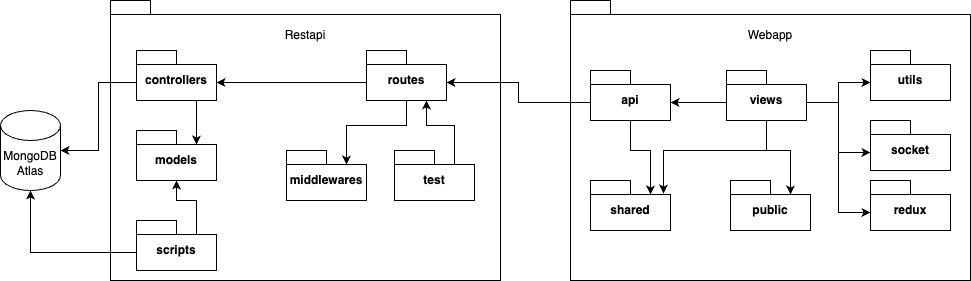
\includegraphics[width=0.8\linewidth]{figures/6-Analisis/6-Clases/6_5-vista_general-paquetes.png}
    \caption{Diagrama de Paquetes del Sistema}
    \label{fig:6_5_Diagrama-Paquetes}
\end{figure}

\subsection{Descripción de los Paquetes}
\subsubsection{restapi}
El paquete \textbf{restapi} contiene las clases que implementan la API REST del sistema y la lógica de negocio. Este paquete se divide en los siguientes subpaquetes:
\begin{itemize}
    \item \textbf{controllers}: contiene las clases que implementan los controladores de la API REST, se encargan de gestionar las peticiones HTTP y las respuestas. Se comunica con la base de datos.
    \item \textbf{models}: contiene las clases que implementan los modelos de datos del sistema.
    \item \textbf{routes}: contiene las clases que implementan las rutas de la API REST, se encargan de definir las rutas y los métodos HTTP asociados.
    \item \textbf{middlewares}: contiene las clases que implementan los middlewares de la API REST, se encargan de gestionar la autenticación y la autorización de los usuarios.
    \item \textbf{scripts}: contiene las clases que implementan los scripts de inicialización de la base de datos.
    \item \textbf{tests}: contiene las clases que implementan las pruebas unitarias de las clases de los otros subpaquetes.
\end{itemize}


\subsubsection{frontend}
El paquete \textbf{frontend} contiene los archivos que implementan la interfaz de usuario. Este paquete se divide en los siguientes subpaquetes:
\begin{itemize} 
    \item \textbf{src}: contiene los archivos que implementan la lógica de la interfaz de usuario.
    \begin{itemize}
        \item \textbf{api}: contiene los archivos que implementan la API del frontend, se encargan de gestionar las peticiones HTTP/HTTPS al backend.
        \item \textbf{views}: contiene los componentes que implementan las vistas de la interfaz de usuario. A su vez, se divide en los siguientes subpaquetes:
        \begin{itemize}
            \item \textbf{components}: contiene los archivos que implementan los componentes de la interfaz de usuario.
            \item \textbf{pages}: contiene las archivos que implementan las páginas de la interfaz de usuario.
        \end{itemize}
        \item \textbf{redux}: contiene las archivos que implementan los estados de Redux.
        \item \textbf{socket}: contiene las archivos que implementan la conexión con Socket.io.
        \item \textbf{shared}: contiene las archivos que implementan los tipos de datos compartidos entre las distintas partes de la interfaz de usuario.
        \item \textbf{utils}: contiene las archivos que implementan utilidades de la interfaz de usuario.
    \end{itemize}
    \item \textbf{public}: contiene los archivos estáticos de la interfaz de usuario.
    \item \textbf{tests}: contiene las clases que implementan las pruebas de la interfaz de usuario.
\end{itemize}

\subsection{Diagramas de Componentes}
En el estándar UML se define como componente: 
\begin{quote}
    \"Un Componente representa una parte modular de un sistema que encapsula su contenido y cuya manifestación es reemplazable dentro de su entorno.
[...]
Un Componente especifica un contrato formal de los servicios que proporciona a sus clientes y aquellos que requiere de otros Componentes o servicios en el sistema en términos de sus Interfaces proporcionadas y requeridas.
Un Componente es una unidad sustituible que puede ser reemplazada en tiempo de diseño o en tiempo de ejecución por un Componente que ofrece una funcionalidad equivalente basada en la compatibilidad de sus Interfaces. 
Siempre que el entorno sea totalmente compatible con las Interfaces proporcionadas y requeridas de un Componente, este podrá interactuar con dicho entorno."
\end{quote}

\begin{flushright}
    \cite[p. 209]{UMLomg2017}
\end{flushright}

En el contexto de este proyecto, un componente es una parte modular del sistema que encapsula su contenido y, que en un futuro, su funcionalidad podría ser ampliada o reemplazada por otra siempre que cumpla con las interfaces proporcionadas y requeridas.

\subsubsection{Diagrama de componentes del subsistema restapi}
A continuación, se presenta el diagrama de componentes del subsistema \textbf{restapi}. En este diagrama se muestran los componentes que forman parte del subsistema y las relaciones entre ellos.

    \begin{landscape}
    \begin{figure}[H]
        \hypertarget{fig:6_5_Diagrama-Componentes-restapi}{}
        \centering
        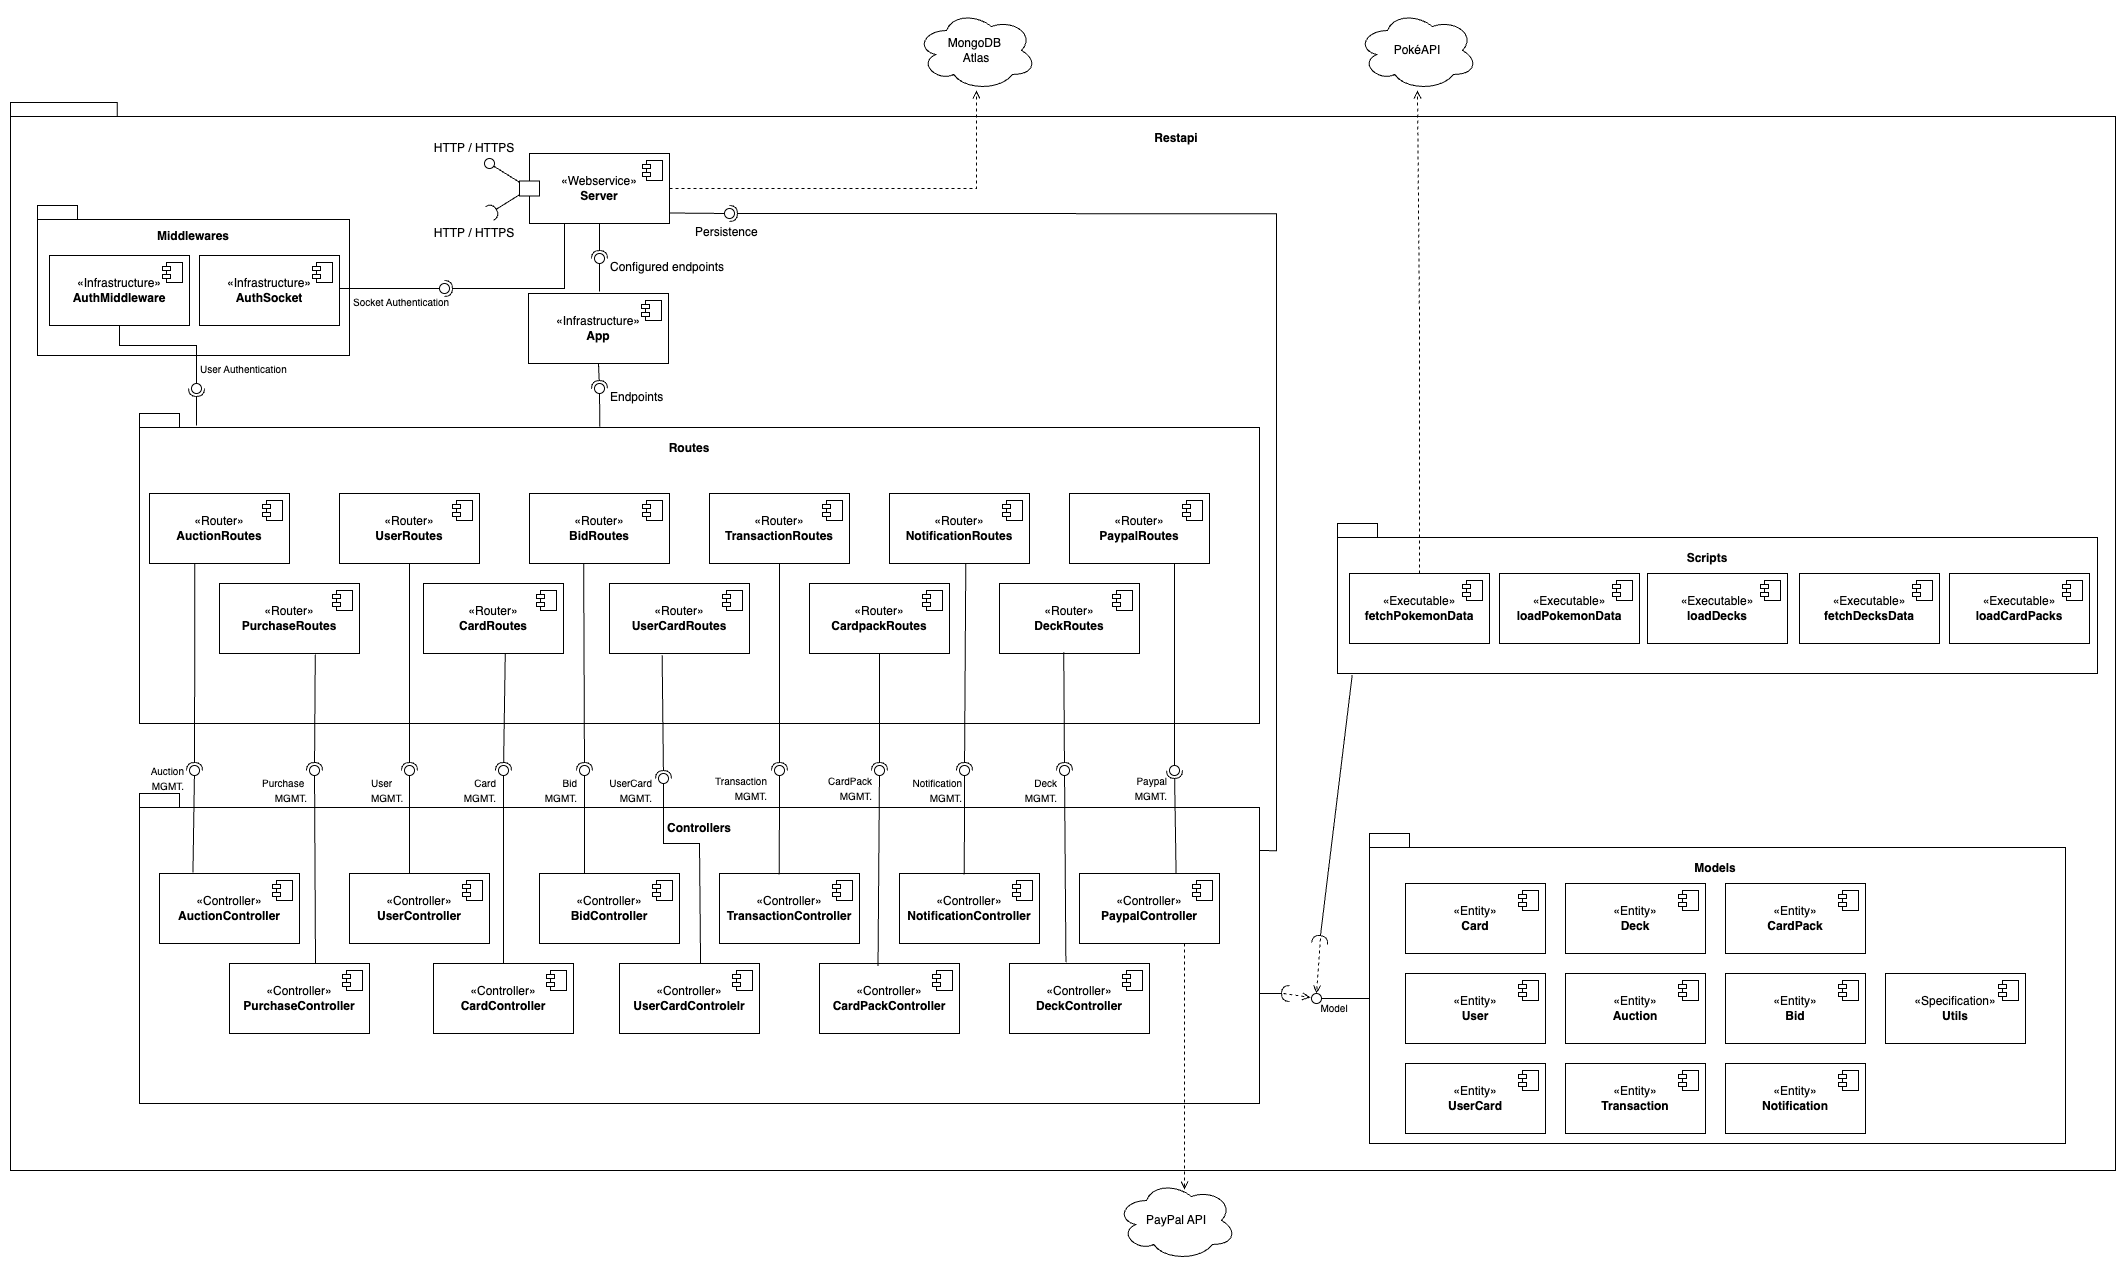
\includegraphics[width=1\linewidth]{figures/6-Analisis/6-Clases/6_5-Componentes-restapi.png}
        \caption{Diagrama de componentes del subsistema restapi}
        \label{fig:6_5_Diagrama-Componentes-restapi}
    \end{figure}
    \end{landscape}

\newpage

Por cada componente identificado en la \coloredUnderline{\hyperlink{fig:6_5_Diagrama-Componentes-restapi}{Figura \ref*{fig:6_5_Diagrama-Componentes-restapi}: \nameref*{fig:6_5_Diagrama-Componentes-restapi}}},
se ha creado una tabla con su descripción detallada, explicando su función específica dentro del sistema y las relaciones que mantiene con otros componentes.

\subsubsubsection{Descripción de componentes del subsistema restapi. \textit{Server} y \textit{App}}
%--- SERVER ---
\begin{longtable}{
    >{\columncolor{lightgreen!20}}p{4cm}
    p{12cm}
    }
    \caption{Descripción del componente:  Server} \label{table:descripcion_server} \\
    \toprule
    \rowcolor{darkgreen!50}
    \textbf{Componente} & \multicolumn{1}{>{\columncolor{darkgreen!50}\centering\arraybackslash}p{12cm}}{\textbf{SERVER}} \\
    \endfirsthead
    
    \multicolumn{2}{c}%
    {{ \tablename\ \thetable{} Descripción del componente:  Server -- continuación de la página anterior}} \\
    \toprule
    \rowcolor{darkgreen!50}
    \textbf{Componente} & \multicolumn{1}{>{\columncolor{darkgreen!50}\centering\arraybackslash}p{12cm}}{\textbf{SERVER}} \\
    \midrule
    \endhead
    
    \midrule
    \multicolumn{2}{r}{{Continúa en la siguiente página...}} \\ 
    \endfoot
    
    \bottomrule
    \endlastfoot
    
    \midrule
    Descripción & Este componente configura y gestiona los servidores HTTP y HTTPS, la conexión a MongoDB, y la gestión de conexiones de sockets mediante Socket.IO. También incluye la configuración de variables de entorno y el manejo de errores. \\
    \midrule
    Métodos & \begin{itemize}[nosep,leftmargin=*]
      \item \textbf{config()}: void, configura las variables de entorno.
      \item \textbf{createServers()}: void, crea y configura los servidores HTTP y HTTPS.
      \item \textbf{connectToDatabase()}: void, conecta a la base de datos MongoDB.
      \item \textbf{startServers()}: void, inicia los servidores HTTP y HTTPS.
      \item \textbf{setupSocketIO()}: void, configura el middleware de autenticación de sockets y maneja eventos de conexión y desconexión.
      \item \textbf{closeServer()}: Promise<void>, cierra los servidores HTTP, HTTPS y la conexión a la base de datos.
    \end{itemize} \\
    \midrule
    Interfaces requeridas & \begin{itemize}[nosep,leftmargin=*]
      \item \textbf{App}: Usa el componente App, que configura las rutas de la API REST.
      \item \textbf{AuthSocket}: Usa el middleware de autenticación de sockets.
      \item \textbf{HTTP/HTTPS}: Para la conexión a los servidores HTTP y HTTPS.
    \end{itemize} \\
    \midrule
    Interfaces proporcionadas & \begin{itemize}[nosep,leftmargin=*]
      \item \textbf{HTTP/HTTPS}: Proporciona la conexión a los servidores HTTP y HTTPS.
    \end{itemize} \\
\end{longtable}

%--- APP ---

\begin{longtable}{
    >{\columncolor{lightgreen!20}}p{4cm}
    p{12cm}
    }
    \caption{Descripción del componente:  App} \label{table:descripcion_app} \\
    \toprule
    \rowcolor{darkgreen!50}
    \textbf{Componente} & \multicolumn{1}{>{\columncolor{darkgreen!50}\centering\arraybackslash}p{12cm}}{\textbf{APP}} \\
    \endfirsthead
    
    \multicolumn{2}{c}%
    {{ \tablename\ \thetable{} Descripción del componente:  App -- continuación de la página anterior}} \\
    \toprule
    \rowcolor{darkgreen!50}
    \textbf{Componente} & \multicolumn{1}{>{\columncolor{darkgreen!50}\centering\arraybackslash}p{12cm}}{\textbf{APP}} \\
    \midrule
    \endhead
    
    \midrule
    \multicolumn{2}{r}{{Continúa en la siguiente página...}} \\ 
    \endfoot
    
    \bottomrule
    \endlastfoot
    
    \midrule
    Descripción & Este componente configura y gestiona las políticas CORS, las rutas de la API y el middleware para el manejo de errores. \\
    \midrule
    Métodos & \begin{itemize}[nosep,leftmargin=*]
      \item \textbf{use()}: void, permite configurar las rutas y los middlewares de la aplicación.
      \item \textbf{listen()}: void, inicia el servidor en el puerto especificado.
      \item \textbf{errorHandler()}: void, middleware para manejar errores en la aplicación.
    \end{itemize} \\
    \midrule
    Interfaces requeridas & \begin{itemize}[nosep,leftmargin=*]
      \item \textbf{Endpoints}: Utiliza todas las rutas de la API REST, definidas en el paquete \textit{routes}. Estas son:
        \begin{itemize}[nosep,leftmargin=*]
        \item \textbf{AuctionRouter}: Rutas que gestionan las subastas.
        \item \textbf{BidRouter}: Rutas que gestionan las pujas.
        \item \textbf{CardPackRouter}: Rutas que gestionan los sobres de cartas.
        \item \textbf{CardRouter}: Rutas que gestionan las cartas.
        \item \textbf{DeckRouter}: Rutas que gestionan los mazos de cartas.
        \item \textbf{NotificationRouter}: Rutas que gestionan las notificaciones.
        \item \textbf{PaypalRouter}: Rutas que gestionan las transacciones de PayPal.
        \item \textbf{PurchasesRouter}: Rutas que gestionan las compras.
        \item \textbf{TransactionRouter}: Rutas que gestionan las transacciones propias de la aplicación.
        \item \textbf{UserCardRouter}: Rutas que gestionan las cartas de usuario.
        \item \textbf{UserRouter}: Rutas que gestionan los usuarios.
        \end{itemize}
    \end{itemize} \\
    \midrule
    Interfaces proporcionadas & \begin{itemize}[nosep,leftmargin=*]
      \item \textbf{Configured endpoints}: Proporciona la aplicación de Express con las rutas y middlewares configurados.   
    \end{itemize} \\
\end{longtable}


%------------------------- PAQUETE MIDDLWARES -------------------------
\subsubsubsection{Descripción de componentes del subsistema restapi. Paquete \textit{middlewares}}\label{sec:descripcion_authmiddleware}
%--- AUTHMIDDLEWARE ---
\begin{longtable}{
    >{\columncolor{lightgreen!20}}p{4cm}
    p{12cm}
    }
    \caption{Descripción del componente:  AuthMiddleware} \label{table:descripcion_authmiddleware} \\
    \toprule
    \rowcolor{darkgreen!50}
    \textbf{Componente} & \multicolumn{1}{>{\columncolor{darkgreen!50}\centering\arraybackslash}p{12cm}}{\textbf{AUTHMIDDLEWARE}} \\
    \endfirsthead
    
    \multicolumn{2}{c}%
    {{ \tablename\ \thetable{} Descripción del componente:  AuthMiddleware -- continuación de la página anterior}} \\
    \toprule
    \rowcolor{darkgreen!50}
    \textbf{Componente} & \multicolumn{1}{>{\columncolor{darkgreen!50}\centering\arraybackslash}p{12cm}}{\textbf{AUTHMIDDLEWARE}} \\
    \midrule
    \endhead
    
    \midrule
    \multicolumn{2}{r}{{Continúa en la siguiente página...}} \\ 
    \endfoot
    
    \bottomrule
    \endlastfoot
    
    \midrule
    Descripción & Este componente proporciona middleware para la autenticación y autorización de usuarios mediante tokens JWT. Incluye la verificación de tokens y la verificación de roles de administrador. \\
    \midrule
    Métodos & \begin{itemize}[nosep,leftmargin=*]
      \item \textbf{auth(req: Request, res: Response, next: any)}: void, middleware para verificar la autenticidad del token JWT en las peticiones.
      \item \textbf{verifyAdmin(req: Request, res: Response, next: any)}: void, middleware para verificar que el usuario tiene rol de administrador.
    \end{itemize} \\
    \midrule
    Interfaces requeridas &  \\
    \midrule
    Interfaces proporcionadas & \begin{itemize}[nosep,leftmargin=*]
      \item \textbf{User Authentication}: Proporciona middleware para la autenticación de usuarios, verificando la validez del token JWT y, ofreciendo la posibilidad de verificar roles de administrador.
    \end{itemize} \\
    \end{longtable}

%--- AUTHSOCKET ---
\begin{longtable}{
    >{\columncolor{lightgreen!20}}p{4cm}
    p{12cm}
    }
    \caption{Descripción del componente:  AuthSocket} \label{table:descripcion_authsocket} \\
    \toprule
    \rowcolor{darkgreen!50}
    \textbf{Componente} & \multicolumn{1}{>{\columncolor{darkgreen!50}\centering\arraybackslash}p{12cm}}{\textbf{AUTHSOCKET}} \\
    \endfirsthead
    
    \multicolumn{2}{c}%
    {{ \tablename\ \thetable{} Descripción del componente:  AuthSocket -- continuación de la página anterior}} \\
    \toprule
    \rowcolor{darkgreen!50}
    \textbf{Componente} & \multicolumn{1}{>{\columncolor{darkgreen!50}\centering\arraybackslash}p{12cm}}{\textbf{AUTHSOCKET}} \\
    \midrule
    \endhead
    
    \midrule
    \multicolumn{2}{r}{{Continúa en la siguiente página...}} \\ 
    \endfoot
    
    \bottomrule
    \endlastfoot
    
    \midrule
    Descripción & Este componente proporciona el middleware para la autenticación de conexiones de sockets mediante tokens JWT. Verifica la validez y el formato del token proporcionado en el handshake de la conexión del socket. \\
    \midrule
    Métodos & \begin{itemize}[nosep,leftmargin=*]
      \item \textbf{authSocket(socket: Socket, next: (err?: Error) => void)}: void, middleware para verificar la autenticidad del token JWT en las conexiones de sockets.
    \end{itemize} \\
    \midrule
    Interfaces requeridas &  \\
    \midrule
    Interfaces proporcionadas & \begin{itemize}[nosep,leftmargin=*]
      \item \textbf{Socket Authentication}: Proporciona middleware para la autenticación de conexiones de sockets, verificando la validez del token JWT.
    \end{itemize} \\
    \end{longtable}

%------------------------- PAQUETE ROUTES -------------------------
\subsubsection{Descripción de componentes del subsistema restapi. Paquete \textit{routes}}
En el diagrama se muestra una relación de dependencia entre \textit{App} y los componentes del paquete \textit{routes}. 
En la práctica, cada componente del paquete \textit{routes} proporciona sus rutas a \textit{App} a través su propia instancia de \textit{Router} de Express. 
Se ha decidido simplificar la representación para facilitar la comprensión del diagrama, dado que todos los componentes del paquete \textit{routes} mantienen la misma relación con \textit{App}.

%--- AUCTIONROUTER ---
\begin{longtable}{
    >{\columncolor{lightgreen!20}}p{4cm}
    p{12cm}
    }
    \caption{Descripción del componente:  AuctionRouter} \label{table:descripcion_auctionrouter} \\
    \toprule
    \rowcolor{darkgreen!50}
    \textbf{Componente} & \multicolumn{1}{>{\columncolor{darkgreen!50}\centering\arraybackslash}p{12cm}}{\textbf{AUCTIONROUTER}} \\
    \endfirsthead
    
    \multicolumn{2}{c}%
    {{ \tablename\ \thetable{} Descripción del componente:  AuctionRouter -- continuación de la página anterior}} \\
    \toprule
    \rowcolor{darkgreen!50}
    \textbf{Componente} & \multicolumn{1}{>{\columncolor{darkgreen!50}\centering\arraybackslash}p{12cm}}{\textbf{AUCTIONROUTER}} \\
    \midrule
    \endhead
    
    \midrule
    \multicolumn{2}{r}{{Continúa en la siguiente página...}} \\ 
    \endfoot
    
    \bottomrule
    \endlastfoot
    
    \midrule
    Descripción & Este componente configura y gestiona las rutas relacionadas con las subastas en la aplicación Express. Incluye la autenticación mediante middleware y validaciones para las peticiones. \\
    \midrule
    Atributos & \begin{itemize}[nosep,leftmargin=*]
      \item \textbf{auctionRouter}: Router, instancia del enrutador de Express para las subastas.
    \end{itemize} \\
    \midrule
    Métodos & \begin{itemize}[nosep,leftmargin=*]
      \item \textbf{getAuctions(req: Request, res: Response)}: void, maneja la obtención de todas las subastas.
      \item \textbf{getAuction(req: Request, res: Response)}: void, maneja la obtención de una subasta por su ID.
      \item \textbf{getActiveAuctions(req: Request, res: Response)}: void, maneja la obtención de todas las subastas activas.
      \item \textbf{getActiveAuctionsByUser(req: Request, res: Response)}: void, maneja la obtención de todas las subastas activas de un usuario.
      \item \textbf{putUserCardUpForAuction(req: Request, res: Response)}: void, maneja la puesta en subasta de una carta de usuario.
      \item \textbf{withdrawnUserCardFromAuction(req: Request, res: Response)}: void, maneja la retirada de una carta de usuario de una subasta.
      \item \textbf{checkAllActiveAuctions(req: Request, res: Response)}: void, verifica todas las subastas activas y actualiza su estado si es necesario.
    \end{itemize} \\
    \midrule
    Interfaces requeridas &  \begin{itemize}[nosep,leftmargin=*]
      \item \textbf{User Authentication}: Middleware para la autenticación de usuarios.
      \item \textbf{Auction MGMT.}: Utiliza los métodos definidos en el controlador de subastas, \textit{AuctionController}.
    \end{itemize} \\
    \midrule
    Interfaces proporcionadas & \begin{itemize}[nosep,leftmargin=*]
      \item \textbf{Auction Router}: Proporciona las rutas para la gestión de subastas.
    \end{itemize} \\
    \end{longtable}

%--- BIDROUTER ---
\begin{longtable}{
    >{\columncolor{lightgreen!20}}p{4cm}
    p{12cm}
    }
    \caption{Descripción del componente:  BidRouter} \label{table:descripcion_bidrouter} \\
    \toprule
    \rowcolor{darkgreen!50}
    \textbf{Componente} & \multicolumn{1}{>{\columncolor{darkgreen!50}\centering\arraybackslash}p{12cm}}{\textbf{BIDROUTER}} \\
    \endfirsthead
    
    \multicolumn{2}{c}%
    {{ \tablename\ \thetable{} Descripción del componente:  BidRouter -- continuación de la página anterior}} \\
    \toprule
    \rowcolor{darkgreen!50}
    \textbf{Componente} & \multicolumn{1}{>{\columncolor{darkgreen!50}\centering\arraybackslash}p{12cm}}{\textbf{BIDROUTER}} \\
    \midrule
    \endhead
    
    \midrule
    \multicolumn{2}{r}{{Continúa en la siguiente página...}} \\ 
    \endfoot
    
    \bottomrule
    \endlastfoot
    
    \midrule
    Descripción & Este componente configura y gestiona las rutas relacionadas con las pujas en la aplicación Express. Incluye la autenticación mediante middleware y validaciones para las peticiones. \\
    \midrule
    Atributos & \begin{itemize}[nosep,leftmargin=*]
      \item \textbf{bidRouter}: Router, instancia del enrutador de Express para las pujas.
    \end{itemize} \\
    \midrule
    Métodos & \begin{itemize}[nosep,leftmargin=*]
      \item \textbf{getBidById(req: Request, res: Response)}: void, maneja la obtención de una puja por su ID.
      \item \textbf{createBid(req: Request, res: Response)}: void, maneja la creación de una nueva puja.
      \item \textbf{getActiveBidsByUser(req: Request, res: Response)}: void, maneja la obtención de todas las pujas activas de un usuario.
      \item \textbf{withdrawBid(req: Request, res: Response)}: void, maneja la retirada de una puja.
    \end{itemize} \\
    \midrule
    Relaciones & \begin{itemize}[nosep,leftmargin=*]
      \item \textbf{AuthMiddleware}: Middleware para la autenticación de usuarios.
      \item \textbf{BidController}: Importa y utiliza métodos del controlador de pujas.
    \end{itemize} \\
    \midrule
    Interfaces requeridas & \begin{itemize}[nosep,leftmargin=*]
      \item \textbf{User Authentication}: Middleware para la autenticación de usuarios.
      \item \textbf{Bid MGMT.}: Utiliza los métodos definidos en el controlador de pujas, \textit{BidController}.
    \end{itemize} \\
    \midrule
    Interfaces proporcionadas & \begin{itemize}[nosep,leftmargin=*]
      \item \textbf{Bid Router}: Proporciona las rutas para la gestión de pujas.
    \end{itemize} \\
    \end{longtable}

\subsubsubsection{Descripción del componente:  CardPackRouter} \label{sec:descripcion_cardpackrouter}
\begin{longtable}{
    >{\columncolor{lightgreen!20}}p{4cm}
    p{12cm}
    }
    \caption{Descripción del componente:  CardPackRouter} \label{table:descripcion_cardpackrouter} \\
    \toprule
    \rowcolor{darkgreen!50}
    \textbf{Componente} & \multicolumn{1}{>{\columncolor{darkgreen!50}\centering\arraybackslash}p{12cm}}{\textbf{CARDPACKROUTER}} \\
    \endfirsthead
    
    \multicolumn{2}{c}%
    {{ \tablename\ \thetable{} Descripción del componente:  CardPackRouter -- continuación de la página anterior}} \\
    \toprule
    \rowcolor{darkgreen!50}
    \textbf{Componente} & \multicolumn{1}{>{\columncolor{darkgreen!50}\centering\arraybackslash}p{12cm}}{\textbf{CARDPACKROUTER}} \\
    \midrule
    \endhead
    
    \midrule
    \multicolumn{2}{r}{{Continúa en la siguiente página...}} \\ 
    \endfoot
    
    \bottomrule
    \endlastfoot
    
    \midrule
    Descripción & Este componente configura y gestiona las rutas relacionadas con los sobres de cartas en la aplicación Express. Incluye la autenticación mediante middleware. \\
    \midrule
    Métodos & \begin{itemize}[nosep,leftmargin=*]
      \item \textbf{getCardPacks(req: Request, res: Response)}: void, maneja la obtención de todos los sobres de cartas.
    \end{itemize} \\
    \midrule
    Interfaces requeridas & \begin{itemize}[nosep,leftmargin=*]
      \item \textbf{User Authentication}: Middleware para la autenticación de usuarios.
      \item \textbf{CardPack MGMT.}: Utiliza los métodos definidos en el controlador de sobres de cartas, \textit{CardPackController}.
    \end{itemize} \\
    \midrule
    Interfaces proporcionadas & \begin{itemize}[nosep,leftmargin=*]
      \item \textbf{CardPack Router}: Proporciona las rutas para la gestión de sobres de cartas.
    \end{itemize} \\
    \end{longtable}


%--- CARDROUTER ---
\begin{longtable}{
    >{\columncolor{lightgreen!20}}p{4cm}
    p{12cm}
    }
    \caption{Descripción del componente:  CardRouter} \label{table:descripcion_cardrouter} \\
    \toprule
    \rowcolor{darkgreen!50}
    \textbf{Componente} & \multicolumn{1}{>{\columncolor{darkgreen!50}\centering\arraybackslash}p{12cm}}{\textbf{CARDROUTER}} \\
    \endfirsthead
    
    \multicolumn{2}{c}%
    {{ \tablename\ \thetable{} Descripción del componente:  CardRouter -- continuación de la página anterior}} \\
    \toprule
    \rowcolor{darkgreen!50}
    \textbf{Componente} & \multicolumn{1}{>{\columncolor{darkgreen!50}\centering\arraybackslash}p{12cm}}{\textbf{CARDROUTER}} \\
    \midrule
    \endhead
    
    \midrule
    \multicolumn{2}{r}{{Continúa en la siguiente página...}} \\ 
    \endfoot
    
    \bottomrule
    \endlastfoot
    
    \midrule
    Descripción & Esta clase configura y gestiona las rutas relacionadas con las cartas en la aplicación Express. Incluye la autenticación mediante middleware y validaciones para las peticiones. \\
    \midrule
    Métodos & \begin{itemize}[nosep,leftmargin=*]
      \item \textbf{getCard(req: Request, res: Response)}: void, maneja la obtención de una carta por su ID.
    \end{itemize} \\
    \midrule
    Interfaces requeridas  & \begin{itemize}[nosep,leftmargin=*]
      \item \textbf{User Authentication}: Middleware para la autenticación de usuarios.
      \item \textbf{Card MGMT.}: Utiliza los métodos definidos en el controlador de cartas, \textit{CardController}.
    \end{itemize} \\
    \midrule
    Interfaces proporcionadas & \begin{itemize}[nosep,leftmargin=*]
        \item \textbf{Card Router}: Proporciona las rutas para la gestión de cartas.
    \end{itemize} \\
    \end{longtable}

% --- NOTIFICATIONROUTER ---
\begin{longtable}{
    >{\columncolor{lightgreen!20}}p{4cm}
    p{12cm}
    }
    \caption{Descripción del componente:  NotificationRouter} \label{table:descripcion_notificationrouter} \\
    \toprule
    \rowcolor{darkgreen!50}
    \textbf{Componente} & \multicolumn{1}{>{\columncolor{darkgreen!50}\centering\arraybackslash}p{12cm}}{\textbf{NOTIFICATIONROUTER}} \\
    \endfirsthead
    
    \multicolumn{2}{c}%
    {{ \tablename\ \thetable{} Descripción del componente:  NotificationRouter -- continuación de la página anterior}} \\
    \toprule
    \rowcolor{darkgreen!50}
    \textbf{Componente} & \multicolumn{1}{>{\columncolor{darkgreen!50}\centering\arraybackslash}p{12cm}}{\textbf{NOTIFICATIONROUTER}} \\
    \midrule
    \endhead
    
    \midrule
    \multicolumn{2}{r}{{Continúa en la siguiente página...}} \\ 
    \endfoot
    
    \bottomrule
    \endlastfoot
    
    \midrule
    Descripción & Este componente configura y gestiona las rutas relacionadas con las notificaciones en la aplicación Express. Incluye la autenticación mediante middleware y validaciones para las peticiones. \\
    \midrule
    Atributos & \begin{itemize}[nosep,leftmargin=*]
      \item \textbf{notificationRouter}: Router, instancia del enrutador de Express para las notificaciones.
    \end{itemize} \\
    \midrule
    Métodos & \begin{itemize}[nosep,leftmargin=*]
      \item \textbf{getNotifications(req: Request, res: Response)}: void, maneja la obtención de todas las notificaciones de un usuario.
      \item \textbf{markAsRead(req: Request, res: Response)}: void, maneja el marcado de una notificación como leída.
      \item \textbf{markAllAsRead(req: Request, res: Response)}: void, maneja el marcado de todas las notificaciones de un usuario como leídas.
      \item \textbf{hasUnreadNotifications(req: Request, res: Response)}: void, verifica si un usuario tiene notificaciones no leídas.
    \end{itemize} \\
    \midrule
    Interfaces requeridas & \begin{itemize}[nosep,leftmargin=*]
      \item \textbf{User Authentication}: Middleware para la autenticación de usuarios.
      \item \textbf{Notification MGMT.}: Utiliza los métodos definidos en el controlador de notificaciones, \textit{NotificationController}.
    \end{itemize} \\
    \midrule
    Interfaces proporcionadas & \begin{itemize}[nosep,leftmargin=*]
        \item \textbf{Notification Router}: Proporciona las rutas para la gestión de notificaciones.
    \end{itemize} \\
    \end{longtable}

%--- PAYPALROUTER ---
\begin{longtable}{
    >{\columncolor{lightgreen!20}}p{4cm}
    p{12cm}
    }
    \caption{Descripción del componente:  PaypalRouter} \label{table:descripcion_paypalrouter} \\
    \toprule
    \rowcolor{darkgreen!50}
    \textbf{Componente} & \multicolumn{1}{>{\columncolor{darkgreen!50}\centering\arraybackslash}p{12cm}}{\textbf{PAYPALROUTER}} \\
    \endfirsthead
    
    \multicolumn{2}{c}%
    {{ \tablename\ \thetable{} Descripción del componente:  PaypalRouter -- continuación de la página anterior}} \\
    \toprule
    \rowcolor{darkgreen!50}
    \textbf{Componente} & \multicolumn{1}{>{\columncolor{darkgreen!50}\centering\arraybackslash}p{12cm}}{\textbf{PAYPALROUTER}} \\
    \midrule
    \endhead
    
    \midrule
    \multicolumn{2}{r}{{Continúa en la siguiente página...}} \\ 
    \endfoot
    
    \bottomrule
    \endlastfoot
    
    \midrule
    Descripción & Este componente configura y gestiona las rutas relacionadas con las órdenes de PayPal en la aplicación Express. Incluye validaciones para las peticiones y manejo de errores. \\
    \midrule
    Métodos & \begin{itemize}[nosep,leftmargin=*]
      \item \textbf{createOrder(req: Request, res: Response)}: void, maneja la creación de una nueva orden de PayPal.
      \item \textbf{updateOrder(req: Request, res: Response)}: void, maneja la actualización del saldo de un usuario después de completar un pago.
    \end{itemize} \\
    \midrule
    Interfaces requeridas & \begin{itemize}[nosep,leftmargin=*]
      \item \textbf{Paypal MGMT.}: Utiliza los métodos definidos en el controlador de PayPal, \textit{PaypalController}.
    \end{itemize} \\
    \midrule
    Interfaces proporcionadas & \begin{itemize}[nosep,leftmargin=*]
      \item \textbf{Paypal Router}: Proporciona las rutas para la gestión de órdenes de PayPal.
    \end{itemize} \\
    \end{longtable}

%------------------------- PAQUETE CONTROLLERS -------------------------



\subsubsection{Diagrama de componentes del subsistema webapp}
A continuación, se presenta el diagrama de componentes del subsistema \textbf{webapp}. En este diagrama se muestran los componentes que forman parte del subsistema.
Se han omitido las relaciones entre los componentes para simplificar el diagrama. Las relaciones entre los componentes se explicarán en la descripción de los componentes.
\begin{landscape}
    \begin{figure}[H]
        \hypertarget{fig:6_5_Diagrama-Componentes-webapp}{}
        \centering
        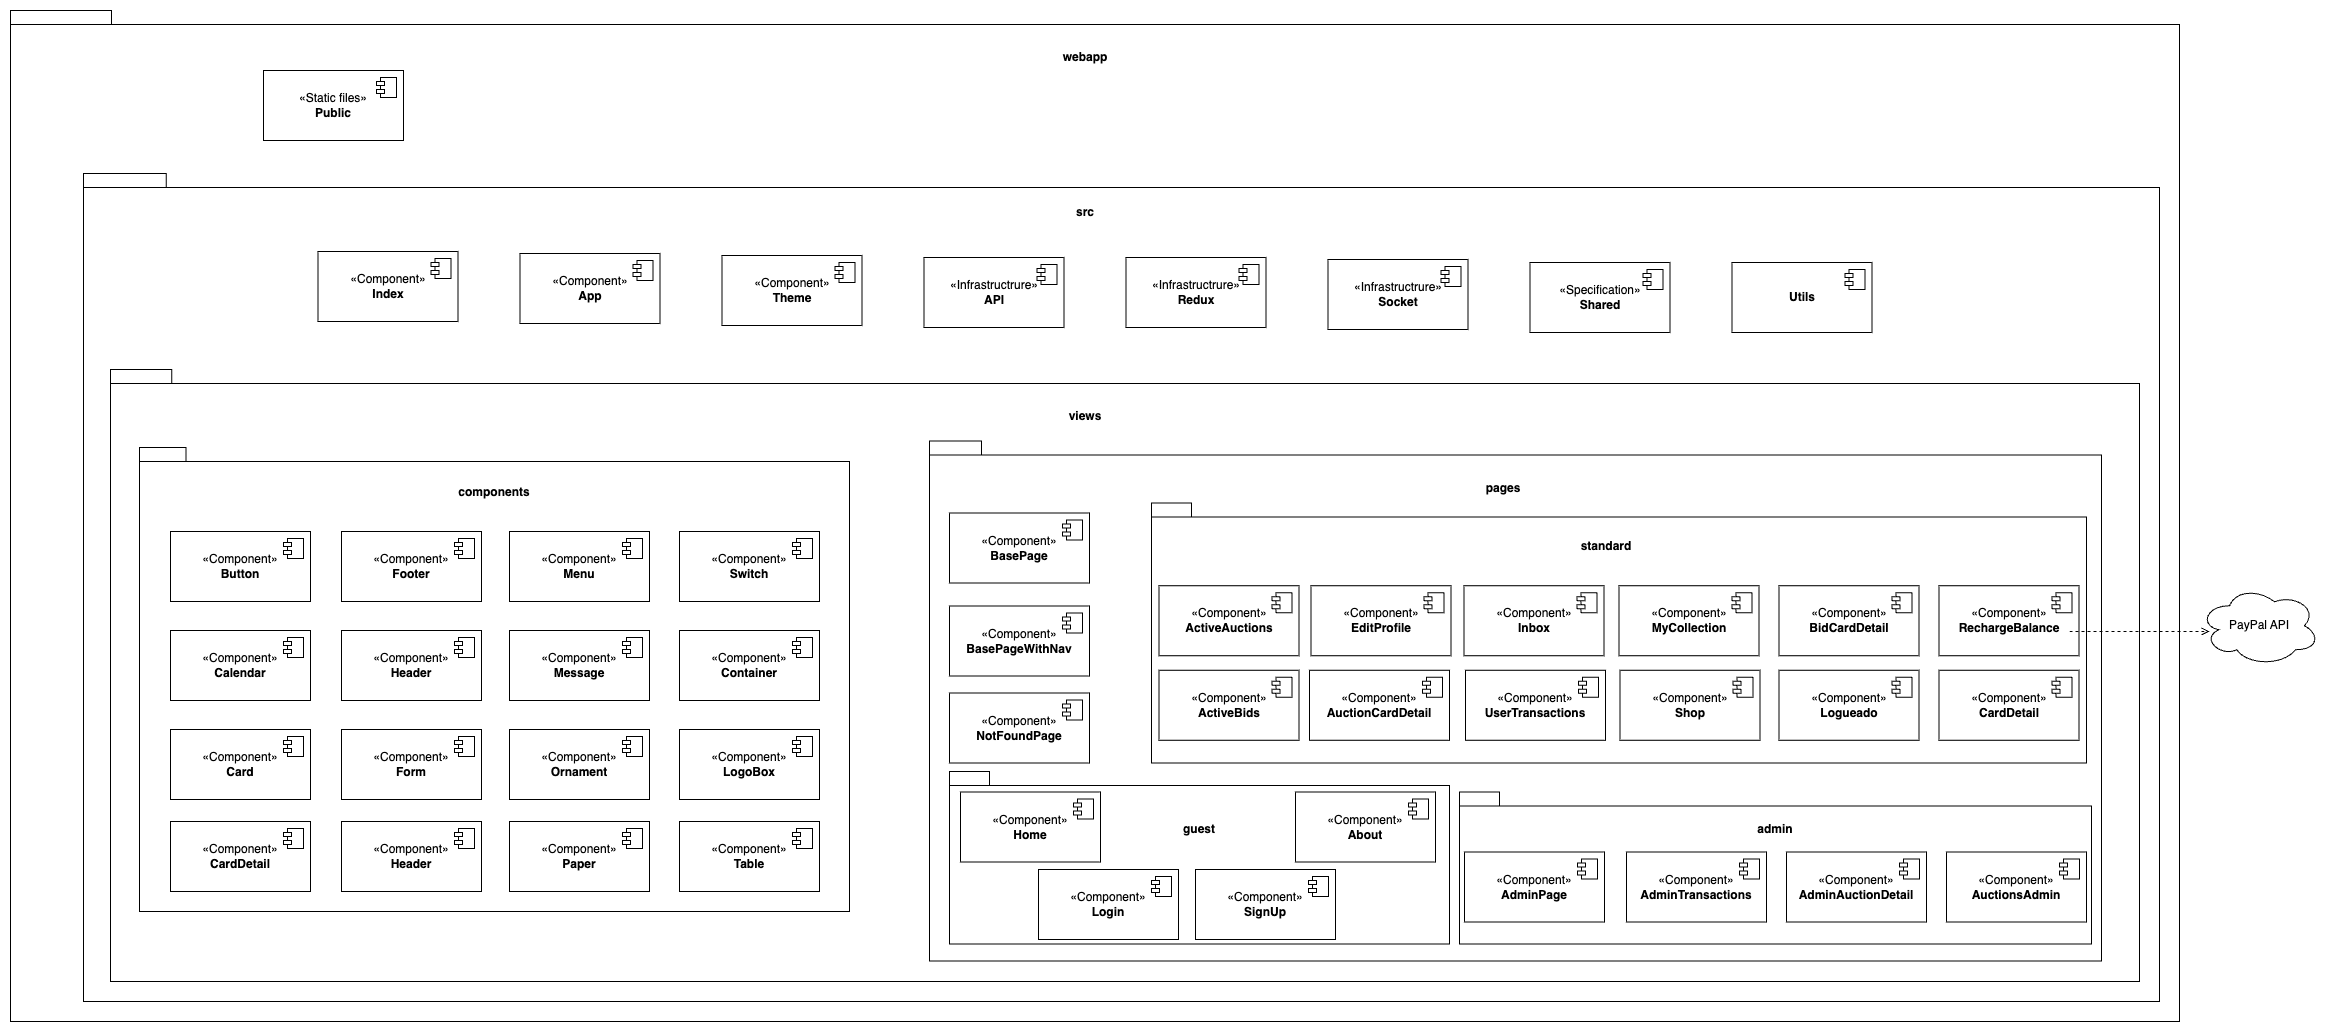
\includegraphics[width=1\linewidth]{figures/6-Analisis/6-Clases/6_5-Componentes-webapp.png}
        \caption{Diagrama de componentes del subsistema webapp}
        \label{fig:6_5_Diagrama-Componentes-webapp}
    \end{figure}
    \end{landscape}

\newpage

\subsubsubsection{Descripción de los Componentes del Subsistema webapp}
En este apartado se describirá la funcionalidad de los componentes del subsistema webapp. 
\begin{itemize}
    \item \textbf{Index}: Es el punto de entrada de la aplicación. Este componente se encarga del renderizado del componente \textit{App}.
    \item \textbf{App}: es el componente principal de la aplicación. Este componente define el diagrama de navegabilidad de la aplicación y se encarga de renderizar los componentes de la aplicación en función de la ruta actual. 
    Se relaciona, por lo tanto, con el paquete \textit{pages} y con el componente \textit{Theme} para definir el tema de la aplicación.
    \item \textbf{Theme}: es el componente que define el tema de la aplicación. Este componente se encarga de definir los colores y tipografías de la aplicación.
    \item \textbf{API}: es el componente que se encarga de realizar las peticiones a la API. Este componente se relaciona con el paquete \textit{shared} para definir los tipos de datos compartidos entre las distintas partes de la aplicación.
    \item \textbf{Redux}: es el componente que se encarga de gestionar el estado de la aplicación. Gestiona los siguientes estados:
    \begin{itemize}
        \item \textbf{user}: contiene la información del usuario autenticado.
        \item \textbf{notification}: estado para gestionar las visualizaciones de las notificaciones en tiempo real.
        \item \textbf{update}: estado para gestionar las actualizaciones de los datos de la aplicación.
    \end{itemize}
    \item \textbf{Socket}: es el componente que se encarga de gestionar la conexión con Socket.io. Concretamente se utiliza para que los usuarios puedan recibir notificaciones en tiempo real.
    \item \textbf{Shared}: es el componente que se encarga de definir los tipos de datos compartidos entre las distintas partes de la aplicación.
    \item \textbf{Utils}: es el componente que se encarga de definir utilidades de la aplicación. Contiene las siguientes utilidades:
    \begin{itemize}
        \item \textbf{cardData}: Colección de cartas de ejemplo para la aplicación. Se utiliza en un componente de la aplicación para mostrar cartas de ejemplo.
        \item \textbf{fieldsValidation}: utilidad para validar los campos de un formulario.
        \item \textbf{PrivateRoute}: componente que implementa una ruta privada de la aplicación. Verifica que un usuario esté autenticado antes de renderizar un componente.
        \item \textbf{RouteRedirector}: componente que implementa un redireccionador de rutas de la aplicación. Redirige a la ruta solicitada si el usuario cumple con el rol requerido, en caso contrario redirige a la ruta por defecto.
        \item \textbf{utils}: funciones de utilidad para la aplicación, como conversión de fechas y generación de mensajes.
    \end{itemize}
    \item \textbf{views}: contiene los componentes que implementan las vistas de la aplicación, y se divide en los siguientes subpaquetes:
    \begin{itemize}
        \item \textbf{components}: contiene los archivos que implementan los componentes de la aplicación. 
        Estos se usan para definir componentes más complejos que se reutilizan en distintas partes de la aplicación.
        \begin{itemize}
            \item \textbf{Button}: componente que implementa un botón de la aplicación. En este componente se definen los distintos tipos de botones que se utilizan en la aplicación.
            \item \textbf{Calendar}: componente que implementa un calendario de la aplicación.
            \item \textbf{Card}: componente que implementa una carta de la aplicación. 
            \item \textbf{CardDetail}: componente que implementa el modelo base de un detalle de carta.
            \item \textbf{Cardpack}: componente que implementa un sobre de cartas de la aplicación.
            \item \textbf{Container}: componente que implementa distintos tipos de contenedores de la aplicación.
            \item \textbf{Form}: componente que define los formularios de la aplicación.
            \item \textbf{Footer}: componente que implementa el pie de página de la aplicación.
            \item \textbf{Header}: componente que implementa la cabecera de la aplicación.
            \item \textbf{LogoBox}: componente que implementa el logotipo de la aplicación.
            \item \textbf{Menu}: componente que implementa los distintos menús de la aplicación.
            \item \textbf{Messages}: componente que implementa los distintos mensajes informativos de la aplicación.
            \item \textbf{Ornament}: componente que implementa distintos adornos de la aplicación.
            \item \textbf{Paper}: componente que implementa un contenedor con sombra, se utiliza para mostrar información en la aplicación.
            \item \textbf{Switch}: componente que implementa un interruptor de la aplicación. Concretamente, se utiliza para cambiar entre los modos claro y oscuro de la temática de la aplicación.
            \item \textbf{Table}: componente que implementa una tabla de la aplicación.
        \end{itemize}
        \item \textbf{pages}: contiene los archivos que implementan las páginas de la aplicación. Las páginas definen la estructura de las distintas vistas de la aplicación.
        Estas se crean utilizando los componentes definidos en el paquete \textit{components} junto con otros componentes de React.
        \begin{itemize}
            \item \textbf{BasePage}: página que implementa la estructura base de una página de la aplicación.
            \item \textbf{BasePageWithNav}: página que implementa la estructura base de una página de la aplicación con navegación.
            \item \textbf{NotFoundPage}: página que implementa la página de error 404.
            \item En el paquete \textit{guest} se encuentran las páginas que puede ver cualquier usuario:
            \begin{itemize}
                \item \textbf{Home}: página principal de la aplicación.
                \item \textbf{Login}: página de inicio de sesión.
                \item \textbf{SignUp}: página de registro de usuario.
                \item \textbf{About}: página de información sobre la aplicación.
            \end{itemize}
             \item En el paquete \textit{admin} se encuentran las páginas que puede ver un usuario con rol de administrador:
            \begin{itemize}
                \item \textbf{AdminPage}: página de administración de la aplicación.
                \item \textbf{AdminTransactions}: página de administración de usuarios.
                \item \textbf{AdminAuctionDetail}: página de administración de transacciones.
                \item \textbf{AuctionsAdmin}: página de administración de subastas.
            \end{itemize}
            \item En el paquete \textit{standard} se encuentran las páginas que puede ver un usuario autenticado con rol de usuario no administrador:
            \begin{itemize}
                \item \textbf{Logueado}: página de inicio del usuario autenticado.
                \item \textbf{EditProfile}: página de perfil del usuario autenticado.
                \item \textbf{CardDetail}: página de detalle de carta.
                \item \textbf{AuctionCardDetail}: página que muestra el detalle de una carta en subasta.
                \item \textbf{BidCardDetail}: página que muestra el detalle de una puja realizada a una determinada carta.
                \item \textbf{Shop}: página de tienda, en ella el usuario puede adquirir sobres de cartas.
                \item \textbf{ActiveAuctions}: página de subastas, en ella el usuario puede participar en subastas.
                \item \textbf{UserTransactions}: página de transacciones, en ella el usuario puede consultar las subastas realizadas.
                \item \textbf{InBox}: página de notificaciones, en ella el usuario puede consultar las notificaciones recibidas.
                \item \textbf{MyCollection}: página de colección, en ella el usuario puede consultar las cartas que posee.
                \item \textbf{RechargeBalance}: página de recarga de saldo, en ella el usuario puede recargar su saldo. Se comunica por HTTPS con la pasarela de pago, en este caso con la API de PayPal.
            \end{itemize}
        \end{itemize}
    \end{itemize}
\end{itemize}

% Nota adicional sobre los componentes
\bigskip
\textbf{Nota:} En el diagrama de componentes, una caja no necesariamente representa un único componente; puede representar múltiples componentes. 
Por ejemplo, en el caso del componente \textit{Button}, en la práctica se han implementado varios componentes que representan distintos tipos de botones de la aplicación.


\subsection{Diagrama de Despliegue}
En este apartado se describirá el proceso de despliegue de la aplicación, detallando los componentes y servicios necesarios para su correcto funcionamiento. 
Se presentará un diagrama de despliegue que ilustrará la arquitectura de la aplicación y la distribución de los componentes en el entorno de ejecución. 

Como se ha visto en la sección \coloredUnderline{\hyperlink{sec:identificacion-subsistemas-analisis}{\ref*{sec:identificacion-subsistemas-analisis}. \nameref*{sec:identificacion-subsistemas-analisis}}}, la aplicación se divide en dos subsistemas principales: \textbf{restapi} y \textbf{webapp}.
El subsistema \textbf{restapi} contiene las clases que implementan la API REST y la lógica de negocio, mientras que el subsistema \textbf{webapp} abarca la interfaz de usuario de la aplicación.
Estos dos subsistemas serán desplegados en una máquina virtual de Azure, utilizando contenedores Docker para facilitar su despliegue y escalabilidad.

Para desplegar la aplicación, se han seguido los siguientes pasos:
\begin{enumerate}
    \item \textbf{Crear la máquina virtual en Azure}: Se ha creado una máquina virtual en Azure con las características mencionadas anteriormente. 
    Además, es necesario crear un grupo de recursos y una red virtual para la máquina virtual. Las características de la máquina virtual son las siguientes:
    \begin{itemize}
        \item \textbf{Sistema Operativo}: Ubuntu 20.04 LTS.
        \item \textbf{Procesador}: 2 núcleos.
        \item \textbf{Memoria RAM}: 4 GB.
        \item \textbf{Discos de datos}: 4.
        \item \textbf{E/S máxima}: 1280 MB/s.
        \item \textbf{Almacenamiento local}: 8 GB.
        \item \textbf{Red}: IP pública y DNS asociado.
    \end{itemize}

    \item \textbf{Establecer un nombre de dominio}: Se ha asociado un nombre de dominio a la dirección IP pública de la máquina virtual para facilitar el acceso a la aplicación.

    \item \textbf{Contenedores Docker}: Se ha utilizado Docker para contenerizar la aplicación y facilitar su despliegue. 
    Para facilitar la tarea se ha configurado integración continua con GitHub Actions, de forma que cada vez que se realiza un \textit{pull-request} a la rama principal del repositorio, se construyen y despliegan los contenedores en la máquina virtual de Azure.
    Se han creado dos contenedores, uno para el subsistema \textbf{restapi} y otro para el subsistema \textbf{webapp}. Cada uno de estos expone uno o varios puertos diferentes para la comunicación con el exterior.

    \item \textbf{Configuración de Nginx como Proxy Inverso}: Se ha configurado Nginx como servidor web inverso para redirigir las peticiones a los contenedores correspondientes.
    Este paso es necesario para poder garantizar la seguridad de las comunicaciones con HTTPS. La configuración de Nginx incluye:
    \begin{itemize}
        \item \textbf{Obtención de certificado SSL}: Se ha utilizado Certbot para obtener un certificado SSL gratuito de Let's Encrypt y habilitar el protocolo HTTPS en la aplicación.
        \item \textbf{Redirección de Peticiones}: Configuración de Nginx para dirigir el tráfico HTTP y HTTPS a los contenedores adecuados.
    \end{itemize}

    \item \textbf{Configuración de la base de datos}: En la aplicación se usa como base de datos Mongo DB Atlas, que es una base de datos en la nube por lo que no es necesario configurarla en la máquina virtual, 
    pero sí es necesario configurar la conexión a la base de datos en la aplicación y permitir el acceso desde la dirección IP de la máquina virtual.

    \item \textbf{Docker Compose}: Se ha utilizado Docker Compose para orquestar los contenedores de la aplicación y facilitar su despliegue en la máquina virtual de Azure.
    Se ha creado un archivo \textit{docker-compose.yml} en la máquina virtual que define los servicios de la aplicación y sus configuraciones.

\end{enumerate}

Una vez realizados estos pasos, la aplicación estará desplegada y accesible a través del nombre de dominio asociado a la dirección IP pública de la máquina virtual.
Debido a los costos asociados al uso de la máquina virtual en Azure, se ha optado por mantener la máquina virtual apagada cuando no se está utilizando la aplicación.


En la \coloredUnderline{\hyperlink{fig:6_6_Diagrama-Despliegue}{Figura \ref*{fig:6_6_Diagrama-Despliegue}: \nameref*{fig:6_6_Diagrama-Despliegue}}} se muestra el diagrama de despliegue de la aplicación.
\begin{figure}[H]
    \hypertarget{fig:6_6_Diagrama-Despliegue}{}
    \centering
    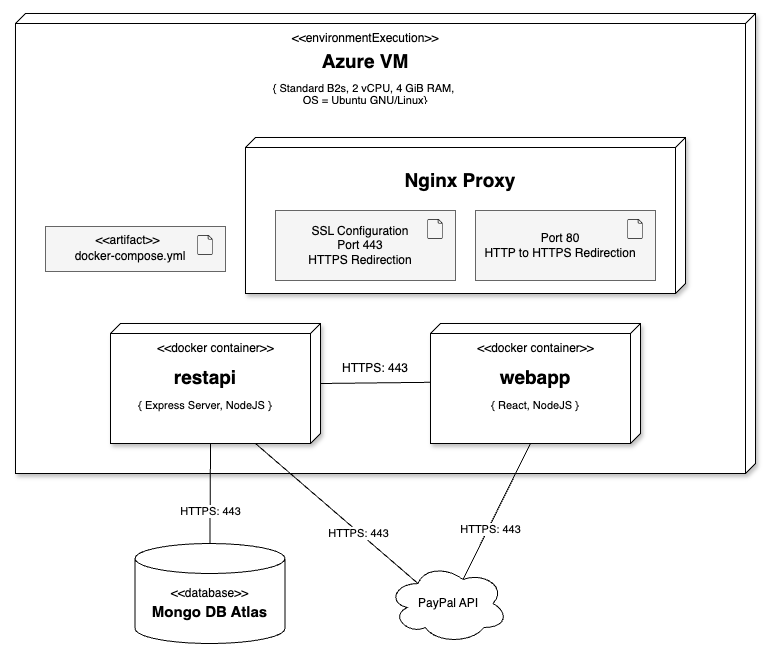
\includegraphics[width=0.8\linewidth]{figures/6-Analisis/6-Clases/6_5-Deployment.png}
    \caption{Diagrama de Despliegue de la Aplicación}
    \label{fig:6_6_Diagrama-Despliegue}
\end{figure}


\newpage
\section{DEFINICIÓN DE INTERFACES DE USUARIO}
\subsection{Descripción de la Interfaz} 
Se ha desarrollado un conjunto de bocetos representativos para cada una de las interfaces principales, con el objetivo de facilitar la comprensión visual y estructural del sistema. 
Se ha decidido omitir la creación de bocetos para ciertas páginas del sistema, considerando que su simplicidad inherente no justifica una representación gráfica detallada, 
o debido a que su diseño es análogo al de otras interfaces previamente especificadas. 

\subsubsection{Página de Inicio}
La página de inicio es la primera página que se muestra al usuario al acceder al sistema.
Esta página se muestra cuando el usuario no ha iniciado sesión, y le permite acceder a las siguientes funcionalidades:
\begin{itemize}
    \item Iniciar sesión.
    \item Registrarse.
    \item Consultar información pública sobre el sistema (Enlaces del pie de página)
\end{itemize}

En la figura \ref{fig:p_home} se muestra el boceto de la página de inicio.

\begin{figure}[H]
    \centering
    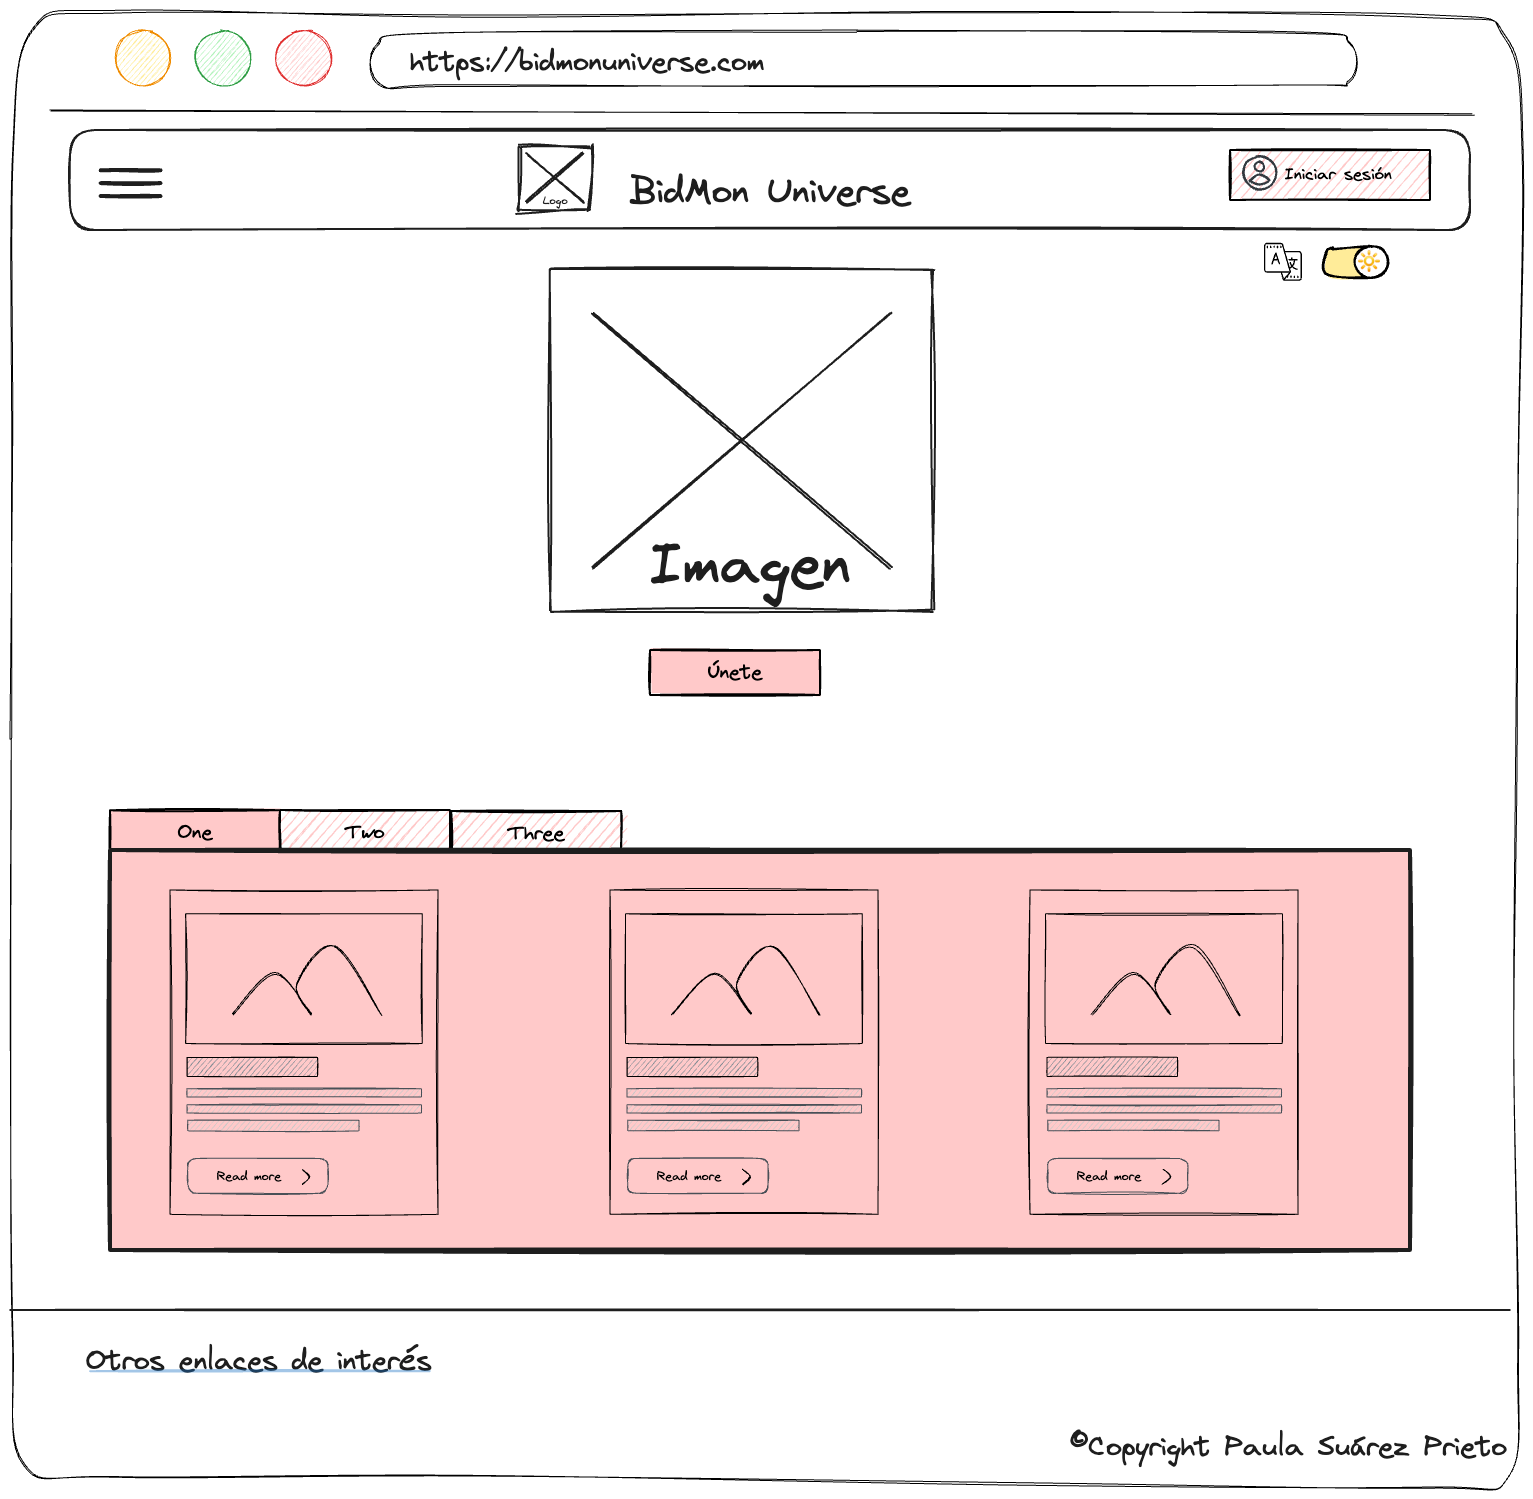
\includegraphics[width=0.8\textwidth]{figures/6-Analisis/6-Interfaz/prototipos/home.png}
    \caption{Boceto de la página de inicio}
    \label{fig:p_home}
\end{figure}

\subsubsection{Página de Inicio de Sesión}
La página de inicio de sesión muestra un formulario que permite al usuario ingresar sus credenciales para acceder al sistema o recuperar su contraseña.
En la figura \ref{fig:p_login} se muestra el boceto de la página de inicio de sesión.
En caso de que el usuario introduzca credenciales incorrectas, se mostrará un mensaje de error y se resaltarán los campos correspondientes.

\begin{figure}[H]
    \centering
    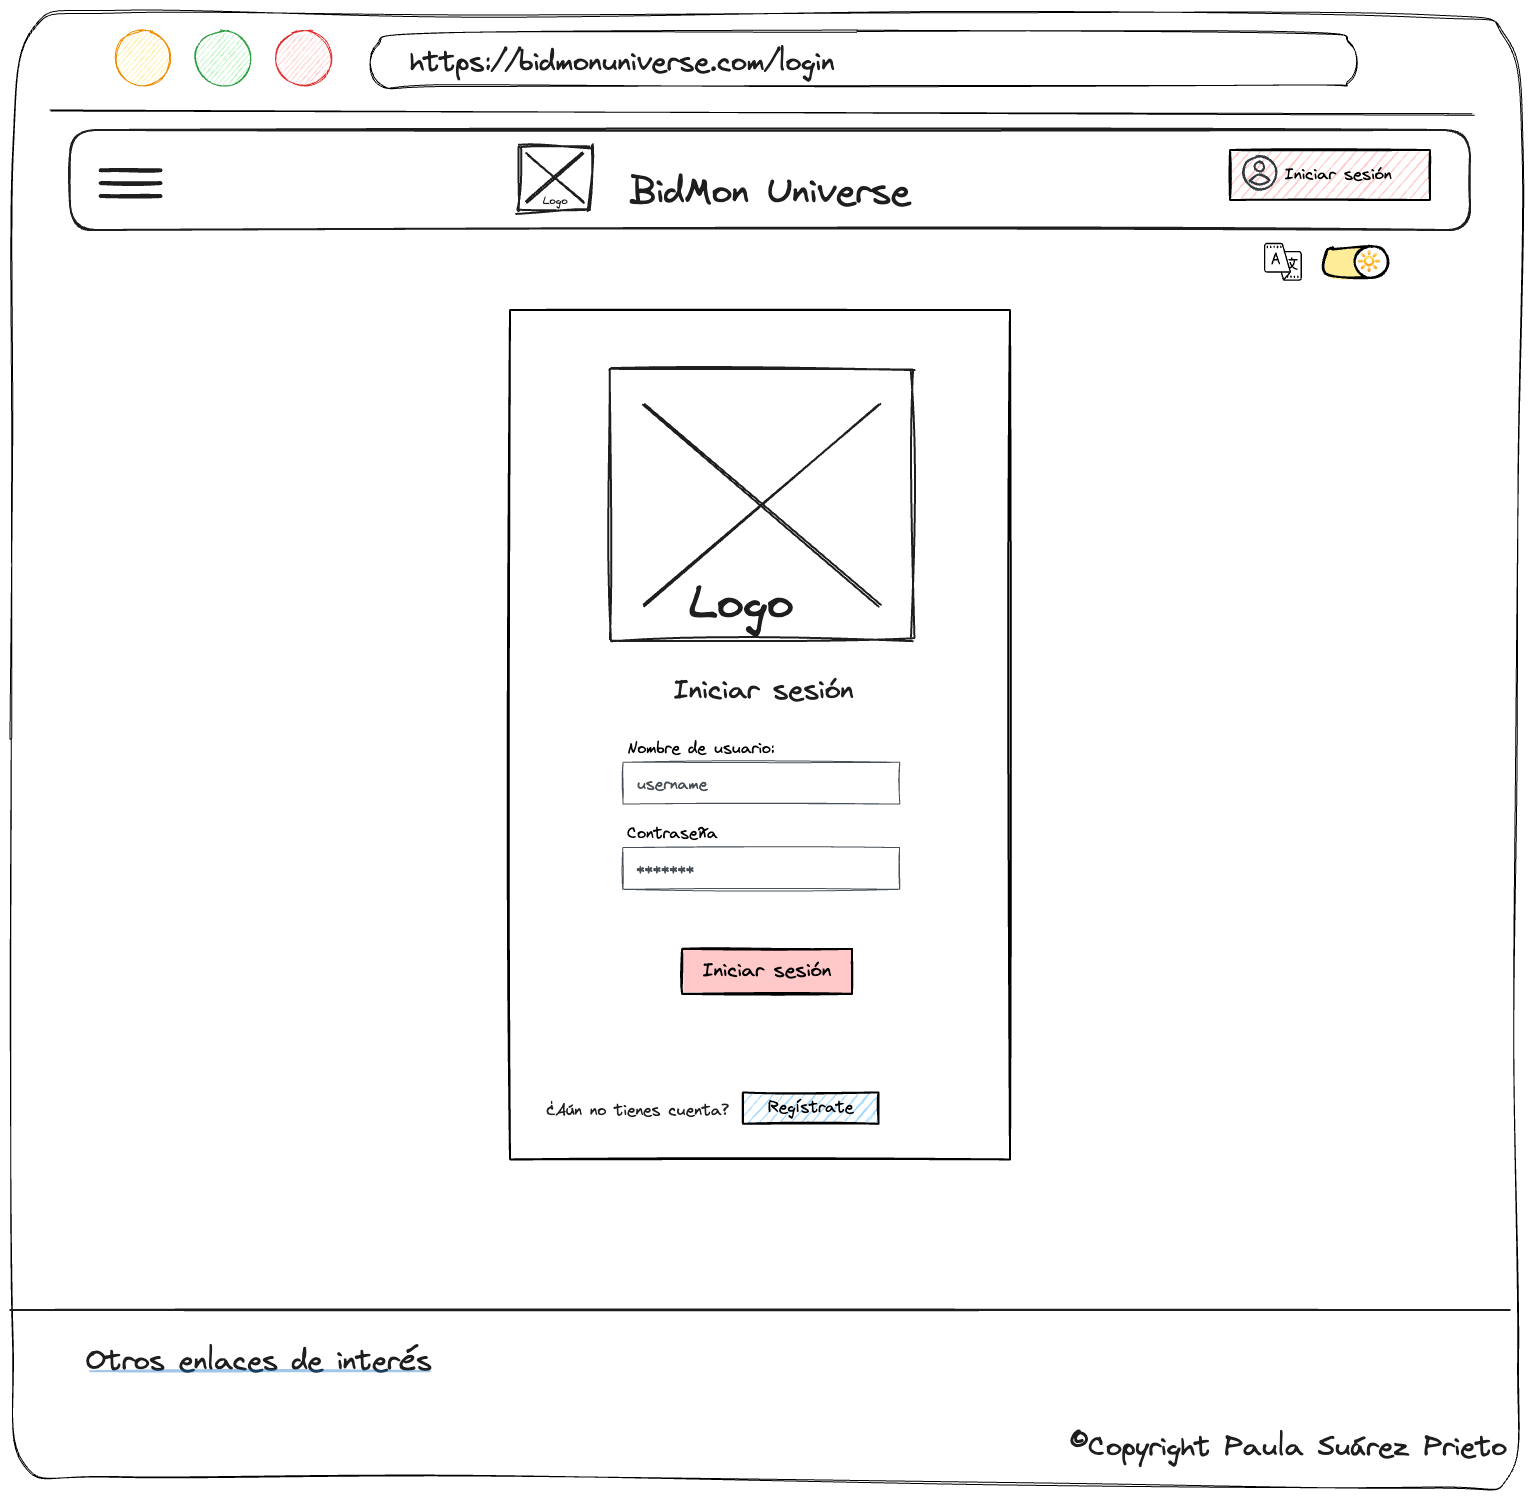
\includegraphics[width=0.8\textwidth]{figures/6-Analisis/6-Interfaz/prototipos/login.png}
    \caption{Boceto de la página de inicio de sesión}
    \label{fig:p_login}
\end{figure}

\subsubsection{Página de Registro}
La página de registro muestra un formulario que permite al usuario crear una cuenta en el sistema o iniciar sesión si ya tiene una cuenta.
En la figura \ref{fig:p_signup} se muestra el boceto de la página de registro.

En caso de que los campos del formulario no cumplan con las restricciones especificadas, se mostrará un mensaje de error y se resaltarán los campos correspondientes.

\begin{figure}[H]
    \centering
    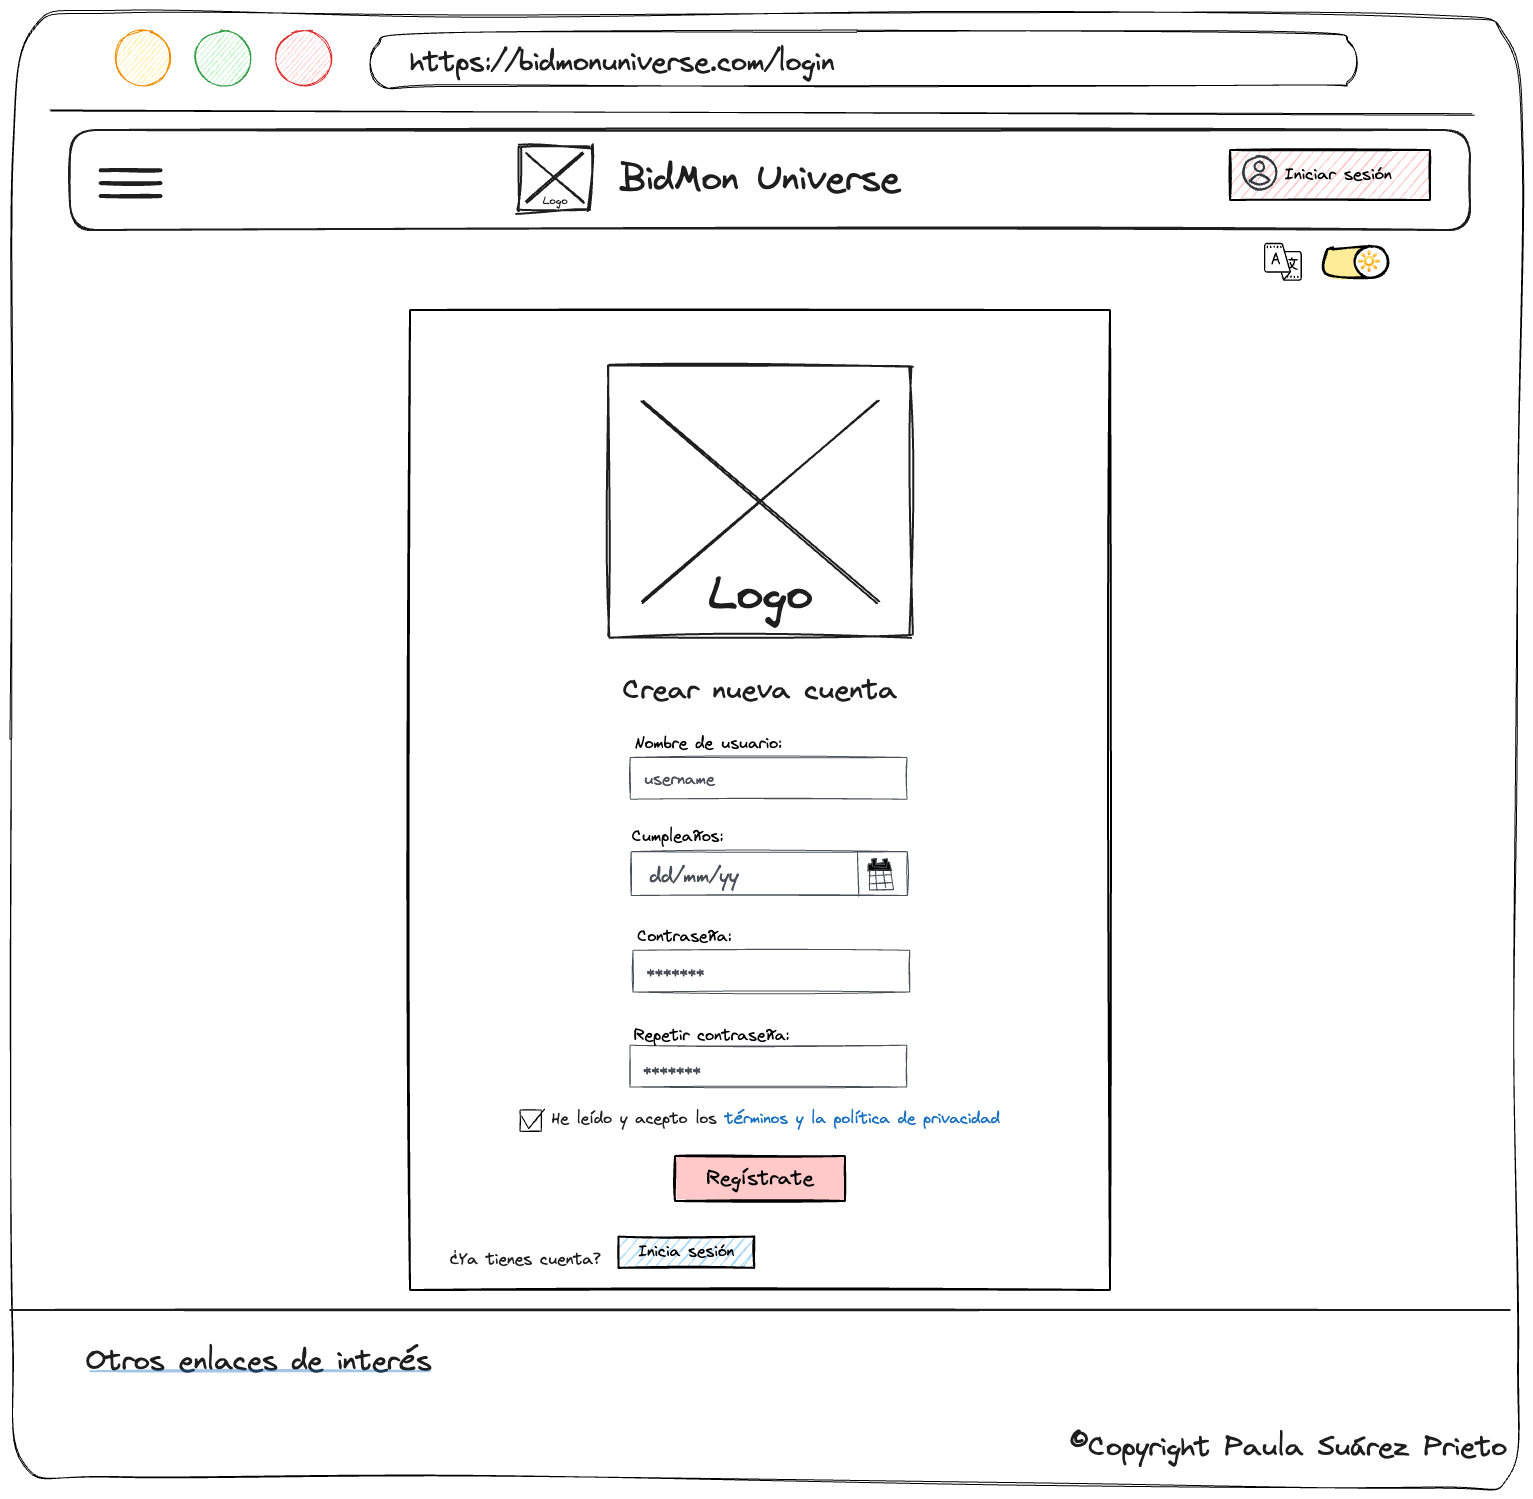
\includegraphics[width=0.8\textwidth]{figures/6-Analisis/6-Interfaz/prototipos/signup.png}
    \caption{Boceto de la página de registro}
    \label{fig:p_signup}
\end{figure}

\subsubsection{Página inicial de usuario}
Una vez que el usuario ha iniciado sesión en la plataforma, se le redirige a la página inicial de usuario.
Las páginas a las que tiene acceso un usuario autenticado muestran siempre como cabecera de la página un menú general de navegación que le permite acceder a las diferentes secciones del sistema,
el saldo de su cuenta y un menú de usuario que le permite acceder a su perfil y cerrar sesión.
La página inicial de usuario muestra un resumen de la información más relevante para el usuario:
\begin{itemize}
    \item Menú de acceso rápido a las secciones principales del sistema.
    \item Muestra las cartas más recientes de su colección con la posibilidad de acceder a la colección completa.
    \item Muestra las subastas activas iniciadas por el usuario más recientes con la posibilidad de acceder a las subastas completas.
    \item Muestra las pujas activas más recientes realizadas por el usuario con la posibilidad de acceder a las pujas completas.
\end{itemize}

En la figura \ref{fig:p_user_home} se muestra el boceto de la página inicial de usuario.

\begin{figure}[H]
    \centering
    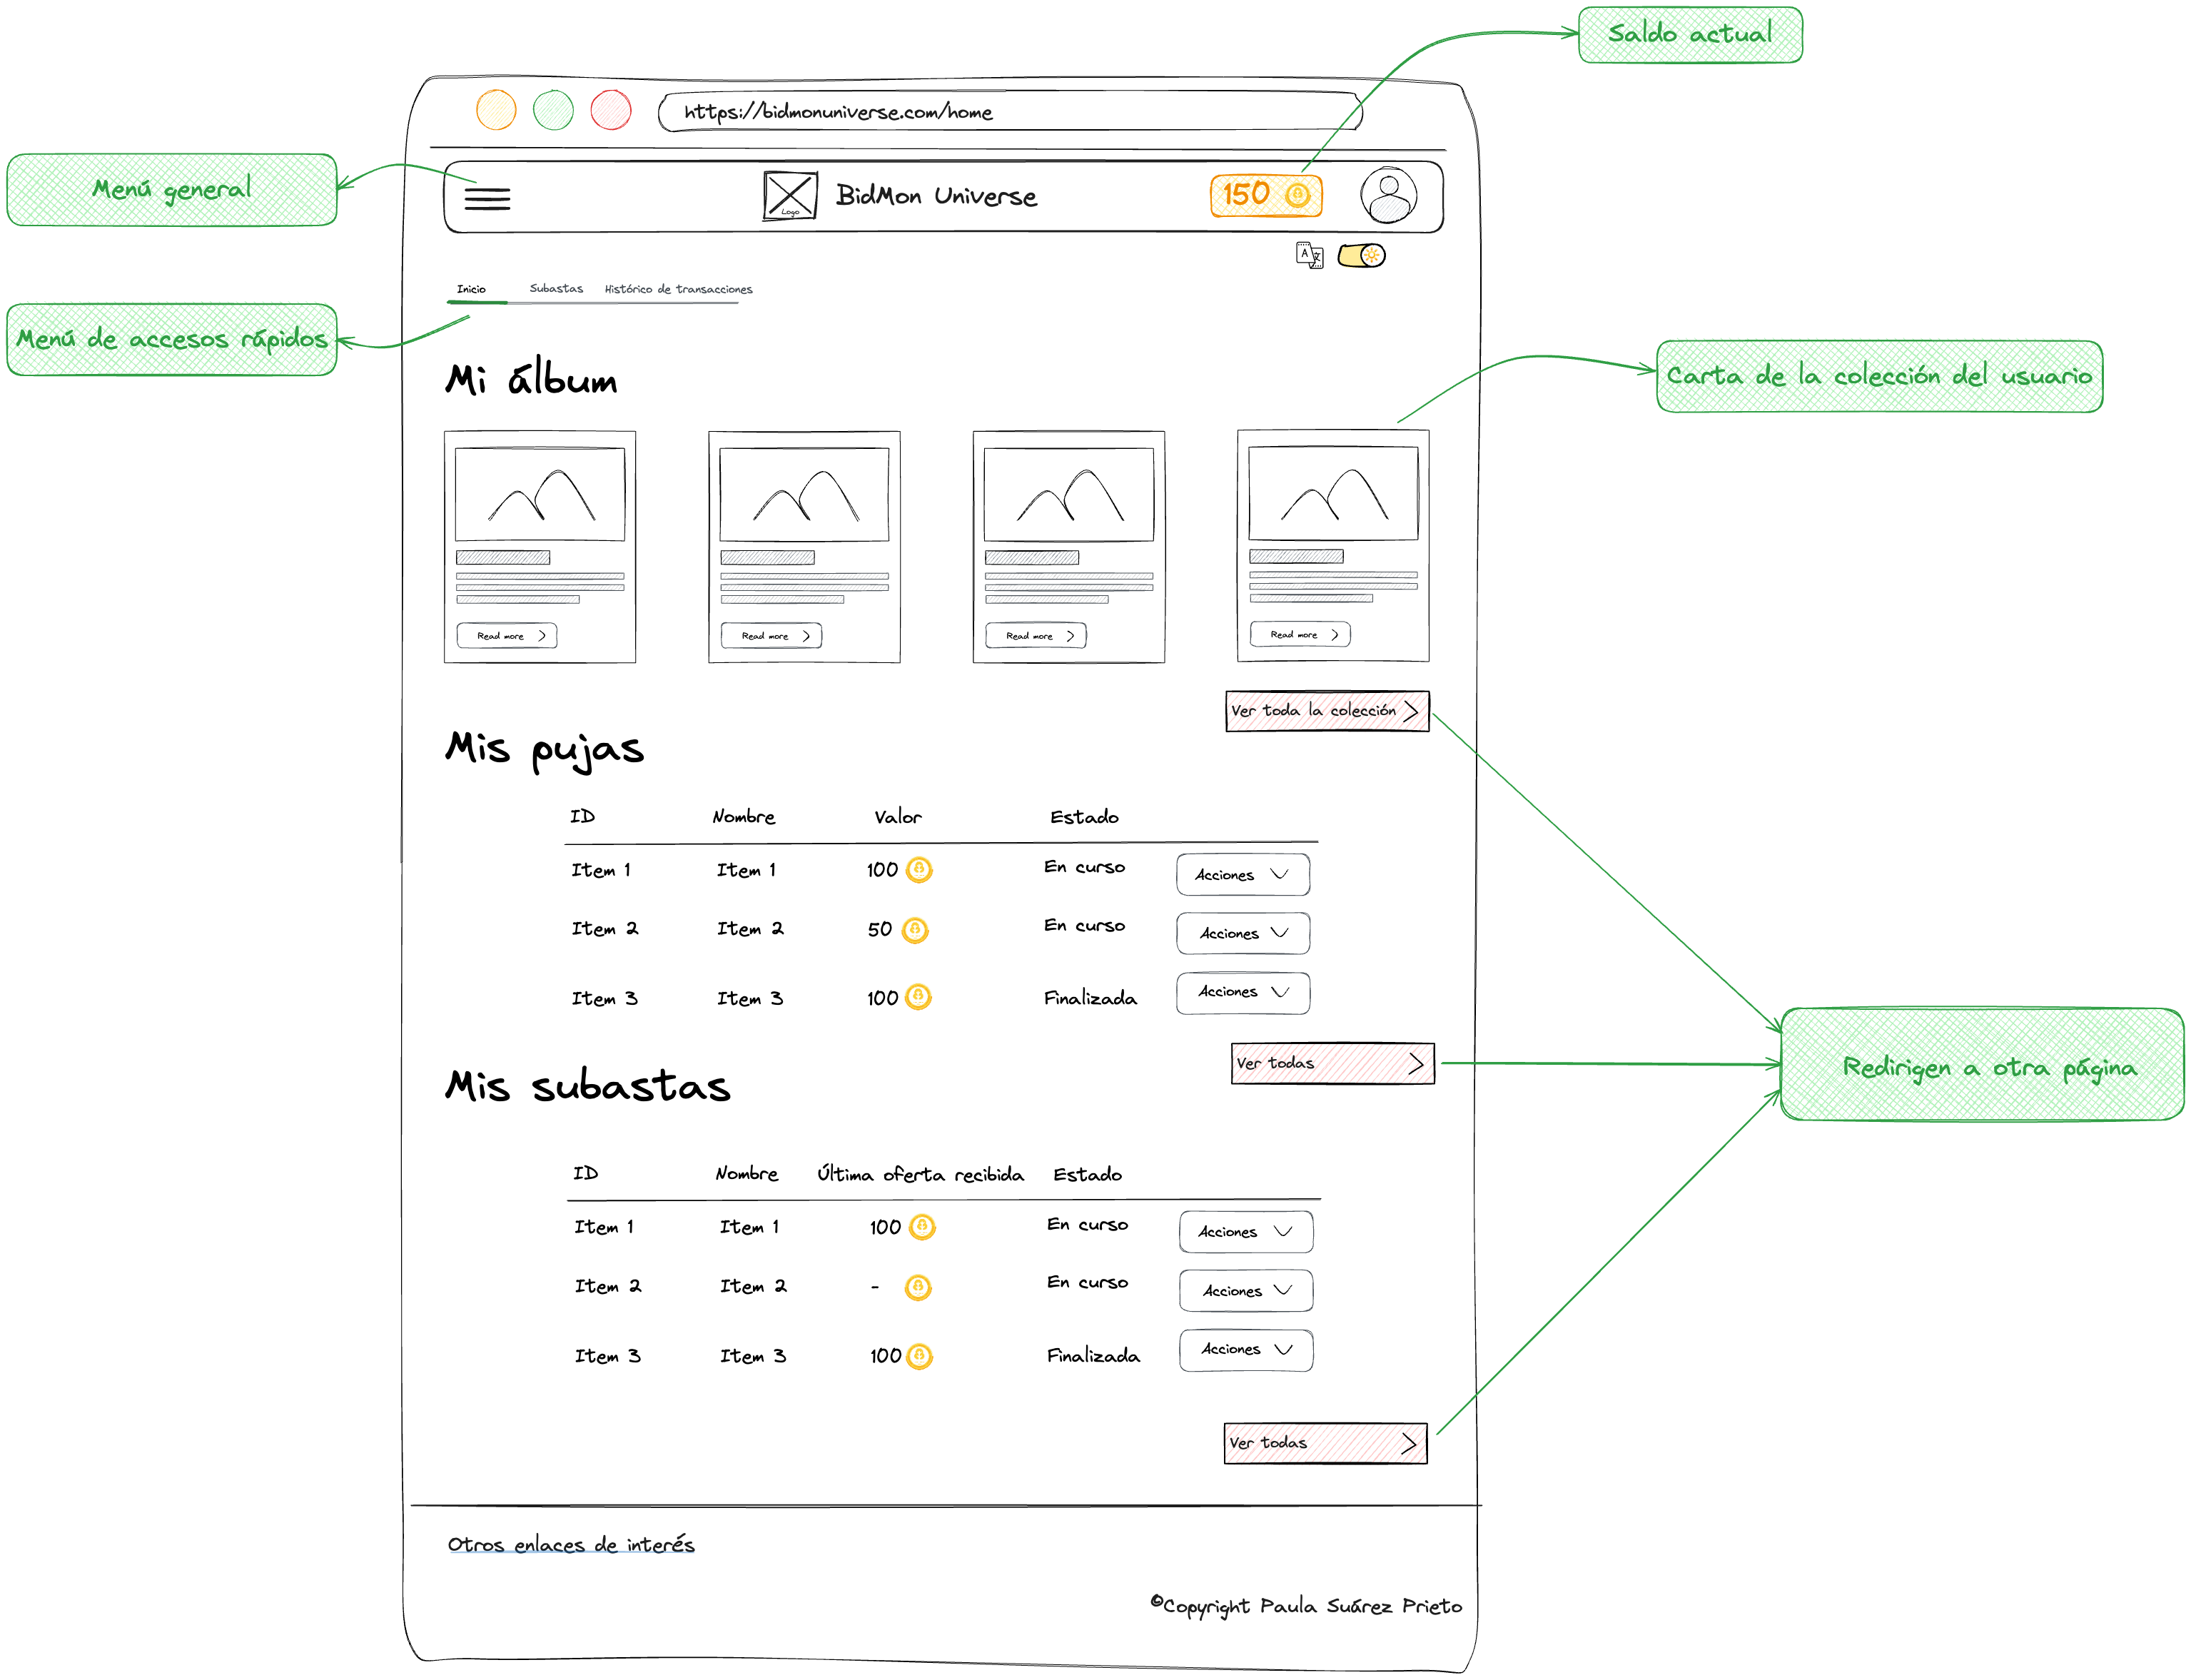
\includegraphics[width=1\textwidth]{figures/6-Analisis/6-Interfaz/prototipos/home-logueada.png}
    \caption{Boceto de la página inicial de usuario}
    \label{fig:p_user_home}
\end{figure}

\subsubsection{Página de Colección}
La página de colección muestra una lista de las cartas que el usuario ha añadido a su colección.
El usuario puede hacer clic en una carta para ver más detalles sobre ella.
En la figura \ref{fig:p_collection} se muestra el boceto de la página de colección.
\begin{figure}[H]
    \centering
    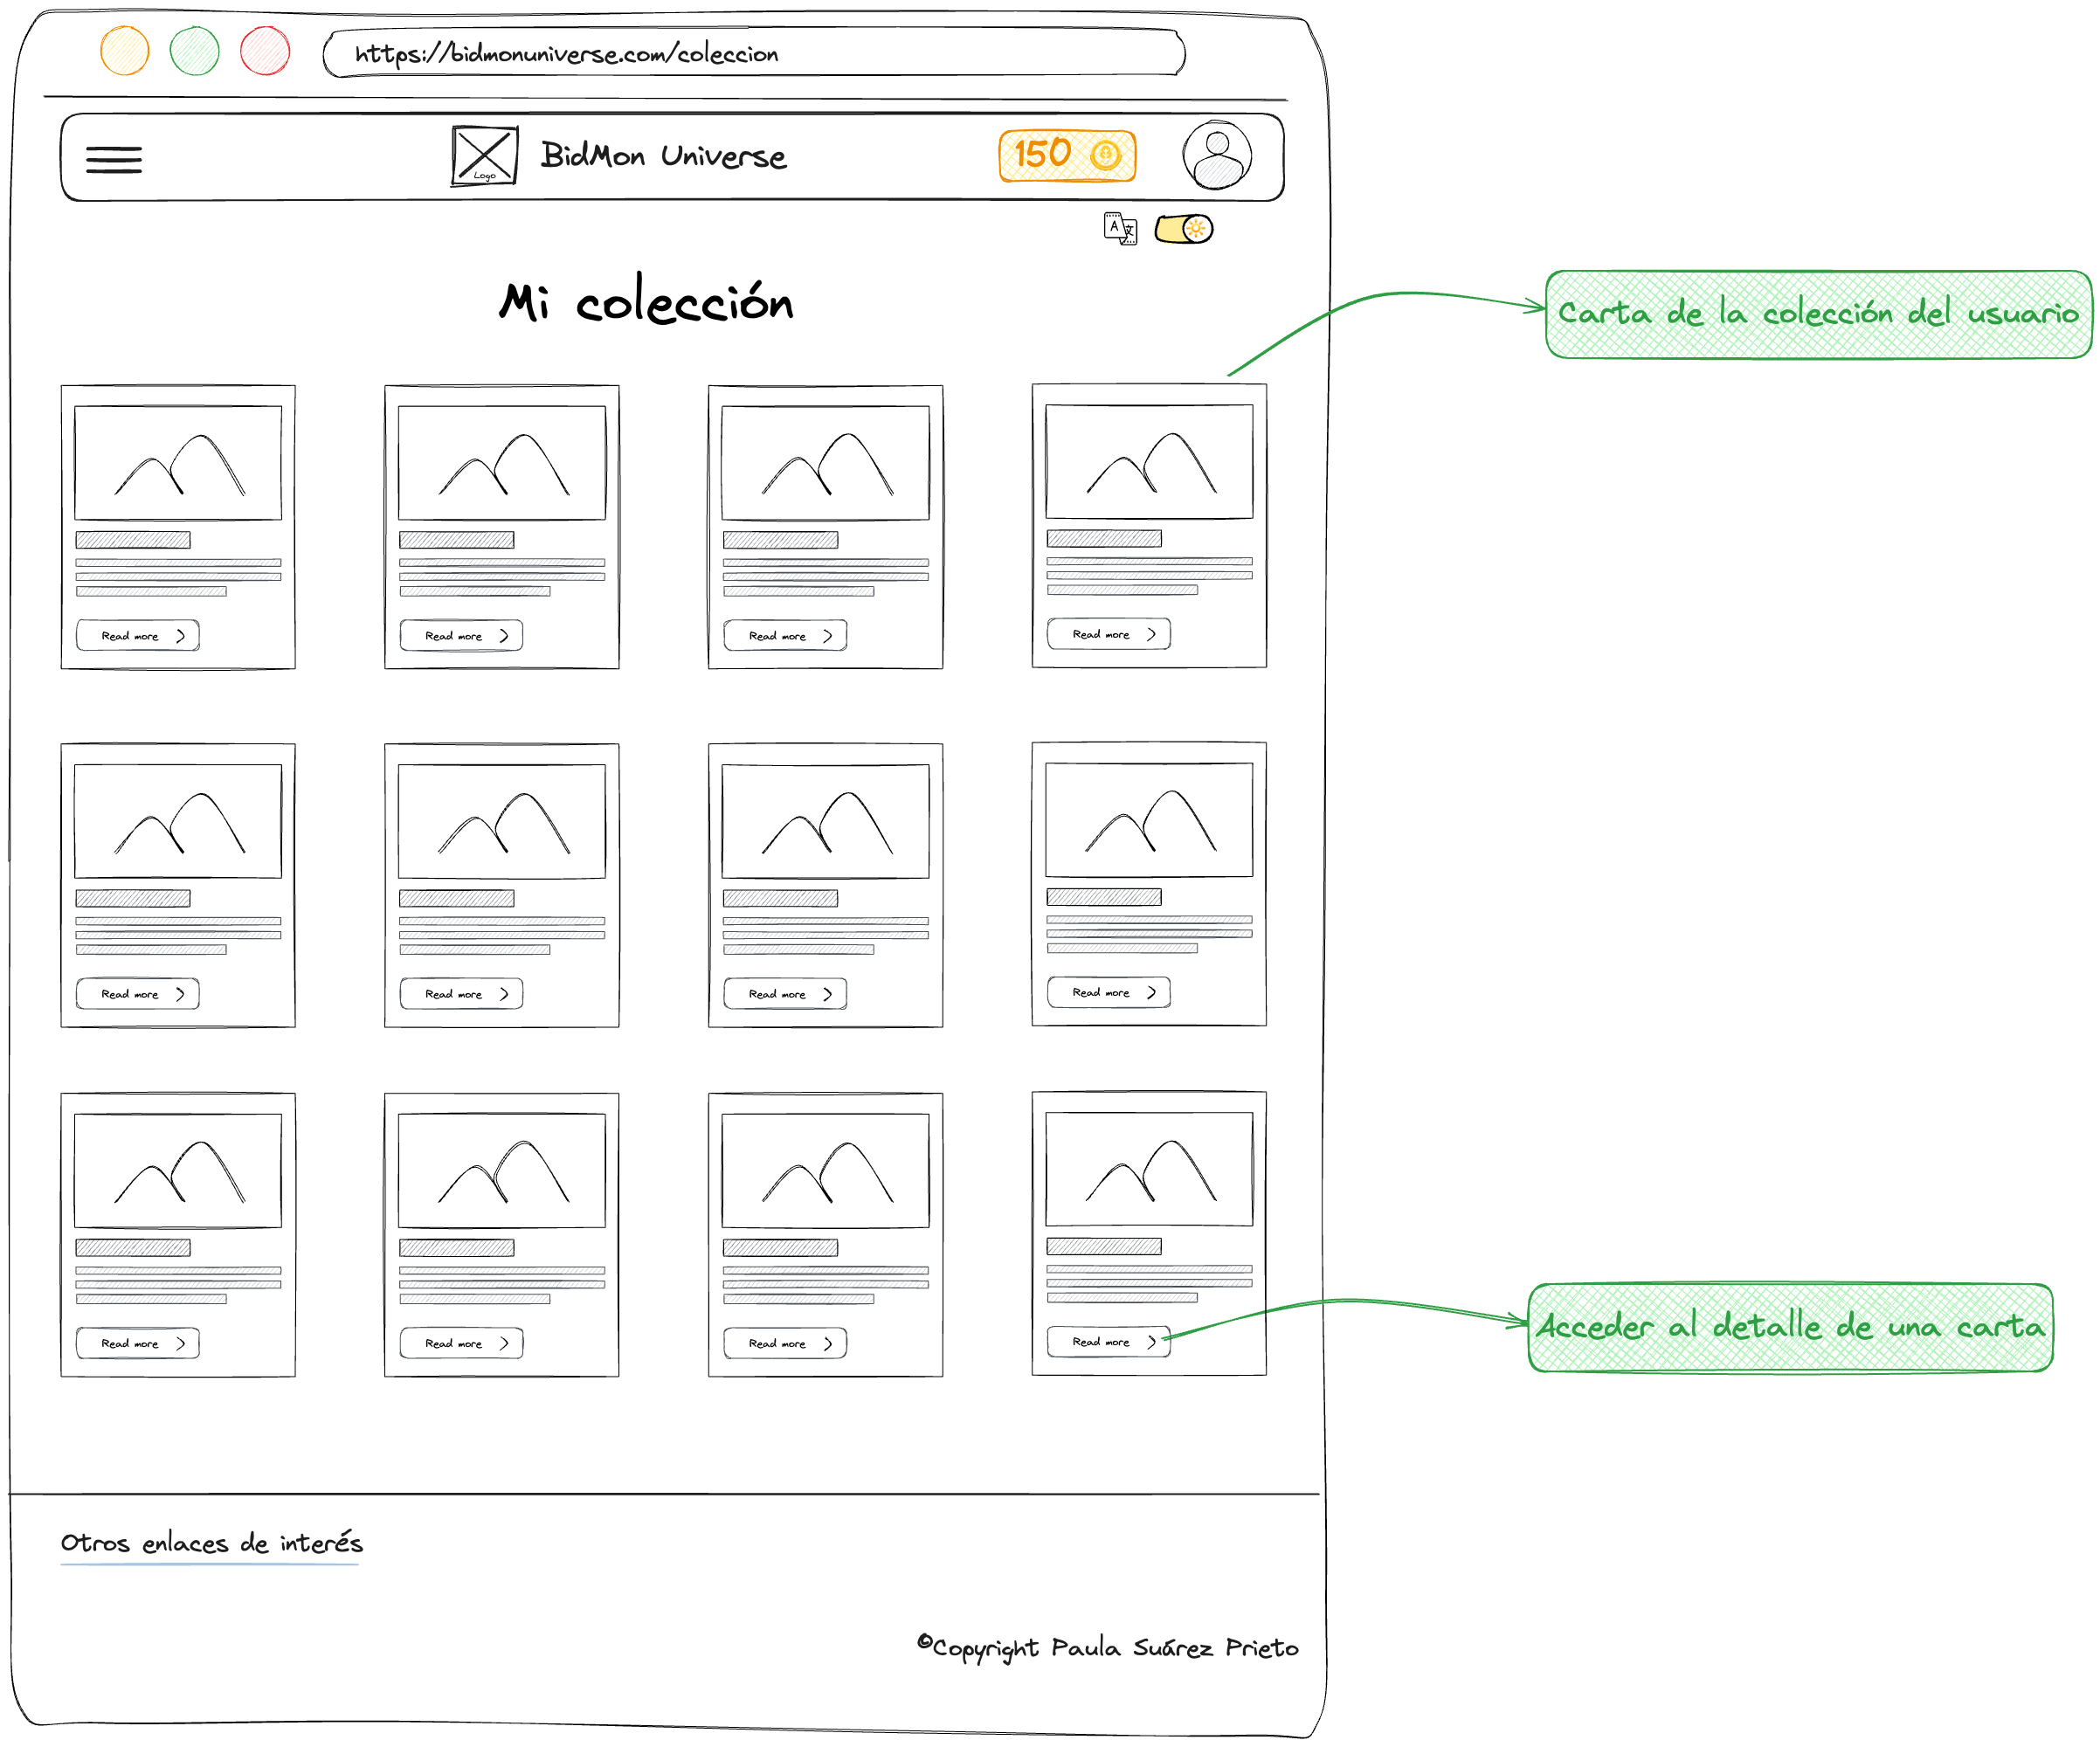
\includegraphics[width=0.9\textwidth]{figures/6-Analisis/6-Interfaz/prototipos/coleccion.png}
    \caption{Boceto de la página de colección}
    \label{fig:p_collection}
\end{figure}

\subsubsection{Página de Detalles de Carta}
La página de detalles de carta muestra información detallada sobre una carta específica. Permite al usuario ver la imagen de la carta, los datos de la carta, 
las transacciones de esta y la posibilidad de marcar la carta como destacada o subastarla.
En la figura \ref{fig:p_card_details} se muestra el boceto de la página de detalles de carta.
\begin{figure}[H]
    \centering
    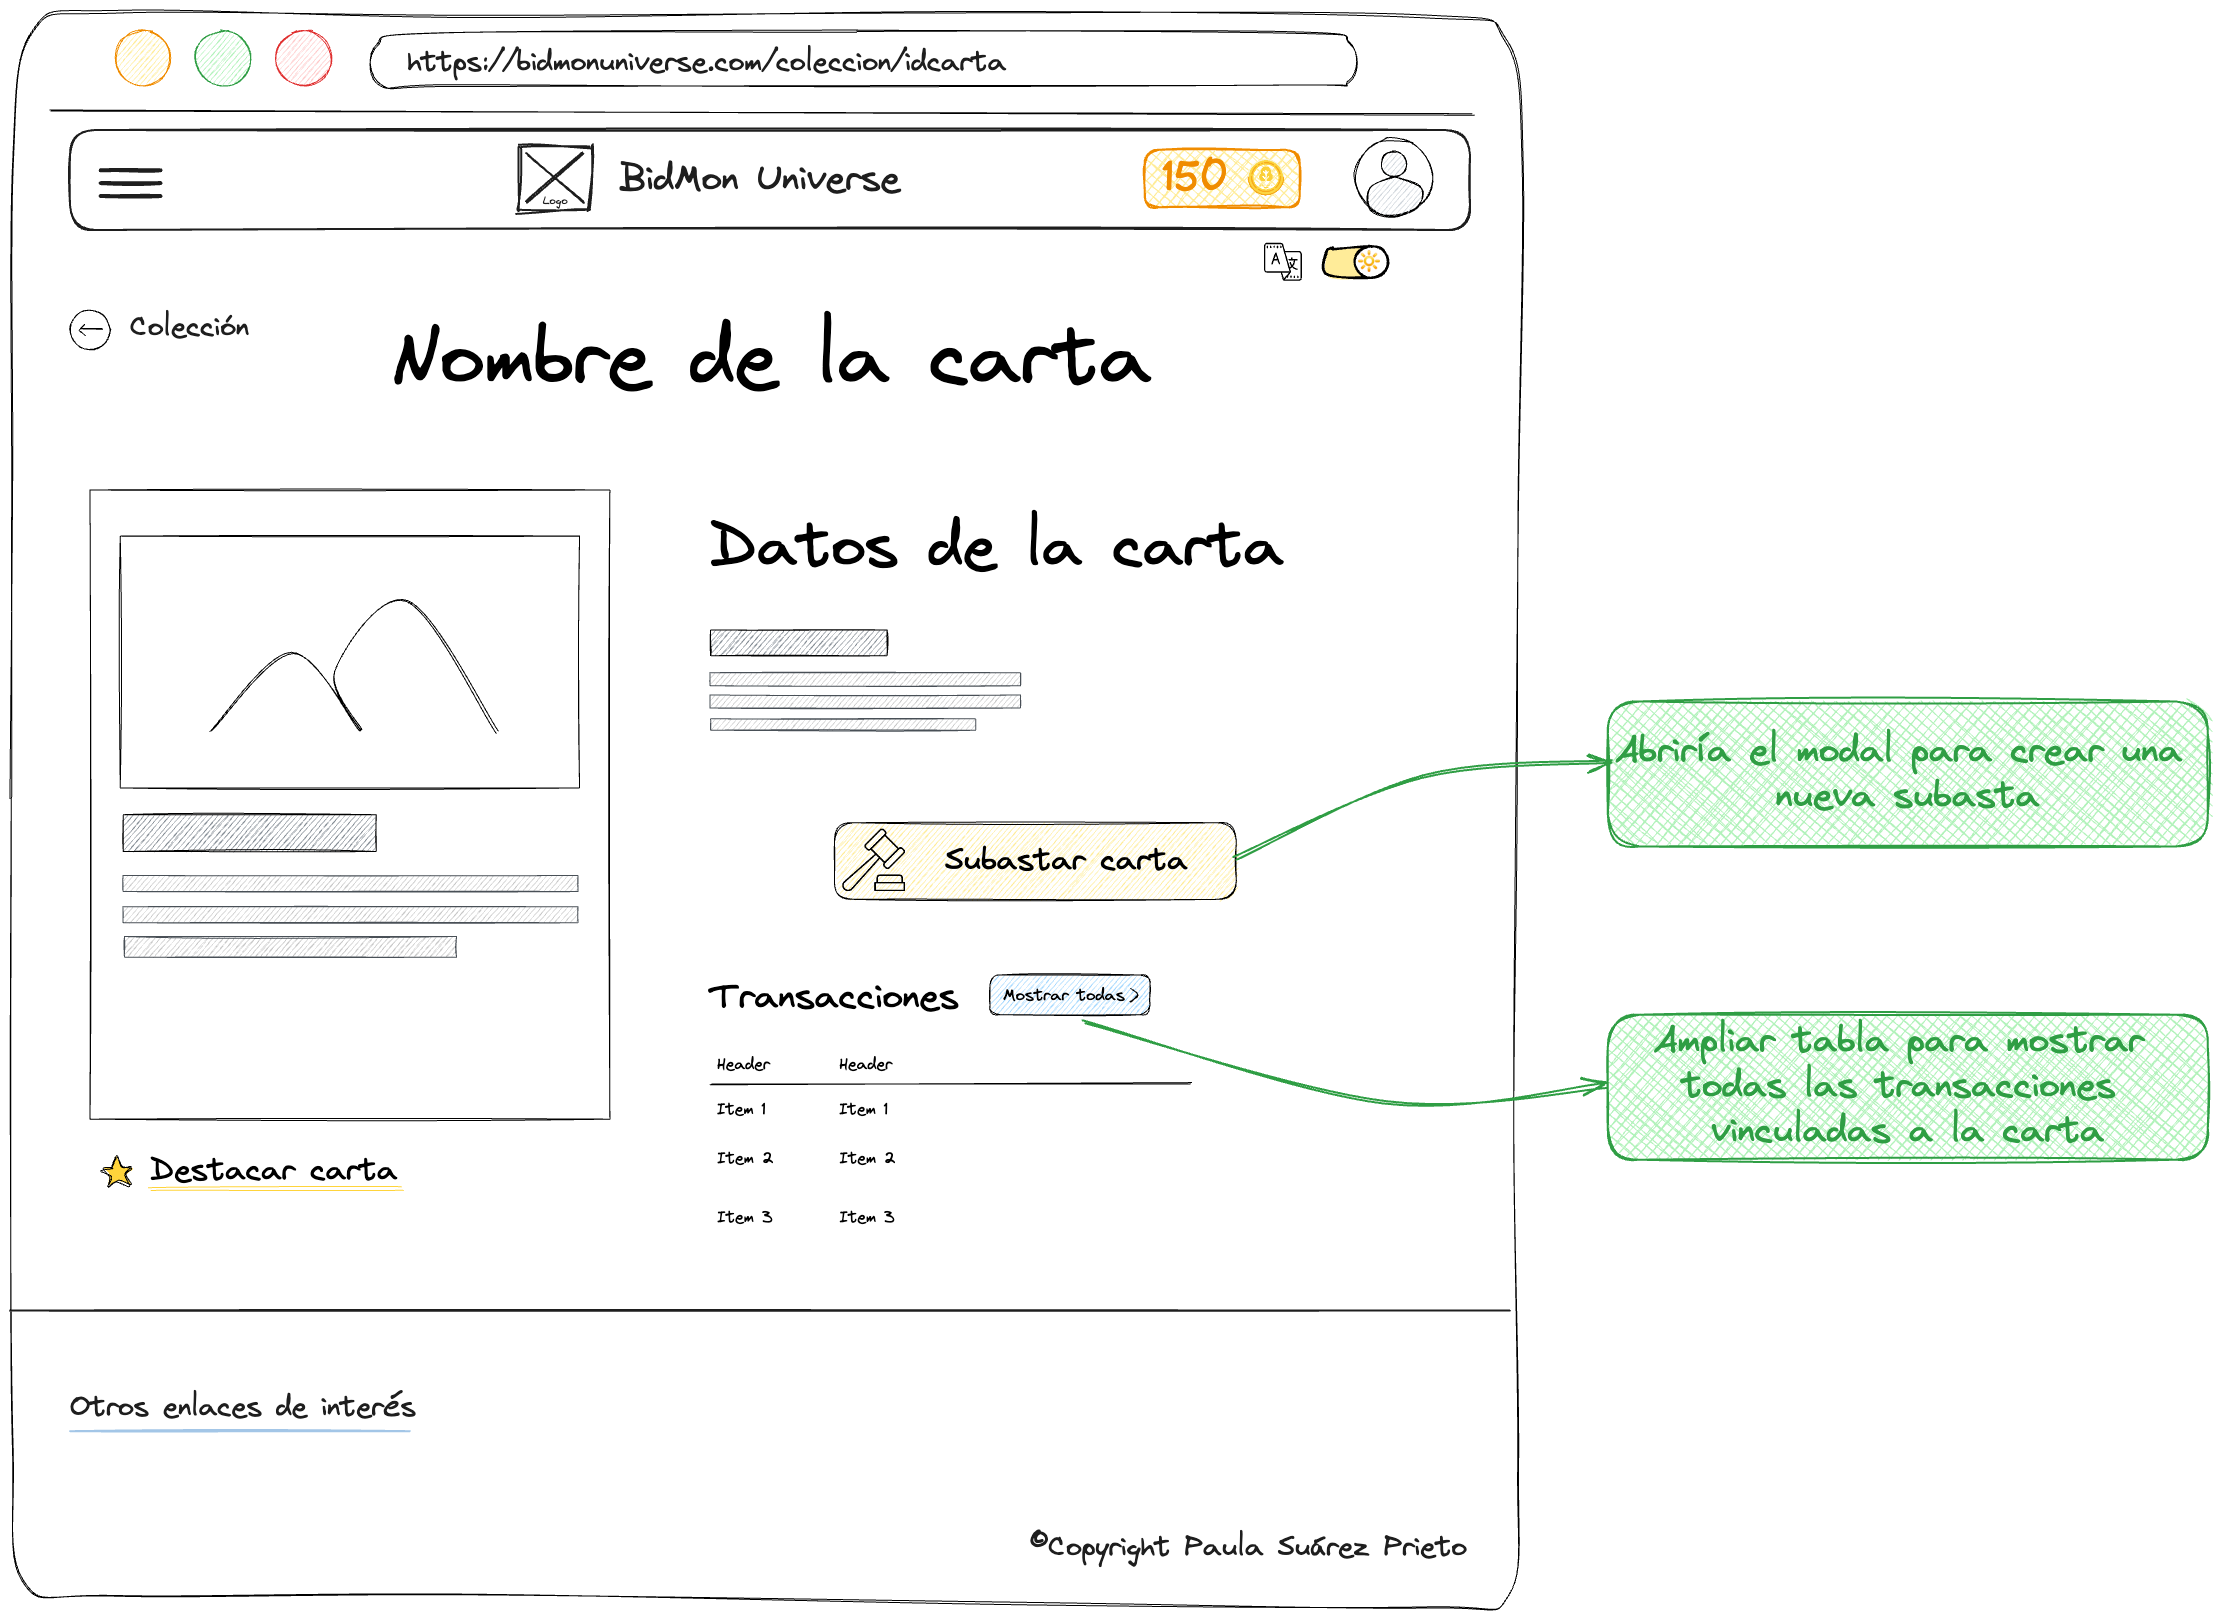
\includegraphics[width=0.9\textwidth]{figures/6-Analisis/6-Interfaz/prototipos/detalle-carta.png}
    \caption{Boceto de la página de detalles de carta}
    \label{fig:p_card_details}
\end{figure}

\subsubsection{Página de Subastas}
La página de subastas muestra una lista de las subastas activas en las que el usuario puede participar.
En esta página hay un menú de navegación que permite al usuario filtrar las subastas por diferentes criterios:
\begin{itemize}
    \item Todas: Todas las subastas activas.
    \item Mis Subastas: Subastas en las que el usuario ha creado.
    \item Pujas: Subastas en las que el usuario ha pujado.
\end{itemize}
La página de subastas muestra las cartas subastadas, al hacer clic en una carta se muestra la información detallada de la subasta.
En la figura \ref{fig:p_auctions} se muestra el boceto de la página de subastas.
\begin{figure}[H]
    \centering
    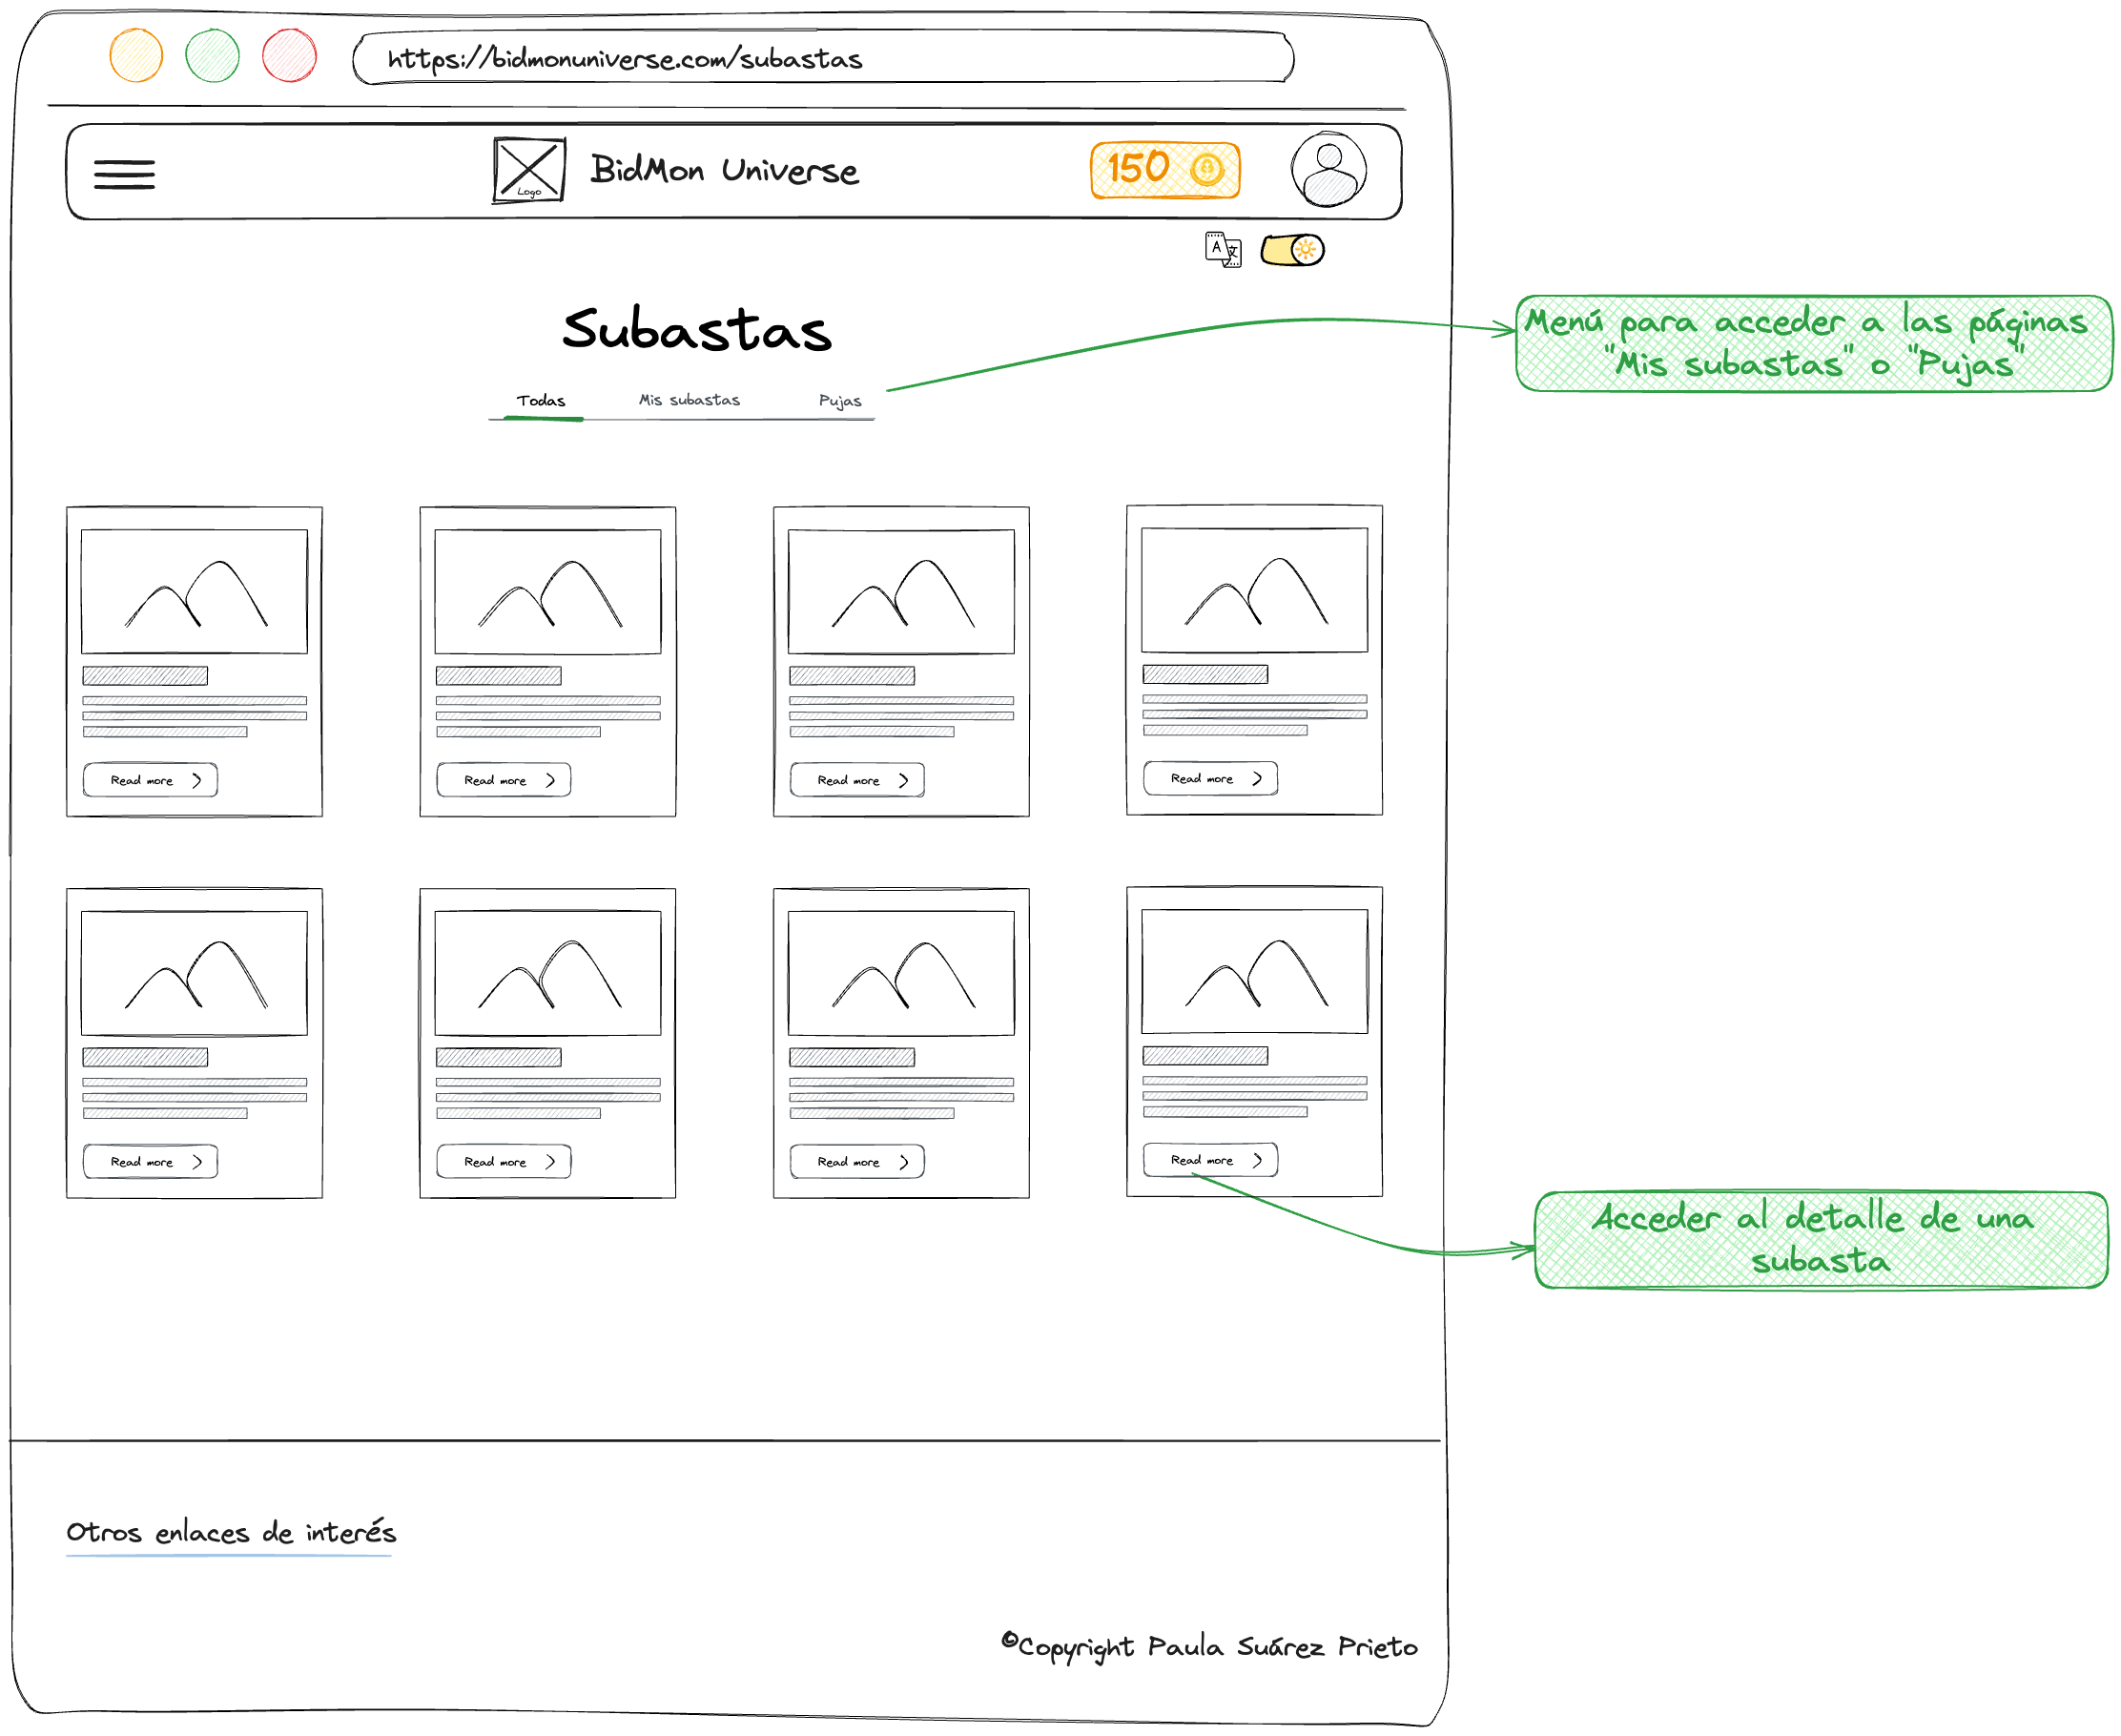
\includegraphics[width=0.9\textwidth]{figures/6-Analisis/6-Interfaz/prototipos/subastas.png}
    \caption{Boceto de la página de subastas}
    \label{fig:p_auctions}
\end{figure}

\subsubsection{Página de Detalles de Subasta}
La página de detalles de subasta muestra información detallada sobre una subasta específica.
Dependiendo de si la subasta es propia o no, el usuario puede realizar diferentes acciones.
En la figura \ref{fig:p_auction_details} se muestra el boceto de la página de detalles de una subasta activa creada por otro usuario.
\begin{figure}[H]
    \centering
    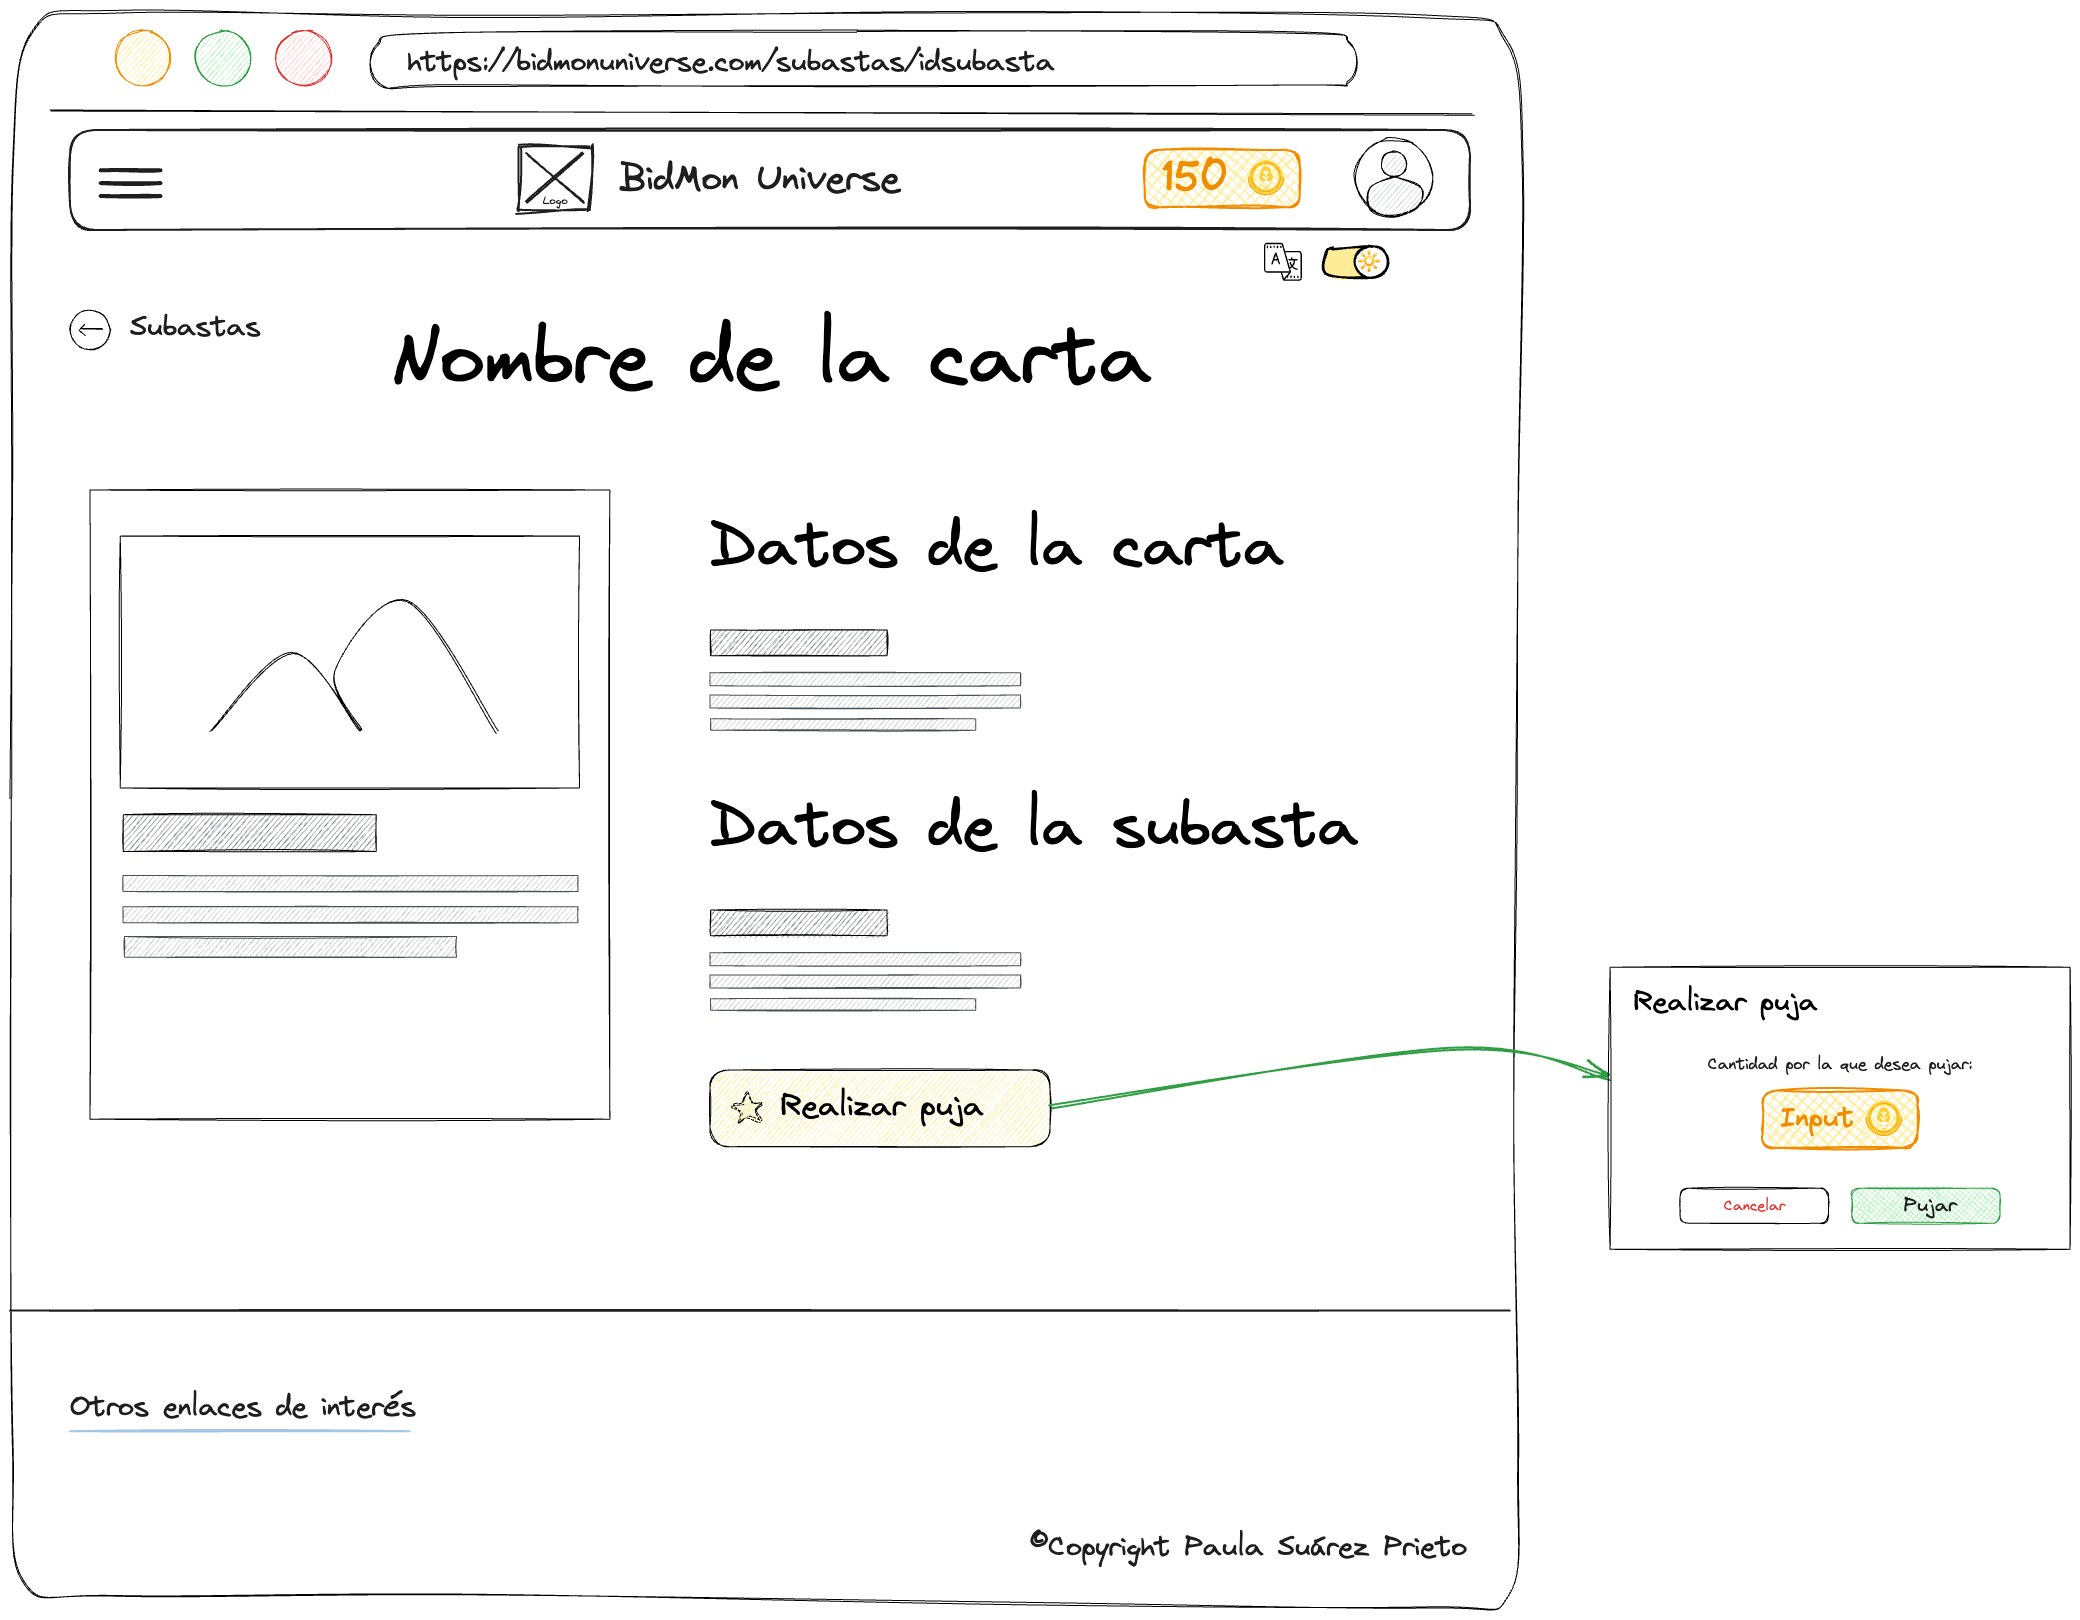
\includegraphics[width=0.9\textwidth]{figures/6-Analisis/6-Interfaz/prototipos/detalle-subasta.png}
    \caption{Boceto de la página de detalles de subasta}
    \label{fig:p_auction_details}
\end{figure}

En el caso de que la subasta sea propia, el usuario puede cancelar la subasta como se muestra en la figura \ref{fig:p_auction_details_own}.
\begin{figure}[H]
    \centering
    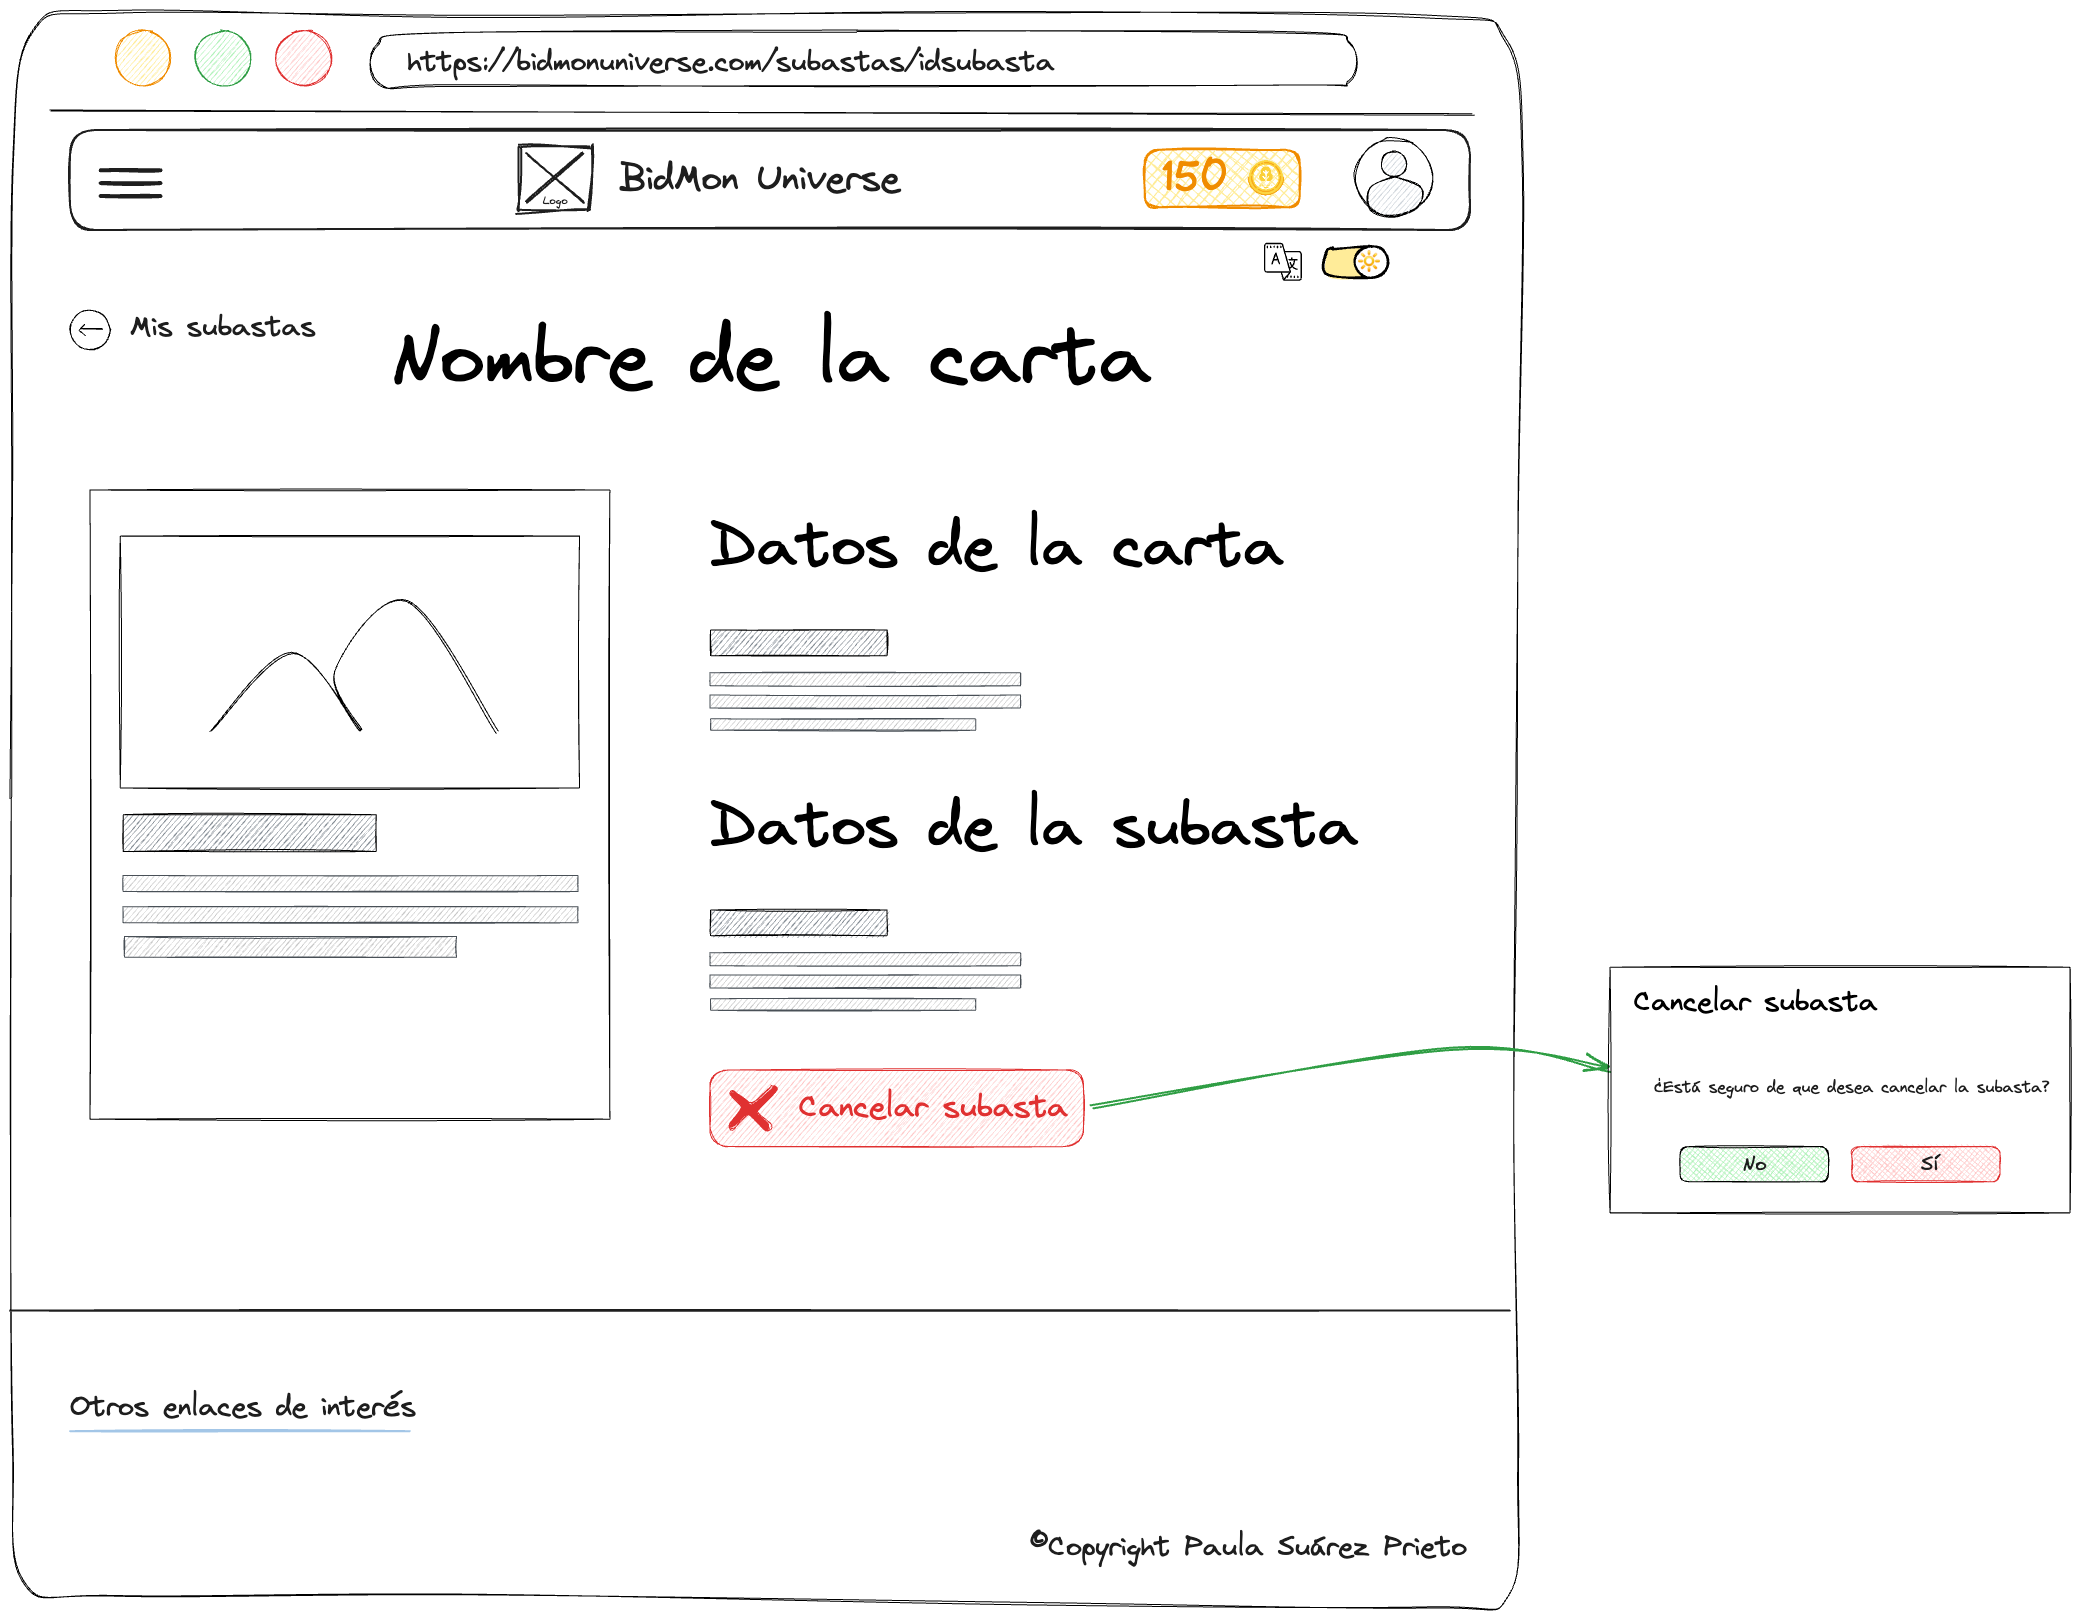
\includegraphics[width=0.9\textwidth]{figures/6-Analisis/6-Interfaz/prototipos/detalle-subasta-propia.png}
    \caption{Boceto de la página de detalles de subasta propia}
    \label{fig:p_auction_details_own}
\end{figure}

En el caso de que sea una subasta en la que el usuario ha pujado, el usuario puede retirar la puja como se muestra en la figura \ref{fig:p_auction_details_bid}.
\begin{figure}[H]
    \centering
    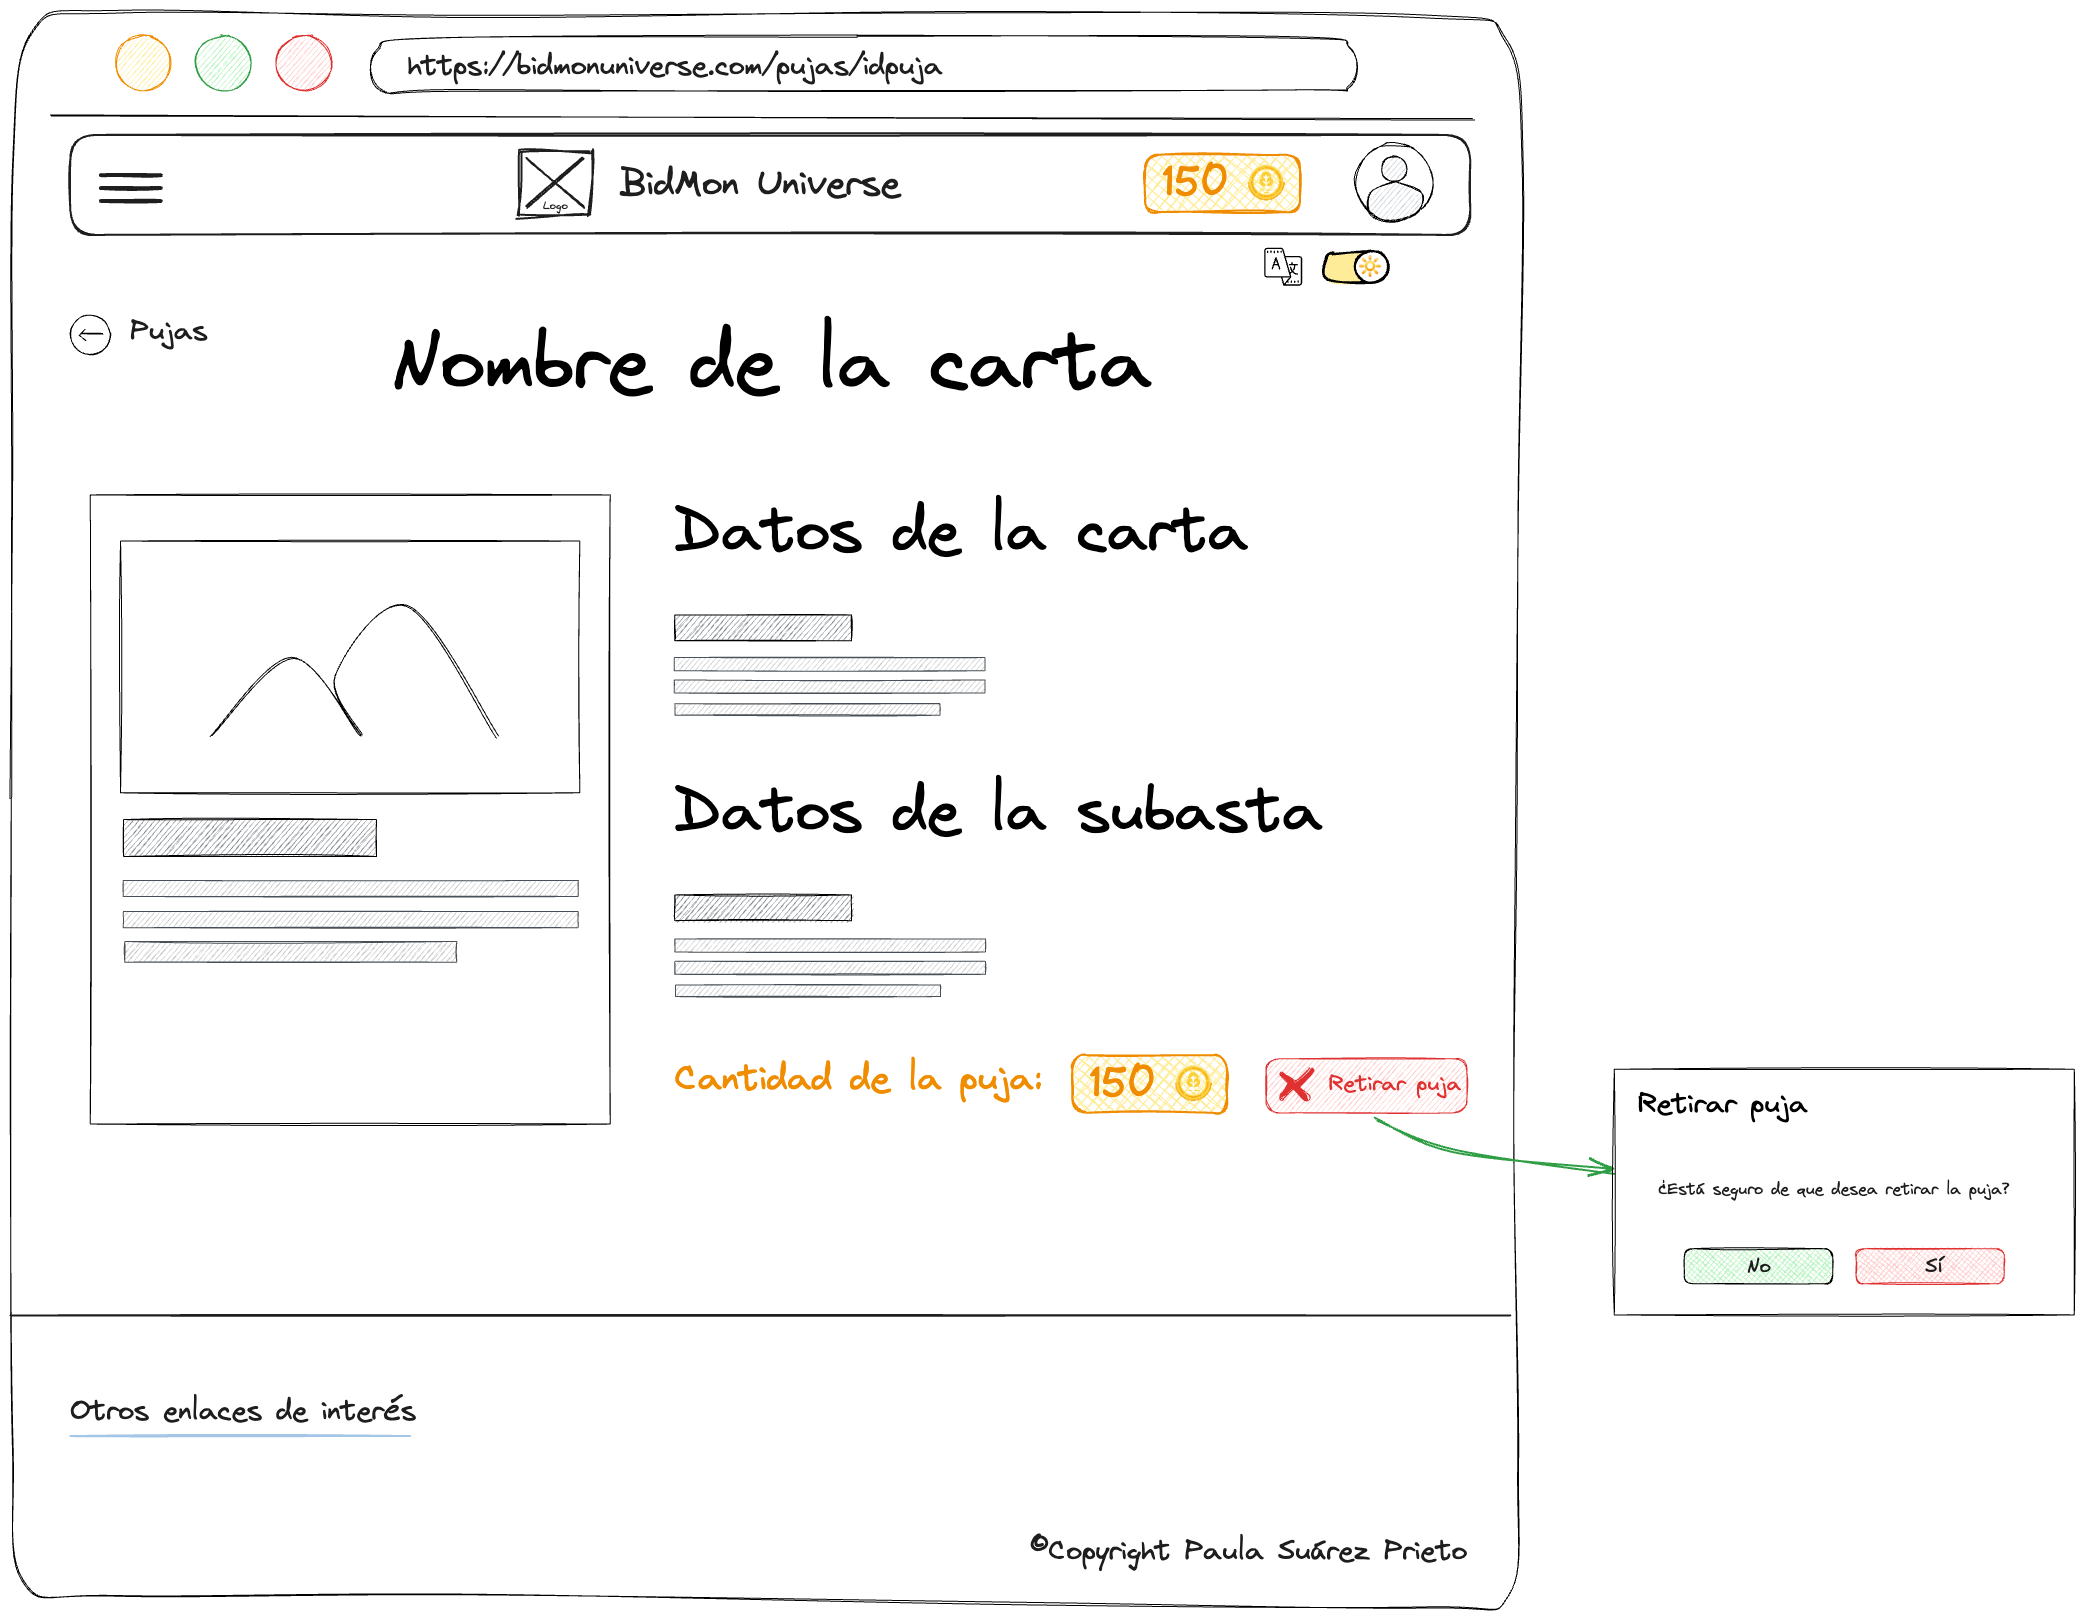
\includegraphics[width=0.9\textwidth]{figures/6-Analisis/6-Interfaz/prototipos/detalle-puja.png}
    \caption{Boceto de la página de detalles de subasta en la que el usuario ha pujado}
    \label{fig:p_auction_details_bid}
\end{figure}

\subsubsection{Página de Histórico de Transacciones}
La página de histórico de transacciones muestra una lista de las transacciones realizadas.
Si el usuario que ha iniciado sesión es un administrador, se mostrarán todas las transacciones realizadas en el sistema.
Si el usuario que ha iniciado sesión es un usuario normal, se mostrarán solo las transacciones realizadas por él.
En la figura \ref{fig:p_transactions} se muestra el boceto de la página de histórico de transacciones.
\begin{figure}[H]
    \centering
    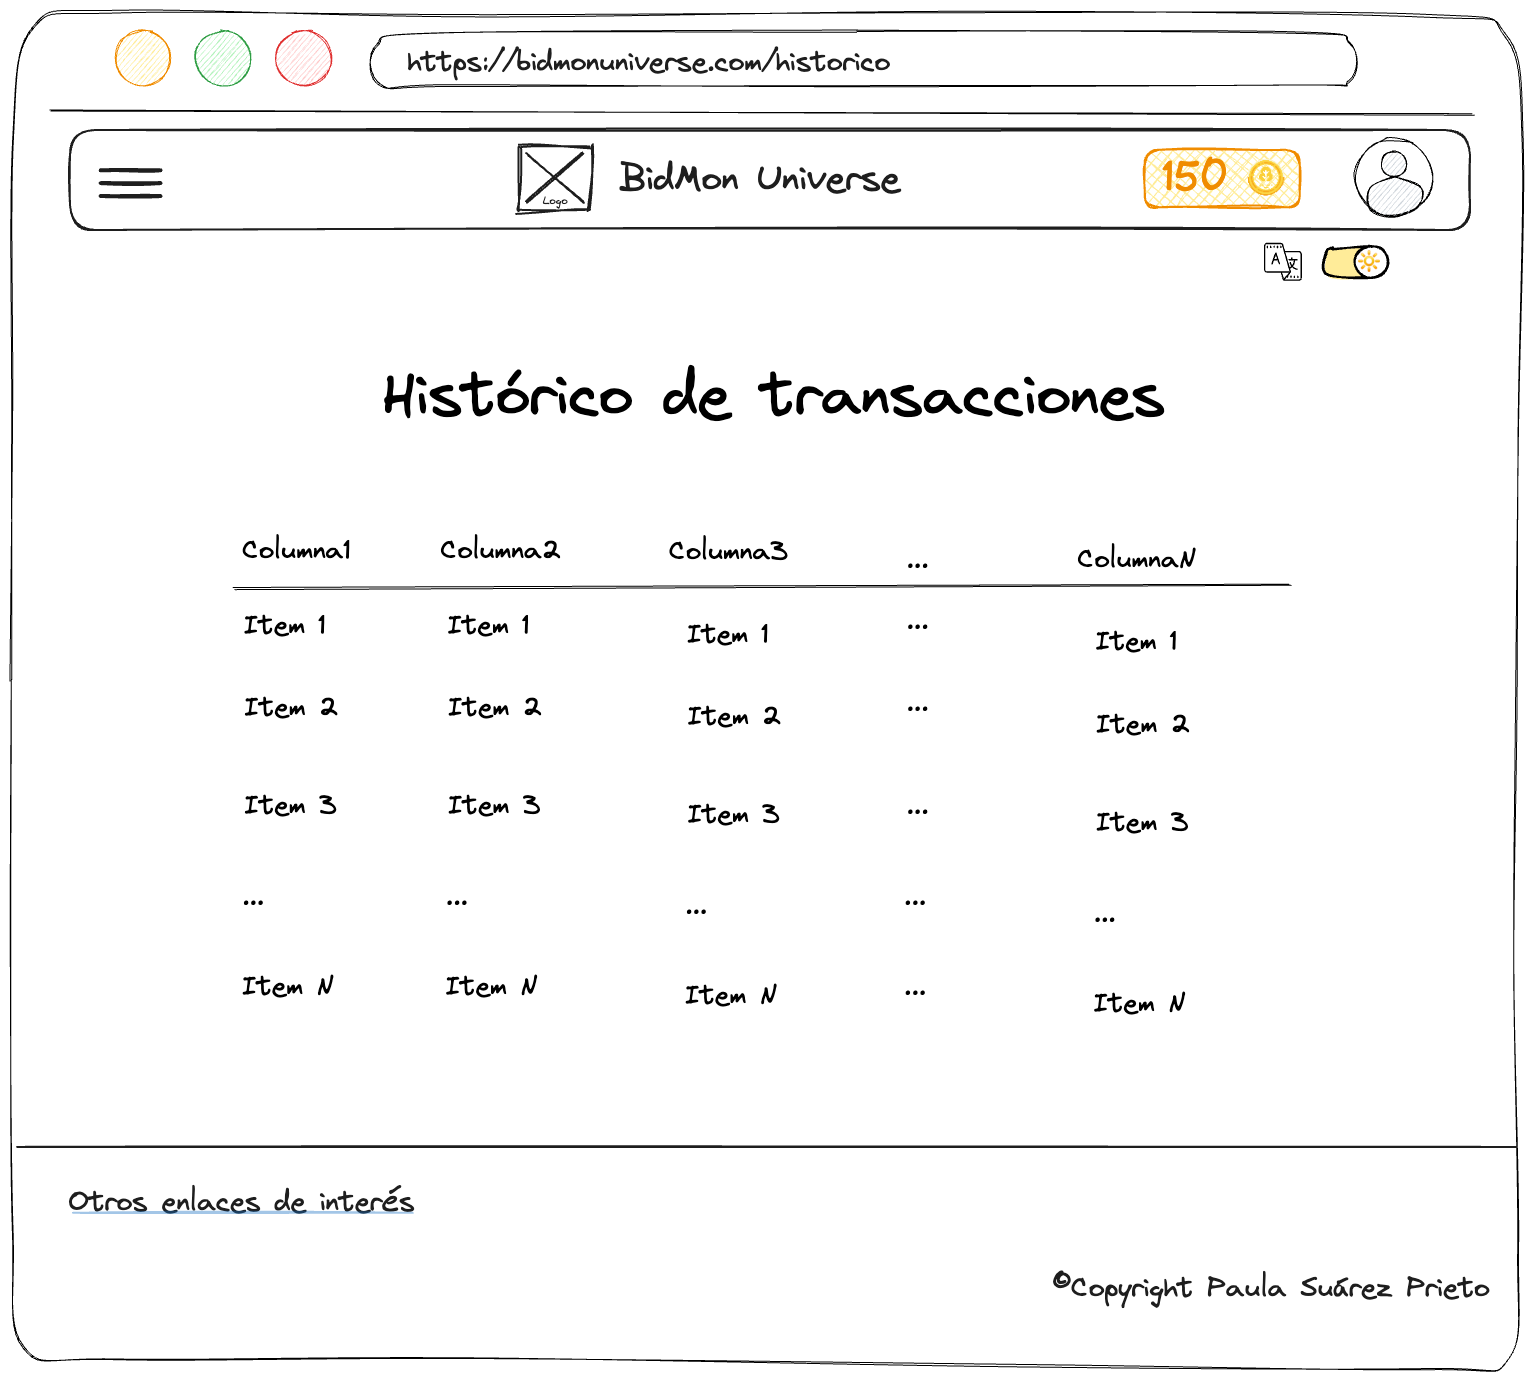
\includegraphics[width=0.9\textwidth]{figures/6-Analisis/6-Interfaz/prototipos/historico-transacciones.png}
    \caption{Boceto de la página de histórico de transacciones}
    \label{fig:p_transactions}
\end{figure}

\subsection{Definición del aspecto de la interfaz}
Se ha creado la interfaz en base a los bocetos de la sección anterior.
La interfaz se ha desarrollado en React.

\subsubsection{Descripción de los recursos empleados en la interfaz}
La primera tarea que se ha realizado ha sido la de definir los colores y tipografías que se van a utilizar en la interfaz.
Se ha elegido la tipografía \textit{Pokemon Hollow} para el título de la aplicación y para la bienvenida al usuario.

El logo de la aplicación se ha generado mediante inteligencia artificial, utilizando la herramienta \coloredUnderline{\href{https://openai.com/chatgpt/}{ChatGPT}}.
, al igual que el \textit{favicon} de la aplicación.

Los avatares que se pueden seleccionar como imagen de perfil se han obtenido de la página web \coloredUnderline{\href{https://www.behance.net/gallery/10774061/Pokmon-Avatars}{Behance, Pokémon Avatars de Mikeel Araña}}.

Las imágenes de las medallas de los gimnasios se han obtenido de la página web \coloredUnderline{\href{https://www.wikidex.net/wiki/Líder_de_gimnasio}{Wikidex}}.

Los iconos de los tipos de Pokémon se han obtenido del repositorio \coloredUnderline{\href{https://github.com/duiker101/pokemon-type-svg-icons}{pokemon-type-svg-icons, de duiker101}}.

Las imágenes de los Pokémon se han obtenido de la página web \coloredUnderline{\href{https://pokeapi.co/}{PokéAPI}}.

Para implementar la interfaz se ha utilizado principalmente la biblioteca \coloredUnderline{\href{https://material-ui.com/}{Material-UI}}. 


\subsubsection{Interfaz de la aplicación}
A continuación se muestran las pantallas de las páginas principales de la aplicación.
Pueden diferir ligeramente de los bocetos iniciales, ya que se han realizado ajustes para mejorar la usabilidad y la estética de la aplicación.

\begin{figure}[H]
    \centering
    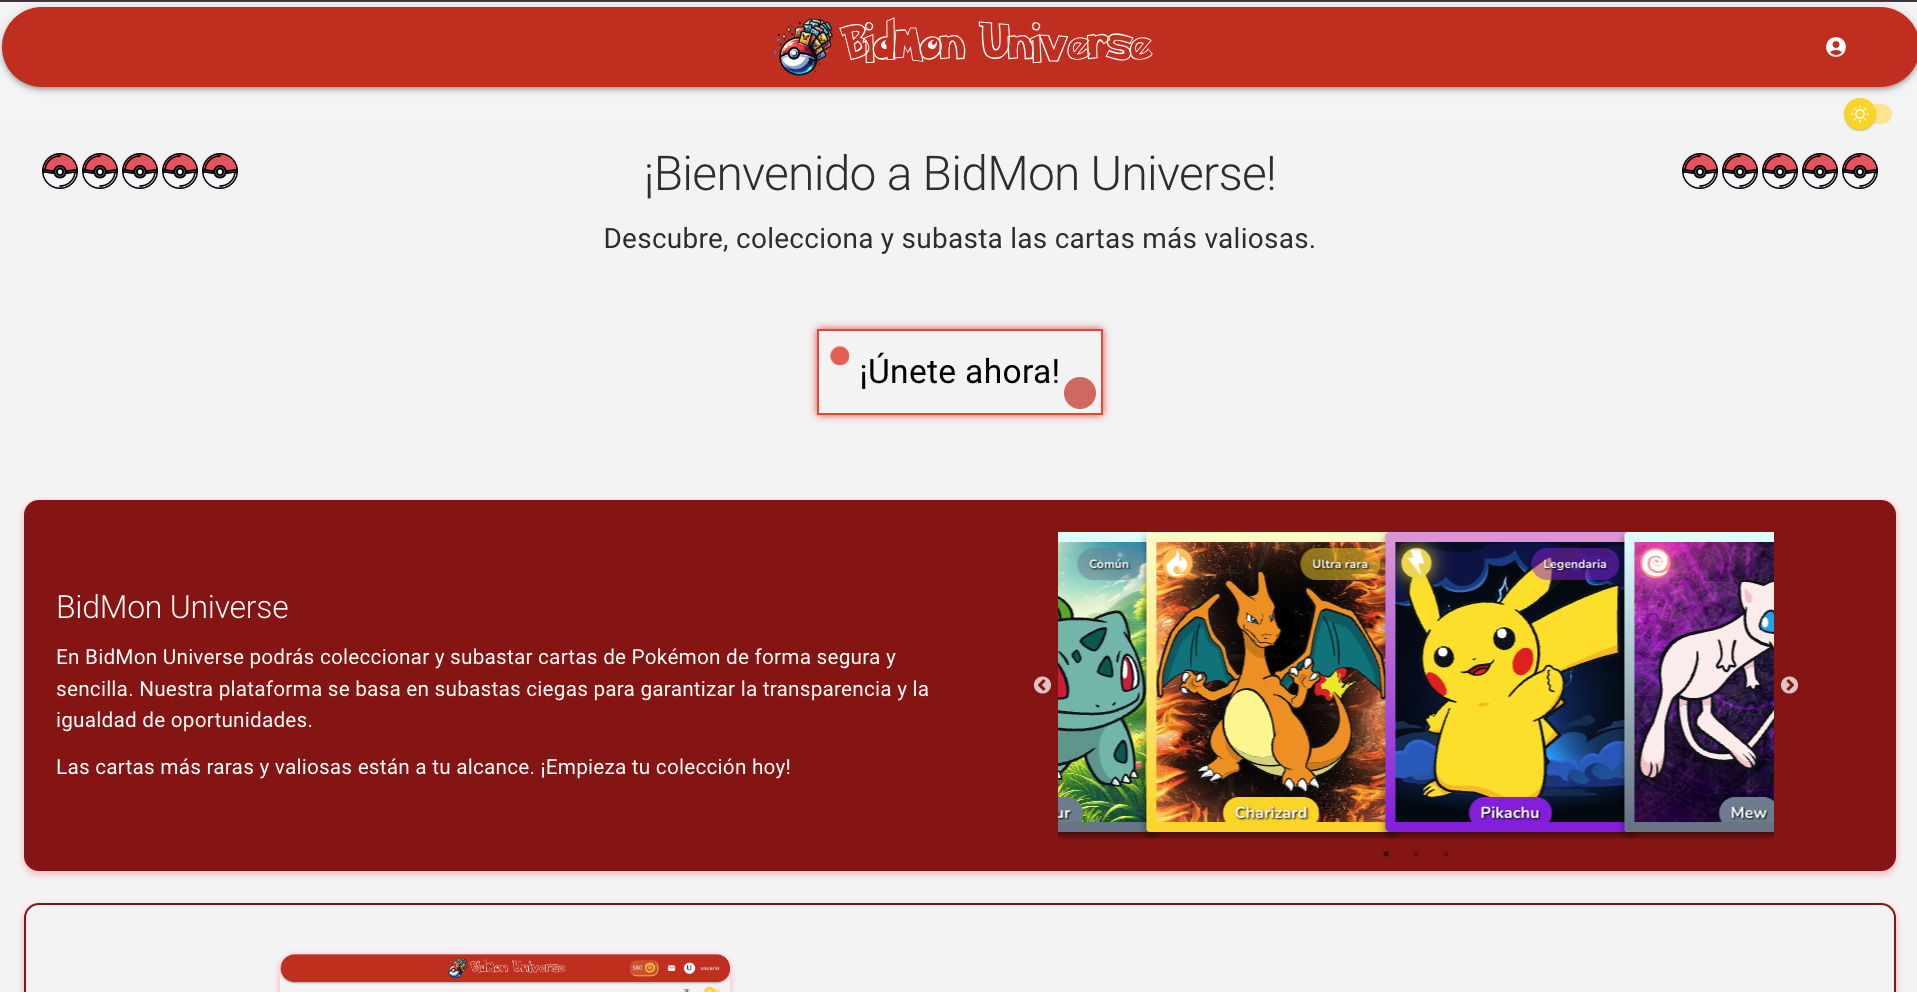
\includegraphics[width=0.8\textwidth]{figures/6-Analisis/6-Interfaz/interfaz/home.png}
    \caption{Página Home, página de inicio de la aplicación.}
    \label{fig:interfaz-home}
\end{figure}

\begin{figure}[H]
    \centering
    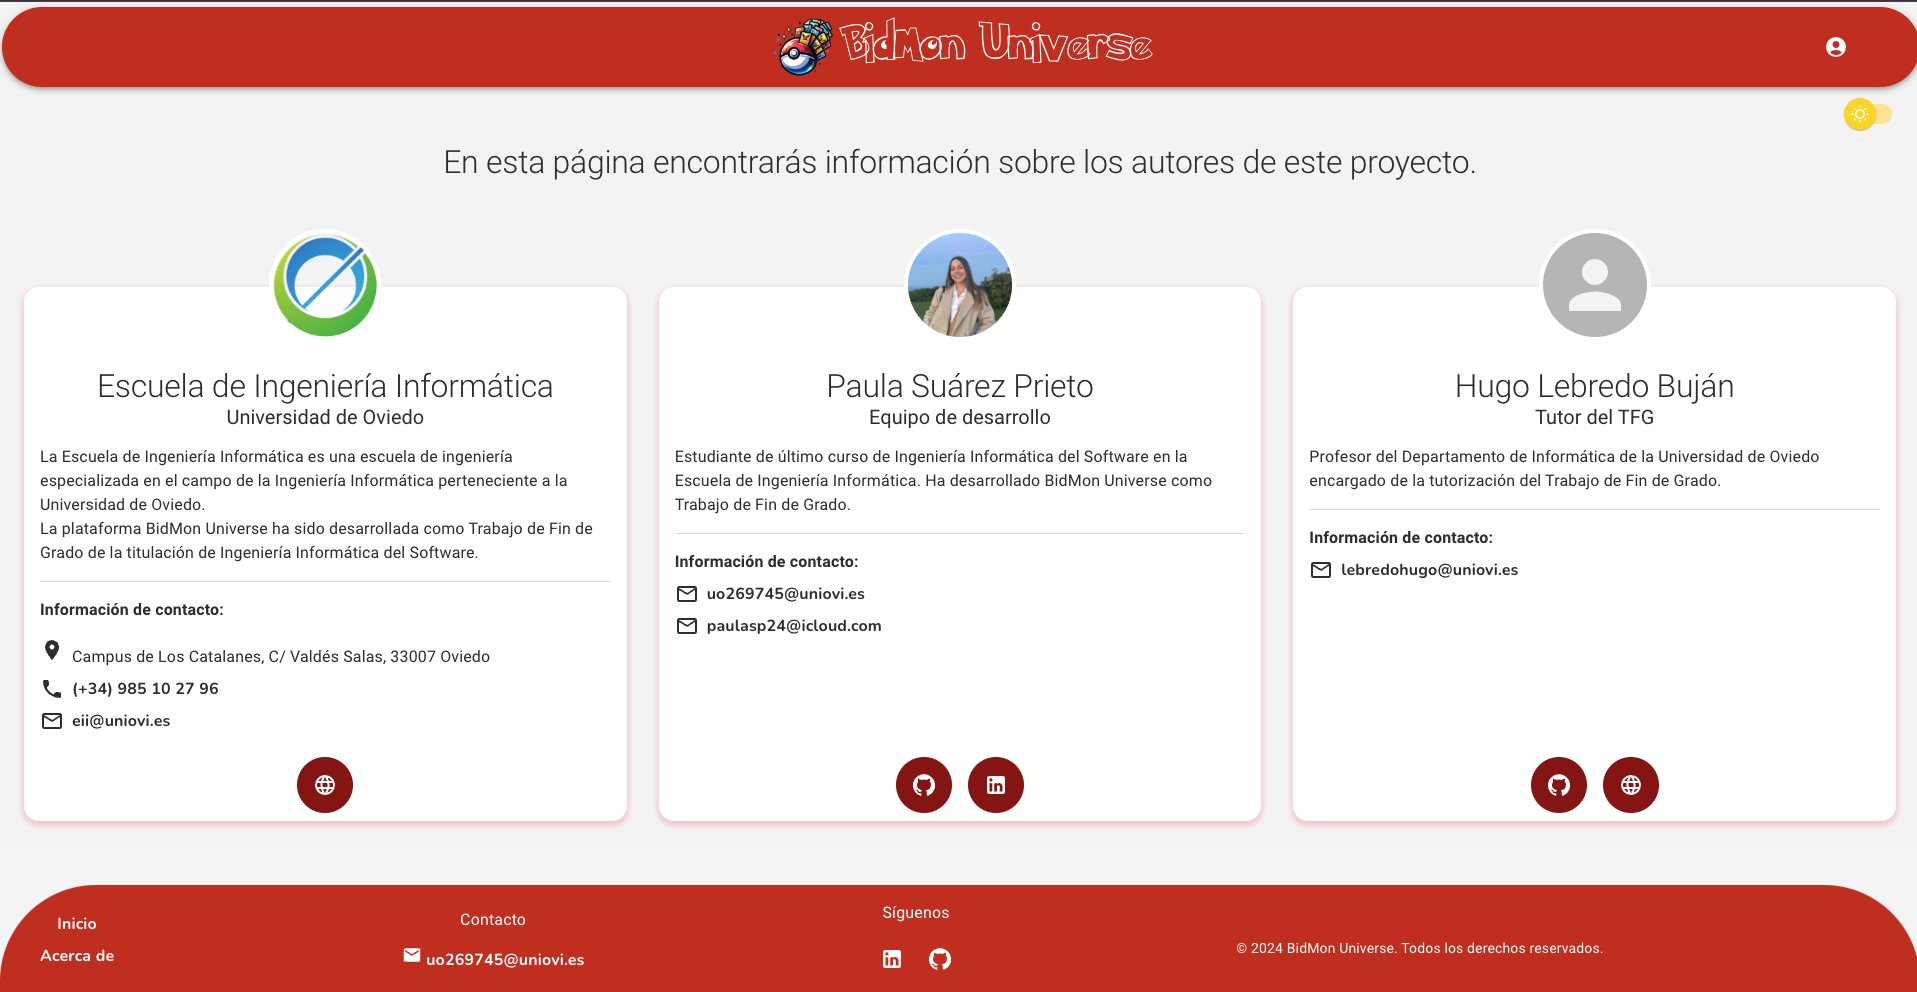
\includegraphics[width=0.8\textwidth]{figures/6-Analisis/6-Interfaz/interfaz/about.png}
    \caption{Página de información sobre la aplicación.}
    \label{fig:interfaz-about}
\end{figure}

\begin{figure}[H]
    \centering
    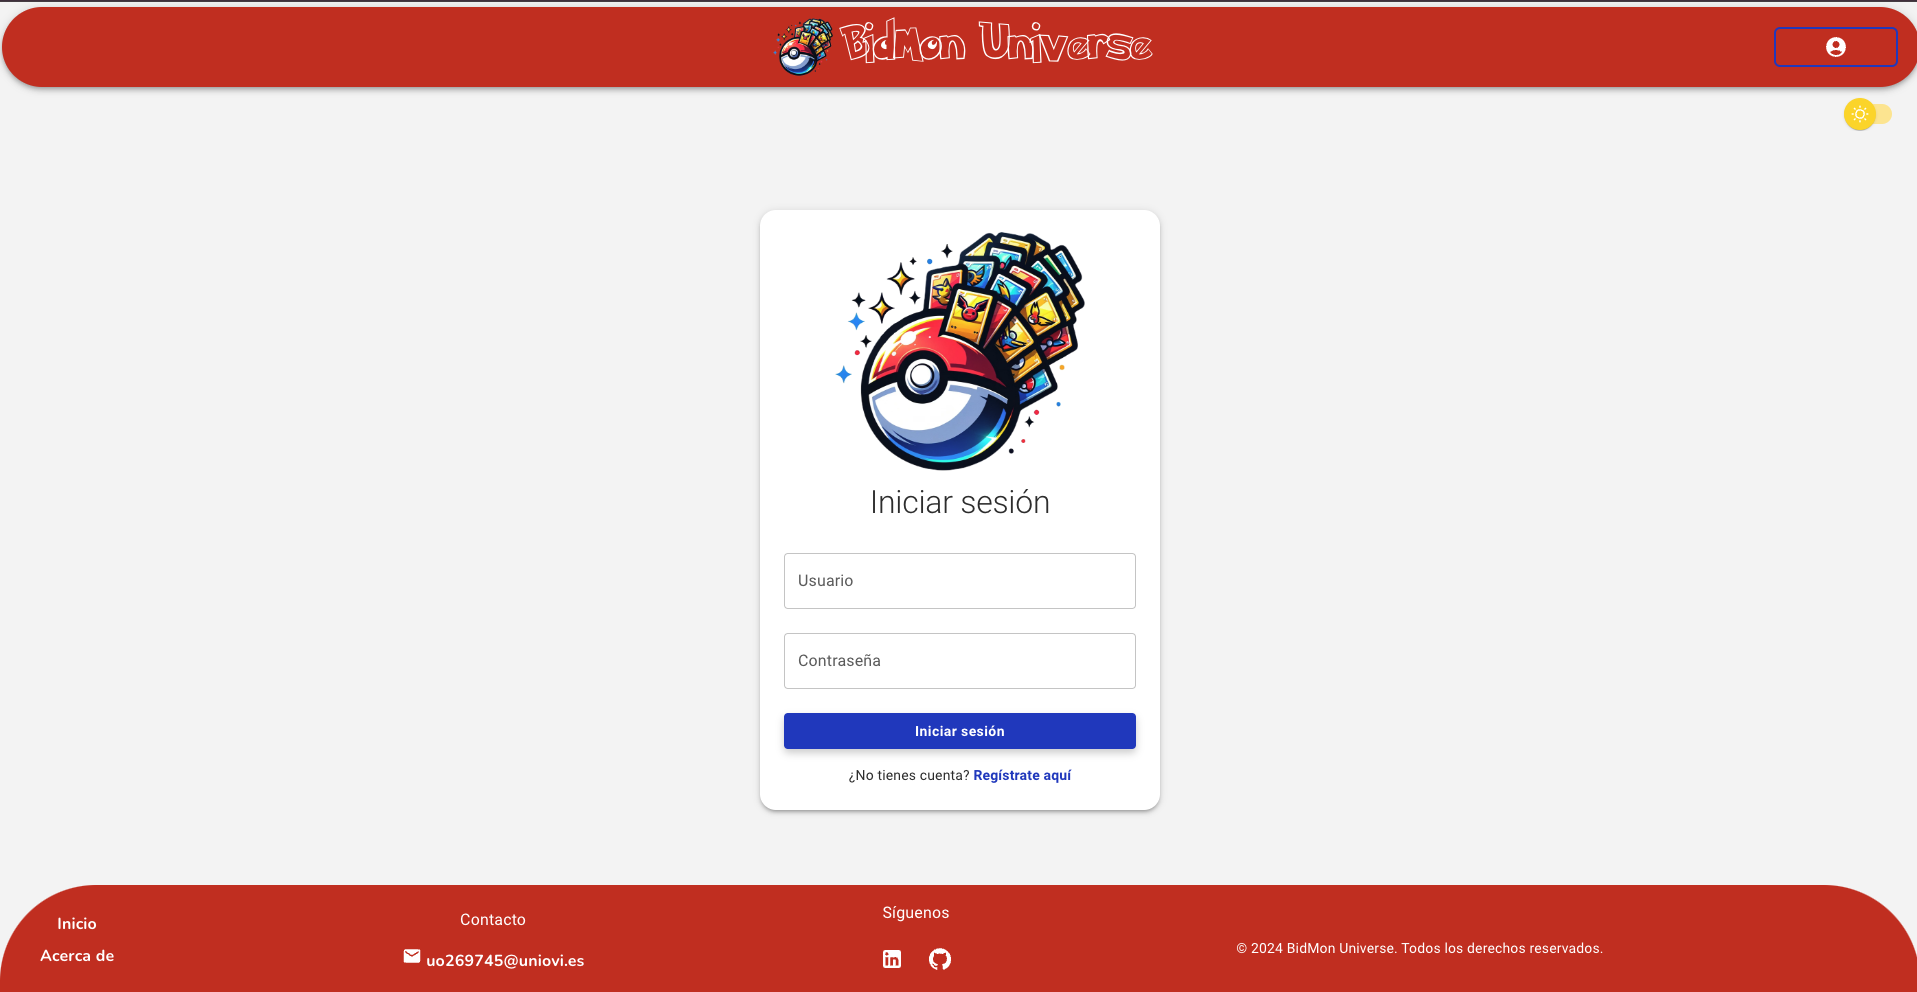
\includegraphics[width=0.8\textwidth]{figures/6-Analisis/6-Interfaz/interfaz/login.png}
    \caption{Página de inicio de sesión.}
    \label{fig:interfaz-login}
\end{figure}

\begin{figure}[H]
    \centering
    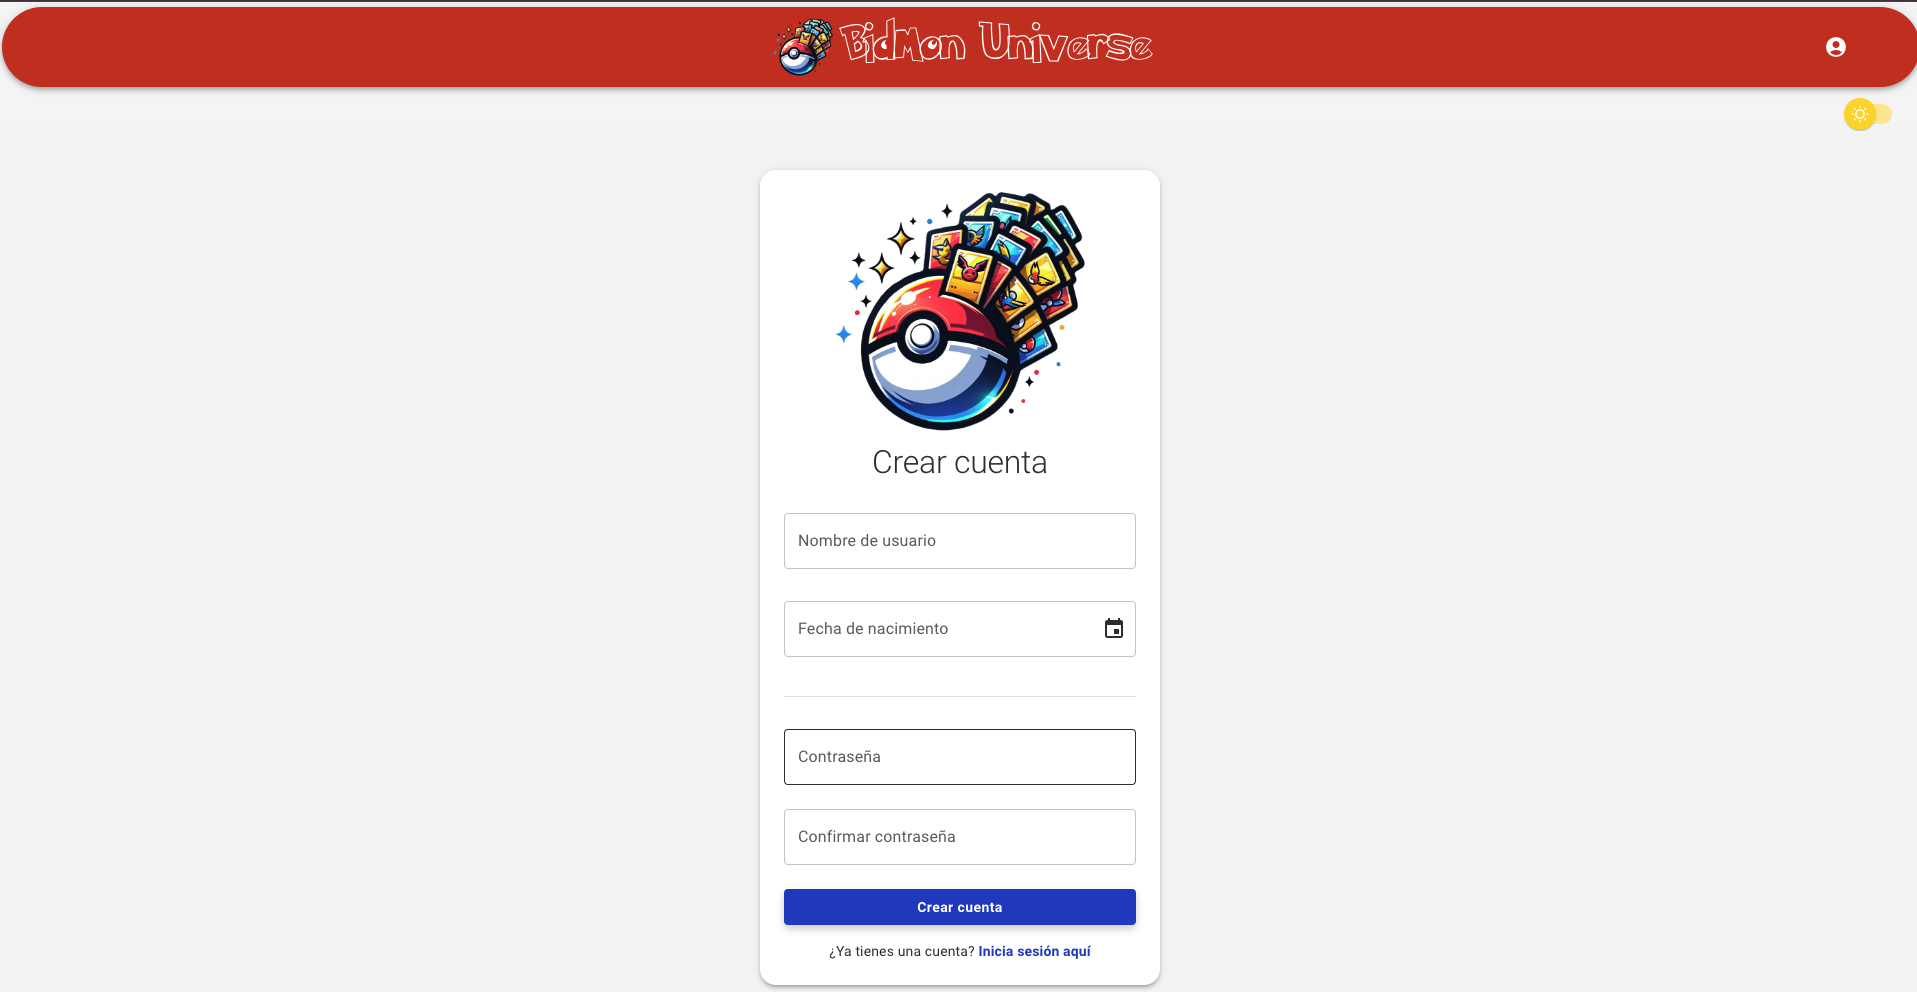
\includegraphics[width=0.8\textwidth]{figures/6-Analisis/6-Interfaz/interfaz/signup.png}
    \caption{Página de registro de usuario.}
    \label{fig:interfaz-registro}
\end{figure}

\begin{figure}[H]
    \centering
    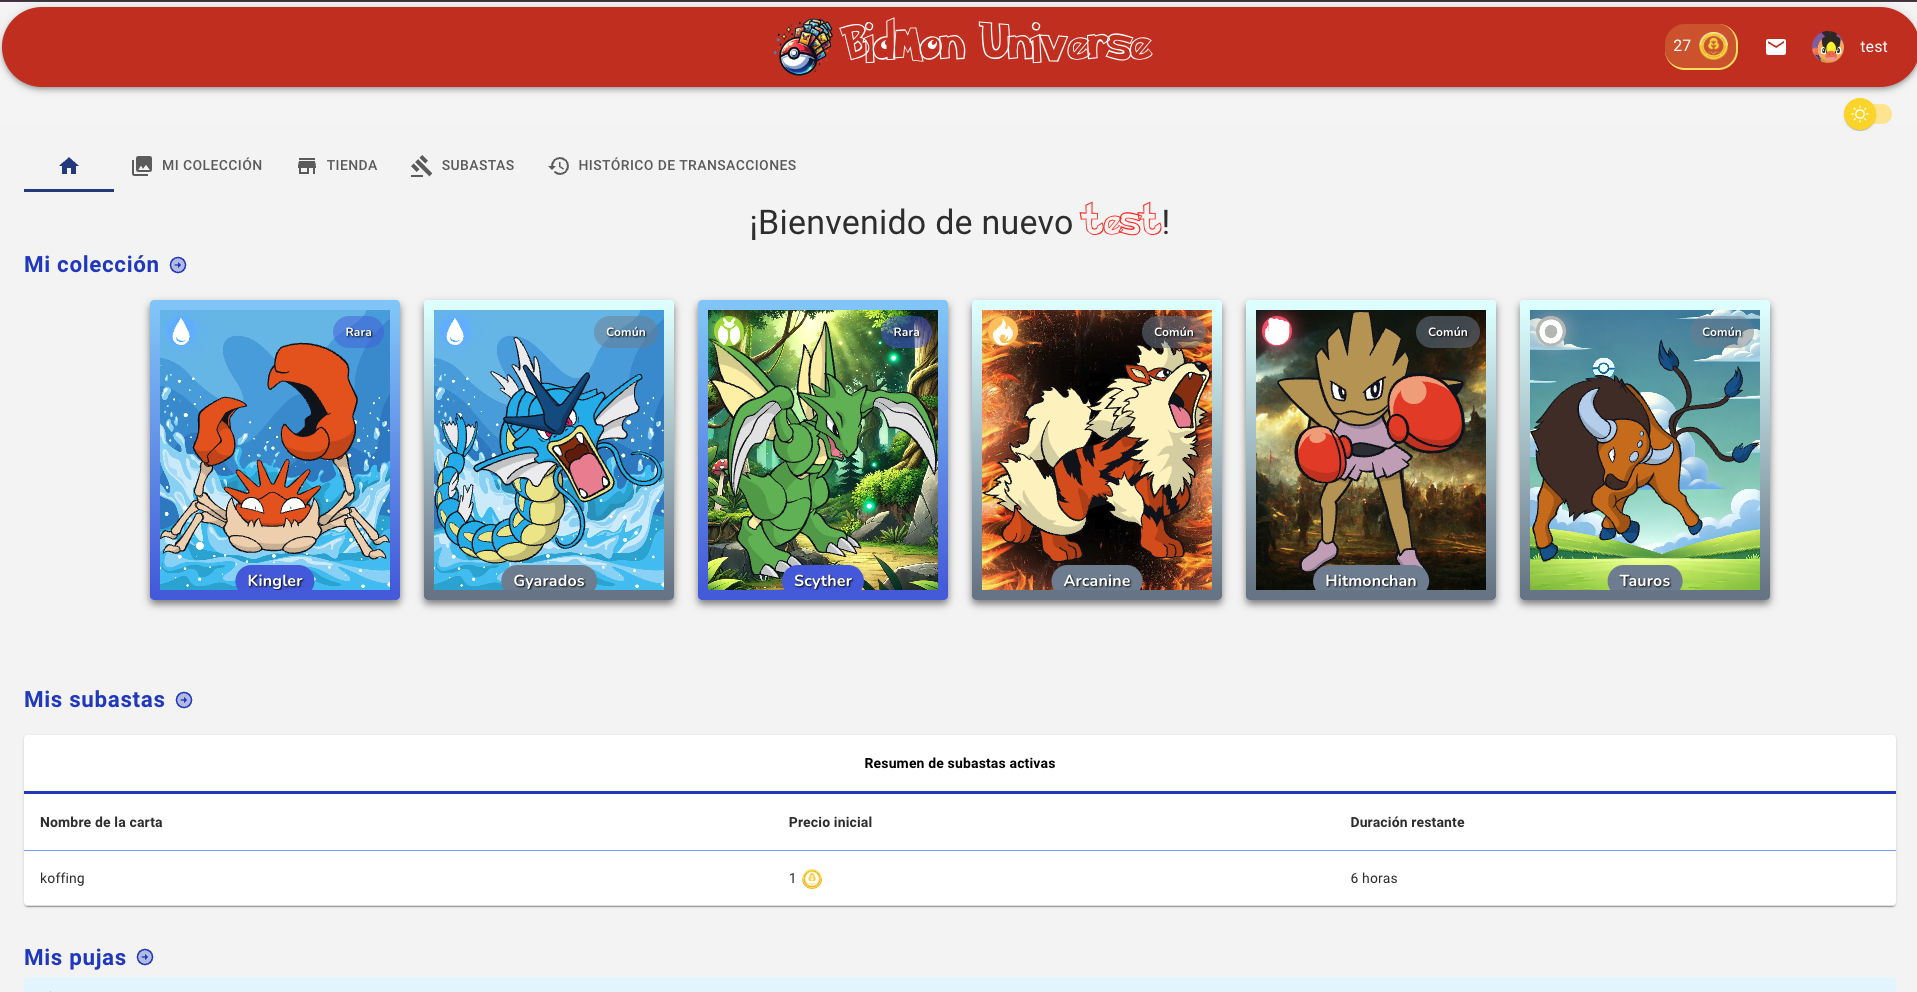
\includegraphics[width=0.8\textwidth]{figures/6-Analisis/6-Interfaz/interfaz/logued.png}
    \caption{Página principal de la aplicación, una vez que el usuario ha iniciado sesión.}
    \label{fig:interfaz-logued}
\end{figure}


\begin{figure}[H]
    \centering
    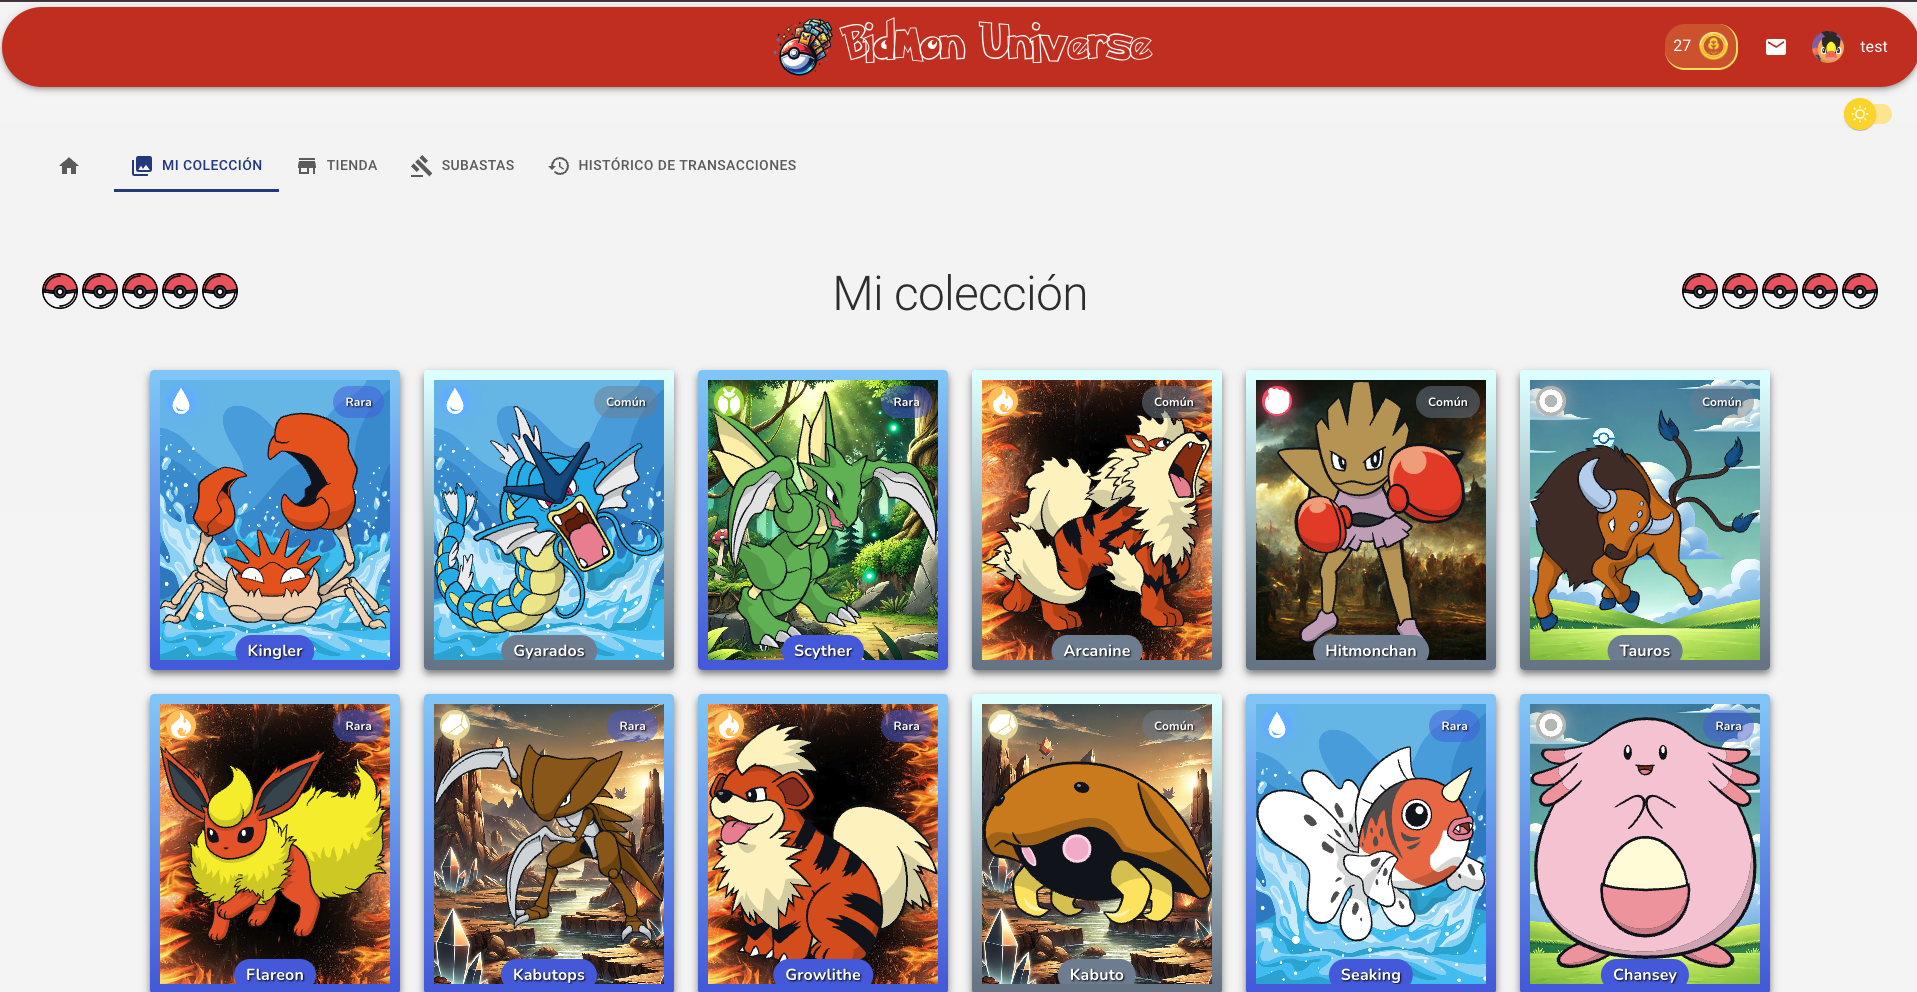
\includegraphics[width=0.8\textwidth]{figures/6-Analisis/6-Interfaz/interfaz/coleccion.png}
    \caption{Página de la colección de cartas del usuario.}
    \label{fig:interfaz-coleccion}
\end{figure}


\begin{figure}[H]
    \centering
    \includegraphics[width=0.8\textwidth]{figures/6-Analisis/6-Interfaz/interfaz/detalle_carta.png}
    \caption{Página de detalle de una carta de la colección del usuario.}
    \label{fig:interfaz-detalle-carta}
\end{figure}


\begin{figure}[H]
    \centering
    \includegraphics[width=0.8\textwidth]{figures/6-Analisis/6-Interfaz/interfaz/subastas.png}
    \caption{Página de las subastas activas de cartas.}
    \label{fig:interfaz-subastas}
\end{figure}


\begin{figure}[H]
    \centering
    \includegraphics[width=0.8\textwidth]{figures/6-Analisis/6-Interfaz/interfaz/detalle_subasta.png}
    \caption{Página de detalle de una subasta activa.}
    \label{fig:interfaz-detalle-subasta}
\end{figure}

\begin{figure}[H]
    \centering
    \includegraphics[width=0.8\textwidth]{figures/6-Analisis/6-Interfaz/interfaz/mi_subasta_detalle.png}
    \caption{Página de detalle de una subasta activa creada por el usuario.}
    \label{fig:interfaz-detalle-mi-subasta}
\end{figure}


\begin{figure}[H]
    \centering
    \includegraphics[width=0.8\textwidth]{figures/6-Analisis/6-Interfaz/interfaz/pujas.png}
    \caption{Página de pujas activas del usuario en subastas.}
    \label{fig:interfaz-gimnasios}
\end{figure}


\begin{figure}[H]
    \centering
    \includegraphics[width=0.8\textwidth]{figures/6-Analisis/6-Interfaz/interfaz/tienda.png}
    \caption{Página de la tienda de sobres de cartas.}
    \label{fig:interfaz-tienda}
\end{figure}


\begin{figure}[H]
    \centering
    \includegraphics[width=0.8\textwidth]{figures/6-Analisis/6-Interfaz/interfaz/recarga.png}
    \caption{Página de recarga de saldo de la aplicación.}
    \label{fig:interfaz-recarga}
\end{figure}


\begin{figure}[H]
    \centering
    \includegraphics[width=0.8\textwidth]{figures/6-Analisis/6-Interfaz/interfaz/transacciones.png}
    \caption{Página de transacciones realizadas por el usuario.}
    \label{fig:interfaz-transacciones}
\end{figure}

\begin{figure}[H]
    \centering
    \includegraphics[width=0.8\textwidth]{figures/6-Analisis/6-Interfaz/interfaz/perfil1.png}
    \caption{Página de perfil del usuario.}
    \label{fig:interfaz-perfil1}
\end{figure}


\begin{figure}[H]
    \centering
    \includegraphics[width=0.8\textwidth]{figures/6-Analisis/6-Interfaz/interfaz/perfil2.png}
    \caption{Página de perfil del usuario, con la opción de cambiar la imagen de perfil desplegada.}
    \label{fig:interfaz-perfil2}
\end{figure}


\begin{figure}[H]
    \centering
    \includegraphics[width=0.8\textwidth]{figures/6-Analisis/6-Interfaz/interfaz/notificaciones_2.png}
    \caption{Página de notificaciones del usuario.}
    \label{fig:interfaz-notificaciones}
\end{figure}


El usuario puede elegir entre dos temas de la aplicación: el tema claro y el tema oscuro.
El tema claro es el que se muestra en las imágenes anteriores.
A continuación se adjuntan un par de imágenes de la aplicación en el tema oscuro, la página de inicio
y la página de pujas activas del usuario.

\begin{figure}[H]
    \centering
    \includegraphics[width=0.8\textwidth]{figures/6-Analisis/6-Interfaz/interfaz/home_dark.png}
    \caption{Página Home en tema oscuro.}
    \label{fig:interfaz-home-dark}
\end{figure}

\begin{figure}[H]
    \centering
    \includegraphics[width=0.8\textwidth]{figures/6-Analisis/6-Interfaz/interfaz/pujas_dark.png}
    \caption{Página de pujas activas del usuario en tema oscuro.}
    \label{fig:interfaz-pujas-dark}
\end{figure}

\subsection{Descripción del Comportamiento de la Interfaz} 
La interacción con la interfaz es sencilla,
los botones tienen dos funcionalidades principales que son la de redirigir a otra página o la de realizar una acción.

Esta acción puede ser la de abrir un modal, como en el caso de la subasta de una carta o un menú desplegable, como en el caso del menú de usuario.

Los comportamientos más complejos de la interfaz son los de la subasta de una carta y la compra de un sobre de cartas.
Estos comportamientos se han diseñado de forma que sean intuitivos y fáciles de entender para el usuario.

A continuación, se mostrará un ejemplo de cada uno de estos comportamientos.

\subsubsection{Subasta de una carta}
En la \coloredUnderline{\hyperlink{fig:interfaz-subasta}{Figura \ref*{fig:interfaz-subasta}}} se muestra la vista del modal de crear una subasta.
En esta vista, el usuario puede seleccionar el precio de salida de la carta y el tiempo que durará la subasta.

\begin{figure}[H]
    \centering
    \includegraphics[width=0.8\textwidth]{figures/6-Analisis/6-Interfaz/interfaz/crear-subasta1.png}
    \caption{Modal de creación de subasta.}
    \hypertarget{fig:interfaz-subasta}{}
    \label{fig:interfaz-subasta}
\end{figure}

Una vez que el usuario ha rellenado los campos, puede pulsar el botón de \textit{Crear subasta} para confirmar la subasta.
Se le abrirá un modal de confirmación, en el que se le mostrará un resumen de la subasta y podrá confirmarla o cancelarla.

\begin{figure}[H]
    \centering
    \includegraphics[width=0.8\textwidth]{figures/6-Analisis/6-Interfaz/interfaz/crear-subasta2.png}
    \caption{Modal de confirmación de subasta.}
    \label{fig:interfaz-subasta-alerta}
\end{figure}

Si confirma la subasta, se mostrará un mensaje de éxito, se cerrará el modal y desparecerá el botón de subastar reemplazándolo por una
alerta informativa de que la carta está en subasta.

\begin{figure}[H]
    \centering
    \includegraphics[width=0.8\textwidth]{figures/6-Analisis/6-Interfaz/interfaz/subasta_creada.png}
    \caption{Mensaje de éxito de creación de subasta.}
    \label{fig:interfaz-subasta-exito}
\end{figure}

\begin{figure}[H]
    \centering
    \includegraphics[width=0.8\textwidth]{figures/6-Analisis/6-Interfaz/interfaz/subasta_creada2.png}
    \caption{Alerta de que la carta está en subasta.}
    \label{fig:interfaz-subasta-alerta}
\end{figure}

Si el usuario cancelase en algún momento el proceso de subasta, se cerraría el modal.


\subsubsection{Compra de un sobre de cartas}
El proceso de compra de un sobre de cartas es más sencillo que el de la subasta de una carta.
El usuario pulsa el botón de \textit{Comprar sobre} del sobre que desea comprar y se le abrirá un modal de confirmación.

\begin{figure}[H]
    \centering
    \includegraphics[width=0.8\textwidth]{figures/6-Analisis/6-Interfaz/interfaz/compra_sobre1.png}
    \caption{Modal de confirmación de compra de sobre.}
    \label{fig:interfaz-compra-sobre}
\end{figure}

Una vez que el usuario confirma la compra, se le mostrarán las cartas que ha obtenido en el sobre y un mensaje de éxito.
Estas cartas aparecen volteadas por lo que el usuario debe pulsar sobre ellas para verlas.
Tiene la opción de cerrar el modal o de ir a la colección de cartas para ver las cartas que ha obtenido.

\begin{figure}[H]
    \centering
    \includegraphics[width=0.8\textwidth]{figures/6-Analisis/6-Interfaz/interfaz/compra_sobre.png}
    \caption{Modal de cartas obtenidas en el sobre.}
    \label{fig:interfaz-sobre-comprado}
\end{figure}





\subsection{Diagrama de Navegabilidad}
En la sección \coloredUnderline{\hyperlink{sec:6_1-Identificacion_actores}{\ref*{sec:6_1-Identificacion_actores} \nameref*{sec:6_1-Identificacion_actores}}} se identificaron los actores del sistema,
cada uno con niveles de acceso y funcionalidades específicas adecuadas a su rol dentro de la plataforma. 

En este apartado se detalla el diagrama de navegabilidad de cada uno de los actores identificados en la sección mencionada anteriormente.
Para cada actor se detallan las vistas a las que puede acceder.

Las cajas que aparecen sombreadas en el diagrama representan las vistas que son accesibles desde cualquier otra vista,
debido a que se encuentran bien en el menú de navegación o en el pie de página de la aplicación.

La vista \textit{Home} es la vista principal de la aplicación, en función de si el usuario está autenticado o no, tendrá
una funcionalidad u otra, pero siempre es el punto de partida de la navegación y accesible desde cualquier vista.


\subsubsection{Usuario no autenticado}
En la \coloredUnderline{\hyperlink{fig:navegabilidad-usuario-no-autenticado}{Figura \ref*{fig:navegabilidad-usuario-no-autenticado}}} se muestra el diagrama de navegabilidad del usuario no autenticado.

\begin{figure}[H]
    \centering
    \includegraphics[width=0.5\textwidth]{figures/6-Analisis/6-Interfaz/navegabilidad-guest.png}
    \caption{Diagrama de navegabilidad del usuario no autenticado.}
    \hypertarget{fig:navegabilidad-usuario-no-autenticado}{}
    \label{fig:navegabilidad-usuario-no-autenticado}
\end{figure}

\subsubsection{Usuario autenticado}
En la \coloredUnderline{\hyperlink{fig:navegabilidad-usuario-autenticado}{Figura \ref*{fig:navegabilidad-usuario-autenticado}}} se muestra el diagrama de navegabilidad del usuario autenticado.

\begin{figure}[H]
    \centering
    \includegraphics[width=0.8\textwidth]{figures/6-Analisis/6-Interfaz/navegabilidad-standard.png}
    \caption{Diagrama de navegabilidad del usuario autenticado.}
    \hypertarget{fig:navegabilidad-usuario-autenticado}{}
    \label{fig:navegabilidad-usuario-autenticado}
\end{figure}

\subsubsection{Administrador}
En la \coloredUnderline{\hyperlink{fig:navegabilidad-administrador}{Figura \ref*{fig:navegabilidad-administrador}}} se muestra el diagrama de navegabilidad del administrador.

\begin{figure}[H]
    \centering
    \includegraphics[width=0.6\textwidth]{figures/6-Analisis/6-Interfaz/navegabilidad-admin.png}
    \caption{Diagrama de navegabilidad del administrador.}
    \hypertarget{fig:navegabilidad-administrador}{}
    \label{fig:navegabilidad-administrador}
\end{figure}



\newpage
\section{ESPECIFICACIÓN DEL PLAN DE PRUEBAS}
\subsection{Especificación del Plan de Pruebas}
Se realizarán cuatro tipos de pruebas para garantizar la calidad del sistema: pruebas unitarias, pruebas de integración, pruebas de usabilidad y pruebas de accesibilidad.
A continuación, se detallará cómo se llevarán a cabo las pruebas de cada tipo y se especificarán los criterios de aceptación para cada una de ellas.

\subsubsection{Pruebas Unitarias}
Las pruebas unitarias se realizarán para comprobar que cada componente del sistema funciona correctamente de forma aislada.
Se realizarán pruebas unitarias en el subsistema \textbf{restapi}, para comprobar que las rutas de la API REST funcionan correctamente, y en el subsistema \textbf{webapp}, para comprobar que los componentes de la interfaz de usuario se renderizan correctamente.

Para ello, se utilizará el framework de pruebas Jest para ambos subsistemas y se ejecutarán las pruebas en un entorno de test local.
Se espera que todas las pruebas unitarias pasen con éxito y que se alcance un porcentaje de cobertura de código mínima del 60\% para el subsistema \textbf{restapi} 
y para el subsistema \textbf{webapp} se deberán de cubrir los componentes que más se reutilizan en la aplicación.


Estas pruebas se realizarán en un entorno de test local, se utilizarán datos de prueba que simulan la información que se almacenará en la base de datos junto con una base de datos de pruebas.


\subsubsection{Pruebas de Integración}
Las pruebas de integración, también conocidas como pruebas de extremo a extremo o \textit{end-to-end}, se realizarán para comprobar que los distintos componentes del sistema funcionan correctamente en conjunto.
Se realizarán en el subsistema \textbf{webapp} con el framework de pruebas jest-cucumber y Puppeteer, que permite simular la interacción de un usuario con la aplicación y son muy descriptivas al iincluir escenarios de prueba escritos en lenguaje natural.
Estas pruebas se ejecutarán en un entorno de local de desarrollo y se utilizarán datos reales de la base de datos de desarrollo.

Los criterios de aceptación para estas pruebas son que se compruebe que un usuario puede iniciar sesión en la aplicación y que se renderice correctamente la página de inicio.

\subsubsection{Pruebas de Usabilidad}
Las pruebas de usabilidad se realizarán para comprobar que la interfaz de usuario es intuitiva y fácil de usar.
Se realizarán pruebas de usabilidad en el subsistema \textbf{webapp} con usuarios reales, que evaluarán la interfaz de usuario y proporcionarán retroalimentación sobre su usabilidad.
Estas pruebas se ejecutarán en un entorno de producción y se utilizarán datos reales de la base de datos de producción.
Los criterios de aceptación para estas pruebas son que no se reporten errores graves de usabilidad y que la interfaz de usuario sea fácil de usar para los usuarios reales.

\subsubsection{Pruebas de Accesibilidad}
Las pruebas de accesibilidad se realizarán para comprobar que la aplicación es accesible para personas con discapacidades.
Se utilizará el plugin de Google Chrome 
\coloredUnderline{\href{https://chromewebstore.google.com/detail/wave-evaluation-tool/jbbplnpkjmmeebjpijfedlgcdilocofh}{WAVE Evaluation Tool}} para comprobar la accesibilidad de la aplicación,
también se utilizará Google Lighthouse para comprobar la accesibilidad de la aplicación.

En un primer lugar se realizarán las pruebas de accesibilidad en el entorno de desarrollo y posteriormente, se repetirán en el entorno de producción con los errores corregidos.

Los criterios de aceptación para estas pruebas es que no haya errores de accesibilidad en el plugin WAVE Evaluation Tool,
permitiendo solo los errores de accesibilidad relacionados con el diseño específico de la aplicación.


\subsubsection{Pruebas de adaptabilidad}
Las pruebas de adaptabilidad se realizarán para comprobar que la aplicación se renderiza correctamente en distintos dispositivos y navegadores.
Las pruebas se realizarán en el entorno de producción y se utilizarán distintos dispositivos y navegadores para comprobar la adaptabilidad de la aplicación.
Los criterios de aceptación para estas pruebas son que la aplicación se renderice correctamente en dispositivos móviles, tabletas y ordenadores, y que funcione correctamente en los navegadores Google Chrome, Mozilla Firefox y Safari.


\subsection{Resultados de las Pruebas}
En esta sección se especificará en primer lugar las características del dispositivo y de los navegadores utilizados, y a continuación se detallarán los resultados de las pruebas realizadas.

\subsubsection{Dispositivo y navegadores utilizados}
Las pruebas se han llevado a cabo en un ordenador portátil con las siguientes características:
\begin{itemize}
    \item \textbf{Sistema Operativo}: macOS Sonoma 14.5.
    \item \textbf{Procesador}: Apple M3 Pro Max.
    \item \textbf{CPU}: 14 núcleos.
    \item \textbf{GPU}: 30 núcleos.
    \item \textbf{Memoria RAM}: 36 GB.
\end{itemize}

Como navegador se ha utilizado Google Chrome principalmente, las pruebas de adaptabilidad se han realizado además en Mozilla Firefox y Safari.
Las versiones de los navegadores son las siguientes:
\begin{itemize}
    \item \textbf{Google Chrome}: Versión 126.0.6478.127 (64 bits).
    \item \textbf{Mozilla Firefox}: Versión 127.0.2 (64 bits).
    \item \textbf{Safari}: Versión 17.5 (19618.2.12.11.6)
\end{itemize}


\subsubsection{Pruebas Unitarias}
Las pruebas unitarias se han realizado con éxito, se han comprobado que los componentes del sistema funcionan correctamente de forma aislada.
Se han realizado pruebas unitarias para cada \textit{router} del subsistema \textbf{restapi} y para los componentes más importantes del subsistema \textbf{webapp}. 

\subsubsubsection{Pruebas Unitarias. Restapi}
En el subsistema \textbf{restapi} se han realizado 51 pruebas unitarias, todas ellas han pasado con éxito obteniendo un 76.78\% de cobertura de código para \textit{routers}.
Se puede ver detallado el porcentaje de cobertura de código en la \coloredUnderline{\hyperlink{fig:6_8_Cobertura-Code-Restapi}{Figura \ref*{fig:6_8_Cobertura-Code-Restapi}: \nameref*{fig:6_8_Cobertura-Code-Restapi}}}.
\begin{figure}[H]
    \hypertarget{fig:6_8_Cobertura-Code-Restapi}{}
    \centering
    \includegraphics[width=0.8\linewidth]{figures/6-Analisis/6-Pruebas/6_8-Coverage-Restapi.png}
    \caption{Cobertura de Código del Subsistema restapi}
    \label{fig:6_8_Cobertura-Code-Restapi}
\end{figure}

A continuación, se detallan las pruebas unitarias realizadas en el subsistema \textbf{restapi}, con su descripición y resultado esperado.
Cabe destacar que para la ejecución de todas las pruebas, salvo para \textit{POST /api/users/login} y \textit{POST /api/users/signup}, se ha utilizado un token de autenticación válido, 
es decir, se ha iniciado sesión previamente con un usuario existente.


%-------------------TABLA PRUEBAS UNITARIAS RESTAPI-------------------

%-------------------TESTS DE AUCTIONROUTER-------------------
\begin{longtable}{
    >{\columncolor{lightgreen!20}}p{4cm}
    p{6cm}
    p{4cm}
    }
    \caption{Tests de auctionRouter} \label{table:test_auctionRouter} \\
    \toprule
    \rowcolor{darkgreen!50}
    \multicolumn{3}{|c|}{\textbf{Tests de auctionRouter}}\\
    \midrule
    \rowcolor{darkgreen!30}
    \textbf{Ruta a probar} & \multicolumn{1}{>{\columncolor{darkgreen!50}\centering\arraybackslash}p{6cm}}{\textbf{Descripción}} & \multicolumn{1}{>{\columncolor{darkgreen!50}\centering\arraybackslash}p{4cm}}{\textbf{Resultado esperado}} \\
    \endfirsthead
    
    \multicolumn{3}{c}%
    {{ \tablename\ \thetable{} Tests de auctionRouter -- continuación de la página anterior}} \\
    \toprule
    \rowcolor{darkgreen!50}
    \multicolumn{3}{|c|}{\textbf{Tests de auctionRouter}}\\
    \midrule
    \rowcolor{darkgreen!30}
    \textbf{Ruta a probar} & \multicolumn{1}{>{\columncolor{darkgreen!50}\centering\arraybackslash}p{6cm}}{\textbf{Descripción}} & \multicolumn{1}{>{\columncolor{darkgreen!50}\centering\arraybackslash}p{4cm}}{\textbf{Resultado esperado}} \\
    \midrule
    \endhead
    
    \midrule
    \multicolumn{3}{r}{{Continúa en la siguiente página...}} \\ 
    \endfoot
    
    \bottomrule
    \endlastfoot
    
    \midrule
    \textbf{GET /api/auctions} & Devuelve todas las subastas. & 200, la respuesta contiene una lista de subastas. \\
    \midrule
    \textbf{GET /api/auctions/a/:id} & Devuelve una subasta específica. & 200, la respuesta contiene los datos de la subasta. \\
    \midrule
    \textbf{GET /api/auctions/a/:id (no existe)} & Devuelve 404 si el ID de la subasta no se encuentra. & 404, la respuesta indica que la subasta no se encuentra. \\
    \midrule
    \textbf{GET /api/auctions/active/:username} & Devuelve todas las subastas activas para un nombre de usuario válido. & 200, la respuesta contiene una lista de subastas activas. \\
    \midrule
    \textbf{GET /api/auctions/active/u/:username} & Devuelve todas las subastas activas para un usuario. & 200, la respuesta contiene una lista de subastas activas. \\
    \end{longtable}

%-------------------TESTS DE BIDROUTER-------------------
\begin{longtable}{
    >{\columncolor{lightgreen!20}}p{4cm}
    p{6cm}
    p{4cm}
    }
    \caption{Tests de bidRouter} \label{table:test_bidRouter} \\
    \toprule
    \rowcolor{darkgreen!50}
    \multicolumn{3}{|c|}{\textbf{Tests de bidRouter}}\\
    \midrule
    \rowcolor{darkgreen!30}
    \textbf{Ruta a probar} & \multicolumn{1}{>{\columncolor{darkgreen!50}\centering\arraybackslash}p{6cm}}{\textbf{Descripción}} & \multicolumn{1}{>{\columncolor{darkgreen!50}\centering\arraybackslash}p{4cm}}{\textbf{Resultado esperado}} \\
    \endfirsthead
    
    \multicolumn{3}{c}%
    {{ \tablename\ \thetable{} Tests de bidRouter -- continuación de la página anterior}} \\
    \toprule
    \rowcolor{darkgreen!50}
    \multicolumn{3}{|c|}{\textbf{Tests de bidRouter}}\\
    \midrule
    \rowcolor{darkgreen!30}
    \textbf{Ruta a probar} & \multicolumn{1}{>{\columncolor{darkgreen!50}\centering\arraybackslash}p{6cm}}{\textbf{Descripción}} & \multicolumn{1}{>{\columncolor{darkgreen!50}\centering\arraybackslash}p{4cm}}{\textbf{Resultado esperado}} \\
    \midrule
    \endhead
    
    \midrule
    \multicolumn{3}{r}{{Continúa en la siguiente página...}} \\ 
    \endfoot
    
    \bottomrule
    \endlastfoot
    
    \midrule
    \textbf{GET /api/bids/b/:id} & Devuelve una oferta específica. & 200, la respuesta contiene los datos de la oferta. \\
    \midrule
    \textbf{GET /api/bids/b/:id (no existe)} & Devuelve 404 si el ID de la oferta no se encuentra. & 404, la respuesta indica que la oferta no se encuentra. \\
    \midrule
    \textbf{GET /api/bids/active/u/:username} & Devuelve todas las ofertas activas para un nombre de usuario válido. & 200, la respuesta contiene una lista de ofertas activas. \\
    \end{longtable}

%-------------------TESTS DE CARDPACKROUTER-------------------
\begin{longtable}{
    >{\columncolor{lightgreen!20}}p{4cm}
    p{6cm}
    p{4cm}
    }
    \caption{Tests de cardPackRouter} \label{table:test_cardPackRouter} \\
    \toprule
    \rowcolor{darkgreen!50}
    \multicolumn{3}{|c|}{\textbf{Tests de cardPackRouter}}\\
    \midrule
    \rowcolor{darkgreen!30}
    \textbf{Ruta a probar} & \multicolumn{1}{>{\columncolor{darkgreen!50}\centering\arraybackslash}p{6cm}}{\textbf{Descripción}} & \multicolumn{1}{>{\columncolor{darkgreen!50}\centering\arraybackslash}p{4cm}}{\textbf{Resultado esperado}} \\
    \endfirsthead
    
    \multicolumn{3}{c}%
    {{ \tablename\ \thetable{} Tests de cardPackRouter -- continuación de la página anterior}} \\
    \toprule
    \rowcolor{darkgreen!50}
    \multicolumn{3}{|c|}{\textbf{Tests de cardPackRouter}}\\
    \midrule
    \rowcolor{darkgreen!30}
    \textbf{Ruta a probar} & \multicolumn{1}{>{\columncolor{darkgreen!50}\centering\arraybackslash}p{6cm}}{\textbf{Descripción}} & \multicolumn{1}{>{\columncolor{darkgreen!50}\centering\arraybackslash}p{4cm}}{\textbf{Resultado esperado}} \\
    \midrule
    \endhead
    
    \midrule
    \multicolumn{3}{r}{{Continúa en la siguiente página...}} \\ 
    \endfoot
    
    \bottomrule
    \endlastfoot
    
    \midrule
    \textbf{GET /api/cardpacks} & Devuelve todos los paquetes de cartas disponibles. & 200, la respuesta contiene una lista de paquetes de cartas filtrados por disponibilidad. \\
    \end{longtable}

%-------------------TESTS DE CARDROUTER-------------------
\begin{longtable}{
    >{\columncolor{lightgreen!20}}p{4cm}
    p{6cm}
    p{4cm}
    }
    \caption{Tests de cardRouter} \label{table:test_cardRouter} \\
    \toprule
    \rowcolor{darkgreen!50}
    \multicolumn{3}{|c|}{\textbf{Tests de cardRouter}}\\
    \midrule
    \rowcolor{darkgreen!30}
    \textbf{Ruta a probar} & \multicolumn{1}{>{\columncolor{darkgreen!50}\centering\arraybackslash}p{6cm}}{\textbf{Descripción}} & \multicolumn{1}{>{\columncolor{darkgreen!50}\centering\arraybackslash}p{4cm}}{\textbf{Resultado esperado}} \\
    \endfirsthead
    
    \multicolumn{3}{c}%
    {{ \tablename\ \thetable{} Tests de cardRouter -- continuación de la página anterior}} \\
    \toprule
    \rowcolor{darkgreen!50}
    \multicolumn{3}{|c|}{\textbf{Tests de cardRouter}}\\
    \midrule
    \rowcolor{darkgreen!30}
    \textbf{Ruta a probar} & \multicolumn{1}{>{\columncolor{darkgreen!50}\centering\arraybackslash}p{6cm}}{\textbf{Descripción}} & \multicolumn{1}{>{\columncolor{darkgreen!50}\centering\arraybackslash}p{4cm}}{\textbf{Resultado esperado}} \\
    \midrule
    \endhead
    
    \midrule
    \multicolumn{3}{r}{{Continúa en la siguiente página...}} \\ 
    \endfoot
    
    \bottomrule
    \endlastfoot
    
    \midrule
    \textbf{GET /api/cards/:cardId} & Devuelve una carta por su ID. & 200, la respuesta contiene los datos de la carta, incluyendo el nombre 'bulbasaur'. \\
    \midrule
    \textbf{GET /api/cards/:cardId (no existe)} & Devuelve 404 si la carta no se encuentra. & 404, la respuesta contiene el mensaje 'Carta no encontrada.'. \\
    \midrule
    \textbf{GET /api/cards/:cardId (error)} & Maneja errores de forma adecuada. & 500, la respuesta contiene el mensaje 'Se ha producido un error al obtener la carta.'. \\
    \end{longtable}



%-------------------TESTS DE DECKROUTER-------------------

\begin{longtable}{
    >{\columncolor{lightgreen!20}}p{4cm}
    p{6cm}
    p{4cm}
    }
    \caption{Tests de deckRouter} \label{table:test_deckRouter} \\
    \toprule
    \rowcolor{darkgreen!50}
    \multicolumn{3}{|c|}{\textbf{Tests de deckRouter}}\\
    \midrule
    \rowcolor{darkgreen!30}
    \textbf{Ruta a probar} & \multicolumn{1}{>{\columncolor{darkgreen!50}\centering\arraybackslash}p{6cm}}{\textbf{Descripción}} & \multicolumn{1}{>{\columncolor{darkgreen!50}\centering\arraybackslash}p{4cm}}{\textbf{Resultado esperado}} \\
    \endfirsthead
    
    \multicolumn{3}{c}%
    {{ \tablename\ \thetable{} Tests de deckRouter -- continuación de la página anterior}} \\
    \toprule
    \rowcolor{darkgreen!50}
    \multicolumn{3}{|c|}{\textbf{Tests de deckRouter}}\\
    \midrule
    \rowcolor{darkgreen!30}
    \textbf{Ruta a probar} & \multicolumn{1}{>{\columncolor{darkgreen!50}\centering\arraybackslash}p{6cm}}{\textbf{Descripción}} & \multicolumn{1}{>{\columncolor{darkgreen!50}\centering\arraybackslash}p{4cm}}{\textbf{Resultado esperado}} \\
    \midrule
    \endhead
    
    \midrule
    \multicolumn{3}{r}{{Continúa en la siguiente página...}} \\ 
    \endfoot
    
    \bottomrule
    \endlastfoot
    
    \midrule
    \textbf{GET /api/decks} & Devuelve todos los mazos de cartas. & 200, la respuesta contiene una lista de mazos de cartas. \\
    \midrule
    \textbf{GET /api/decks/:deckid} & Devuelve un mazo de cartas por su ID. & 200, la respuesta contiene los datos del mazo de cartas, incluyendo 'deckId', 'name', 'type', y 'publicationDate'. \\
    \midrule
    \textbf{GET /api/decks (error)} & Maneja errores de forma adecuada al obtener todos los mazos de cartas. & 500, la respuesta contiene el mensaje 'Se ha producido un error al obtener los mazos de cartas.'. \\
    \midrule
    \textbf{GET /api/decks/:deckid (no existe)} & Devuelve 404 si el mazo de cartas no se encuentra. & 404, la respuesta contiene el mensaje 'Mazo de cartas no encontrado.'. \\
    \midrule
    \textbf{GET /api/decks/:deckid (error)} & Maneja errores de forma adecuada al obtener un mazo de cartas por su ID. & 500, la respuesta contiene el mensaje 'Se ha producido un error al obtener el mazo de cartas.'. \\
    \end{longtable}


%-------------------TESTS DE NOTIFICATIONROUTER-------------------
\begin{longtable}{
    >{\columncolor{lightgreen!20}}p{4cm}
    p{6cm}
    p{4cm}
    }
    \caption{Tests de notificationRouter} \label{table:test_notificationRouter} \\
    \toprule
    \rowcolor{darkgreen!50}
    \multicolumn{3}{|c|}{\textbf{Tests de notificationRouter}}\\
    \midrule
    \rowcolor{darkgreen!30}
    \textbf{Ruta a probar} & \multicolumn{1}{>{\columncolor{darkgreen!50}\centering\arraybackslash}p{6cm}}{\textbf{Descripción}} & \multicolumn{1}{>{\columncolor{darkgreen!50}\centering\arraybackslash}p{4cm}}{\textbf{Resultado esperado}} \\
    \endfirsthead
    
    \multicolumn{3}{c}%
    {{ \tablename\ \thetable{} Tests de notificationRouter -- continuación de la página anterior}} \\
    \toprule
    \rowcolor{darkgreen!50}
    \multicolumn{3}{|c|}{\textbf{Tests de notificationRouter}}\\
    \midrule
    \rowcolor{darkgreen!30}
    \textbf{Ruta a probar} & \multicolumn{1}{>{\columncolor{darkgreen!50}\centering\arraybackslash}p{6cm}}{\textbf{Descripción}} & \multicolumn{1}{>{\columncolor{darkgreen!50}\centering\arraybackslash}p{4cm}}{\textbf{Resultado esperado}} \\
    \midrule
    \endhead
    
    \midrule
    \multicolumn{3}{r}{{Continúa en la siguiente página...}} \\ 
    \endfoot
    
    \bottomrule
    \endlastfoot
    
    \midrule
    \textbf{GET /api/notifications/:username} & Devuelve todas las notificaciones para un nombre de usuario válido. & 200, la respuesta contiene una lista de notificaciones. \\
    \midrule
    \textbf{GET /api/notifications/unread/:username} & Devuelve todas las notificaciones no leídas para un nombre de usuario válido. & 200, la respuesta contiene una lista de notificaciones no leídas. \\
    \midrule
    \textbf{PATCH /api/notifications/notification/:notificationId/read} & Marca una notificación como leída. & 200, la respuesta indica éxito. \\
    \midrule
    \textbf{PATCH /api/notifications/read/:username} & Marca todas las notificaciones de un usuario como leídas. & 200, la respuesta indica éxito. \\
    \end{longtable}


%-------------------TESTS DE PURCHASESROUTER-------------------
\begin{longtable}{
    >{\columncolor{lightgreen!20}}p{4cm}
    p{6cm}
    p{4cm}
    }
    \caption{Tests de purchasesRouter} \label{table:test_purchasesRouter} \\
    \toprule
    \rowcolor{darkgreen!50}
    \multicolumn{3}{|c|}{\textbf{Tests de purchasesRouter}}\\
    \midrule
    \rowcolor{darkgreen!30}
    \textbf{Ruta a probar} & \multicolumn{1}{>{\columncolor{darkgreen!50}\centering\arraybackslash}p{6cm}}{\textbf{Descripción}} & \multicolumn{1}{>{\columncolor{darkgreen!50}\centering\arraybackslash}p{4cm}}{\textbf{Resultado esperado}} \\
    \endfirsthead
    
    \multicolumn{3}{c}%
    {{ \tablename\ \thetable{} Tests de purchasesRouter -- continuación de la página anterior}} \\
    \toprule
    \rowcolor{darkgreen!50}
    \multicolumn{3}{|c|}{\textbf{Tests de purchasesRouter}}\\
    \midrule
    \rowcolor{darkgreen!30}
    \textbf{Ruta a probar} & \multicolumn{1}{>{\columncolor{darkgreen!50}\centering\arraybackslash}p{6cm}}{\textbf{Descripción}} & \multicolumn{1}{>{\columncolor{darkgreen!50}\centering\arraybackslash}p{4cm}}{\textbf{Resultado esperado}} \\
    \midrule
    \endhead
    
    \midrule
    \multicolumn{3}{r}{{Continúa en la siguiente página...}} \\ 
    \endfoot
    
    \bottomrule
    \endlastfoot
    
    \midrule
    \textbf{POST /api/purchases/cardpack} & Compra un paquete de cartas exitosamente, disminuyendo la cantidad disponible del paquete y el saldo del usuario, creando cartas de usuario y transacciones. & 200, la respuesta indica éxito y las verificaciones post-compra son correctas. \\
    \midrule
    \textbf{POST /api/purchases/cardpack (usuario no existe)} & Maneja errores cuando el usuario no existe. & 500, la respuesta contiene el mensaje 'El usuario no existe.'. \\
    \midrule
    \textbf{POST /api/purchases/cardpack (saldo insuficiente)} & Maneja errores cuando el usuario no tiene suficiente saldo. & 500, la respuesta indica un error de saldo insuficiente. \\
    \midrule
    \textbf{POST /api/purchases/cardpack (paquete no existe)} & Maneja errores cuando el paquete de cartas no existe. & 500, la respuesta indica que el paquete de cartas no se encuentra. \\
    \midrule
    \textbf{POST /api/purchases/cardpack (paquete no disponible)} & Maneja errores cuando el paquete de cartas no está disponible. & 500, la respuesta indica que el paquete de cartas no está disponible. \\
    \end{longtable}



%-------------------TESTS DE TRANSACTIONROUTER-------------------
\begin{longtable}{
    >{\columncolor{lightgreen!20}}p{4cm}
    p{6cm}
    p{4cm}
    }
    \caption{Tests de transactionRouter} \label{table:descripcion_transactionRouter} \\
    \toprule
    \rowcolor{darkgreen!50}
    \multicolumn{3}{|c|}{\textbf{Tests de transactionRouter}}\\
    \midrule
    \rowcolor{darkgreen!30}
    \textbf{Ruta a probar} & \multicolumn{1}{>{\columncolor{darkgreen!50}\centering\arraybackslash}p{6cm}}{\textbf{Descripción}} & \multicolumn{1}{>{\columncolor{darkgreen!50}\centering\arraybackslash}p{4cm}}{\textbf{Resultado esperado}} \\
    \endfirsthead
    
    \multicolumn{3}{c}%
    {{ \tablename\ \thetable{} Tests de transactionRouter -- continuación de la página anterior}} \\
    \toprule
    \rowcolor{darkgreen!50}
    \multicolumn{3}{|c|}{\textbf{Tests de transactionRouter}}\\
    \midrule
    \rowcolor{darkgreen!30}
    \textbf{Ruta a probar} & \multicolumn{1}{>{\columncolor{darkgreen!50}\centering\arraybackslash}p{6cm}}{\textbf{Descripción}} & \multicolumn{1}{>{\columncolor{darkgreen!50}\centering\arraybackslash}p{4cm}}{\textbf{Resultado esperado}} \\
    \midrule
    \endhead
    
    \midrule
    \multicolumn{3}{r}{{Continúa en la siguiente página...}} \\ 
    \endfoot
    
    \bottomrule
    \endlastfoot
    
    \midrule
    \textbf{GET /api/transactions} & Devuelve todas las transacciones. & 200, la respuesta contiene una lista de transacciones. \\
    \midrule
    \textbf{GET /api/transactions/u/:username} & Devuelve las transacciones para un nombre de usuario válido. & 200, la respuesta contiene una lista de transacciones para el usuario. \\
    \midrule
    \textbf{GET /api/transactions/c/:userCardId} & Devuelve las transacciones para un ID de carta de usuario válido. & 200, la respuesta contiene una lista de transacciones para la carta de usuario. \\
    \midrule
    \textbf{GET /api/transactions (no admin)} & Devuelve 403 si el usuario no es administrador. & 403, la respuesta contiene el mensaje 'Acceso denegado. Se requiere rol de administrador.'. \\
    \midrule
    \textbf{GET /api/transactions/u/:username (username inválido)} & Devuelve 400 para un nombre de usuario inválido. & 400, la respuesta contiene errores de validación para el nombre de usuario. \\
    \end{longtable}



%-------------------TESTS DE USERCARDROUTER-------------------
\begin{longtable}{
    >{\columncolor{lightgreen!20}}p{4cm}
    p{6cm}
    p{4cm}
    }
    \caption{Tests de userCardRouter} \label{table:test_userCardRouter} \\
    \toprule
    \rowcolor{darkgreen!50}
    \multicolumn{3}{|c|}{\textbf{Tests de userCardRouter}}\\
    \midrule
    \rowcolor{darkgreen!30}
    \textbf{Ruta a probar} & \multicolumn{1}{>{\columncolor{darkgreen!50}\centering\arraybackslash}p{6cm}}{\textbf{Descripción}} & \multicolumn{1}{>{\columncolor{darkgreen!50}\centering\arraybackslash}p{4cm}}{\textbf{Resultado esperado}} \\
    \endfirsthead
    
    \multicolumn{3}{c}%
    {{ \tablename\ \thetable{} Tests de userCardRouter -- continuación de la página anterior}} \\
    \toprule
    \rowcolor{darkgreen!50}
    \multicolumn{3}{|c|}{\textbf{Tests de userCardRouter}}\\
    \midrule
    \rowcolor{darkgreen!30}
    \textbf{Ruta a probar} & \multicolumn{1}{>{\columncolor{darkgreen!50}\centering\arraybackslash}p{6cm}}{\textbf{Descripción}} & \multicolumn{1}{>{\columncolor{darkgreen!50}\centering\arraybackslash}p{4cm}}{\textbf{Resultado esperado}} \\
    \midrule
    \endhead
    
    \midrule
    \multicolumn{3}{r}{{Continúa en la siguiente página...}} \\ 
    \endfoot
    
    \bottomrule
    \endlastfoot
    
    \midrule
    \textbf{GET /api/usercards/u/:username} & Devuelve las tarjetas de usuario para un nombre de usuario válido. & 200, la respuesta contiene un arreglo de tarjetas de usuario. \\
    \midrule
    \textbf{GET /api/usercards/:id} & Devuelve una tarjeta de usuario específica. & 200, la respuesta contiene la tarjeta de usuario con el campo 'legibleCardId'. \\
    \midrule
    \textbf{GET /api/usercards/:id (no existe)} & Devuelve 404 si la tarjeta de usuario no se encuentra. & 404, la respuesta indica que la tarjeta de usuario no se encuentra. \\
    \midrule
    \textbf{GET /api/usercards/:id (ID inválido)} & Devuelve 400 para un ID de tarjeta de usuario inválido. & 400, la respuesta indica un error. \\
    \midrule
    \textbf{GET /api/usercards/u/:username (nombre de usuario muy largo)} & Devuelve 400 si el nombre de usuario es demasiado largo. & 400, la respuesta indica un error con un mensaje sobre la longitud del nombre de usuario. \\
    \end{longtable}

%-------------------TESTS DE USERROUTER-------------------
\begin{longtable}{
    >{\columncolor{lightgreen!20}}p{4cm}
    p{6cm}
    p{4cm}
    }
    \caption{Tests de userRouter} \label{table:test_userRouter} \\
    \toprule
    \rowcolor{darkgreen!50}
    \multicolumn{3}{|c|}{\textbf{Tests de userRouter}}\\
    \midrule
    \rowcolor{darkgreen!30}
    \textbf{Ruta a probar} & \multicolumn{1}{>{\columncolor{darkgreen!50}\centering\arraybackslash}p{6cm}}{\textbf{Descripción}} & \multicolumn{1}{>{\columncolor{darkgreen!50}\centering\arraybackslash}p{4cm}}{\textbf{Resultado esperado}} \\
    \endfirsthead
    
    \multicolumn{3}{c}%
    {{ \tablename\ \thetable{} Tests de userRouter -- continuación de la página anterior}} \\
    \toprule
    \rowcolor{darkgreen!50}
    \multicolumn{3}{|c|}{\textbf{Tests de userRouter}}\\
    \midrule
    \rowcolor{darkgreen!30}
    \textbf{Ruta a probar} & \multicolumn{1}{>{\columncolor{darkgreen!50}\centering\arraybackslash}p{6cm}}{\textbf{Descripción}} & \multicolumn{1}{>{\columncolor{darkgreen!50}\centering\arraybackslash}p{4cm}}{\textbf{Resultado esperado}} \\
    \midrule
    \endhead
    
    \midrule
    \multicolumn{3}{r}{{Continúa en la siguiente página...}} \\ 
    \endfoot
    
    \bottomrule
    \endlastfoot
    
    \midrule
    \textbf{POST /api/users/login} & Inicia sesión un usuario existente con el nombre de usuario 'test' y la contraseña 'Password123-'. & 200, la respuesta contiene un token y datos del usuario. \\
    \midrule
    \textbf{POST /api/users/signup} & Crea un nuevo usuario con el nombre de usuario 'newuser' y la contraseña 'Password123-'. & 201, la respuesta contiene un mensaje de éxito y datos del nuevo usuario. \\
    \midrule
    \textbf{GET /api/users/:username} & Obtiene los detalles del usuario 'test' con un token válido. & 200, la respuesta contiene los datos del usuario. \\
    \midrule
    \textbf{PATCH /api/users/update/avatar} & Actualiza la imagen de perfil del usuario 'test' a 'avatar1.png'. & 200, la respuesta indica éxito. \\
    \midrule
    \textbf{PATCH /api/users/update/pass} & Actualiza la contraseña del usuario 'test' a 'NewPass1234-'. & 200, la respuesta indica éxito. \\
    \midrule
    \textbf{GET /api/users/:username (error handling)} & Devuelve 400 si el nombre de usuario es demasiado largo. & 400, la respuesta indica error. \\
    \midrule
    \textbf{GET /api/users/:username (sin token)} & Devuelve 401 si no se proporciona un token. & 401, la respuesta indica error. \\
    \midrule
    \textbf{GET /api/users/:username (usuario no encontrado)} & Devuelve 404 si el usuario no se encuentra. & 404, la respuesta contiene mensaje de usuario no encontrado. \\
    \midrule
    \textbf{GET /api/users/:username (error)} & Maneja errores de forma adecuada. & 500, la respuesta indica error interno. \\
    \midrule
    \textbf{POST /api/users/login (usuario no existe)} & Devuelve 401 si el usuario no existe. & 401, la respuesta indica error. \\
    \midrule
    \textbf{POST /api/users/login (contraseña incorrecta)} & Devuelve 401 si la contraseña es incorrecta. & 401, la respuesta indica error. \\
    \midrule
    \textbf{POST /api/users/login (error)} & Maneja errores de forma adecuada. & 500, la respuesta indica error interno. \\
    \midrule
    \textbf{POST /api/users/signup (usuario ya existe)} & Devuelve 400 si el nombre de usuario ya existe. & 400, la respuesta indica error. \\
    \midrule
    \textbf{POST /api/users/signup (datos incompletos)} & Devuelve 400 si falta el nombre de usuario, contraseña o fecha de nacimiento. & 400, la respuesta indica error. \\
    \midrule
    \textbf{POST /api/users/signup (error)} & Maneja errores de forma adecuada. & 500, la respuesta contiene mensaje de error y autenticación fallida. \\
    \end{longtable}




\subsubsubsection{Pruebas Unitarias. Webapp}
En el subsistema \textbf{webapp} se han realizado 9 pruebas unitarias automáticas, se han probado los componentes más importantes de la aplicación y todas han pasado con éxito.
El resto de componentes se han probado de forma manual y se ha comprobado que su comportamiento es el esperado.
Las pruebas unitarias automáticas se han realizado sobre los componentes que más se reutilizan en la aplicación, estos son:
\begin{itemize}
    \item \textbf{Componente \textit{Button}}: Se ha comprobado que el componente \textit{Button} renderiza correctamente, que se muestra el texto esperado y que se ejecuta la función \textit{onClick} cuando se hace clic en el botón.
    \item \textbf{Componente \textit{Calendar}}: Se ha comprobado que el componente \textit{Calendar} renderiza correctamente, que se ejecuta la función \textit{onChange} cuando se selecciona una fecha y que si hay un error en la fecha se muestre un mensaje de error.
    \item \textbf{Componente \textit{ErrorMessageBox}}: Se ha comprobado que el componente \textit{ErrorMessageBox} renderiza correctamente y que redirige a la página de inicio cuando se hace clic en el botón que contiene.
    \item \textbf{Componente \textit{PokemonCard}}: Se ha comprobado que la carta de Pokémon se renderiza correctamente y que se ejecutan los distintos \textit{onClick} dependiendo de su configuración inicial.
\end{itemize}
En la figura \coloredUnderline{\hyperlink{fig:coverage_webapp}{Figura \ref*{fig:coverage_webapp}. \nameref*{fig:coverage_webapp}}} se muestran los resultados de las pruebas unitarias automáticas realizadas.
\begin{figure}[H]
    \centering
    \includegraphics[width=0.5\textwidth]{figures/6-Analisis/6-Pruebas/6_8_webapp-unit.png}
    \caption{Resultados de las pruebas unitarias automáticas de la webapp}
    \hypertarget{fig:coverage_webapp}{}
    \label{fig:coverage_webapp}
\end{figure}

\subsubsection{Pruebas de Integración}
Las pruebas de integración se han realizado con éxito, se han comprobado que los distintos componentes del sistema funcionan correctamente en conjunto.
Se han realizado pruebas de integración en el subsistema \textbf{webapp} con el framework jest-cucumber y Puppeteer.
Se han realizado 3 pruebas de integración automáticas, todas ellas han pasado con éxito.
Las pruebas que se han realizado son las siguientes:
\begin{itemize}
    \item \textbf{Prueba de Inicio de Sesión Exitoso}: Se ha comprobado que el inicio de sesión funciona correctamente. De esta forma, se ha comprobado que el usuario puede iniciar sesión con sus credenciales y acceder a la aplicación, 
    lo que significa que la conexión con el backend funciona correctamente y la integración de los componentes de la aplicación es correcta.
    \item \textbf{Prueba de Inicio de Sesión Fallido}: Se ha comprobado que el inicio de sesión falla cuando las credenciales son incorrectas. De esta forma, se ha comprobado que la aplicación responde correctamente a errores en el inicio de sesión.
     \item \textbf{Prueba de Registro de Usuario Fallido}: Se ha comprobado que el registro de usuario falla cuando los datos introducidos no son válidos. 
     Se verifica que la aplicación responde correctamente a errores en el registro de usuario y se resaltan los campos con errores.
\end{itemize}

En la figura \coloredUnderline{\hyperlink{fig:coverage_webapp2}{Figura \ref*{fig:coverage_webapp}. \nameref*{fig:coverage_webapp}}} se muestran los resultados de las pruebas de integración automáticas realizadas.
\begin{figure}[H]
    \centering
    \includegraphics[width=0.5\textwidth]{figures/6-Analisis/6-Pruebas/6_8_webapp-e2e.png}
    \caption{Resultados de las pruebas de integración automáticas de la webapp}
    \hypertarget{fig:coverage_webapp2}{}
    \label{fig:coverage_webapp2}
\end{figure}

El resto de pruebas de integración se han realizado de forma manual y se ha comprobado que el comportamiento de la aplicación es el esperado.

\subsubsection{Pruebas de Usabilidad}
Se ha creado un formulario de evaluación de usabilidad que se les ha proporcionado a los usuarios para que evalúen la interfaz de usuario.
Se han realizado pruebas de usabilidad con 3 usuarios reales, que han evaluado la interfaz de usuario y han proporcionado retroalimentación sobre su usabilidad.
Estos usuarios, que no han participado en el desarrollo de la aplicación, han tenido que completar una serie de tareas y responder a preguntas sobre la usabilidad de la aplicación.
Los usuarios tienen una experiencia variada en el uso de aplicaciones web y representan a los diferentes tipos de usuarios que utilizarán la aplicación.
Los datos de los usuarios son los siguientes:
\begin{itemize}
    \item \textbf{Usuario 1}: Hombre de 51 años, con poca experiencia en el uso de aplicaciones web. No ha utilizado aplicaciones similares anteriormente ni realizado compras en línea.
    \item \textbf{Usuario 2}: Mujer de 22 años, con mucha experiencia en el uso de aplicaciones web. Ha utilizado aplicaciones similares anteriormente y ha realizado compras en línea.
    \item \textbf{Usuario 3}: Mujer de 18 años, con experiencia en el uso de aplicaciones web. Ha utilizado aplicaciones similares anteriormente, pero no ha llegado a realizar compras en ellas.
\end{itemize}

\subsubsubsection{Cuestionario de usabilidad}
Se ha realizado un cuestionario de usabilidad con distintas preguntas para evaluar la calidad de la interfaz de usuario de la aplicación.
Estas preguntas pretenden evaluar la calidad del diseño de la interfaz, la facilidad de uso y la satisfacción del usuario.
Este cuestionario se ha proporcionado a los usuarios para que lo completen después de realizar las tareas asignadas.
En la tabla  \coloredUnderline{\hyperlink{table:cuestionario_usabilidad}{Tabla \ref*{table:cuestionario_usabilidad}. \nameref*{table:cuestionario_usabilidad}}} se muestra el cuestionario de usabilidad que se ha proporcionado a los usuarios.
\begin{longtable}{
    >{\columncolor{lightgreen!20}}p{7cm}
    >{\centering\arraybackslash}p{1.3cm}
    >{\centering\arraybackslash}p{1.3cm}
    >{\centering\arraybackslash}p{1.3cm}
    >{\centering\arraybackslash}p{1.3cm}
    >{\centering\arraybackslash}p{1.3cm}
    }
    \caption{Cuestionario de usabilidad de la aplicación} \label{table:cuestionario_usabilidad} \\
    \toprule
    \rowcolor{darkgreen!50}
    \multicolumn{6}{|c|}{\textbf{Cuestionario de usabilidad de la aplicación}} \\
    \endfirsthead
    
    \multicolumn{6}{c}%
    {{ \tablename\ \thetable{} Cuestionario de usabilidad de la aplicación -- continuación de la página anterior}} \\
    \toprule
    \rowcolor{darkgreen!50}
    \multicolumn{6}{|c|}{\textbf{Cuestionario de usabilidad de la aplicación}} \\
    \midrule
    \endhead
    
    \midrule
    \multicolumn{6}{r}{{Continúa en la siguiente página...}} \\ 
    \endfoot
    
    \bottomrule
    \endlastfoot
    \midrule
    \rowcolor{darkgreen!50}
    \multicolumn{6}{|c|}{Navegabilidad de la Aplicación} \\
    \midrule
    \rowcolor{darkgreen!30}
    \textbf{Pregunta} & \textbf{1} & \textbf{2} & \textbf{3} & \textbf{4} & \textbf{5} \\
    \midrule
    Es fácil de navegar por la aplicación & & & & & \\
     \midrule
    Sabe cómo volver a la página principal & & & & & \\
     \midrule
    Encuentra fácilmente la información que busca & & & & & \\
     \midrule
    Sabe dónde está en la aplicación en todo momento & & & & & \\
    \midrule

    \rowcolor{darkgreen!50}
    \multicolumn{6}{|c|}{Facilidad de Uso} \\
     \midrule
     \rowcolor{darkgreen!30}
    \textbf{Pregunta} & \textbf{1} & \textbf{2} & \textbf{3} & \textbf{4} & \textbf{5} \\
    \midrule
    ¿Le resulta sencillo utilizar la aplicación? & & & & & \\
    \midrule
    ¿Le resulta fácil realizar las tareas asignadas? & & & & & \\
    \midrule
    ¿Le resulta fácil poner en subasta una carta? & & & & & \\
    \midrule 
    ¿Le resulta fácil comprar un paquete de cartas? & & & & & \\
    \midrule
    ¿Le resulta fácil consultar sus notificaciones? & & & & & \\
    \midrule
    ¿Le resulta fácil consultar sus susbastas activas? & & & & & \\
    \midrule
    ¿Le resulta fácil consultar sus pujas activas? & & & & & \\
    \midrule


    \rowcolor{darkgreen!50}
    \multicolumn{6}{|c|}{Funcionalidad} \\
    \midrule
    \rowcolor{darkgreen!30}
    \textbf{Pregunta} & \textbf{Sí} & \textbf{No} & \multicolumn{3}{c|}{\textbf{Comentarios}} \\
    \midrule
    ¿El comportamiento de los botones es el esperado? & & & \\
    \midrule
    ¿La aplicación responde de forma rápida? & & &  \\
    \midrule
    ¿Ha encontrado algún error en la aplicación? & & &  \\


    \midrule
    \rowcolor{darkgreen!50}
    \multicolumn{6}{|c|}{Calidad del Interfaz} \\
    \midrule
    ¿La aplicación muestra la información de forma clara y concisa? & & & & & \\
    \midrule
    ¿La aplicación muestra mensajes de error claros y útiles? & & & & & \\
    \midrule
    ¿Le resulta útil la información proporcionada? & & & & & \\
    \midrule
    ¿Los colores empleados son agradables y fáciles de leer? & & & & & \\
    \midrule
    ¿Los iconos utilizados son comprensibles y descriptivos? & & & & & \\
    \midrule
    ¿La aplicación es visualmente atractiva? & & & & & \\
    \midrule
    ¿La estructura de la aplicación es clara y fácil de entender? & & & & & \\
    \midrule

    \rowcolor{darkgreen!50}
    \multicolumn{6}{|c|}{Satisfacción del Usuario} \\
    \midrule
    \rowcolor{darkgreen!30}
    \textbf{Pregunta} & \textbf{1} & \textbf{2} & \textbf{3} & \textbf{4} & \textbf{5} \\
    \midrule
    ¿Está satisfecho con la aplicación? & & & & & \\
    \midrule
    ¿Recomendaría la aplicación a otras personas? & & & & & \\
    \midrule
    ¿Volvería a utilizar la aplicación en el futuro? & & & & & \\
    \midrule

    \rowcolor{darkgreen!50}
    \multicolumn{6}{|c|}{Comentarios Adicionales} \\
    \midrule
    \rowcolor{white}
    & & & & & \\
    \rowcolor{white}
    & & & & & \\
    \rowcolor{white}
    & & & & & \\
    \rowcolor{white}
    & & & & & \\
    \bottomrule

\end{longtable}


\subsubsubsection{Tareas asignadas a los usuarios}
Se les ha asignado una serie de tareas a los usuarios para que realicen durante las pruebas de usabilidad.
Estas tareas han sido diseñadas para evaluar la facilidad de uso y la eficacia de la aplicación.
Están ordenadas de forma que los usuarios puedan completarlas de forma lógica y secuencial.

\begin{itemize}
    \item \textbf{Tarea 1}: Crear una cuenta de usuario.
    \item \textbf{Tarea 2}: Iniciar sesión en la aplicación.
    \item \textbf{Tarea 3}: Cambiar la imagen de perfil.
    \item \textbf{Tarea 4}: Adquirir un sobre de cartas.
    \item \textbf{Tarea 5}: Consultar colección de cartas.
    \item \textbf{Tarea 6}: Poner en subasta una carta.
    \item \textbf{Tarea 7}: Consultar subastas activas de todos los usuarios.
    \item \textbf{Tarea 8}: Consultar sus propias subastas activas.
    \item \textbf{Tarea 9}: Consultar sus propias pujas activas.
    \item \textbf{Tarea 10}: Retirar una carta de una subasta.
    \item \textbf{Tarea 11}: Pujar por una carta en subasta.
    \item \textbf{Tarea 12}: Consultar notificaciones.
    \item \textbf{Tarea 13}: Marcar una notificación como leída.
    \item \textbf{Tarea 14}: Consultar transacciones.
    \item \textbf{Tarea 15}: Cerrar sesión.
\end{itemize}



\subsubsubsection{Cuestionario para el responsable de pruebas}
Se ha creado un cuestionario para el responsable de pruebas con distintas preguntas para evaluar el resultado de las pruebas de usabilidad realizadas.
Estas preguntas pretenden evaluar los comportamientos observados en los distintos usuarios a la hora de realizar las tareas asignadas.
En la tabla  \coloredUnderline{\hyperlink{table:cuestionario_responsable}{Tabla \ref*{table:cuestionario_responsable}. \nameref*{table:cuestionario_responsable}}} se muestra el cuestionario para el responsable de pruebas.
Deberá de marcar con una 'X' en la columna correspondiente si la tarea ha sido completada o no por el usuario, y añadir cualquier comentario adicional que considere relevante.

\begin{longtable}{
    >{\columncolor{lightgreen!20}}p{7cm}
    >{\centering\arraybackslash}p{1cm}
    >{\centering\arraybackslash}p{1cm}
    >{\centering\arraybackslash}p{5cm}
    }
    \caption{Cuestionario para el responsable de pruebas} \label{table:cuestionario_responsable} \\
    \toprule
    \rowcolor{darkgreen!50}
    \textbf{Tarea} & \textbf{Sí} & \textbf{No} & \textbf{Comentarios} \\
    \endfirsthead
    
    \multicolumn{4}{c}%
    {{ \tablename\ \thetable{} Cuestionario para el responsable de pruebas-- continuación de la página anterior}} \\
    \toprule
    \rowcolor{darkgreen!50}
    \textbf{Tarea} & \textbf{Sí} & \textbf{No} & \textbf{Comentarios} \\
    \midrule
    \endhead
    
    \midrule
    \multicolumn{4}{r}{{Continúa en la siguiente página...}} \\ 
    \endfoot
    
    \bottomrule
    \endlastfoot
    
    \midrule
    \textbf{Tarea 1}: Crear una cuenta de usuario & & & \\
    \midrule
    \textbf{Tarea 2}: Iniciar sesión en la aplicación & & & \\
    \midrule
    \textbf{Tarea 3}: Cambiar la imagen de perfil & & & \\
    \midrule
    \textbf{Tarea 4}: Adquirir un sobre de cartas & & & \\
    \midrule
    \textbf{Tarea 5}: Consultar colección de cartas & & & \\
    \midrule
    \textbf{Tarea 6}: Poner en subasta una carta & & & \\
    \midrule
    \textbf{Tarea 7}: Consultar subastas activas de todos los usuarios & & & \\
    \midrule
    \textbf{Tarea 8}: Consultar sus propias subastas activas & & & \\
    \midrule
    \textbf{Tarea 9}: Consultar sus propias pujas activas & & & \\
    \midrule
    \textbf{Tarea 10}: Retirar una carta de una subasta & & & \\
    \midrule
    \textbf{Tarea 11}: Pujar por una carta en subasta & & & \\
    \midrule
    \textbf{Tarea 12}: Consultar notificaciones & & & \\
    \midrule
    \textbf{Tarea 13}: Marcar una notificación como leída & & & \\
    \midrule
    \textbf{Tarea 14}: Consultar transacciones & & & \\
    \midrule
    \textbf{Tarea 15}: Cerrar sesión & & & \\
    \end{longtable}


\subsubsubsection{Resultados de las pruebas de usabilidad}
Se han recopilado los resultados de las pruebas de usabilidad realizadas con los usuarios y el responsable de pruebas.
Se han analizado los resultados y se han identificado los problemas de usabilidad y las áreas de mejora de la aplicación.
En la tabla  \coloredUnderline{\hyperlink{table:resultados_usabilidad}{Tabla \ref*{table:resultados_usabilidad}. \nameref*{table:resultados_usabilidad}}}, se muestran la recopilación de los resultados de las pruebas de usabilidad realizadas.
\begin{longtable}{
    >{\columncolor{lightgreen!20}}p{2cm}
    >{\centering\arraybackslash}p{1cm}
    >{\centering\arraybackslash}p{1cm}
    >{\centering\arraybackslash}p{12cm}
    }
    \caption{Resultados de las pruebas de usabilidad} \label{table:resultados_usabilidad} \\
    \toprule
    \rowcolor{darkgreen!50}
    \textbf{Usuario} & \textbf{Sí} & \textbf{No} & \textbf{Comentarios} \\
    \endfirsthead
    
    \multicolumn{4}{c}%
    {{ \tablename\ \thetable{} Resultados de las tareas de las pruebas de usabilidad -- continuación de la página anterior}} \\
    \toprule
    \rowcolor{darkgreen!50}
    \textbf{Usuario} & \textbf{Sí} & \textbf{No} & \textbf{Comentarios} \\
    \midrule
    \endhead
    
    \midrule
    \multicolumn{4}{r}{{Continúa en la siguiente página...}} \\ 
    \endfoot
    
    \bottomrule
    \endlastfoot
    
    \midrule
    \rowcolor{darkgreen!30}
    \multicolumn{4}{|c|}{\textbf{Tarea 1. Crear una cuenta de usuario}} \\
    \textbf{Usuario 1}& X & & Tras varios intentos ha conseguido crear una cuenta de usuario. Problema entendiendo las restricciones del nombre de usuario y contraseña. \\
    \midrule
    \textbf{Usuario 2}& X & &  \\
    \midrule
    \textbf{Usuario 3}& X & & Tras un intento fallido ha conseguido crear una cuenta de usuario. \\
    \midrule
    \rowcolor{darkgreen!30}
    \multicolumn{4}{|c|}{\textbf{Tarea 2. Iniciar sesión en la aplicación}} \\
    \textbf{Usuario 1}& X & & \\
    \midrule
    \textbf{Usuario 2}& X & & \\
    \midrule
    \textbf{Usuario 3}& X & & \\
    \midrule
    \rowcolor{darkgreen!30}
    \multicolumn{4}{|c|}{\textbf{Tarea 3. Cambiar la imagen de perfil}} \\
    \textbf{Usuario 1}&  &  X & Como la imagen de perfil cambia automáticamente en la información del perfil, no confirmaba el cambio. \\
    \midrule
    \textbf{Usuario 2}& X & & Ha sugerido una opción para eliminar la imagen de perfil. \\
    \midrule
    \textbf{Usuario 3}& X & & \\
    \midrule
    \rowcolor{darkgreen!30}
    \multicolumn{4}{|c|}{\textbf{Tarea 4. Adquirir un sobre de cartas}} \\
    \textbf{Usuario 1} & X & & Sin querer ha cerrado el \textit{modal} en el que se muestran las cartas adquiridas antes de verlas. \\
    \midrule
    \textbf{Usuario 2} & X & & Ha encontrado un error al adquirir un sobre de cartas y seguidamente volver a intentar adquirir el mismo sobre.
    Este error ya ha sido corregido en la versión actual de la aplicación. \\
    \midrule
    \textbf{Usuario 3} & X & & \\
    \midrule
    \rowcolor{darkgreen!30}
    \multicolumn{4}{|c|}{\textbf{Tarea 5. Consultar colección de cartas}} \\
    \textbf{Usuario 1}& X & & \\
    \midrule
    \textbf{Usuario 2}& X & & \\
    \midrule
    \textbf{Usuario 3}& X & & \\
    \midrule
    \rowcolor{darkgreen!30}
    \multicolumn{4}{|c|}{\textbf{Tarea 6. Poner en subasta una carta}} \\
    \textbf{Usuario 1}& & X & No ha encontrado la opción para poner en subasta una carta. \\
    \midrule
    \textbf{Usuario 2}& X & & \\
    \midrule
    \textbf{Usuario 3}& & X & Finalmente, ha encontrado la opción para poner en subasta una carta, pero se considera como una tarea poco intuitiva ya que 
    ha buscado en la sección de subastas en lugar de en la sección de colección de cartas. \\
    \midrule
    \rowcolor{darkgreen!30}
    \multicolumn{4}{|c|}{\textbf{Tarea 7. Consultar subastas activas de todos los usuarios}} \\
    \textbf{Usuario 1}& X & & \\
    \midrule
    \textbf{Usuario 2}& X & & \\
    \midrule
    \textbf{Usuario 3}& X & & \\
    \midrule
    \rowcolor{darkgreen!30}
    \multicolumn{4}{|c|}{\textbf{Tarea 8. Consultar sus propias subastas activas}} \\
    \textbf{Usuario 1}& & X & No entendía el funcionamiento del \textit{slider} para ver sus propias subastas activas. 
    Se ha añadido un mensaje de ayuda para explicar el funcionamiento del \textit{slider}. \\
    \midrule
    \textbf{Usuario 2}& X & & Ha indicado como mejora que la interfaz indicase de forma más clara cuáles son sus propias subastas activas. 
    En la versión actual se cambia el título y añade un mensaje de ayuda para indicar que se están viendo las subastas activas del usuario. \\
    \midrule
    \textbf{Usuario 3}& X & & \\
    \midrule
    \rowcolor{darkgreen!30}
    \multicolumn{4}{|c|}{\textbf{Tarea 9. Consultar sus propias pujas activas}} \\
    \textbf{Usuario 1}& X & & Al principio, intentaba buscar la opción de consultar sus propias pujas activas en la sección de subastas activas. \\ 
    \midrule
    \textbf{Usuario 2}& X & & \\
    \midrule
    \textbf{Usuario 3}& X & & \\
    \midrule
    \rowcolor{darkgreen!30}
    \multicolumn{4}{|c|}{\textbf{Tarea 10. Retirar una carta de una subasta}} \\
    \textbf{Usuario 1}& X & & \\
    \midrule
    \textbf{Usuario 2}& X & & \\
    \midrule
    \textbf{Usuario 3}& X & & \\
    \midrule
    \rowcolor{darkgreen!30}
    \multicolumn{4}{|c|}{\textbf{Tarea 11. Pujar por una carta en subasta}} \\
    \textbf{Usuario 1}& X & & \\
    \midrule
    \textbf{Usuario 2}& X & & \\
    \midrule
    \textbf{Usuario 3}& X & & \\
    \midrule
    \rowcolor{darkgreen!30}
    \multicolumn{4}{|c|}{\textbf{Tarea 12. Consultar notificaciones}} \\
    \textbf{Usuario 1}& X & & \\
    \midrule
    \textbf{Usuario 2}& X & & \\
    \midrule
    \textbf{Usuario 3}& X & & Intentaba acceder al detalle de la notificación haciendo clic en la notificación.
    La aplicación no permite acceder al detalle de la notificación.\\
    \midrule
    \rowcolor{darkgreen!30}
    \multicolumn{4}{|c|}{\textbf{Tarea 13. Marcar una notificación como leída}} \\
    \textbf{Usuario 1} & X & & Al principio, intentaba marcar una notificación como leída haciendo clic en la notificación. \\
    \midrule
    \textbf{Usuario 2} & X & & Al principio, intentaba marcar una notificación como leída haciendo clic en la notificación. \\
    \midrule
    \textbf{Usuario 3}& X & & Al principio, intentaba marcar una notificación como leída haciendo clic en la notificación. \\
    \midrule
    \rowcolor{darkgreen!30}
    \multicolumn{4}{|c|}{\textbf{Tarea 14. Consultar transacciones}} \\
    \textbf{Usuario 1} & X & & 
    Ha indicado como mejora que la interfaz indicase de forma más clara cuáles son las transacciones de compra y venta.
    \\
    \midrule
    \textbf{Usuario 2}& X & & Ha encontrado las notificaciones de adquisición de cartas mediante sobre poco informativas. \\
    \midrule
    \textbf{Usuario 3}& X & & No entendía para que servía ver el identificador de la carta involucrada en la transacción. \\
    \midrule
    \rowcolor{darkgreen!30}
    \multicolumn{4}{|c|}{\textbf{Tarea 15. Cerrar sesión}} \\
    \textbf{Usuario 1}& & X & Ha cerrado la pestaña del navegador en lugar de cerrar sesión. \\
    \midrule
    \textbf{Usuario 2}& X & & \\
    \midrule
    \textbf{Usuario 3}& X & & \\
    \bottomrule

    \end{longtable}

En base a los resultados de las pruebas de usabilidad, se han identificado los siguientes problemas de usabilidad y áreas de mejora de la aplicación:
\begin{itemize}
    \item \textbf{Problema 1}: Falta de mensajes de ayuda en algunas secciones de la aplicación.
    En la sección de subastas activas, se ha añadido un mensaje de ayuda para explicar el funcionamiento del \textit{slider}.
    De igual forma, en la sección de subastas activas propias se ha cambiado el título y añadido un mensaje de ayuda para indicar que se están viendo las subastas activas del usuario.
    \item \textbf{Problema 2}: Falta de claridad en la navegación de la aplicación.
    \item \textbf{Problema 4}: Falta de claridad en la información proporcionada en las transacciones. Para una próxima versión se añadirá una Descripción
    más completa de la descripción y de los activos involucrados en la transacción. Además, se actualizará el diseño de tal manera que se diferencie
    claramente entre las transacciones de compra y venta.
    \item \textbf{Problema 5}: Falta de claridad en el botón de marcar la notificación como leída. 
    Se ha añadido un \textit{tooltip} para indicar que el botón sirve para marcar la notificación como leída.
\end{itemize}



\subsubsection{Pruebas de Accesibilidad}
Una vez desplegada la aplicación en un entorno de producción, se ha realizado una auditoría de accesibilidad para comprobar que la aplicación cumple con los estándares de accesibilidad web.
El proceso de auditoría de accesibilidad se ha realizado con el plugin de Google Chrome WAVE, que proporciona una serie de recomendaciones para mejorar la accesibilidad de la aplicación.
Se han identificado una serie de problemas de accesibilidad en la aplicación y se han corregido para mejorar la accesibilidad de la aplicación.
Una vez corregidos los problemas de accesibilidad, se ha vuelto a realizar la auditoría de accesibilidad para comprobar que la aplicación cumple con los estándares de accesibilidad web.

Los problemas de accesibilidad identificados y corregidos en la aplicación son los siguientes:
\begin{itemize}
    \item \textbf{Problema 1}: Falta de etiquetas en los formularios.
    \item \textbf{Problema 2}: Falta de etiquetas en los botones.
    \item \textbf{Problema 3}: Falta de etiquetas en las imágenes.
    \item \textbf{Problema 4}: Falta de contraste en los colores.
    \item \textbf{Problema 5}: Falta de descripción en los enlaces.
    \item \textbf{Problema 6}: Falta de etiquetas en las tablas.
    \item \textbf{Problema 7}: Falta de etiquetas en los elementos de formulario.
    \item \textbf{Problema 8}: Falta de etiquetas en los elementos de navegación.
\end{itemize}

Se asumen algunos de los problemas de contraste de colores, ya que la aplicación tiene un diseño específico y se ha optado por mantener el diseño original.
Concretamente, los errores de contraste se dan en el diseño de las cartas. Estos son elegidos de forma dinámica por el tipo de carta que representa y se ha optado por mantener el diseño original,
asumiendo que no afecta a la usabilidad de la aplicación debido a que la información de la carta es accesible de otras formas.

En el Anexo se muestra el resultado de la auditoría de accesibilidad realizada con el plugin WAVE de Google Chrome y LightHouse de Google Chrome para todas las páginas de la aplicación.




\subsubsection{Pruebas de Adaptabilidad}
Se han realizado pruebas de adaptabilidad de la aplicación en distintos dispositivos y tamaños de pantalla para comprobar que la aplicación se adapta correctamente a diferentes resoluciones y tamaños de pantalla.
Se han probado la aplicación en dispositivos móviles, tabletas y ordenadores de escritorio para comprobar que la aplicación se ve correctamente en todos los dispositivos.

Concretamente, se han probado los siguientes dispositivos reales:
\begin{itemize}
    \item \textbf{Dispositivos móviles}: Se ha probado la aplicación en un dispositivo móvil iPhone 12.
    \item \textbf{Tabletas}: Se ha probado la aplicación en una tableta iPad 8ª generación.
    \item \textbf{Ordenadores}: Se ha probado la aplicación en un ordenador de 16 pulgadas.
    \item \textbf{Monitor externo}: Se ha probado la aplicación en un monitor externo de 24 pulgadas.
\end{itemize}

Además, se han probado la aplicación en distintos navegadores y sistemas operativos para comprobar que la aplicación se ve correctamente en todos los navegadores y sistemas operativos.
También se ha comprobado con las herramientas:
\begin{itemize}
			\item Google Chrome DevTools
			\item \coloredUnderline{\href{https://bluetree.ai/screenfly/}{Screenfly}} de BlueTree
			\item Extensión de Chrome \coloredUnderline{\href{https://www.webmobilefirst.com/}{Mobile FIRST}}
\end{itemize}

Como resultado de las pruebas de adaptabilidad, se ha comprobado que la aplicación se adapta correctamente a diferentes resoluciones y tamaños de pantalla.
Se pueden ver las capturas de pantalla de la aplicación en los distintos dispositivos en el Anexo.

\newpage
\chapter{DISEÑO DEL SISTEMA DE INFORMACIÓN}
\noindent\begin{tikzpicture}
% Definir el degradado
\shade[left color=darkgreen, right color=lightgreen] (0,0) rectangle (\textwidth-1pt,0.2);

\end{tikzpicture}

\newpage
\input{7-Diseño-sistema-informacion}

\newpage
\chapter{CONSTRUCCIÓN DEL SISTEMA DE INFORMACIÓN}
\noindent\begin{tikzpicture}
% Definir el degradado
\shade[left color=darkgreen, right color=lightgreen] (0,0) rectangle (\textwidth-1pt,0.2);

\end{tikzpicture}

\newpage


\section{PREPARACIÓN DEL ENTORNO DE GENERACIÓN Y CONSTRUCCIÓN}

\subsection{Estándares y normas seguidos}


\subsection{Lenguajes de programación}


\subsection{Herramientas y programas usados para el desarrollo}


\newpage
\section{GENERACIÓN DEL CÓDIGO DE LOS COMPONENTES Y PROCEDIMIENTOS}

\textcolor[rgb]{0.65,0.16,0}{Ejemplos de tablas descripción de clases}

\begin{table}[H]
\vspace{-4mm}
  \centering
  \caption{Descripción de diseño de LoginScreen}
    \begin{tabular}{p{8.645em}rr}
    \toprule
    \rowcolor[rgb]{ .851,  .886,  .953} \multicolumn{3}{p{31.285em}}{\textbf{LoginScreen}} \\
    \midrule
    \rowcolor[rgb]{ .949,  .949,  .949} \multicolumn{3}{p{31.285em}}{\textbf{Descripción}} \\
    \midrule
    \multicolumn{3}{p{31.285em}}{Es la encargada de las acciones y la renderización de la pantalla de inicio de sesión.} \\
    \midrule
    \rowcolor[rgb]{ .906,  .902,  .902} \multicolumn{3}{p{31.285em}}{\textbf{Atributos propuestos}} \\
    \midrule
    \multicolumn{3}{p{31.285em}}{-} \\
    \midrule
    \rowcolor[rgb]{ .906,  .902,  .902} \multicolumn{3}{p{31.285em}}{\textbf{Métodos propuestos}} \\
    \midrule
    \textbf{signInWithGoogle} & \multicolumn{2}{p{22.64em}}{Hace una llamada al objeto Fire para el inicio de sesión con Firebase authentication mediante una cuenta de Google.} \\
    \midrule
    \textbf{render} & \multicolumn{2}{r}{} \\
    \bottomrule
    \end{tabular}%
\end{table}%


\begin{table}[htbp]
  \centering
  \caption{Descripción de diseño de HomeScreen}
    \begin{tabular}{p{10em}rr}
    \toprule
    \rowcolor[rgb]{ .851,  .886,  .953} \multicolumn{3}{p{31.285em}}{\textbf{HomeScreen}} \\
    \midrule
    \rowcolor[rgb]{ .949,  .949,  .949} \multicolumn{3}{p{31.285em}}{\textbf{Descripción}} \\
    \midrule
    \multicolumn{3}{p{31.285em}}{Es la encargada de las acciones y la renderización de la pantalla de emergencia.} \\
    \midrule
    \rowcolor[rgb]{ .906,  .902,  .902} \multicolumn{3}{p{31.285em}}{\textbf{Atributos propuestos}} \\
    \midrule
    \multicolumn{3}{p{31.285em}}{-} \\
    \midrule
    \rowcolor[rgb]{ .906,  .902,  .902} \multicolumn{3}{p{31.285em}}{\textbf{Métodos propuestos}} \\
    \midrule
    \textbf{componentWillMount} & \multicolumn{2}{r}{} \\
    \midrule
    \textbf{emergencyCalling} & \multicolumn{2}{p{21.285em}}{Es el método encargado de redirigir la aplicación hacia el marcador con el 112 marcado.} \\
    \midrule
    \textbf{warnProtectors} & \multicolumn{2}{p{21.285em}}{[Falta implementar] Es el encargado de generar un mensaje de aviso a los protectores creando notificaciones push.} \\
    \midrule
    \textbf{render} & \multicolumn{2}{r}{} \\
    \bottomrule
    \end{tabular}%
\end{table}%

\newpage
\section{EJECUCIÓN DE LAS PRUEBAS UNITARIAS}


\newpage
\section{EJECUCIÓN DE LAS PRUEBAS DE INTEGRACIÓN}


\newpage
\section{EJECUCIÓN DE LAS PRUEBAS DEL SISTEMA}

\subsection{Prueba de Usabilidad}

\subsection{Pruebas de Accesibilidad} 
 
\subsubsection{Revisión Preliminar} 

\subsubsection{Evaluación de Conformidad} 

\subsubsection{Checklist del WCAG 2.1} 

\subsubsection{Accesibilidad con Dispositivos Móviles} 


\newpage
\section{ELABORACIÓN DE LOS MANUALES DE USUARIO}

\subsection{Manual de Instalación} 

\subsection{Manual de Ejecución} 

\subsection{Manual de Usuario} 

\subsection{Manual del Programador}


\newpage
\section{CONSTRUCCIÓN DE LOS COMPONENTES Y PROCEDIMIENTOS DE MIGRACIÓN Y CARGA INICIAL DE DATOS}




\newpage
\chapter{CONCLUSIONES Y AMPLIACIONES}
\noindent\begin{tikzpicture}
% Definir el degradado
\shade[left color=darkgreen, right color=lightgreen] (0,0) rectangle (\textwidth-1pt,0.2);

\end{tikzpicture}
\newpage

\section{CONCLUSIONES}

\newpage
\section{AMPLIACIONES} 


\newpage
\phantomsection
\addcontentsline{toc}{chapter}{ANEXOS}
\chapter*{ANEXOS}
\noindent\begin{tikzpicture}
% Definir el degradado
\shade[left color=darkgreen, right color=lightgreen] (0,0) rectangle (\textwidth-1pt,0.2);
\end{tikzpicture}

\newpage
\section*{PLAN DE GESTIÓN DE RIESGOS}
\phantomsection
\addcontentsline{toc}{section}{PAN DE GESTIÓN DE RIESGOS}
\hypertarget{anexo:plan_de_gestion_de_riesgos}{}
\begin{figure}[H]
    \centering
    \includegraphics{figures/EscudoEscuela.jpg}
    \caption{Matriz de probabilidad vs impacto}
    \label{fig:matriz_prob_vs_impact}
\end{figure}

\newpage
\section*{REGISTRO DE RIESGOS}
\phantomsection
\addcontentsline{toc}{section}{REGISTRO DE RIESGOS}
\hypertarget{anexo:registro_de_riesgos}{}
En esta sección se presentan los resultados obtenidos tras el análisis de los riesgos identificados en el proyecto (ver la sección \coloredUnderline{\hyperlink{Risks:identificacion_riesgos}{\ref*{Risks:identificacion_riesgos} \nameref*{Risks:identificacion_riesgos}}}).

Los riesgos están ordenados en función de el valor obtenido al realizar el análisis según la probabilidad e impacto de cada uno de ellos.
Para cada riesgo se detalla su descripción, categoría, probabilidad e impacto, así como la respuesta y estrategia a seguir para tratar con él.

Se puede consultrar la descripción del proceso de análisis de riesgos en el \coloredUnderline{\hyperlink{anexo:plan_de_gestion_de_riesgos}{Plan de Gestión de Riesgos}}.
\begin{table}[H]
    \centering
    \caption{Riesgo 1. Falta de comunicación con el tutor del TFG}
    \label{table:risk_comunicacion-tutor}
    \begin{tabular}{>{\columncolor{lightgreen!20}}l l l}
    \toprule
    \rowcolor{lightgreen}
    \textbf{Identificador} & \multicolumn{2}{l}{1} \\
    \midrule
    \textbf{Nombre} & \multicolumn{2}{l}{Falta de comunicación con el tutor del TFG} \\
    \midrule
    \textbf{Descripción} & \multicolumn{2}{p{10cm}}{En proyectos académicos como un TFG, una comunicación inadecuada con el tutor puede llevar a desviaciones del objetivo del proyecto, retrasos y resultados que no cumplen con las expectativas académicas.} \\
    \midrule
    \textbf{Categoría} & \multicolumn{2}{l}{Riesgo de gestión del proyecto} \\
    \midrule
    \textbf{Probabilidad} & \multicolumn{2}{l}{Media} \\
    \midrule
    \textbf{Impacto} & Presupuesto & Bajo \\
    \cmidrule(lr){2-3}
    & Planificación & Alto \\
    \cmidrule(lr){2-3}
    & Alcance & Crítico \\
    \cmidrule(lr){2-3}
    & Calidad & Alto \\
    \cmidrule(lr){2-3}
    & Total & 0.45 \\
    \midrule
    \textbf{Respuesta} & \multicolumn{2}{p{10cm}}{Establecer un calendario de reuniones periódicas con el tutor para revisar el progreso del proyecto y asegurar que se cumplen los objetivos establecidos. Utilizar herramientas de comunicación como correo electrónico y Microsoft Teams con el fin de mantener una comunicación constante y efectiva. Documentar todas las decisiones y avances en un informe de progreso compartido con el tutor.} \\
    \midrule
    \textbf{Estrategia} & \multicolumn{2}{l}{Mitigar el riesgo} \\
    \bottomrule
    \end{tabular}
\end{table}

\begin{table}[H]
    \centering
    \caption{Riesgo 1. Seguridad de la información}
    \label{table:risk_seguridad-informacion}
    \begin{tabular}{>{\columncolor{lightgreen!20}}l l l}
    \toprule
    \rowcolor{lightgreen}
    \textbf{Identificador} & \multicolumn{2}{l}{2} \\
    \midrule
    \textbf{Nombre} & \multicolumn{2}{l}{Seguridad de la información} \\
    \midrule
    \textbf{Descripción} & \multicolumn{2}{p{10cm}}{La seguridad de la información se refiere a la protección de datos contra accesos no autorizados, alteraciones, robos o eliminaciones, tanto accidentalmente como de manera intencional. La falta de seguridad en el sistema puede resultar en la pérdida de datos, daños a la reputación de la empresa y sanciones legales. } \\
    \midrule
    \textbf{Categoría} & \multicolumn{2}{l}{Riesgo técnico} \\
    \midrule
    \textbf{Probabilidad} & \multicolumn{2}{l}{Alta} \\
    \midrule
    \textbf{Impacto} & Presupuesto & Medio \\
    \cmidrule(lr){2-3}
    & Planificación & Bajo \\
    \cmidrule(lr){2-3}
    & Alcance & Bajo \\
    \cmidrule(lr){2-3}
    & Calidad & Alto \\
    \cmidrule(lr){2-3}
    & Total & 0.39 \\
    \midrule
    \textbf{Respuesta} & \multicolumn{2}{p{10cm}}{Durante la fase de puesta en producción, se contratarán servicios de seguridad gestionados a un proveedor externo especializado. Este proveedor será responsable de implementar y mantener las medidas de seguridad necesarias para proteger los datos y asegurar el cumplimiento con las normativas vigentes.} \\
    \midrule
    \textbf{Estrategia} & \multicolumn{2}{l}{Transferir el riesgo} \\
    \bottomrule
    \end{tabular}
\end{table}


\begin{table}[H]
    \centering
    \caption{Riesgo 3. Intento de fraude por parte de los usuarios finales}
    \label{table:risk_fraude}
    \begin{tabular}{>{\columncolor{lightgreen!20}}l l l}
    \toprule
    \rowcolor{lightgreen}
    \textbf{Identificador} & \multicolumn{2}{l}{3} \\
    \midrule
    \textbf{Nombre} & \multicolumn{2}{l}{Intento de fraude por parte de los usuarios finales} \\
    \midrule
    \textbf{Descripción} & \multicolumn{2}{p{10cm}}{Los intentos de fraude, como la creación de cuentas falsas o transacciones fraudulentas, pueden tener un impacto financiero y de reputación significativo.} \\
    \midrule
    \textbf{Categoría} & \multicolumn{2}{l}{Riesgo técnico} \\
    \midrule
    \textbf{Probabilidad} & \multicolumn{2}{l}{Alta} \\
    \midrule
    \textbf{Impacto} & Presupuesto & Medio \\
    \cmidrule(lr){2-3}
    & Planificación & Bajo \\
    \cmidrule(lr){2-3}
    & Alcance & Bajo \\
    \cmidrule(lr){2-3}
    & Calidad & Alto \\
    \cmidrule(lr){2-3}
    & Total & 0.39 \\
    \midrule
    \textbf{Respuesta} & \multicolumn{2}{p{10cm}}{Implementar sistemas de verificación de la identidad y medidas para reducir la posibilidad de que un usuario realice transacciones fraudulentas.} \\
    \midrule
    \textbf{Estrategia} & \multicolumn{2}{l}{Mitigar el riesgo} \\
    \bottomrule
    \end{tabular}
\end{table}


\begin{table}[H]
    \centering
    \caption{Riesgo 4. Errores en las estimaciones de tareas}
    \label{table:risk_estimaciones}
    \begin{tabular}{>{\columncolor{lightgreen!20}}l l l}
    \toprule
    \rowcolor{lightgreen}
    \textbf{Identificador} & \multicolumn{2}{l}{4} \\
    \midrule
    \textbf{Nombre} & \multicolumn{2}{l}{Errores en las estimaciones de tareas} \\
    \midrule
    \textbf{Descripción} & \multicolumn{2}{p{10cm}}{Las estimaciones incorrectas de la duración de las tareas pueden resultar en retrasos en el proyecto y en la necesidad de reajustar el cronograma.} \\
    \midrule
    \textbf{Categoría} & \multicolumn{2}{l}{Riesgo de gestión del proyecto} \\
    \midrule
    \textbf{Probabilidad} & \multicolumn{2}{l}{Media} \\
    \midrule
    \textbf{Impacto} & Presupuesto & Medio \\
    \cmidrule(lr){2-3}
    & Planificación & Alto \\
    \cmidrule(lr){2-3}
    & Alcance & Alto \\
    \cmidrule(lr){2-3}
    & Calidad & Medio \\
    \cmidrule(lr){2-3}
    & Total & 0.28 \\
    \midrule
    \textbf{Respuesta} & \multicolumn{2}{p{10cm}}{Consultar con el tutor las estimaciones realizadas y realizar varias iteraciones para afinarlas. Realizar revisiones periódicas del cronograma del proyecto para identificar desviaciones tempranas y ajustar las estimaciones según sea necesario.} \\
    \midrule
    \textbf{Estrategia} & \multicolumn{2}{l}{Mitigar el riesgo} \\
    \bottomrule
    \end{tabular}
\end{table}

\begin{table}[H]
    \centering
    \caption{Riesgo 5. Conciliación entre responsabilidades académicas y laborales}
    \label{table:risk_conciliacion}
    \begin{tabular}{>{\columncolor{lightgreen!20}}l l l}
    \toprule
    \rowcolor{lightgreen}
    \textbf{Identificador} & \multicolumn{2}{l}{5} \\
    \midrule
    \textbf{Nombre} & \multicolumn{2}{l}{Conciliación entre responsabilidades académicas y laborales} \\
    \midrule
    \textbf{Descripción} & \multicolumn{2}{p{10cm}}{La conciliación entre las responsabilidades académicas y laborales puede reducir significativamente la disponibilidad de tiempo para dedicar al proyecto. Esto, a su vez, puede disminuir la productividad y eventualmente provocar retrasos en la entrega del proyecto.} \\
    \midrule
    \textbf{Categoría} & \multicolumn{2}{l}{Riesgo de gestión del proyecto} \\
    \midrule
    \textbf{Probabilidad} & \multicolumn{2}{l}{Alta} \\
    \midrule
    \textbf{Impacto} & Presupuesto & Bajo \\
    \cmidrule(lr){2-3}
    & Planificación & Alto \\
    \cmidrule(lr){2-3}
    & Alcance & Medio \\
    \cmidrule(lr){2-3}
    & Calidad & Medio \\
    \cmidrule(lr){2-3}
    & Total & 0.28 \\
    \midrule
    \textbf{Respuesta} & \multicolumn{2}{p{10cm}}{Establecer un horario de trabajo fijo para dedicar tiempo al proyecto. Priorizar las tareas del proyecto y planificar con anticipación para evitar retrasos, apoyándose además de en la planificación temporal en tableros de trabajo como \href{https://trello.com/es}{Trello}.} \\
    \midrule
    \textbf{Estrategia} & \multicolumn{2}{l}{Mitigar el riesgo} \\
    \bottomrule
    \end{tabular}
\end{table}


\begin{table}[H]
    \centering
    \caption{Riesgo 6. Aceptación del cliente }
    \label{table:risk_aceptacion}
    \begin{tabular}{>{\columncolor{lightgreen!20}}l l l}
    \toprule
    \rowcolor{lightgreen}
    \textbf{Identificador} & \multicolumn{2}{l}{6} \\
    \midrule
    \textbf{Nombre} & \multicolumn{2}{l}{Aceptación del cliente} \\
    \midrule
    \textbf{Descripción} & \multicolumn{2}{p{10cm}}{Si el producto final no cumple con las expectativas o requisitos del cliente, en este caso el tribunal del TFG y el propio tutor, puede resultar en el rechazo del proyecto.} \\
    \midrule
    \textbf{Categoría} & \multicolumn{2}{l}{Riesgo organizacional} \\
    \midrule
    \textbf{Probabilidad} & \multicolumn{2}{l}{Media} \\
    \midrule
    \textbf{Impacto} & Presupuesto & Bajo \\
    \cmidrule(lr){2-3}
    & Planificación & Bajo \\
    \cmidrule(lr){2-3}
    & Alcance & Bajo \\
    \cmidrule(lr){2-3}
    & Calidad & Alto \\
    \cmidrule(lr){2-3}
    & Total & 0.28 \\
    \midrule
    \textbf{Respuesta} & \multicolumn{2}{p{10cm}}{Para mitigar este riesgo, se implementarán las mejores prácticas en el desarrollo del proyecto y se elaborará una documentación detallada que cubra todos los aspectos del proyecto, desde la planificación y el diseño hasta el cierre del mismo. Además, se mantendrá un seguimiento continuo con el tutor del TFG para verificar que se cumpla con el alcance del proyecto.} \\
    \midrule
    \textbf{Estrategia} & \multicolumn{2}{l}{Mitigar el riesgo} \\
    \bottomrule
    \end{tabular}
\end{table}


\begin{table}[H]
    \centering
    \caption{Riesgo 7. Probelmas de cumplimiento normativo y legal }
    \label{table:risk_leyes-normativas}
    \begin{tabular}{>{\columncolor{lightgreen!20}}l l l}
    \toprule
    \rowcolor{lightgreen}
    \textbf{Identificador} & \multicolumn{2}{l}{7} \\
    \midrule
    \textbf{Nombre} & \multicolumn{2}{l}{Problemas de cumplimiento normativo y legal} \\
    \midrule
    \textbf{Descripción} & \multicolumn{2}{p{10cm}}{La falta de cumplimiento de las normativas y leyes aplicables puede resultar en sanciones legales, multas y daños a la reputación de la empresa.} \\
    \midrule
    \textbf{Categoría} & \multicolumn{2}{l}{Riesgo organizacional} \\
    \midrule
    \textbf{Probabilidad} & \multicolumn{2}{l}{Alta} \\
    \midrule
    \textbf{Impacto} & Presupuesto & Medio \\
    \cmidrule(lr){2-3}
    & Planificación & Medio \\
    \cmidrule(lr){2-3}
    & Alcance & Medio \\
    \cmidrule(lr){2-3}
    & Calidad & Alto \\
    \cmidrule(lr){2-3}
    & Total & 0.28 \\
    \midrule
    \textbf{Respuesta} & \multicolumn{2}{p{10cm}}{Antes de la puesta en producción del proyecto, se llevará a cabo una auditoría exhaustiva con un experto en cumplimiento normativo y legal. Este experto revisará todas las fases del proyecto para asegurar que se cumplan todas las normativas y leyes aplicables y se llevarán a cabo las medidas correctoras necesarias.} \\
    \midrule
    \textbf{Estrategia} & \multicolumn{2}{l}{Transferir el riesgo} \\
    \bottomrule
    \end{tabular}
\end{table}


\begin{table}[H]
    \centering
    \caption{Riesgo 8. Cambios en la licencia de software}
    \label{table:risk_licencia}
    \begin{tabular}{>{\columncolor{lightgreen!20}}l l l}
    \toprule
    \rowcolor{lightgreen}
    \textbf{Identificador} & \multicolumn{2}{l}{8} \\
    \midrule
    \textbf{Nombre} & \multicolumn{2}{l}{Cambios en la licencia de software} \\
    \midrule
    \textbf{Descripción} & \multicolumn{2}{p{10cm}}{Cambios en la licencia de software pueden afectar la disponibilidad, problemas legales, costos incrementados o la necesidad de buscar alternativas de software.} \\
    \midrule
    \textbf{Categoría} & \multicolumn{2}{l}{Riesgo externo} \\
    \midrule
    \textbf{Probabilidad} & \multicolumn{2}{l}{Baja} \\
    \midrule
    \textbf{Impacto} & Presupuesto & Crítico \\
    \cmidrule(lr){2-3}
    & Planificación & Bajo \\
    \cmidrule(lr){2-3}
    & Alcance & Alto \\
    \cmidrule(lr){2-3}
    & Calidad & Bajo \\
    \cmidrule(lr){2-3}
    & Total & 0.27 \\
    \midrule
    \textbf{Respuesta} & \multicolumn{2}{p{10cm}}{Se asumirá el riesgo, y en caso de que se produzcan cambios en la licencia de software, se realizarán las siguientes acciones:
    \begin{itemize}
    \item Evaluar las nuevas condiciones de la licencia para entender el impacto.
    \item Buscar y analizar alternativas de software que cumplan con los requisitos del proyecto.
    \item Asegurar el cumplimiento normativo.
    \item Actualizar el presupuesto y el cronograma del proyecto si es necesario.
    \item Comunicar los cambios a todas las partes interesadas.
    \item Llevar a cabo la integración  del nuevo software, si fuese necesario.
    \end{itemize} } \\
    \midrule
    \textbf{Estrategia} & \multicolumn{2}{l}{Asumir el riesgo} \\
    \bottomrule
    \end{tabular}
\end{table}


\begin{table}[H]
    \centering
    \caption{Riesgo 9. Problemas de rendimiento}
    \label{table:risk_rendimiento}
    \begin{tabular}{>{\columncolor{lightgreen!20}}l l l}
    \toprule
    \rowcolor{lightgreen}
    \textbf{Identificador} & \multicolumn{2}{l}{9} \\
    \midrule
    \textbf{Nombre} & \multicolumn{2}{l}{Problemas de rendimiento} \\
    \midrule
    \textbf{Descripción} & \multicolumn{2}{p{10cm}}{Un sistema que no puede manejar la carga de trabajo esperada puede resultar en una experiencia de usuario deficiente y,
    en última instancia, en la pérdida de clientes.} \\
    \midrule
    \textbf{Categoría} & \multicolumn{2}{l}{Riesgo técnico} \\
    \midrule
    \textbf{Probabilidad} & \multicolumn{2}{l}{Alta} \\
    \midrule
    \textbf{Impacto} & Presupuesto & Medio \\
    \cmidrule(lr){2-3}
    & Planificación & Bajo \\
    \cmidrule(lr){2-3}
    & Alcance & Bajo \\
    \cmidrule(lr){2-3}
    & Calidad & Alto \\
    \cmidrule(lr){2-3}
    & Total & 0.21 \\
    \midrule
    \textbf{Respuesta} & \multicolumn{2}{p{10cm}}{Para mitigar este riesgo, se implementarán las mejores prácticas de optimización de rendimiento dentro del presupuesto y recursos disponibles. Esto incluye realizar pruebas de carga y estrés y optimizar el código.} \\
    \midrule
    \textbf{Estrategia} & \multicolumn{2}{l}{Mitigar el riesgo} \\
    \bottomrule
    \end{tabular}
\end{table}


\begin{table}[H]
    \centering
    \caption{Riesgo 10. Fallos en el hardware o software}
    \label{table:risk_hardware}
    \begin{tabular}{>{\columncolor{lightgreen!20}}l l l}
    \toprule
    \rowcolor{lightgreen}
    \textbf{Identificador} & \multicolumn{2}{l}{10} \\
    \midrule
    \textbf{Nombre} & \multicolumn{2}{l}{Fallos en el hardware o software} \\
    \midrule
    \textbf{Descripción} & \multicolumn{2}{p{10cm}}{Problemas con el hardware o software crítico para el proyecto pueden resultar en pérdida de datos importantes, retrasos en el proyecto y aumento en los costos.} \\
    \midrule
    \textbf{Categoría} & \multicolumn{2}{l}{Riesgo organizacional} \\
    \midrule
    \textbf{Probabilidad} & \multicolumn{2}{l}{Baja} \\
    \midrule
    \textbf{Impacto} & Presupuesto & Alto \\
    \cmidrule(lr){2-3}
    & Planificación & Alto \\
    \cmidrule(lr){2-3}
    & Alcance & Alto \\
    \cmidrule(lr){2-3}
    & Calidad & Medio \\
    \cmidrule(lr){2-3}
    & Total & 0.17 \\
    \midrule
    \textbf{Respuesta} & \multicolumn{2}{p{10cm}}{Se asumirá el riesgo, lo que implica asumir los costos de sustitución de hardware o software si fuesen necesarios.} \\
    \midrule
    \textbf{Estrategia} & \multicolumn{2}{l}{Asumir el riesgo} \\
    \bottomrule
    \end{tabular}
\end{table}



\begin{table}[H]
    \centering
    \caption{Riesgo 11. Problemas de usabilidad}
    \label{table:risk_usabilidad}
    \begin{tabular}{>{\columncolor{lightgreen!20}}l l l}
    \toprule
    \rowcolor{lightgreen}
    \textbf{Identificador} & \multicolumn{2}{l}{11} \\
    \midrule
    \textbf{Nombre} & \multicolumn{2}{l}{Problemas de usabilidad} \\
    \midrule
    \textbf{Descripción} & \multicolumn{2}{p{10cm}}{Una interfaz de usuario no intuitiva puede resultar en una curva de aprendizaje empinada, 
    frustración por parte de los usuarios y, en consecuencia, una menor adopción del producto.} \\
    \midrule
    \textbf{Categoría} & \multicolumn{2}{l}{Riesgo técnico} \\
    \midrule
    \textbf{Probabilidad} & \multicolumn{2}{l}{Baja} \\
    \midrule
    \textbf{Impacto} & Presupuesto & Inapreciable \\
    \cmidrule(lr){2-3}
    & Planificación &  Bajo \\
    \cmidrule(lr){2-3}
    & Alcance & Bajo \\
    \cmidrule(lr){2-3}
    & Calidad & Alto \\
    \cmidrule(lr){2-3}
    & Total & 0.17 \\
    \midrule
    \textbf{Respuesta} & \multicolumn{2}{p{10cm}}{Se realizará un diseño de la aplicación teniendo en cuenta las buenas prácticas en usabilidad. Además, se utilizarán herramientas para identificar y solucionar problemas de usabilidad durante el desarrollo.} \\
    \midrule
    \textbf{Estrategia} & \multicolumn{2}{l}{Eliminar el riesgo} \\
    \bottomrule
    \end{tabular}
\end{table}

\begin{table}[H]
    \centering
    \caption{Riesgo 12. Problemas de accesibilidad}
    \label{table:risk_accesibilidad}
    \begin{tabular}{>{\columncolor{lightgreen!20}}l l l}
    \toprule
    \rowcolor{lightgreen}
    \textbf{Identificador} & \multicolumn{2}{l}{12} \\
    \midrule
    \textbf{Nombre} & \multicolumn{2}{l}{Problemas de accesibilidad} \\
    \midrule
    \textbf{Descripción} & \multicolumn{2}{p{10cm}}{Si un sitio web no está diseñado para ser accesible a personas con discapacidades, 
    se podría excluir a un segmento significativo de usuarios potenciales.} \\
    \midrule
    \textbf{Categoría} & \multicolumn{2}{l}{Riesgo técnico} \\
    \midrule
    \textbf{Probabilidad} & \multicolumn{2}{l}{Baja} \\
    \midrule
    \textbf{Impacto} & Presupuesto & Inapreciable \\
    \cmidrule(lr){2-3}
    & Planificación &  Bajo \\
    \cmidrule(lr){2-3}
    & Alcance & Bajo \\
    \cmidrule(lr){2-3}
    & Calidad & Alto \\
    \cmidrule(lr){2-3}
    & Total & 0.06 \\
    \midrule
    \textbf{Respuesta} & \multicolumn{2}{p{10cm}}{ Se utilizarán herramientas específicas para evaluar y corregir problemas de accesibilidad, garantizando que el sitio web cumpla con las pautas de accesibilidad WCAG.} \\
    \midrule
    \textbf{Estrategia} & \multicolumn{2}{l}{Eliminar el riesgo} \\
    \bottomrule
    \end{tabular}
\end{table}


\newpage
\section*{DEFINICIONES, ACRÓNIMOS Y ABREVIATURAS}
\phantomsection
\addcontentsline{toc}{section}{GLOSARIO DE VARIABLES}
\input{Anexos/A0_Glosario-variables}

\newpage
\section*{CONTENIDO ENTREGADO EN LOS ANEXOS} 
\addcontentsline{toc}{section}{CONTENIDO ENTREGADO EN LOS ANEXOS}

\subsection*{Contenidos} 

\textcolor[rgb]{0.65,0.16,0}{Ejemplo de como especificar los contenidos entregados}

Además de este documento, se hace entrega de una carpeta comprimida ``.zip'' en la que ahora se describirán sus contenidos. Se estructurará también la organización del código fuente.

\begin{itemize}
	\item \textbf{Planificación\_TFG.mpp} -> Archivo de Microsoft Project que contiene la planificación del proyecto entera.
	\item \textbf{Presupuesto-GuardMe\_TFG.xlsx} -> Archivo Microsoft Excel que contiene los cálculos del presupuesto del proyecto.
	\item \textbf{Diagramas} -> Carpeta que contiene todos los diagramas utilizados en este documento.
	\begin{itemize}
		\item \textit{Diagrama\_de\_paquetes.png}
		\item \textit{Diagrama\_firestore.png}
		\item \textit{Diagrama\_navegabilidad.png}
		\item \textit{Diagrama\_secuencia\_enviar.png}
		\item \textit{Diagrama\_secuencia\_visualizar.png}
		\item \textit{Diagrama\_UML-Diseño.png}
		\item \textit{Diagrama\_UML-Analisis.png}
	\end{itemize}
	\item \textbf{TFG\_codigo.zip} -> Carpeta comprimida con todo el código fuente.
\end{itemize}

Ahora se mostrará el contenido de dicha carpeta comprimida que contiene todo el código fuente de la aplicación la cual esta dividida a su vez en dos carpetas:

\paragraph*{AuthServerGuardMe}
Contiene el código que se aloja en \textit{Heroku} para darle funcionalidad al servidor. La clase principal es la llamada \texttt{mainAuthServer.js}.

\paragraph*{GuardMe}
Contiene el código fuente de la aplicación y se compone de las siguientes carpetas:
\begin{itemize}
	\item \textbf{assets} -> Carpeta que contiene los elementos gráficos usados en la aplicación. Se subdivide en una carpeta llamada \textit{images} que contiene todas las imagenes utilizadas para la construcción de la aplicación.
	\item \textbf{components} -> Carpeta que contiene el código para todos los componentes creados.
	\item \textbf{constants} -> Carpeta que contiene el código
	\item \textbf{docs} -> Carpeta que contiene los archivos html generados por JSDoc.
	\item \textbf{files} -> Carpeta en la que se encuentras los futuros archivos de Términos y Condiciones y Política de Privacidad entre otros.
	\item \textbf{modules\_LICENSES} -> Carpeta que contiene una por una todas las licencias de las librerías utilizadas en el desarrollo.
	\item \textbf{navigation} -> Carpeta que contiene las clases relativas a la navegación de la aplicación.
	\item \textbf{objects} -> Carpeta que contiene los objetos utilizados en el desarrollo que en este caso ha sido solo Fire.js.
	\item \textbf{screens} -> Carpeta que contiene todas las pantallas, agrupadas a su vez en subcarpetas que identifican la pantalla sobre la que están relacionadas.
	\item \textbf{styles} -> Carpeta que contiene todos los estilos de las pantallas, agrupadas a su vez en subcarpetas que siguen la misma estructura que \textit{screens}.
	\item \textbf{App.js} -> Clase principal y encargada de que comience la aplicación entera.
	\item \textbf{LICENSE} -> Licencia sobre el código fuente.
	\item \textbf{README.md} -> Archivo con la descripción del proyecto para la documentación y el repositorio de GitHub.
	\item \textbf{package.json} -> Archivo que contiene las librerías utilizadas en el proyecto.
	\item \textbf{app.json} -> Archivo que contiene la configuración de la aplicación.
	\item \textbf{configJSDoc.json} -> Archivo de configuración para la creación de documentación por parte de JSDoc.
	\item \textbf{Otros archivos} -> Los demás archivos no son relevantes ya que muchos se generan por defecto y los demás son configuraciones propias de expo.
\end{itemize}

% ----- Página de Bibliografía -----

\newpage
\nocite{*} %El comando bibliography enseña solo las referencias que se hayan usado en el texto. Este comando permite "no citar" todas y así que aparezcan.
\bibliographystyle{ieeetr} 
\bibliography{references}

\newpage





\end{document}
